%
%		Docbook main file for Scidavis Manual
%		*************************************
%
%		updated for SciDAVis version >= 1.23 ***
%
%*************************************************************************
\documentclass{report}
\usepackage{html,graphics}
\usepackage{makeidx}
\makeindex
\includeonly{introduction,using}
%<!DOCTYPE book PUBLIC "-//OASIS//DTD DocBook XML V4.5//EN" "/usr/share/xml/docbook/xml-dtd-4.5/docbookx.dtd" [
%<!--
%		general terms for the application
%-->
%  <!ENTITY appname "SciDAVis">
%  <!ENTITY kappname "&appname;">
%  <!ENTITY version "1.23">
%
%  <!ENTITY kappversion "&version;">
%  <!ENTITY kappdirectory "scidavis">
%  <!ENTITY kappdownload "https://sourceforge.net/projects/scidavis/" >
%  <!ENTITY kappsourcedev "https://github.com/highperformancecoder/scidavis" >
%  <!ENTITY pic-dir "pics/" >
%  <!ENTITY file-ext "sciprj" >
%<!--
%		for python scripting...
%-->
%  <!ENTITY python-rc "scidavisrc.py" >
%  <!ENTITY python-pref "sci" >
%<!--
%		miscellaneous...
%-->
%  <!ENTITY % addindex "IGNORE">
%  <!ENTITY % English "INCLUDE">
%  <!ENTITY ion "Ion Vasilief">
%  <!ENTITY email-ion "ion_vasilief@yahoo.fr">
%  <!ENTITY roger "Roger Gadiou">
%  <!ENTITY email-roger "Roger.Gadiou@orange.fr">
%  <!ENTITY tilman "Tilman Hoener zu Siederdissen">
%  <!ENTITY email-tilman "thzs@gmx.net">
%  <!ENTITY knut "Knut Franke">
%  <!ENTITY email-knut "Knut.Franke@gmx.de">
%  <!ENTITY fellype "Fellype do Nascimento">
%  <!ENTITY email-fellype "fellypao@yahoo.com.br">
%  <!ENTITY russell "Russell Standish">
%  <!ENTITY email-russell "hpcoder@hpcoders.com.au">
%  <!ENTITY dimitry "Dmitriy Pozitron">
%  <!ENTITY email-dimitry "dpozitron@users.sf.net">
%  <!ENTITY arun "Arun Narayanankutty">
%  <!ENTITY email-arun "narunlifescienc@users.sf.net">
%  <!ENTITY gbm "Miquel Garriga">
%  <!ENTITY email-gbm "gbmiquel@users.sf.net">
%  <!ENTITY alxpl "Alexander Ploumistos">
%  <!ENTITY email-alxpl "alxpl@users.sf.net">
%  <!ENTITY homepage "&kappdownload;">
%  <!ENTITY gitpage "&kappsourcedev;">
%  <!ENTITY xml  "<acronym>XML</acronym>">
%  <!ENTITY xslt "<acronym>XSLT</acronym>">
%  <!ENTITY html "<acronym>HTML</acronym>">
%  <!ENTITY css  "<acronym>CSS</acronym>">
%<!--
%		the chapters of the book
%-->
%  <!ENTITY using-chapter SYSTEM "using.docbook">
%  <!ENTITY introduction-chapter SYSTEM "introduction.docbook">
%  <!ENTITY reference-chapter SYSTEM "reference.docbook">
%  <!ENTITY toolbars-chapter SYSTEM "toolbars.docbook">
%  <!ENTITY dialogs-chapter SYSTEM "dialogs.docbook">
%  <!ENTITY analysis-chapter SYSTEM "analysis.docbook">
%  <!ENTITY scripting-chapter SYSTEM "scripting.docbook">
%  <!ENTITY appendix-chapter SYSTEM "appendix.docbook">
%  <!ENTITY faq-chapter SYSTEM "faq.docbook">
%<!--
%	entities for commands are in a separated file
%	which is created by the create-command-entities script
%-->
%  <!ENTITY % commands-entities SYSTEM "commands.docbook">
%  %commands-entities;
%<!--
%	some entities for variable or parameters often used
%-->
%  <!ENTITY ymin "<emphasis>Y<subscript>min</subscript></emphasis>">
%  <!ENTITY ymax "<emphasis>Y<subscript>max</subscript></emphasis>">
%  <!ENTITY ymean "<emphasis>Y<subscript>mean</subscript></emphasis>">
%  <!ENTITY xmin "<emphasis>X<subscript>min</subscript></emphasis>">
%  <!ENTITY xmax "<emphasis>X<subscript>max</subscript></emphasis>">
%  <!ENTITY xmean "<emphasis>X<subscript>mean</subscript></emphasis>">
%]
%>

\def\SciDaVis{SciDAVis}
\date{May 2018}

\title{The \SciDaVis{} Handbook}
\author{
    Ion Vasilief \and Roger Gadiou \and Knut Franke \and Fellype
    Nascimento \and Miquel Garriga \and Russell Standish}

\begin{document}
\maketitle

\noindent Version: 2.8
\\

\noindent
\copyright 2001--2005 Ion Vasilief\\
\copyright 2006--2007 Roger Gadiou, Knut Franke and Ion Vasilief\\
\copyright 2008--2010 Roger Gadiou and Knut Franke\\
\copyright 2017 Fellype do Nascimento and Miquel Garriga\\
\copyright 2018 Fellype do Nascimento and Russell Standish\\

\begin{quote}
{\em Legal notice:} Permission is granted to copy, distribute and/or
modify this document under the terms of the \htmlref{GNU Free
  Documentation License}{fdl}, Version 1.1 or any later version
published by the Free Software Foundation; with no Invariant Sections,
with no Front-Cover Texts, and with no Back-Cover Texts.
\end{quote}

\begin{abstract}
  This document is a handbook for using \SciDaVis, a program for two-
  and three-dimensional graphical presentation of data sets and for
  data analysis. It is updated for version %2.8

  and newer. This
  manual is organized in several chapters:

  \begin{itemize}
    \item The \htmlref{first one}{introduction} describes the main concepts and terms which are used in \SciDaVis.
    \item The \htmlref{second}{using} and \htmlref{third}{analysis}
      chapters build a tutorial on how to obtain plots from different
      data sets, and to perform mathematical and statistical analysis
      of data and curves. They are the ones you need to read first to
      understand the basics of \SciDaVis and to be able to work with it.
    \item The next chapter describe some specific possibilities of \SciDaVis, that is the \htmlref{scripting}{scripting}.
    \item The two last chapters are descriptions of all the
      \htmlref{commands}{reference} and \htmlref{toolbars}{toolbars}
      used in \SciDaVis. These chapters are the reference manual of
      \SciDaVis.
  \end{itemize}
\end{abstract}

%<keywordset>
%  <keyword>Qt</keyword>
%  <keyword>&appname;</keyword>
%  <keyword>Data</keyword>
%  <keyword>Analysis</keyword>
%  <keyword>Plotting</keyword>
%</keywordset>

\def\icon#1{\resizebox{!}{1em}{\includegraphics{icons/#1}}}
  
\chapter{Introduction}

%The introduction chapter contains a brief introduction for the
%application that explains what it does and where to report
%problems. Basically a long version of the abstract.  Don't include a
%revision history. (see installation appendix comment)

\label{sec-scidavis-intro}
\section{What is \SciDaVis?}

\SciDaVis{} stands for {\em Sci}entific {\em D}ata {\em A}nalysis and
         {\em Vis}ualization. It is a free cross-platform program for
         two- and three-dimensional graphical presentation of data
         sets and for data analysis. The plots can be produced from
         data sets stored in \htmlref{tables}{sec-intro-table}, in
         \htmlref{matrix}{sec-intro-matrix} or from analytical
         functions.
         
The \SciDaVis{} project started as a fork of QtiPlot with the aim of
introducing some changes in design as well as project structure. The
QtiPlot development was initiated in 2004 by Ion Vasilief. He was the
only programmer until May 2006 when Knut Franke and Tilman Hoener zu
Siederdissen joined the project. Not much later, Roger Gadiou
officially joined as the main documentation writer. In June 2007,
insuperable disagreements among the developers lead to the fork and
the creation of the \SciDaVis{} project by Knut and Tilman, soon
followed by Roger. In November 2012, after approximately two years of
inactivity in the project, Russell Standish assumed the development of
\SciDaVis. The project is hosted partially at
\htmladdnormallink{Sourceforge}{https://sourceforge.net/projects/scidavis/}
(download files, the bug tracker, forums, mailing lists, etc.), but
its source code development was moved from the \SciDaVis{} subversion
repository to
\htmladdnormallink{Github}{https://github.com/highperformancecoder/scidavis} in
June 2015.

\SciDaVis{} aims to be a tool for analysis and graphical
representation of data, allowing powerfull mathematical treatment and
visualization of scientific data while keeping a user-friendly
graphical user interface. Another keypoint for the \SciDaVis{} project
is to be a multi-system software, it should work on Windows, Linux,
and OS-X systems.

\SciDaVis{} is a dynamic tool, the plots created from data sets and
the spreadsheets owing the data are interconected. When the
spreadsheets are modified, all the objects in the depending plots
(curves, axes scales, legends) are automatically updated. For example,
deleting a spreadsheet or only some columns will automatically remove
all the corresponding curves from the depending plots.

All settings of a complete set of tables, matrix and plots can be
saved in project files, having the extention ``.sciprj". These project
files may be opened using the \htmlref{command line}{specify-a-file},
using the \htmlref{File menu}{file-menu-lnk}, or by using the
\icon{fileopen.png} icon from the \htmlref{File
  toolbar}{file-toolbar-lnk}.

The plots can be exported to several graphic formats such as JPEG or
PNG and inserted as images in documents or presentations.

Data analysis operations (integration, interpolation, FFT, curve
fitting, etc) can be performed on the curves in a 2D plot via the
\htmlref{Analysis-plots menu}{analysis-plots-menu-lnk}. The results of
all these operations are also stored in the project files. They can be
visualized at any moment using the \htmlref{Results Log command}{results-log-lnk} and can be
deleted from the project file via the \htmlref{Clear Log Information command}{clear-log-information-lnk}.

When the application is launched, a new project file is created
consisting of a grey main window (the workspace) which contains an
empty table. In order to be operational, this workspace must be
populated with tables storing data sets, either by creating empty
tables first (\htmlref{New $\rightarrow$ New Table
  command}{new-table-lnk}) and then filling them with data, or by
importing ASCII files (\htmlref{Import ASCII
  command}{import-ascii-lnk}), which automatically creates new tables.

The user can easily navigate through the objects of a project file
using the \htmlref{Project Explorer command}{project-explorer-lnk} or
the \htmlref{Windows menu}{windows-menu-lnk}. The project explorer
also allows the user to perform various operations on the windows
(tables and plots) in the workspace: hiding, minimazing, closing,
renaming, printing, etc.

%************************************************************************
%
%			Command line parameters
%
%************************************************************************
\section{Command Line Parameters}\label{command-line-options}

\subsection{Specify a File}\label{specify-a-file}
\index{Command line parameters!Specify a File}

When starting \SciDaVis{} from the command prompt, you can supply the name of a project file:

\begin{verbatim}
scidavis file_name.sciprj
\end{verbatim}

Other file format are also accepted: {\em .opj, .ogm, .ogw, .ogg} for
Origin projects, and {\em .qti, qti.gz} for Qtiplot projects.

The name can also refer to an ASCII file:

\begin{verbatim}
scidavis ASCII_file_name
\end{verbatim}

In this latter case a new ``untitled" project will be created,
containing a spreadsheet with the ASCII data in the file and a 2D plot
of all columns as a function of the first column in the file. You must
take care of the format of the ASCII file because it will be read with
the current parameters of the \htmlref{Import ASCII
  command}{import-ascii-lnk} dialog. The default values are:

\begin{itemize}
  \item the default field separator is ; but it can be changed in the
    \htmlref{Preferences command}{preferences-lnk} dialog,
  \item all lines are read,
  \item the first line is used to name the columns,
  \item the spaces at the end of the lines are not removed,
  \item the spaces are not simplified.
\end{itemize}

\subsection{Command Line Options}\label{scidavis-options}
\index{Command line parameters!Options}

Valid options are:
\begin{itemize}
\item \verb+-a+ or \verb+--about+: show about dialog and exit
\item \verb+-h+ or \verb+--help+: show command line options
\item \verb+-l=XX+ or \verb+--lang=XX+: start \SciDaVis; in language XX (`en', `fr', `de', \ldots)
\item \verb+-m+ or \verb+--manual+: show \SciDaVis{} manual in a standalone window
\item \verb+-v+ or \verb+--version+: print \SciDaVis{} version and release date
\item \verb+-x+ or \verb+--execute+: execute the script file given as argument
\end{itemize}

%**************************************************************************
%
%			General concepts and terms
%
%**************************************************************************

\section{General Concepts and Terms}\label{general-concepts}
Several plots and all the data related to these plots can be save in a
{\em project} file, the project is therefore the main container of
\SciDaVis. The following screenshot gives an example of a typical
session. This example shows the \htmlref{log
  panel}{sec-intro-log-window} at the top of the workspace, the
\htmlref{project explorer}{sec-intro-project-explorer} at the bottom,
a \htmlref{table}{sec-intro-table} and a \htmlref{plot
  window}{sec-intro-plot-window} are shown while other are docked or
hidden.

\begin{figure}
  \resizebox{\textwidth}{!}{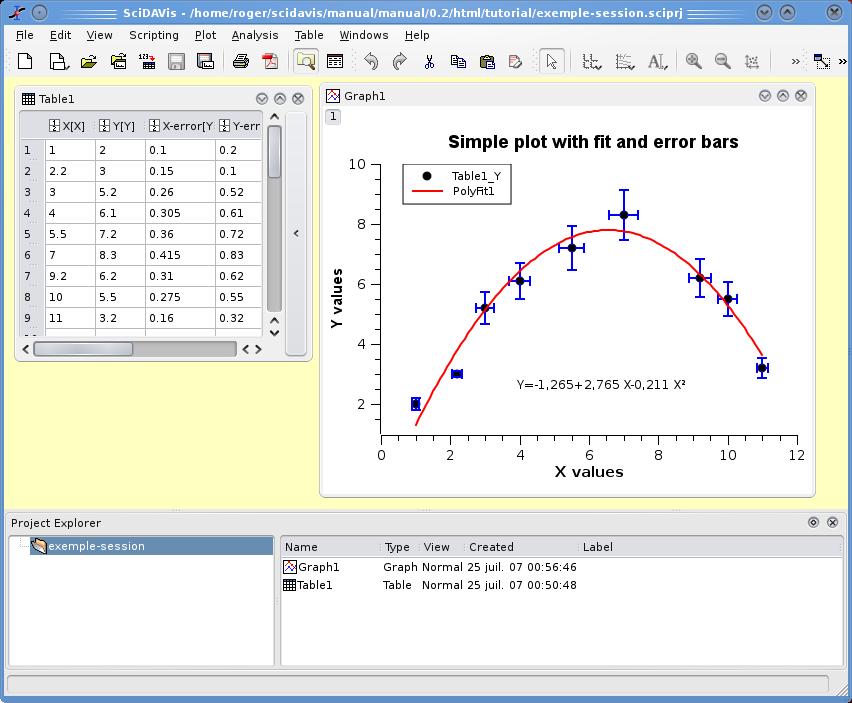
\includegraphics{pics/scidavis-session.png}}
  \caption{A typical \SciDaVis{} session}
  \label{fig-scidavis-session}
\end{figure}

There are numerous commands available in \SciDaVis{} depending on the
element which is selected. Therefore, the main menu bar changes when
you select a particular element of the project. Moreover, you can
access to the set of commands relevant of an element by activating the
context menu with the right button of the mouse.

In a project, the objects which can be used are:

\begin{description}
  \item[Tables]\index{Table}
    A table is a spreadsheet which can be used to store the datas you are entering. It can also be used to do some calculations and statistical analysis of datas. In each table, columns can be labelled as X-values or Y-values for 2D-plotting, or Z-values if you plan to build a 3D-plot. In addition, columns can be labelled as errors on X or on Y values (see \htmlref{Set Column as command}{set-column-as-lnk}).

    A table can be created by the \htmlref{New $\rightarrow$ New Table
      command}{new-table-lnk}. Then there are several ways to fill the
    table with your data. If you want to read a table from an ASCII
    file, you can import the data from the file to a table with the
    \htmlref{Import ASCII command}{import-ascii-lnk}. You can also
    enter each value from the keyboard, or copy and paste from another
    spreadsheet program. The last way to enter your data is to fill
    the table with the results of a mathematical function
    (\htmlref{Assign Formula command}{assign-formula-lnk} from the
    \htmlref{Table menu}{table-menu-lnk})
    
    \item[Matrix]\index{Matrix} A matrix is a
      special table which is used to store the data points for surface
      3D plots. It contains Z-values and doesn't include any column or
      row which could be designated as X-values or
      Y-values. Nevertheless, you can specify the X-values and the
      Y-values with the \htmlref{Set Coordinates
        command}{set-coordinates-lnk} from the \htmlref{Matrix
        menu}{matrix-menu-lnk}.

      A matrix can be created by the \htmlref{New$\rightarrow$ New
        Matrix command}{new-matrix-lnk}. If you want to read a matrix
      from an ASCII file, you can import the data of the file to a
      table with the \htmlref{Import ASCII command}{import-ascii-lnk}
      and then convert this table to a matrix with the \htmlref{Conver
        to Matrix command}{convert-to-matrix-lnk}. In the same way as
      for tables, you can also fill matrix with the results of a
      function $z=f(i,j)$ in which $i$ and $j$ are row and column numbers,
      or $z=f(x,y)$. (see \htmlref{Assign Formula
        command}{assign-formula-lnk} from the \htmlref{Matrix
        menu}{matrix-menu-lnk})

    \item[A Graph]\index{Plot} A graph
      can contain one or several plots. Each of these plots is
      contained in a different {\em layer}, these layers can be
      arranged in many ways to build matrix of plots.

      A new layer can be added to an existing graph with the
      \htmlref{Add Layer command}{add-layer-lnk} from the
      \htmlref{Graph menu}{graph-menu-lnk}. you can also remove an
      existing layer with the \htmlref{Remove Layer
        command}{remove-layer-lnk}, but if you remove a layer, the
      plot will be deleted. You can also copy a layer from one graph
      to another, or copy an existing graph into another, the window
      will be added as a new layer (see the section on
      \htmlref{Multilayer Plots}{sec-multilayer-plots} for more
      details).

      Plots can be created in several ways. You can select data in
      tables or matrix and build a plot, or create new plots from
      functions of one or two variables (see sections \htmlref{2D
        plots}{sec-2d-plots} and \htmlref{3D plots}{sec-3d-plots}).

    \item[A Note] This window is a text
      container which can simply be used to insert comments into a
      project. This object is nevertheless far more powerfull than
      that: it can be used as a calculator, for executing single
      commands and for writing scripts (see the \htmlref{Scripting
        section}{scripting} for more details).
      
    \item[The Log Window]
      This window is used to store the results of all the calculations
      which have been done. If this window is not visible, you can
      find it with the \htmlref{Project
        Explorer}{sec-intro-project-explorer} or with the
      \htmlref{Result Log command}{results-log-lnk}.
      
      The text in the log window is also saved in the project file, so
      that when you load a previously saved project, the results-log
      panel is re-filled with the results of the calculations.

    \item[The Project Explorer]
      This window is used to list all the windows contained in a
      project. The Project Explorer is opened by the \htmlref{Project
        Explorer command}{project-explorer-lnk}, and gives a quick
      access to all elements of a project, hidden or visibles. It can
      be used to do some operations on the windows related to these
      items such as hiding a window, renaming windows, etc.
      
      A project file can include several independant projects. In this case,
      the containers of each project are stored in different folders.

\end{description}
%		General description of a table
%		==============================

\subsection{Tables}\label{sec-intro-table}
\index{Table}

The table is the main part of \SciDaVis{} when working with data. For
controlling and converting data the spreadsheet contains a highly
customizable table: all colors and font preferences can be set using
the \htmlref{Preferences command}{preferences-lnk} of the \htmlref{Edit
  menu}{edit-menu-lnk}. You can resize a table
in terms of rows and columns using the \htmlref{Dimensions command}{table-dimensions-lnk} command
of the \htmlref{Table menu}{table-menu-lnk}. On the left side of the table, the button can
be used to develop the properties tags. This allows to customize the
main parameters of the table.

\begin{figure}
  \resizebox{\textwidth}{!}{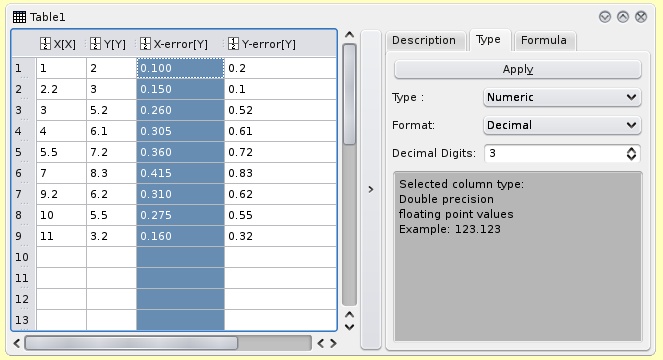
\includegraphics{pics/table.png}}
  \caption{A \SciDaVis{} table with the properties dialog developped
    and the type tag selected.}
  \label{fig-the-table}
\end{figure}

In a spreadsheet, columns can have the following flags: X, Y, Z,
X-error, Y-error or can be simple columns without any special
flag. The X columns are abscissae columns while the Y columns are
ordinates columns used when creating a 2D plot from data. The X-error
and Y-error columns can be used in order to add error bars to 2D
plots. These flags can be changed using the \htmlref{Set Column as
  command}{set-column-as-lnk}.

\index{Table!Number format}

The tag which is selected in figure \ref{fig-the-table} is used to
assign a type to columns: numeric, text, date or time. The format used
to display the data can then be chosen, the format in tables is not
used for plots (use the \htmlref{Axes command}{format-axes-lnk} to
define display format for axes labels).

\begin{figure}
  \resizebox{\textwidth}{!}{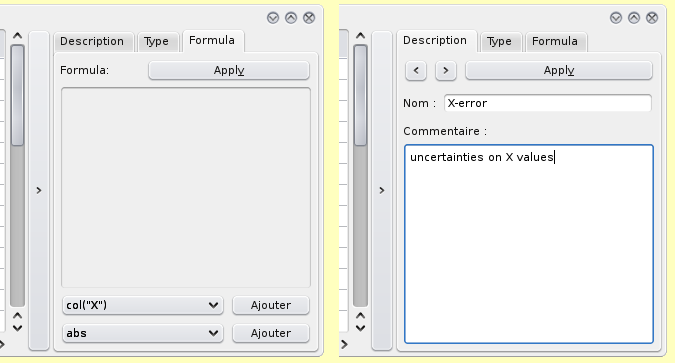
\includegraphics{pics/table_tag_1_3.png}}
  \caption{The two other tags of the properties dialog of \SciDaVis{} tables.}
  \label{fig-the-table_2}
\end{figure}

\index{Table!Labels}

Every column of the table has a label, this can be defined in the
description tag (figure \ref{fig-the-table_2}). This label will be
used by default in plots for curve selection and legend display. You
can use complex labels with spaces and special characters like ``Vol
(cc/g)" if needed. This command can also be reached by the
\htmlref{Edit Column Description command}{edit-column-description-lnk}
of the \htmlref{Table menu}{table-menu-lnk}.

\index{Table!Assign formula}

The last tag of the properties dialog correspond to the command
\htmlref{Assign Formula command}{assign-formula-lnk} of the
\htmlref{Table menu}{table-menu-lnk} (figure \ref{fig-the-table_2}). It is used to fill the column with the result of a mathematic expression. Refer to the \htmlref{Assign Formula command}{assign-formula-lnk} for more details.

You can select all the columns of the spreadsheet (\verb|Ctrl+A|) or
only some of them by clicking on the column label while keeping the
\verb+Ctrl+ key pressed, or by moving the mouse over the column
label. This also allows you to deselect columns.

On the selected columns you can perform various operations:

\begin{itemize}
\item Fill with data. You can insert the row numbers (\htmlref{Fill
  Selection With$\rightarrow$Row Numbers
  command}{fill-selection-with-row-number-lnk}), random numbers
  (\htmlref{Fill Selection With$\rightarrow$Random
  Values}{fill-selection-with-random-values-lnk}), or the result of a
  function (\htmlref{Assign Formula command}{assign-formula-lnk});
\item\index{table!normalize columns} normalize columns with the \verb+Normalize Columns+ command of the context menu;
\item\index{table!sort columns}  sort columns with the \htmlref{Sort
  Table command}{sort-table-lnk} of the \htmlref{Table
  menu}{table-menu-lnk} or with the \verb+sort column+ command of the
  context menu;
\item compute statistical data on columns and rows with the
  \htmlref{Statistics on Columns command}{statistics-on-columns-lnk}
  and \htmlref{Statistics on Rows command}{statistics-on-rows-lnk}
  of the \htmlref{Analysis-tables menu}{analysis-tables-menu-lnk};
\item build a plot from selected columns with the \verb+plot+ command
  of the context menu or with the commands of the \htmlref{Plot menu}{plot-menu-lnk}.
\end{itemize}

All these functions can be reached by right clicking when a column is
selected. Most of them can also be reached by using the \htmlref{Table
  menu}{table-menu-lnk}.

You can cut, copy and paste data between spreadsheets or between a
spreadsheet and another application (Excel, Gnumeric, OpenOffice Calc,
etc).
  
You can import single or multiple ASCII files using the
\htmlref{Import ASCII command}{import-ascii-lnk} from the
\htmlref{File menu}{file-menu-lnk}. This will create one or more new
tables. You can also export the data from the spreadsheet to a text
file using the \htmlref{Export ASCII command}{export-ascii-lnk}.

%		General description of a matrix
%		===============================
\subsection{Matrix}\label{sec-intro-matrix}\index{Matrix}

The matrix is a special table which is used for data which depends on
two variables. This special table is used to store data for
3D-plots. The difference between a table and a matrix is that there is
that columns are assigned to the abscissae x while rows define
abscissae y.

The defaut size of a matrix is $32\times32$ cells. You can modify this size
with the \htmlref{Dimensions command}{matrix-dimensions-lnk}. Column and row numbers are named $i$
and $j$ respectively, ranging from 1 to the size of the matrix. You can
specify an X-scale and an Y-scale with the \htmlref{Set Coordonates command}{set-coordinates-lnk}, this
define values of $x$ and $y$ for columns and rows (figure
\ref{fig-matrix}).

\begin{figure}
  \resizebox{\textwidth}{!}{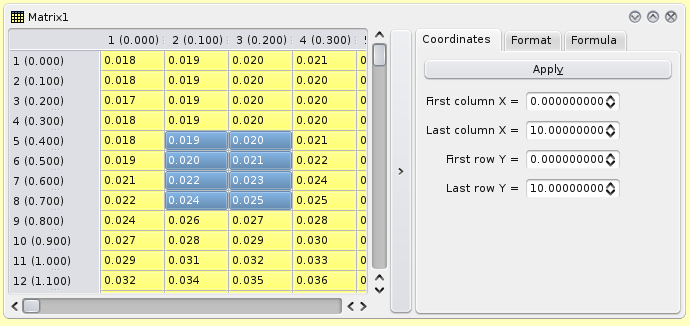
\includegraphics{pics/matrix.png}}
  \caption{The \SciDaVis{} matrix.}
  \label{fig-matrix}
\end{figure}


The values which are stored in a matrix can be obtained from a
function of the form $z=f(i,j)$ or $z=f(x,y)$ with the \htmlref{Assign
  Formula command}{assign-formula-lnk}. They can also be read from a
file with the \htmlref{Import ASCII command}{import-ascii-lnk} which
inserts the file data into a table, and then the table can be
converted to a matrix with the \htmlref{Convert to Matrix
  command}{convert-to-matrix-lnk} of the \htmlref{Matrix
  menu}{matrix-menu-lnk}.

As in the case of tables, a property tag can be shown or hidden by
clicking on the vertical button on the right.

Through the \htmlref{Matrix menu}{matrix-menu-lnk}, several operations can be done on a
matrix like transposition (\htmlref{Transpose command}{transpose-lnk}), mirroring
(\htmlref{Mirror Horizontally command}{mirror-horizontally-lnk} and
\htmlref{Mirror Vertically command}{mirror-vertically-lnk}), inversion
(\htmlref{Invert command}{invert-lnk}), computation of the determinant
(\htmlref{Determinant}{determinant-lnk}). The data of a matrix can then be used to build a
3D plot with the commands present in the \htmlref{plot3d menu}{plot3d-menu-lnk} and in
the \htmlref{3D surface toolbar}{d3-surface-toolbar-lnk}.

%
%</sect2>
%
%<!--
%		General description of a plot window
%		====================================
%-->

\subsection{Plot Window}\label{sec-intro-plot-window}\index{Plot}\index{Plot!Layer}

The plot window is the one in which the graphic is plotted. The main
container of the plot window is the layer. You can have several layers
in a plot, which may be arranged as you want. Each layer can contain a
plot, or another item like a label.

Each new plot can be inserted in a new layer of this plot window, it
has its own geometry and graphic properties (background color, frame,
etc). The figure \ref{fig-plot-window} shows a graph with two layers
which have different geometries. Inside a layer, the area in which the
curves are plotted is the {\em canvas}.

\begin{figure}
  \resizebox{\textwidth}{!}{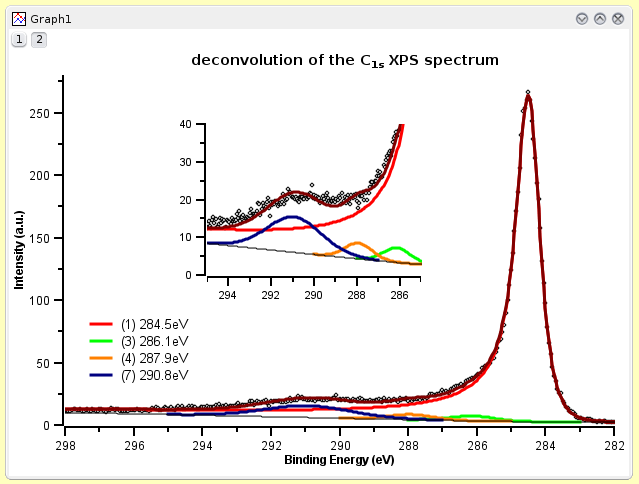
\includegraphics{pics/plot-window.png}}
  \caption{An example of \SciDaVis{} 2D graph with 2 layers.}
  \label{fig-plot-window}
\end{figure}

Each layer can be activated by clicking on the corresponding gray
button  \icon{layer-button.png} in
the top-left corner of the window. The elements which can be accessed
by a double click in a layer are:

%
%<itemizedlist>
%<listitem>
\begin{itemize}
\item the graph itself: this will open the \htmlref{Plot
  details}{format-plot-cmd} dialog box. You can then change the way
  the curves are plotted.
  
\item The axes or the axes labels: this will open the \htmlref{General
  Plot Options Dialog}{format-axes-cmd}. It is used to customize the
  axes, the numbers and labels of the axes, and the grid.
  
\item Any other text item: this will open the \htmlref{Text
  Dialog}{sec-adding-text} which allows to customize the font of the
  label and the frame in which it is drawn.
\end{itemize}

All these functions can be reached through the \htmlref{Format
  menu}{format-menu-lnk}.

%<!--
%		General description of a note
%		=============================
%-->
\subsection{Note}\label{sec-intro-note}
\index{Note}
A note can simply be used to insert text (comments, notes, etc) into a
project, but is really far more powerfull than that. It can be used as
a calculator, for executing single commands and for writing scripts.

\begin{figure}
  \resizebox{\textwidth}{!}{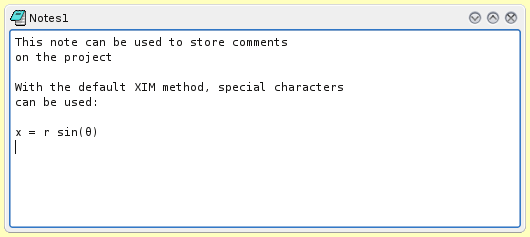
\includegraphics{pics/new-note1.png}}
  \caption{The \SciDaVis{} Note Window.}
  \label{fig-note-window}
\end{figure}

You can also change the text input method. {\em Simple Composing
Input Method} is the standard method to enter text in QT
applications. {\em Xim} is the X input method, it is
the legacy system of the X window environment to support localized
text input. The default choice is the second one, it allows to enter
special characters and accents from your localised environment.

\index{Calculator}
The second use of notes is calculator. The evaluation of mathematical
expressions and execution of code is done via a note's context menu,
the Scripting menu or the convenient keyboard shortcuts. In figure
\ref{fig-note-window-1},
it is shown that you just need to place the cursor on an expression
and use the {\tt Ctrl-Return} command to evaluate the
expression.

\begin{figure}
  \resizebox{\textwidth}{!}{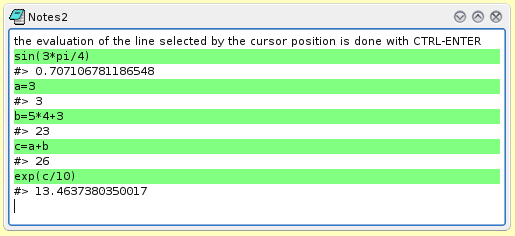
\includegraphics{pics/new-note2.png}}
  \caption{The \SciDaVis{} Note Window used as a calculator.}
  \label{fig-note-window-1}
\end{figure}

you can define variables and refer to them to build complex
expressions, but you must evaluate each line with the
{\tt Ctrl-Return} command to fill the variable with its
value. All variable are private to the note in which it is defined,
and you can't refer to it in another note. With a right click, you
access to the context menu which contains the list of all available
mathematical functions.

For information on expression syntax, supported mathematical functions and how to write scripts, see the \htmlref{scripting section}{scripting}.
%<!--
%		General description of the log window
%		=====================================
%-->
\subsection{Log Window}\label{sec-intro-log-window}

\index{Log Window}
\index{Analysis!Results}

This window keeps a history of all analysis which have been done in
the project. This panel contains the results of all the correlations,
fittings, etc. It can be shown or hidden with the \htmlref{Results Log
  command}{results-log-lnk} of the \htmlref{View menu}{view-menu-lnk}.

\begin{figure}
  \resizebox{\textwidth}{!}{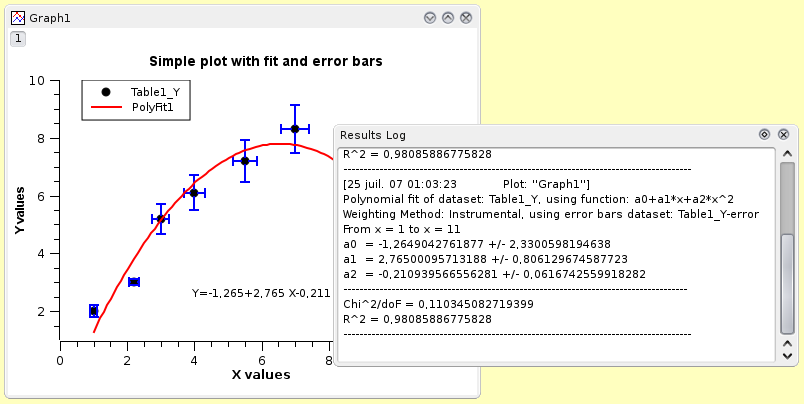
\includegraphics{pics/log-window.png}}
  \caption{The \SciDaVis{} Log window with the information related to a fit on a curve.}
  \label{fig-log-window}
\end{figure}


You can clear the content of the log window with the command
\htmlref{Clear Log Information command}{clear-log-information-lnk} of
the \htmlref{Edit menu}{edit-menu-lnk}. If you load a project for
which some analysis has been done, the computations will be done again
and the log window will be filled with the results.
%<!--
%		General description of the project explorer
%		===========================================
%-->

\subsection{The Project Explorer}\label{sec-intro-project-explorer}
\index{Project Explorer}

The project explorer can be opened/closed using the \htmlref{Project
  Explorer command}{project-explorer-lnk} from the \htmlref{View
  menu}{view-menu-lnk} or by clicking on the \htmlref{Project Explorer
  icon}{project-explorer-icon} in the \htmlref{file toolbar}{sec-file-toolbar}.


\begin{figure}
  \resizebox{\textwidth}{!}{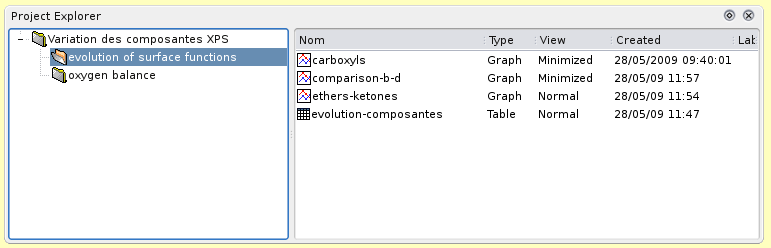
\includegraphics{pics/explorer1.png}}
  \caption{The \SciDaVis{} Project Explorer.}
  \label{fig-project-explorer}
\end{figure}


It gives an overview of the structure of a project and allows the user
to perform various operations on the windows (tables and plots) in the
workspace: hiding, minimazing, closing, renaming, printing,
etc\ldots{} These functions can be reached via the context menu, by
right-clicking on an item in the explorer.

By double-clicking on an item, the corresponding window is shown
maximized in the workspace, even if it was hidden before.

You can organize the differents objects in folders. When selecting a
folder, the default policy is that only the objects contained in it
will be showed in the workspace window. You can also display all the
objects in the subfolders if you change this policy with the ``View
Windows'' command to ``Windows in Active Folder and Subfolders''.



%		tutorial
%		========
%
%	This chapter gives an overview of the features 
%	and a howto to obtain most kinds of plots.

\chapter{Drawing plots with \SciDaVis}

%		2D X-Y plots
%		============

\section{2D X-Y plots}\label{sec-2d-plots}

\index{Plot}
A 2D plot is based on curves which are defined by $Y$ values as
functions of $X$ values. There are different ways to obtain a 2D plot
depending on the way the $(X,Y)$ values are defined:


\begin{enumerate}
  \item You can have your (X,Y) values in a
  \htmlref{table}{sec-intro-table}. You need to select at least one
  column as X values and one column as Y values. This is specified
  with the \htmlref{Set Column As command}{set-column-as-lnk}. Then you can
  select the columns and use one command of the \htmlref{Plot
  menu}{plot-menu-lnk} to plot the data.
  \item If you want to plot a function, you don't need a table. You
  can use directly the \htmlref{New Function Plot
  command}{new-function-plot-lnk}. This will open the corresponding
  dialog box and you will be able to define the mathematical
  expression of your function. In this case, plot can be obtained from
  functions in cartesian coordinates $Y(X)$, but also in parametered
  coordinates $(X(t),Y(t))$, or in angular coordinates $r(\theta)$. 
  \item The combined way is to define a
  \htmlref{table}{sec-intro-table}, and then to fill in the table with
  the results of functions. This can be done with the \htmlref{Assign
  Formula command}{assign-formula-lnk}. Then you can select the
  columns and use one command of the \htmlref{Plot
  menu}{plot-menu-lnk} to plot the data.
  \end{enumerate}  

\SciDaVis{} will create a new graph window, and the plot will be
inserted in a new layer.

Once the plot is created, you can customize all the graphic items of the plot with the commands of the \htmlref{Format Menu}{sec-format-menu}. You can add new items (text labels, lines or arrows, new legend, images) on the plot with the commands of the \htmlref{Graph Menu}{sec-graph-menu}.

%============================================================================
%
%		how to obtain a 2D plot from a table
%

\subsection{2D plot from data.}\label{sec-2d-plot-from-data}
\index{Plot!Create from data}
The data must be stored in a \htmlref{table}{sec-intro-table}. There
are several possibilities to insert your $(X,Y)$ values in the table:
you can write them directly from the keyboard, or read them from a
file. Here we will use the first solution, refer to the
\htmlref{Import ASCII command}{import-ascii-lnk} to use the second one.

The first step is to create an empty project with the \htmlref{New
Project command}{new-project-lnk} from the \htmlref{File
menu}{file-menu-lnk}, you can also use the key \htmlref{New Project
key}{new-project-key} or the \icon{new.png} icon from the \htmlref{File
toolbar}{file-toolbar-lnk}. Then create a new table with the
\htmlref{New Table command}{new-table-lnk} from the \htmlref{File
menu}{file-menu-lnk} or with the \htmlref{New Table
key}{new-table-key} or with the \icon{table.png} icon from the \htmlref{File toolbar}{file-toolbar-lnk}.

At its creation, the table has two column (one for $X$ and one for
$Y$) and 32 rows. You can add rows and columns by selecting a row or a
column and using the right button of the mouse, you can also modify
the number of rows and columns with the \htmlref{Table Dimensions
command}{table-dimensions-lnk} from the \htmlref{Table menu}{table-menu-lnk}. Then, enter your values, and you obtain the table shown in figure \ref{fig-simple-2dplot-1}.

\begin{figure}
  \resizebox{\textwidth}{!}{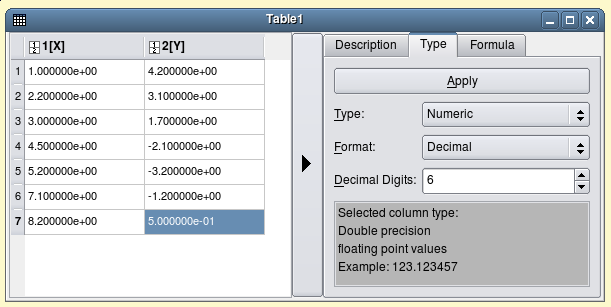
\includegraphics{tutorial/simple-2dplot-1.png}}
  \caption{A simple 2D plot: the table.}
  \label{fig-simple-2dplot-1}
\end{figure}

Then, you have to select the two columns, and build your plot (here a
simple 2D scatter) with the \htmlref{Scatter command}{scatter-lnk}
from the context menu, or by clicking on the corresponding
\icon{pPlot.png} icon from the \htmlref{Plot
toolbar}{plot-toolbar-lnk} or with the \htmlref{Scatter
command}{scatter-lnk} from the \htmlref{Plot menu}{plot-menu-lnk}. A
plot is created which uses the default options for all elements. You
can customize these default options with the \htmlref{2D plot
preferences dialog}{sec-preferences-2d-plot}. With the default
options, you obtain the plot shown in figure
\ref{fig-simple-2dplot-2}.

\begin{figure}
  \resizebox{\textwidth}{!}{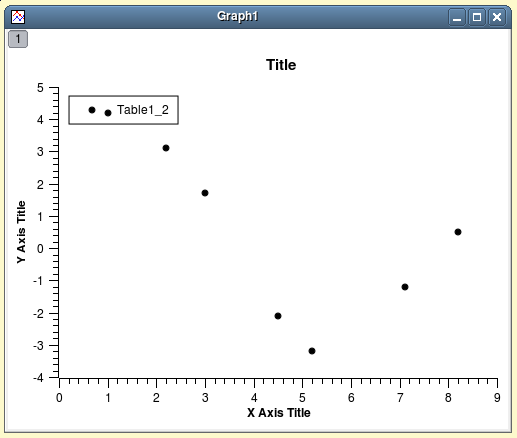
\includegraphics{tutorial/simple-2dplot-2.png}}
  \caption{A simple 2D plot: the default plot.}
  \label{fig-simple-2dplot-2}
\end{figure}

You can now customize your plot with the commands of the
\htmlref{Format menu}{format-menu-lnk}. By double clicking on the data
points, you open the \htmlref{Format plot}{format-plot-lnk} dialog
which is used to modify the symbols. Then a double-click on the axes
opens the \htmlref{Format Axes}{format-axes-lnk} dialog, and you can
change the scales, the fonts for the axes labels, etc. You can also
add grid lines on $X$ or $Y$ axes (\htmlref{Format Grid}{format-grid-lnk}), etc. Finally, a double click on each text item ($X$ title, $Y$ title, plot title) allows to change the text and the presentation of these elements. See the \htmlref{customize section}{sec-customize-2d-plot} for more details. An example of the final plot is shown in figure \ref{fig-simple-2dplot-3}.
%
%<figure id="fig-simple-2dplot-3">
%  <title>A simple 2D plot: the plot finished.</title>
%  <mediaobject> 
%    <imageobject>
%      <imagedata  format="PNG" fileref="tutorial/simple-2dplot-3.png"/>
%    </imageobject>
%  </mediaobject>
%</figure>
\begin{figure}
  \resizebox{\textwidth}{!}{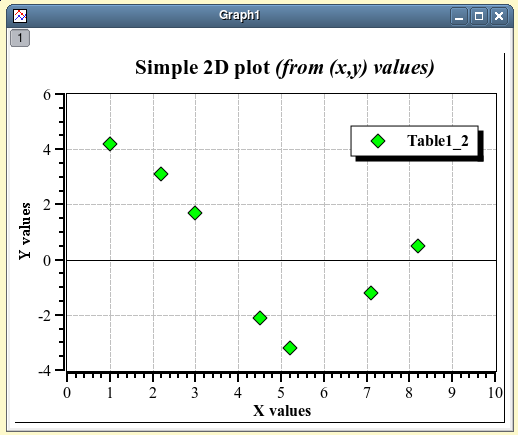
\includegraphics{tutorial/simple-2dplot-3.png}}
  \caption{A simple 2D plot: the plot finished.}
  \label{fig-simple-2dplot-3}
\end{figure}

Finally, you have to save your project in a '.sciprj' file with the
\htmlref{Save Project}{save-project-lnk} from the \htmlref{File
  menu}{file-menu-lnk} or with \html{CTRL+S}{save-project-key} or with
the \icon{filesave.png} icon from the \htmlref{File
  toolbar}. Depending on your application, you can export your plot to
a standard image file with the command  \htmlref{Export
  Graph$\rightarrow$Current command}{export-graph-current-lnk} from
the \htmlref{File menu}{file-menu-lnk} (or with the \htmlref{CTRL+G}{export-graph-current-key} keycode).

\index{Plot!secondary axis}

There are several types of plots which can be built from a table. They
are presented in the \htmlref{Plot menu}{plot-menu-lnk}. One important
feature is that it is possible to use up to four axis for the
data. For example, create a new table, modify its dimension to 4
columns and 7 rows. Then select the third column and set it as $X$
with the \htmlref{Set Column as command}{set-column-as-lnk} from the
\htmlref{Table menu}{table-menu-lnk}; you can then enter the values of two series $(X1,Y1)$ and $(X2,Y2)$ as shown in the figure \ref{fig-two-axes-plot}.
%
%<figure id="fig-two-axes-plot">
%  <title>A table with two series of values (X1,Y1) and (X2,Y2).</title>
%  <mediaobject> 
%    <imageobject>
%      <imagedata  format="PNG" fileref="tutorial/2axes-2dplot-1.png"/>
%    </imageobject>
%  </mediaobject>
%</figure>
\begin{figure}
  \resizebox{\textwidth}{!}{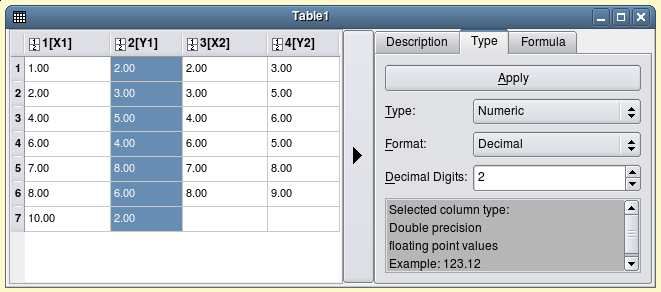
\includegraphics{tutorial/2axes-2dplot-1.png}}
  \caption{A table with two series of values $(X1,Y1)$ and $(X2,Y2)$.}
  \label{fig-two-axes-plot}
\end{figure}

To build the plot, select the two $Y$ columns (select $Y1$, and then
select $Y2$ with CTRL key), use the \htmlref{Plot
  menu}{plot-menu-lnk}. You obtain a simple plot with two axes, then
use the \htmlref{Format Plot}{format-plot-lnk}. In the left window,
select the data serie for which you want to change the axes, click on
the {\em axis} tag and define the axes you want to use. After this,
the plot is modified but the new axes are not shown. Use the
\htmlref{Format Axes command}{format-axes-lnk}, select the new axes
and click on the {\em show} checkbox. You can then customize your plot in order to obtain the result presented in figure \ref{fig-two-axes-plot-1}.


%
%<figure id="fig-two-axes-plot-1">
%  <title>A 2D plot with two Y and two X axis.</title>
%  <mediaobject> 
%    <imageobject>
%      <imagedata  format="PNG" fileref="tutorial/2axes-2dplot-2.png"/>
%    </imageobject>
%  </mediaobject>
%</figure>
\begin{figure}
  \resizebox{\textwidth}{!}{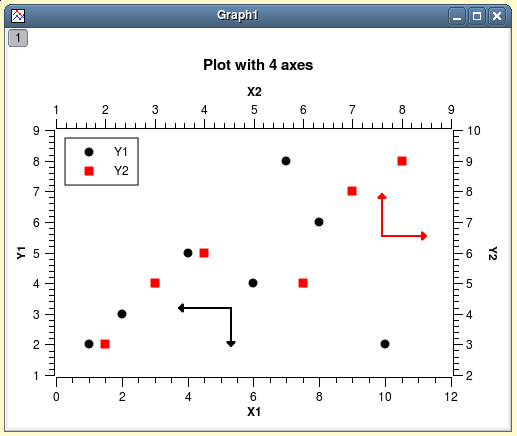
\includegraphics{tutorial/2axes-2dplot-2.png}}
  \caption{A 2D plot with two Y and two X axis.}
  \label{fig-two-axes-plot-1}
\end{figure}

In addition to the customization which has been already described,
four arrows were added with the \htmlref{Draw arrow}{draw-arrow-lnk}.


%		how to obtain a 2D plot from a function
\subsection{2D plot from function.}
\label{sec-2d-plot-from-function}
\index{Plot!Create from function}

There are two ways to obtain such a plot: you can plot directly a
function or fill a table with the values calculated from this function
before doing a plot in the classical way.

\subsubsection{Direct plot of a function.}

If you just want to plot a function, you can use the
\htmlref{New Function Plot}{new-function-plot-lnk} from the
\htmlref{File Menu}{file-menu-lnk} or with the
\htmlref{New Function Plot Key}{new-function-plot-key} or with the
\htmlref{New Function Plot}{new-function-plot-icon} icon from
the \htmlref{File toolbar}{file-toolbar-lnk}.

You can then enter the expression of your mathematical function, the $X$
range used for the plot, and the number of points used in this $X$
range. See the \htmlref{Add Function}{add-function-lnk} for details.

\begin{figure}
  \resizebox{\textwidth}{!}{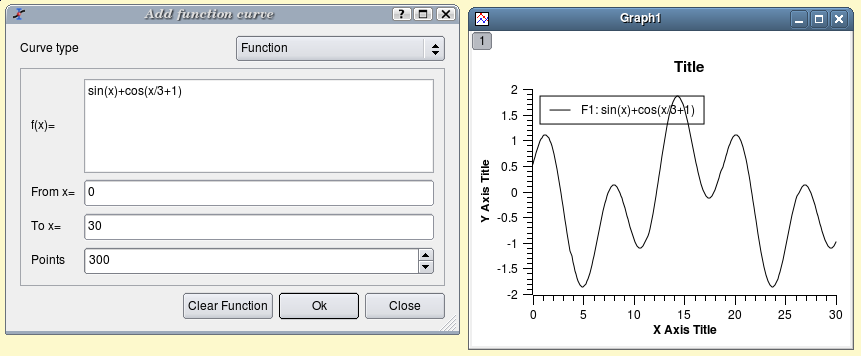
\includegraphics{tutorial/direct-function-plot.png}}
  \caption{Direct plot of a function.}
  \label{fig-direct-function-plot-1}
\end{figure}
%<figure id="fig-direct-function-plot-1">
%  <title>Direct plot of a function.</title>
%  <mediaobject> 
%    <imageobject>
%      <imagedata  format="PNG" fileref="tutorial/direct-function-plot.png"/>
%    </imageobject>
%  </mediaobject>
%</figure>
%


The generic plot which is created by this command can then be
customized as explained in the previous section. Beside classical
$Y=f(X)$ functions, parametric functions and polar functions can be
defined. In parametric coordinates, $X$ and $Y$ are defined as
functions of an independant parameter $m$. You can define these
functions, the range for $m$ and the number of points computed in this
range.

%
%<figure id="fig-direct-function-plot-2">
%  <title>Direct plot of a parametric function.</title>
%  <mediaobject> 
%    <imageobject>
%      <imagedata  format="PNG" fileref="tutorial/direct-function-plot-parametric.png"/>
%    </imageobject>
%  </mediaobject>
%</figure>
%
%<para>Polar coordinate are defined as a radius <emphasis>R</emphasis> and an angle <emphasis>theta</emphasis> (in radian). The coordinates are then obtained by <emphasis>X=R.cos(theta)</emphasis> and <emphasis>Y=R.sin(theta)</emphasis>. You can use a parametric definition: <emphasis>R=f(t)</emphasis> and  <emphasis>theta=f(t)</emphasis>, the range for <emphasis>t</emphasis> and the number of points computed in this range.</para>
%
%<figure id="fig-direct-function-plot-3">
%  <title>Direct plot of a function in polar coordinates.</title>
%  <mediaobject> 
%    <imageobject>
%      <imagedata  format="PNG" fileref="tutorial/direct-function-plot-polar.png"/>
%    </imageobject>
%  </mediaobject>
%</figure>
%
%</sect3>
%<!--
%**********************************************************************
%
%		filling of a table with a function
%
%**********************************************************************
%-->
%<sect3 id="sec-table-function-plot">
%<title>Filling of a table with the values of a function.</title>
%
%<indexterm>
%  <primary>Columns</primary><secondary>Assign formula</secondary>
%</indexterm>
%<para>If you just want to work not only with the plot but also with the data, you can create a new table as explained in the <link linkend="sec-2d-plot-from-data">previous section</link>. Then you can fill this table with the values of a function with the &assign-formula-lnk;. The main advantage of this method is that you can do further analysis of the calculated data as the are kept in a table.</para>
%
%<para>To obtain the same plot as in the previous example, you need to create a new table (key &new-table-key;) and use the &table-dimensions-lnk; to define 300 rows, then select the first column and use the command &assign-formula-lnk; from the context menu, or from the &table-menu-lnk;. The row number symbol is <emphasis>i</emphasis>, so you can enter the function expression <emphasis>i/10</emphasis> (figure <xref xrefstyle="select: labelnumber" linkend="fig-table-function-plot-1"/>).</para>
%
%<figure id="fig-table-function-plot-1">
%  <title>Function plot: filling of the X column.</title>
%  <mediaobject> 
%    <imageobject>
%      <imagedata  format="PNG" fileref="tutorial/table-function-plot1.png"/>
%    </imageobject>
%  </mediaobject>
%</figure>
%
%<para>The second step is to select the second column and use the same command. The expression is a function of the X values, that is the first column named <emphasis>col(1)</emphasis> (figure <xref xrefstyle="select: labelnumber" linkend="fig-table-function-plot-2"/>).</para>
%
%<figure id="fig-table-function-plot-2">
%  <title>Function plot: filling of the Y column.</title>
%  <mediaobject> 
%    <imageobject>
%      <imagedata  format="PNG" fileref="tutorial/table-function-plot2.png"/>
%    </imageobject>
%  </mediaobject>
%</figure>
%
%<para>Once the table is ready, you just have to build the plot as explained in the previous section.</para>
%
%</sect3>
%
%</sect2>
%
%<!--
%*******************************************************************
%
%		Other 2D plots
%		**************
%
%*******************************************************************
%-->
%<sect2 id="sec-other-2d-xy-plot">
%<title>The different types of 2D X-Y plots</title>
%
%<para>Beside the conventional X-Y plots with lines and points, other kinds of plots are available in &appname;. Although the presentation of the data can be very different, they are all based on the use of one column for X values and one column for Y values. Follow the links to the corresponding commands to see a description of these plots.</para>
%
%<para>The first set is available in the subset <emphasis>Special Lines/Symbol</emphasis> of the &plot-menu-lnk;:</para>
%
%<itemizedlist>
%  <listitem>
%    <para>Drop lines plot (&vertical-drop-lines-lnk;)</para>
%  </listitem>
%  <listitem>
%    <para>Scatter plot with a smoothed line connection between the points (&spline-lnk;)</para>
%  </listitem>
%  <listitem>
%    <para>Vertical steps plot (&vertical-steps-lnk;)</para>
%  </listitem>
%  <listitem>
%    <para>Horizontal steps plot (&horizontal-steps-lnk;)</para>
%  </listitem>
%</itemizedlist>
%<para>The other ones are more special plots which can be accessed directly in the &plot-menu-lnk;:</para>
%<itemizedlist>
%  <listitem>
%    <para>Vertical bars plot (&columns-lnk;)</para>
%  </listitem>
%  <listitem>
%    <para>Horizontal bars plot (&rows-lnk;)</para>
%  </listitem>
%  <listitem>
%    <para>Area plot (&area-lnk;)</para>
%  </listitem>
%</itemizedlist>
%
%</sect2>
%
%<!--
%*******************************************************************
%
%		customization of 2D plots
%		*************************
%
%*******************************************************************
%-->
%<sect2 id="sec-customize-2d-plot">
%<title>Customization of a 2D plot</title>
%
%<para>There are many way to improve and modify the plots:</para>
%<itemizedlist>
%  <listitem>
%    <para>The first part of the commands are used to modify the main elements of the plot, that is axis, labels, etc. They can be accessed through the &format-menu-lnk;.</para>
%  </listitem>
%  <listitem>
%    <para>The second part of commands can be used to insert additional objects likes arrows, images, text labels, etc. They can be accessed in the &graph-menu-lnk;.</para>
%  </listitem>
%</itemizedlist>
%<para>This section will show an overview of the first set of commands. See the &graph-menu-lnk; section for the other commands. There are three main windows which allows to modify the plot:</para>
%<itemizedlist>
%  <listitem>
%    <para>The &format-plot-lnk;, it is entitled "Plot details" and is used to customize the global properties of the plot (background color, etc) and the data series (points shape, line width, etc).</para>
%  </listitem>
%  <listitem>
%    <para>The second one is entitled "General plot options" and contain the commands to format axes (scales, labels, grids, etc), it can be accessed through the &format-scales-lnk;, &format-axes-lnk; and &format-grid-lnk;.</para>
%  </listitem>
%  <listitem>
%    <para>The last one is the &format-title-lnk; which is used to control the properties of the title of the plot.</para>
%  </listitem>
%</itemizedlist>
%<para>All these commands are accessed through the &format-menu-lnk;.</para>
%
%<sect3 id="sec-plot-details">
%<title>"Plot details" window</title>
%
%<para>This window has two parts, the left one shows a tree view of the main elements of the plot: the layers and the data series which are plotted in each layer. The main dialog is activated by selecting the &format-plot-lnk; from the &format-menu-lnk;. If it is activated by a double click on a curve in the plot, the same dialog will be opened with the corresponding curve selected (see <link linkend="sec-plot-details-series">next section</link> for details). The right section of the window shows the options which are available for the selected entity. If you do some changes, don't forget to click on the <emphasis>Apply</emphasis> button before switching to another entity.</para>
%
%<sect4 id="sec-plot-details-layer">
%<title>Options for the layer</title>
%
%<indexterm>
%  <primary>Plot details</primary><secondary>Layer options</secondary>
%</indexterm>
%
%<para>This dialog can be used to modify the background color of the global plot area (i.e. the layer), the color of the canvas (that is the area in which curves are plotted), and the border of the plot. This border is for the global plot, if you want to add a border to the canvas, you can use the <emphasis>general</emphasis> tag of the &format-axes-lnk;. If the image format use to save the plots support it, you can also control the transparency of these objects through the opacity parameter. The default value is 255 which means no transparency. See the &export-graph-lnk; for details on image formats.</para> 
%
%<figure id="fig-plot-details-layer">
%  <title>The <emphasis>Plot details</emphasis> Dialog: general properties of the layers.</title>
%  <mediaobject> 
%    <imageobject>
%      <imagedata  format="PNG" fileref="pics/plot-details-layer.png"/>
%    </imageobject>
%  </mediaobject>
%</figure>
%
%</sect4>
%
%<sect4 id="sec-plot-details-series">
%<title>Custom curves for data series</title>
%
%<indexterm>
%  <primary>Plot details</primary><secondary>Options for lines and symbols</secondary>
%</indexterm>
%<para>The commands can be accessed by a double click on a curve, or by using the &format-plot-lnk; and selecting a curve in the window on the left. The right part of the dialog box contains several tabs which depend on the kind of plot that you are using. The left part of the dialog window shows the curves which are plotted in the active layer. All the modifications will be done on the selected curve.</para>
%<!--
%		remark on plot associations buttons
%-->
%<indexterm>
%  <primary>Plot details</primary><secondary>Specification of X and Y series</secondary>
%</indexterm>
%<para>In this dialog box, beside the customization of data curves, you can change the columns which are used by clicking on the <emphasis>Plot Associations...</emphasis> button. This will open a dialog which can be used to select the columns of the table which are used as X and Y values.</para>
%<figure id="fig-plot-associations">
%   <title>The <emphasis>Plot details</emphasis> Dialog: Plot Associations.</title>
%   <mediaobject> 
%      <imageobject>
%         <imagedata  format="PNG" fileref="pics/plot-associations.png"/>
%      </imageobject>
%   </mediaobject>
%</figure>
%
%<para>The button <emphasis>Worksheet</emphasis> can be used to access to the table which contains the columns selected.</para>
%<para>The dialog presented in figure <xref xrefstyle="select: labelnumber" linkend="fig-format-lines"/> is activated for plots drawn with <emphasis>symbols</emphasis>, <emphasis>line+symbols</emphasis>, <emphasis>lines</emphasis>, <emphasis>vertical drop lines</emphasis>, <emphasis>steps</emphasis> and <emphasis>splines</emphasis>. The first tab labelled <emphasis>axis</emphasis> can be used to select the axis which are used for each curve of the plot: bottom (default) or top for abscissae, and left (default) or right for Y values. Beware that whatever your choice the right and top axis will not be drawn, you need to use the &format-axes-lnk; to obtain a plot in which these axis are shown.</para>
%
%<figure id="fig-details-axes">
%  <title>The <emphasis>Plot details</emphasis> Dialog: Choice of axes.</title>
%  <mediaobject> 
%    <imageobject>
%      <imagedata  format="PNG" fileref="pics/plot-details-axes.png"/>
%    </imageobject>
%  </mediaobject>
%</figure>
%
%<para>The second tab allows to modify the style of the line (color, line style, thickness). The connect button allows to change the style which is used to draw the selected curve (steps, droplines, etc). See the &plot-menu-lnk; to see examples of the different types of plot available.</para>
%
%<figure id="fig-format-lines">
%  <title>The Plot details Dialog: Line formatting.</title>
%  <mediaobject> 
%    <imageobject>
%      <imagedata  format="PNG" fileref="pics/plot-details-lines.png"/>
%    </imageobject>
%  </mediaobject>
%</figure>
%
%<para>If you select a style with symbols (scatter or symbol+lines), a last tab can be activated to select the symbol, and to modify the size, the color and the filling color of the symbols.</para>
%
%<figure id="fig-format-symbols">
%  <title>The Plot details Dialog: Symbol formatting.</title>
%  <mediaobject> 
%    <imageobject>
%      <imagedata  format="PNG" fileref="pics/plot-details-symbols.png"/>
%    </imageobject>
%  </mediaobject>
%</figure>
%
%<para>When the data are plotted using bars, the <emphasis>Plot details</emphasis> window shows different options. The first tab named <emphasis>Pattern</emphasis> can be used to customize the background and the border lines of the bars.</para>
%
%<figure id="fig-format-pattern">
%  <title>The Plot details Dialog: Pattern formatting for bars.</title>
%  <mediaobject> 
%    <imageobject>
%      <imagedata  format="PNG" fileref="pics/plot-details-pattern.png"/>
%    </imageobject>
%  </mediaobject>
%</figure>
%
%<para>The second tab named <emphasis>Spacing</emphasis> can be used to modify the geometry of the bars:</para>
%<itemizedlist>
%  <listitem>
%    <para>The default width W of the bar is computed from the smallest difference between two successive abscissae, this correspond to a <emphasis>Gap between bars</emphasis> equal to 0 (which is the default value). All bar are drawn with the same width. The Gap is a percentage of this default width: that is, a value of 50 will decrease the width of all the bars by a factor 2.</para>
%  </listitem>
%  <listitem>
%    <para>The bars are placed in order to be centered around each X value, i.e. between x-W/2 and x+W/2; this correspond to an <emphasis>Offset</emphasis> of 0 (default value). The offset is again a percentage of the default width of the bar. For example, a value of 50 will shift the position of the bar by a half of the default width (W/2) and therefore each bar will placed between x and x+W. Negatives values can be used to shift the bars to the left. If inverted axes are used, the direction of the shift remains the same (i.e. positive offset lead to a shift to the right).</para>
%  </listitem>
%</itemizedlist>
%
%<figure id="fig-format-spacing">
%  <title>The Plot details Dialog: Spacing formatting for bars.</title>
%  <mediaobject> 
%    <imageobject>
%      <imagedata  format="PNG" fileref="pics/plot-details-spacing.png"/>
%    </imageobject>
%  </mediaobject>
%</figure>
%
%</sect4>
%
%</sect3>
%
%</sect2>
%
%<!--
%*******************************************************************
%
%		preferences
%
%*******************************************************************
%-->
%<sect2 id="sec-default-2d-plot">
%
%<title>Changing default 2D plot options</title>
%<indexterm><primary>Options</primary><secondary>2D plot</secondary></indexterm>
%
%<para>There are two ways to modify the default style which is used for plots. The first one applies to all plot and is reached by the &preferences-lnk; (in the &edit-menu-lnk;). And the second one is to define templates for a specific family of plots with the &save-as-template-lnk;.</para>
%
%<sect3 id="sec-preferences-2d-plot">
%<title>Modification of default options</title>
%  <indexterm><primary>Plot</primary><secondary>Change default options</secondary></indexterm>
%  <para>In the dialog box which is opened by the &preferences-cmd;, the third set of options is used to customize the default aspect of <emphasis>2D plots</emphasis>. The first tab is used to set some general options. Most of them are obvious to understand. If <emphasis>autoscaling</emphasis> is set, the scales of the axes will be reset to their default values each time a modification is done on the data series. The <emphasis>scale font</emphasis> option is set by default, in this case the size of the font are modified each time the window size is modified.</para>
%  <figure id="fig-preferences-dialog-3a">
%    <title>The preferences dialog: 2D plot options.</title>
%    <mediaobject>
%      <imageobject>
%        <imagedata  format="PNG" fileref="pics/preferences-dialog3a.png"/>
%      </imageobject>
%    </mediaobject>
%  </figure>
%  <para>The second tab named <emphasis>Curves</emphasis> defines the default style used when you create a new plot.</para>
%  <informalfigure id="fig-preferences-dialog-3b">
%    <mediaobject>
%      <imageobject>
%        <imagedata  format="PNG" fileref="pics/preferences-dialog3b.png"/>
%      </imageobject>
%    </mediaobject>
%  </informalfigure>
%  <para>The third tab named <emphasis>Ticks</emphasis> defines the default style for the ticks of the axes used when you create a new plot.</para>
%  <informalfigure id="fig-preferences-dialog-3c">
%    <mediaobject>
%      <imageobject>
%        <imagedata  format="PNG" fileref="pics/preferences-dialog3c.png"/>
%      </imageobject>
%    </mediaobject>
%  </informalfigure>
%  <para>The fourth tab named <emphasis>Fonts</emphasis> defines the default style for the fonts used for the axes, used when you create a new plot.</para>
%  <informalfigure id="fig-preferences-dialog-3d">
%    <mediaobject>
%      <imageobject>
%        <imagedata  format="PNG" fileref="pics/preferences-dialog3d.png"/>
%      </imageobject>
%    </mediaobject>
%  </informalfigure>
%  <para>The last tab allows to modify two parameters for the printing of plots. The first one is used to re-scale the plot in order to fit the chosen paper size, the other one to print crops marks around the plot (for cutting).</para>
%  <informalfigure id="fig-preferences-dialog-3e">
%    <mediaobject>
%      <imageobject>
%        <imagedata  format="PNG" fileref="pics/preferences-dialog3e.png"/>
%      </imageobject>
%    </mediaobject>
%  </informalfigure>
% </sect3>
%
%</sect2>
%<!--
%=========================================================================
%
%		working with templates
%		======================
%-->
%
%<sect2 id="sec-template-2d-plot">
%  <title>Working with templates</title>
%  <para>If you want to build several plots based on the same model, you can use template files. This allows to save geometry of plots, the values, fonts and colors of labels, etc (see &open-template-lnk; for details on the items which are saved).</para>
%  <para>In the following example, the pristine figure is the <link linkend="fig-simple-2dplot-3">simple 2D plot</link> presented above, it was saved as a template and an empty plot was created by the &open-template-cmd;.</para>
%  <informalfigure id="fig-open-template">
%    <mediaobject> 
%      <imageobject>
%        <imagedata  format="PNG" fileref="pics/template1.png"/>
%      </imageobject>
%    </mediaobject>
%  </informalfigure>
%  <para>You just have to add curves with the &add-remove-curve-lnk;, but the style used to draw the curves is not kept in the template.</para>
%</sect2>
%
%</sect1>
%
%<sect1 id="sec-special-plots">
%<title>Other special 2D plots</title>
%
%<!--
%=========================================================================
%
%		pie plots
%		=========
%-->
%<sect2 id="sec-pie-plots">
%<title>Pie plots</title>
%  <indexterm>
%    <primary>Plot</primary><secondary>pie-plots</secondary>
%  </indexterm>
%
%<para>A pie plot can be built from two columns in a table, the first column will be considered as text and the second as numbers. By default, each sector of the plot will have one label containing the percentages computed from the Y values. Theses labels can be modified as any other  text label.</para>
%
%  <figure id="fig-example-pie">
%    <title>An example of pie plot.</title>
%    <mediaobject>
%      <imageobject>
%        <imagedata  format="PNG" fileref="pics/example-pie.png"/>
%      </imageobject>
%    </mediaobject>
%  </figure>
%
%<sect3 id="sec-format-pie">
%  <title>Formatting of pie plots</title>
%
%  <indexterm>
%    <primary>Plot</primary><secondary>Options for pie-plots</secondary>
%  </indexterm>
%  <para>These commands are available for the plots generated by the &pie-lnk;. The first tab allows the customization of the pie segments. The left fields are used to modify the border which is drawn round each segment: color, type and width of line. The default is no border (line width = 0).</para>
%  <para>The right fields are used to define the filling of the plots. The color button defines the one used for the first segment, then the others segments will have colors which follow the order defined in the list. The default value for this field is black, so segment 2, 3, etc will be red, green, etc.</para>
%  <para>The pattern will be used for all segments of the pie, the default value is solid filling. The last field defines the size of the pie in pixels.</para>
%  <figure id="fig-format-pie">
%    <title>Pie segment formatting.</title>
%    <mediaobject>
%      <imageobject>
%        <imagedata  format="PNG" fileref="pics/format-pie.png"/>
%      </imageobject>
%    </mediaobject>
%  </figure>
%
%</sect3>
%
%</sect2>
%<!--
%=========================================================================
%
%		vectors plots
%		=============
%-->
%<sect2 id="sec-vectors-plots">
%<title>Vectors plots</title>
%  <indexterm>
%    <primary>Plot</primary><secondary>vector-plots</secondary>
%  </indexterm>
%
%  <para>A vector plot can be built from four columns in a table. The two first columns define the position of each arrow in the X-Y drawing area. The two other columns define the length of the arrows, two methods are available for this:</para>
%  <itemizedlist>
%  <listitem>
%    <para><emphasis>Vector-XYXY:</emphasis> the two last columns define the position of the arrow while the two first columns define the origin of the arrow.</para>
%  </listitem>
%  <listitem>
%    <para><emphasis>Vector-XYAM:</emphasis> the two last columns define the angle and the magnitude of the arrow. In this case, the two first columns define the position of the arrow by its origin, its center or its end depending on the options used (see below).</para>
%  </listitem>
%  </itemizedlist>
%
%  <figure id="fig-example-vector">
%    <title>An example of a vector plot (fluid flow around a cylinder in a laminar mode).</title>
%    <mediaobject>
%      <imageobject>
%        <imagedata  format="PNG" fileref="pics/example-vector.png"/>
%      </imageobject>
%    </mediaobject>
%  </figure>
%
%<sect3 id="sec-format-vector">
%  <title>Formatting of vector plots</title>
%
%  <indexterm>
%    <primary>Plot</primary><secondary>Options for vector-plots</secondary>
%  </indexterm>
%
%  <para>In the case of a Vector-XYXY plot, the options window allows to modify the shape and size of the arrow head, and also the linestyle used to draw the arrows.</para>
%
%  <figure id="fig-format-vector-xyxy">
%    <title>Vector-XYXY formatting.</title>
%    <mediaobject>
%      <imageobject>
%        <imagedata  format="PNG" fileref="pics/format-vector-xyxy.png"/>
%      </imageobject>
%    </mediaobject>
%  </figure>
%
%  <para>In the case of a Vector-XYAM plot, the options are the same as above. In addition, the relative position of the arrow as a function of the X-Y values can be specified.</para>
%
%  <figure id="fig-format-vector-xyam">
%    <title>Vector-XYAM formatting.</title>
%    <mediaobject>
%      <imageobject>
%        <imagedata  format="PNG" fileref="pics/format-vector-xyam.png"/>
%      </imageobject>
%    </mediaobject>
%  </figure>
%
%</sect3>
%
%</sect2>
%
%</sect1>
%<!--
%=========================================================================
%
%		statistical plots
%		=================
%-->
%<sect1 id="sec-statistical-plots">
%<title>Statistical plots</title>
%
%<indexterm>
%  <primary>Statistical plots</primary>
%</indexterm>
%
%<para>Statistical plots are different from conventional 2D-plots since they are not use to show the data themselves. Instead, they are able to present the results of some statistical analysis of the data. Following this, histogram are completely different from the plots obtained by the &columns-lnk;.</para>
%
%<sect2 id="sec-box-plots">
%<title>Box plots</title>
%
%<indexterm>
%  <primary>Statistical Plot</primary><secondary>Box plots</secondary>
%</indexterm>
%<sect3 id="sec-box-plots-description">
%<title>Description of box plots</title>
%
%<para>Box plots are used to show some statistical values which are significant parameters of the distribution of the data. Let's assume that we have a table with 12 values in a column. If you select this column and build a box plot with the &box-plot-lnk;, you will obtain a graph which is close to the one presented in the figure <xref xrefstyle="select: labelnumber" linkend="fig-description-box-plot"/>. By default, the values which are computed from your data are (figure <xref xrefstyle="select: labelnumber" linkend="fig-description-box-plot"/>):</para>
%
%<itemizedlist>
%  <listitem>
%    <para><emphasis>Y<subscript>max</subscript></emphasis> The maximum value of Y</para>
%  </listitem>
%  <listitem>
%    <para><emphasis>Y<subscript>5%</subscript></emphasis> The value of Y corresponding to the top 5% of the distribution of numbers</para>
%  </listitem>
%  <listitem>
%    <para><emphasis>Y<subscript>25%</subscript></emphasis> The value of Y corresponding to the top 25% of the distribution of numbers</para>
%  </listitem>
%  <listitem>
%    <para><emphasis>Y<subscript>50%</subscript></emphasis> The value of Y corresponding to the top 50% of the distribution of numbers (also known as the median value)</para>
%  </listitem>
%  <listitem>
%    <para><emphasis>Y<subscript>mean</subscript></emphasis> The average value of Y</para>
%  </listitem>
%  <listitem>
%    <para><emphasis>Y<subscript>75%</subscript></emphasis> The value of Y corresponding to the top 75% of the distribution of numbers</para>
%  </listitem>
%  <listitem>
%    <para><emphasis>Y<subscript>95%</subscript></emphasis> The value of Y corresponding to the top 95% of the distribution of numbers</para>
%  </listitem>
%  <listitem>
%    <para><emphasis>Y<subscript>min</subscript></emphasis> The minimum value of Y</para>
%  </listitem>
%</itemizedlist>
%
%  <figure id="fig-description-box-plot">
%    <title>An example of a box plot for three columns.</title>
%    <mediaobject> 
%      <imageobject>
%        <imagedata  format="PNG" fileref="pics/description-box-plot.png"/>
%      </imageobject>
%    </mediaobject>
%  </figure>
%
%<para>All these parameters give informations on the distribution of data in the column. For example, the difference between <emphasis>Y<subscript>mean</subscript></emphasis> and <emphasis>Y<subscript>50%</subscript></emphasis> is an indication of the symetry of the distribution. Statistical parameters can be used also to compare distribution of data, you just have to select all the columns and build the box plot.</para>
%
%</sect3>
%
%<sect3 id="sec-format-box-plots">
%  <title>Customization of box plots</title>
%
%  <para>There are two ways to modify a box plot: you can modify the statistical parameters which are shown. As in all other plots, you can also modify the appearance of the graphic items.</para>
%
%  <figure id="fig-format-box-1">
%    <title>The Custom Curves Dialog for box: pattern formatting.</title>
%    <mediaobject> 
%      <imageobject>
%        <imagedata  format="PNG" fileref="pics/format-box-1.png"/>
%      </imageobject>
%    </mediaobject>
%  </figure>
%
%  <indexterm>
%    <primary>Whiskers</primary>
%  </indexterm>
%  <para>This tab is used to modify the aspect of the box and of the upper and lower whiskers which are attached to it. You can also remove the box and/or the whiskers.</para>
%  <figure id="fig-format-box-2">
%    <title>The Custom Curves Dialog for box: whiskers formatting.</title>
%    <mediaobject> 
%      <imageobject>
%        <imagedata  format="PNG" fileref="pics/format-box-2.png"/>
%      </imageobject>
%    </mediaobject>
%  </figure>
%
%  <indexterm>
%    <primary>Percentile</primary>
%  </indexterm>
%  <para>As explained above, the default is to draw 3 symbols corresponding to &ymin;, &ymean; and &ymax;. These symbols can be modified (or removed) here. Moreover, you can add two other symbols corresponding to <emphasis>Y<subscript>99%</subscript></emphasis> and <emphasis>Y<subscript>1%</subscript></emphasis>.</para>
%  <figure id="fig-format-box-3">
%    <title>The Custom Curves Dialog for box: percentile formatting.</title>
%    <mediaobject> 
%      <imageobject>
%        <imagedata  format="PNG" fileref="pics/format-box-3.png"/>
%      </imageobject>
%    </mediaobject>
%  </figure>
%
%</sect3>
%
%</sect2>
%
%<sect2 id="sec-histograms">
%  <title>Histograms</title>
%
%  <indexterm>
%    <primary>Statistical Plot</primary><secondary>Histograms</secondary>
%  </indexterm>
%  <indexterm>
%    <primary>Histograms</primary>
%  </indexterm>
%  <sect3 id="sec-description-histograms">
%    <title>Building of an histogram</title>
%
%    <para>An histogram can be used to show the distribution of the values, that is the numbers of values which are in given intervals. Let's assume that you have a set of data in a column. You can select this column and use the &histogram-lnk;. After some customization (see next section), you can obtain a plot like the one presented in the figure <xref xrefstyle="select: labelnumber" linkend="fig-example-histogram"/>.</para>
%
%    <figure id="fig-example-histogram">
%      <title>An example of histogram.</title>
%      <mediaobject> 
%        <imageobject>
%          <imagedata  format="PNG" fileref="pics/example-histogram.png"/>
%        </imageobject>
%      </mediaobject>
%    </figure>
%
%  </sect3>
%
%  <sect3 id="sec-format-histogram">
%    <title>customization of histograms</title>
%
%    <para>As for other plots, you can access to the dialog plot through the &format-plot-lnk; of the &format-menu-lnk;. You can also use the other commands of the &format-menu-lnk; to modify axes, labels, titles, etc. The first tab can used to modify the appearance of the columns: lines and filling.</para>
%    <figure id="fig-format-histogram-1">
%      <title>Pattern formatting in histograms.</title>
%      <mediaobject> 
%        <imageobject>
%          <imagedata  format="PNG" fileref="pics/format-histogram-1.png"/>
%        </imageobject>
%      </mediaobject>
%    </figure>
%    <para>The second tab allows to modify the geometrical parameters of the columns. The parameter <emphasis>gap between bars</emphasis> define the distance between two adjascent columns. This is not a true distance, it define the fraction of space which is occupied by the intervalles between columns. By default, this parameter is at 0% so that there is no space between columns. In the example of figure <xref xrefstyle="select: labelnumber" linkend="fig-example-histogram"/>, a value of 50% has been used, so that the width of space and columns are equal.</para>
%    <para>the second parameter <emphasis>Offset</emphasis> can be used to shift the bars from their default position. For example, In the figure <xref xrefstyle="select: labelnumber" linkend="fig-example-histogram"/>, the number of values between 3 and 4 is 6, and the corresponding column should be plotted at an abscissae of 3.5. In order to have this column corresponding to the value X=3, a negative shift has been applied. The value of the shift is a percentage of the width of the column, the maximum width of the columns is &Delta;X=1 in this example and a a gap of 50% is used so a value of -100% has been used, corresponding to a shift &Delta;X=-0.5.</para>
%    <figure id="fig-format-histogram-2">
%      <title>Whiskers formatting in histograms.</title>
%      <mediaobject> 
%        <imageobject>
%          <imagedata  format="PNG" fileref="pics/format-histogram-2.png"/>
%        </imageobject>
%      </mediaobject>
%    </figure>
%    <para>The last tab is used to define the number of columns used for the plot. It is defined by the X range used for the statistical analysis, and the size of each interval. The default is to use 10 interval in the range [&ymin;:&ymax;].</para>
%    <figure id="fig-format-histogram-3">
%      <title>Interval selection in histograms.</title>
%      <mediaobject> 
%        <imageobject>
%          <imagedata  format="PNG" fileref="pics/format-histogram-3.png"/>
%        </imageobject>
%      </mediaobject>
%    </figure>
%  </sect3>
%
%</sect2>
%
%</sect1>
%
%<!--
%=============================================================================
%
%		3D plots
%		========
%-->
%<sect1 id="sec-3d-plots">
%<title>3D plots</title>
%<indexterm><primary>Surface plot</primary></indexterm>
%<para>3D plot are generated from data defined as <emphasis>Z=f(X,Y)</emphasis>. As for 2D plots, there are two ways to obtain a 3D plot depending on the way the (X,Y,Z) values are defined:</para>
%
%<itemizedlist>
%  <listitem>
%    <para>You can have your Z values in a <link linkend="sec-intro-matrix">matrix</link>. &appname; will consider that all the data present in the matrix are Z values, and the X and Y values can be defined as a linear function of the columns and rows numbers.</para>
%    <para>The data in the matrix can be entered in several ways:</para>
%    <itemizedlist>
%      <listitem>
%        <para>one by one from the keyboard,</para>
%      </listitem>
%      <listitem>
%        <para>by reading an ascii file in a table and converting the table into a matrix,</para>
%      </listitem>
%      <listitem>
%        <para>by setting the values with a function.</para>
%      </listitem>
%    </itemizedlist>
%  </listitem>
%<listitem>
%<para>If you want to plot a function, you don't need a matrix. You can use directly the &new-surface-3d-plot-lnk;.</para>
%</listitem>
%</itemizedlist>
%
%<para>There are several kinds of 3D plots which can be selected, see the &plot3d-menu-lnk; section of the <link linkend="reference">reference chapter</link> for a list of the availables plots.</para>
%
%<figure id="fig-exemple-3dplot">
%  <title>Example of a 3D Plots.</title>
%  <mediaobject> 
%    <imageobject>
%      <imagedata  format="PNG" fileref="pics/exemple-plot3d.png"/>
%    </imageobject>
%  </mediaobject>
%</figure>
%
%<para>
%The 3D plots use OpenGL so you can easily rotate, scale and shift them with the mouse. Via the 3D plot settings dialog or via the Surface 3D Toolbar you can change all the predefined settings of a three dimensional plot: grids, scales, axes, title, legend and colors for the different elements.
%</para>
%
%<para>There are several types of plots which can be built from a matrix. They are presented in the &plot3d-menu-lnk;</para>
%
%<sect2 id="sec-3d-plot-function">
%<title>Direct 3D plot from a function</title>
%
%<indexterm><primary>Surface plot</primary><secondary>Create from function</secondary></indexterm>
%
%<para>This is the simplest way to obtain a 3d plot. It is done with the &new-surface-3d-plot-lnk; from the &file-menu-lnk; or directly with the &new-surface-3d-plot-key;. This will open the following dialog box:</para>
%
%<figure id="fig-define-surface-plot">
%  <title>Definition of a new surface 3D plot</title>
%  <mediaobject> 
%    <imageobject>
%      <imagedata  format="PNG" fileref="pics/define-surface-plot.png"/>
%    </imageobject>
%  </mediaobject>
%</figure>
%
%<para>You can enter the function z=f(x,y) and the ranges for X, Y and Z. Then &appname; will create a default 3d plot:</para>
%
%<figure id="fig-default-surface-plot">
%  <title>The 3D surface plot created by default</title>
%  <mediaobject> 
%    <imageobject>
%      <imagedata  format="PNG" fileref="pics/3D-function-plot-default.png"/>
%    </imageobject>
%  </mediaobject>
%</figure>
%
%<para>You can then customize this plot by opening the <link linkend="sec-customize-3d-plot">Surface plot options dialog</link>. You can modify the axis ranges and parameters, add a title, change the colors of the different items, and modify the aspect ratio of the plot. In addition, you can use the different commands of the &d3-surface-toolbar-lnk; to add grids on the walls or to modify the style of the plot. After some modifications, you can obtain the plot presented above.</para>
%
%<para>If you want to modify the function itself, you can use the <command>surface...</command> command which can be activated from the context menu with a right click on the 3D plot. This will re-open the <emphasis>define surface function dialog box</emphasis>.</para>
%
%<para>The 3D plotting system uses openGL, therefore these plots can be manipulated with the mouse:</para>
%<itemizedlist>
%  <listitem>
%    <para>by clicking on the left button and moving the mouse, you can change the viewpoint of the plot. You can come back to the default viewpoint by clicking on the &reset-rotation-icon; icon of the &d3-surface-toolbar-lnk;.</para>
%  </listitem>
%  <listitem>
%    <para>The ??? can be used to zoom or unzoom the plot. You can come back to the default zoom value by clicking on the &autoscale-icon; icon of the &d3-surface-toolbar-lnk;.</para>
%  </listitem>
%</itemizedlist>
%
%</sect2>
%
%<sect2 id="sec-3d-plot-matrix">
%<title>3D plot from a matrix</title>
%<indexterm><primary>Surface plot</primary><secondary>Create from data</secondary></indexterm>
%<para>The second way to obtain a 3D plot is to use a <link linkend="sec-intro-matrix">matrix</link>. Therefore, the first step is to fill the matrix. This can be done by defining a function.</para>
%<para>The &new-matrix-lnk; create a default empty matrix with 32x32 cells. Then use the &matrix-dimensions-lnk; from the &matrix-menu-lnk; to modify the number of rows and columns of the matrix. The &set-coordinates-lnk; can then be used to define the X and Y ranges. </para>
%<!--
%  <informalfigure>
%    <mediaobject> 
%      <imageobject>
%        <imagedata  format="PNG" fileref="pics/matrix-set-dimensions.png"/>
%      </imageobject>
%    </mediaobject>
%  </informalfigure>
%-->
%<para>Then use the &assign-formula-lnk; to fill the cells with numbers. The ranges of X and Y defined in the previous step are not known by this dialog box, then the function is defined with the row and column numbers (i and j) as entry parameters.</para>
%
%<figure id="fig-assign-formula-matrix">
%  <title>Assigning a multi-lines formula to a matrix</title>
%  <mediaobject> 
%    <imageobject>
%      <imagedata  format="PNG" fileref="pics/assign-formula-matrix.png"/>
%    </imageobject>
%  </mediaobject>
%</figure>
%
%<para>The other way to obtain a matrix is to import an ASCII file into a table with the &import-ascii-lnk; from the &file-menu-lnk;. The table can then be transformed in a matrix with the command &convert-to-matrix-lnk; from the &table-menu-lnk;.</para>
%
%<para>You can then use this matrix to build a 3D plot with one of the command of the &plot-menu-lnk;.</para>
%
%</sect2>
%<!--
%*******************************************************************
%
%		customization of 3D plots
%
%*******************************************************************
%-->
%<sect2 id="sec-customize-3d-plot">
%<title>Customization of a 3D plot</title>
%
%  <indexterm><primary>Surface plot</primary><secondary>Options</secondary></indexterm>
%  <para>A dialog with five tab is activated by double clicking on a contour curve (or on the plotting area) of a 3D plot. It can also be accessed by the commands of the &format-menu-lnk;.</para>
%  <figure id="fig-contour-options-1">
%    <title>The Contour curves options dialog.</title>
%    <mediaobject> 
%      <imageobject>
%        <imagedata  format="PNG" fileref="pics/contour-curve-dialog-1.png"/>
%      </imageobject>
%    </mediaobject>
%  </figure>
%  <para>The first group of settings <emphasis>Scales</emphasis> is used to define the scales of the three axis. It works in the same way as scaling of 2D plots.</para>
%  <informalfigure id="fig-contour-options-2">
%    <mediaobject> 
%      <imageobject>
%        <imagedata  format="PNG" fileref="pics/contour-curve-dialog-2.png"/>
%      </imageobject>
%    </mediaobject>
%  </informalfigure>
%  <para>The second tab <emphasis>Axis</emphasis> is used to define the labels of the three axis. You can also customize the size of the ticks, beware that this size is given in real units. Therefore, it should be chosen in relation to the axis ranges: for example, if you put a length of 1 for the ticks of the X-axis, the length will correspond to a unit of 1 from the Y axis. In the same way, Y and Z ticks are computed in reference to X range.</para>
%  <para>The third tab <emphasis>Title</emphasis> is used to modify the title of the plot. Compared to conventional label dialog box of &appname;, it exhibits some limitations related to the 3D drawing system (no subscripts, superscript, no bold or italic characters). See the &format-title-lnk; for more details.</para>
%     <informalfigure id="fig-contour-options-4">
%    <mediaobject> 
%      <imageobject>
%        <imagedata  format="PNG" fileref="pics/contour-curve-dialog-4.png"/>
%      </imageobject>
%    </mediaobject>
%  </informalfigure>
%  <para>The fourth tab <emphasis>Colors</emphasis> is used to modify the color of the different elements. For <emphasis>General</emphasis> and <emphasis>Coordinate System</emphasis> elements, it is a conventional choosing color dialog box. You can also customize the colormap used to draw the data. See the next section for more details on color maps.</para>
%    <informalfigure id="fig-contour-options-5">
%    <mediaobject> 
%      <imageobject>
%        <imagedata  format="PNG" fileref="pics/contour-curve-dialog-5.png"/>
%      </imageobject>
%    </mediaobject>
%  </informalfigure>
%  <para>The last tab <emphasis>General</emphasis> is used to modify some global parameters of the plots. The <emphasis>orthogonal</emphasis> check box allows to change the 3D view from conventional perspective to orthogonal view. It correspond to the &perspective-icon; icon of the &d3-surface-toolbar-lnk;. The parameter <emphasis>resolution</emphasis> is 1 by default, it indicates that all data points are used to draw the contour curves. If the line network is too dense, you can increase this parameter: with a value of 2 only 1 value over 2 will be used.</para>
%  <para>By default, the plot use the same graphic scales for the three axes. If the ranges are very different, you can adjust the size of the plot by changing the zoom over the different axes. In the example presented above, X and Y ranges are 10 while Z range is 0.2, then a zoom of 3000% should be used for Z axis if the zooms on X and Y are kept at 100%. You can also use the &autoscale-icon; icon of the &d3-surface-toolbar-lnk; to adjust automatically these zoom values.</para>
%
%
%<!--
%*******************************************************************
%
%		Modification of color maps
%
%*******************************************************************
%-->
%<sect3 id="sec-color-schemes">
%<title>Modification of color schemes</title>
%
%  <para>The two colors (data min and data max) defines the color scheme which is used to show the Z-values. They are the colors used for the minimum value of Z (Z<subscript>min</subscript>) and the maximum value of Z (Z<subscript>max</subscript>). We can define the colors by their Red, Green and Blue parameters: [R,G,B]. Then, a value Z will be represented by a color defined as a linear interpolation:</para>
%  <informalequation> 
%  <mediaobject>
%    <imageobject>
%      <imagedata  format="PNG" fileref="equations/equation_couleur.png"/>
%    </imageobject>
%  </mediaobject>
%  </informalequation>
%  <para>The default colors for Z<subscript>min</subscript> and Z<subscript>max</subscript> are respectively blue ( [R,G,B] = [0,0,255] ) and red ( [R,G,B] = [255,0,0] ). This lead to the following color scheme:</para>
%
%  <informalfigure id="fig-default-color-scheme">
%    <mediaobject> 
%      <imageobject>
%        <imagedata  format="PNG" fileref="pics/color-scheme-default.png"/>
%      </imageobject>
%    </mediaobject>
%  </informalfigure>
%
%<para>Another classical color scheme can be built with Z<subscript>min</subscript> = [160,32,32] and Z<subscript>max</subscript> = [255,255,0] (yellow). It leads to:</para>
%
%  <informalfigure id="fig-color-scheme-1">
%    <mediaobject> 
%      <imageobject>
%        <imagedata  format="PNG" fileref="pics/color-scheme-1.png"/>
%      </imageobject>
%    </mediaobject>
%  </informalfigure>
%
%<para>Another way to define colors is to read a colormap from a file. The format of the file is simple: each line defines a color by red, green and blue values as integers between 0 and 255. The numbers should be separated by spaces. You can find several examples of colormaps on the <ulink url="http://sourceforge.net/project/showfiles.php?group_id=78209">QwtPlot3D web site</ulink>.</para>
%</sect3>
%
%</sect2>
%
%<!--
%*******************************************************************
%
%		preferences and use of template
%
%*******************************************************************
%-->
%<sect2 id="sec-default-3d-plot">
%<title>Changing default 3D plot options</title>
%  <indexterm><primary>Surface plot</primary><secondary>Default options</secondary></indexterm>
%  <para>Most of the parameters presented in the previous section can be set by default with the &preferences-lnk; of the &edit-menu-lnk;.</para> 
%  <figure id="fig-preferences-dialog-4">
%    <title>The preferences dialog: 3D plot options.</title>
%    <mediaobject>
%      <imageobject>
%        <imagedata  format="PNG" fileref="pics/preferences-dialog4.png"/>
%      </imageobject>
%    </mediaobject>
%  </figure>
%</sect2>
%
%</sect1>
%<!--
%*******************************************************************
%
%		Multilayer plots
%		****************
%		
%*******************************************************************
%-->
%<sect1 id="sec-multilayer-plots">
%<title>Multilayer Plots</title>
%<indexterm><primary>Multilayers plot</primary></indexterm>
%
%<para>The multilayer windows can contain multiple plots (layers) with different characteristics. Each layer has a corresponding button, which displays a number and is pressed when the layer is the currently active layer. There is only one active layer at a time, and the plot tools (zoom, cursors, drawing tools, delete and move points) can only operate on this layer. Each plot can be made active by clicking on it or on its corresponding button.</para>
%<para>To arrange the layers use the &arrange-layers-lnk;. You can add or remove layers with the &add-layer-lnk; and &remove-layer-lnk; or copy/paste layers from one multilayer window to another. All these functions can be reached via the &graph-menu-lnk;, by using the &plot-toolbar-lnk; or via the context menu (right click in the multilayer window anywhere outside a plot area).</para>
%<para>You can resize and move a layer using the Layer geometry dialog. You can also arrange and resize the plots by hand. A whole plot can be moved by drag and drop: click on the plot and keep the left mouse button pressed.</para>
%<para>By keeping the Shift key pressed and dragging the border of a plot you can scale a plot as needed. When moving the mouse over the borders of a plot, you will see the corresponding arrows.</para>
%<para>You can also use the mouse wheel in order to resize the layers: keeping the Ctrl key pressed and scrolling will resize the hight of the plot canvas, while keeping the Alt key pressed and scrolling will resize its width. By keeping the Shift key pressed and scrolling you can resize the plot in both dimensions.</para>
%
%<sect2 id="sec-building-multilayer-plots-1">
%<title>Building a multilayer plot panel</title>
%
%<para>This is the simplest way to obtain a multilayer plot. It can be used if you want to build a panel of plots with a simple arrangement: 2 plot in a row or in a column, or 4 plots in 2 rows and 2 columns.</para>
%<para>You can select two columns with Y-values in a table, and then use one of the &panel-cmd; commands in the &plot-menu-lnk;. &appname; will create a panel of plots in which the size of the different elements of each plot are synchronized.</para>
%
%  <informalfigure>
%    <mediaobject> 
%      <imageobject>
%        <imagedata format="PNG" fileref="pics/multilayer-panel.png"/>
%      </imageobject>
%    </mediaobject>
%  </informalfigure>
%
%<para>You can then customize the two plots, if you want to change the arrangement of the panel, you can use the &arrange-layers-lnk; from the &graph-menu-lnk;. It must be reminded in this case that each plot is in a layer with a surface which is the half or the quarter of the window surface area. So, if you want to share an element between the two plots (for example a text label), you need to add it in a new layer (see the &add-text-lnk; for more detaile).</para>
%
%</sect2>
%
%<sect2 id="sec-building-multilayer-plots-2">
%<title>Building a multilayer plot step by step</title>
%
%<para>If you need to build a more complex multilayer plot, you can define it step by step.</para>
%<para>The first step is to build your first plot, for example from two columns of a table. We obtain a standard plot window:</para>
%
%  <informalfigure>
%    <mediaobject> 
%      <imageobject>
%        <imagedata  format="PNG" fileref="pics/multilayer-step-1.png"/>
%      </imageobject>
%    </mediaobject>
%  </informalfigure>
%
%<para>Then, select the plot window and use the &add-layer-lnk; from the &graph-menu-lnk;. This will activate a dialog box. If you choose "Guess" you will obtain a panel with two columns, if you choose "corner" you will obtain two superposed layers. If you want to build a panel with two rows or some other regular matrix of plots, you can use the &arrange-layers-lnk; to convert the plot to a panel.</para>
%
%  <informalfigure>
%    <mediaobject> 
%      <imageobject>
%        <imagedata  format="PNG" fileref="pics/multilayer-step-2.png"/>
%      </imageobject>
%    </mediaobject>
%  </informalfigure>
%
%<para>If you want to build a more complex geometry like plots inserted in another one, you can modify the geometry of each plot with the <emphasis>layer geometry</emphasis> command. This command is accessible with the context menu of the layer and it allows to modify the size and the position of each layer. Beware that by default, the background of the different layers are not transparent. Therefore, you must modify this parameter if you want to have some superposition of plots. This modification can be done with the &format-plot-lnk; of the &format-menu-lnk;.</para>
%
%  <informalfigure>
%    <mediaobject> 
%      <imageobject>
%        <imagedata  format="PNG" fileref="pics/multilayer-step-3.png"/>
%      </imageobject>
%    </mediaobject>
%  </informalfigure>
%
%<para>For each layer, you can use the &add-remove-curve-lnk; to select the X and Y values from one of the tables of the project.</para>
%
%  <informalfigure>
%    <mediaobject> 
%      <imageobject>
%        <imagedata  format="PNG" fileref="pics/multilayer-step-4.png"/>
%      </imageobject>
%    </mediaobject>
%  </informalfigure>
%
%<para>After this, you can customize your plot. At the end, the modifications done on the axis or on the axis labels may have modified the geometry of the two plots. You can synchronize again the two plots by applying again the &arrange-layers-lnk;.</para>
%
%</sect2>
%
%</sect1>
%
%
%<sect1 id="sec-adding-objects">
%<title>Adding objects to a plot</title>
%
%<!-- 
%*********************************************************************
%
%		Text options
%
%-->
%<sect2 id="sec-adding-text">
%  <title>Adding a text label</title>
%  <indexterm><primary>Text label</primary><secondary>Properties</secondary></indexterm>
%  <para>This dialog can be opened by several commands such as &format-title-lnk; or when you double click on a text object in your plot. It allows to add/customize the text objects.</para>
%  <figure id="fig-text-options">
%    <title>The text options dialog.</title>
%    <mediaobject> 
%      <imageobject>
%        <imagedata  format="PNG" fileref="pics/text-options-dialog.png"/>
%      </imageobject>
%    </mediaobject>
%  </figure>
%  <para>The <emphasis>Color</emphasis>, <emphasis>Font</emphasis> and <emphasis>Alignment</emphasis> commands allow the modification of the general settings of the text label.</para>
%  <para>The text item can be modified in the text window. Several improvements can be added to the text:</para>
%  <itemizedlist>
%    <listitem><para>&lt;sub&gt;text&lt;/sub&gt; will draw the text as subscripts. You can insert this sequence by clicking on the <inlinemediaobject><imageobject><imagedata  format="PNG" fileref="pics/text-options-icon1.png"/></imageobject></inlinemediaobject>.</para></listitem>
%    <listitem><para>&lt;sup&gt;text&lt;/sup&gt; will draw the text as superscripts. You can insert this sequence by clicking on the <inlinemediaobject><imageobject><imagedata  format="PNG" fileref="pics/text-options-icon2.png"/></imageobject></inlinemediaobject>.</para></listitem>
%    <listitem><para>By clicking on the <inlinemediaobject><imageobject><imagedata  format="PNG" fileref="pics/text-options-icon3.png"/></imageobject></inlinemediaobject>, you can open a new dialog which allows to select greek characters:</para>
%    <informalfigure id="fig-text-options1">
%      <mediaobject> 
%        <imageobject>
%          <imagedata  format="PNG" fileref="pics/text-options-dialog.png"/>
%        </imageobject>
%      </mediaobject>
%    </informalfigure>
%    </listitem>
%    <listitem><para>By clicking on the <inlinemediaobject><imageobject><imagedata  format="PNG" fileref="pics/text-options-icon4.png"/></imageobject></inlinemediaobject>, you can open a new dialog which allows to select various mathematical symbols:</para>
%    <informalfigure id="fig-text-options2">
%      <mediaobject> 
%        <imageobject>
%          <imagedata  format="PNG" fileref="pics/text-options-symbols.png"/>
%        </imageobject>
%      </mediaobject>
%    </informalfigure>
%    </listitem>
%    <listitem><para>&lt;b&gt;text&lt;/b&gt; will draw the text with bold characters. You can insert this sequence by clicking on the <inlinemediaobject><imageobject><imagedata  format="PNG" fileref="pics/text-options-icon5.png"/></imageobject></inlinemediaobject>.</para></listitem>
%    <listitem><para>&lt;i&gt;text&lt;/i&gt; will draw the text with italic characters. You can insert this sequence by clicking on the <inlinemediaobject><imageobject><imagedata  format="PNG" fileref="pics/text-options-icon6.png"/></imageobject></inlinemediaobject>.</para></listitem>
%    <listitem><para>&lt;u&gt;text&lt;/u&gt; will draw the text with underlined characters. You can insert this sequence by clicking on the <inlinemediaobject><imageobject><imagedata  format="PNG" fileref="pics/text-options-icon7.png"/></imageobject></inlinemediaobject>.</para></listitem>
%  </itemizedlist>
%</sect2>
%
%</sect1>
%

<!--

		SMALL TUTORIAL ON THE ANALYSIS POSSIBILITIES
		============================================

		rewrited and updated for version 0.20

-->
<title>Analysis of data and curves</title>

<!--
*************************************************************************

				FFT

*************************************************************************
-->
<sect1 id="sec-fft">
<title>Fast Fourier Transform</title>

<indexterm><primary>Curve analysis</primary><secondary>FFT</secondary></indexterm>

<para>This function can be accessed by the &fft-on-curves-lnk; of the &analysis-tables-menu-lnk; when a table is selected, or &analysis-plots-menu-lnk; when a plot is selected. The Fourier transform decomposes a signal in its elementary components by assuming that the signal x(t) can be describe as a sum:</para>

<equation> 
  <title>Fourier equation</title>
  <mediaobject>
    <imageobject>
      <imagedata format="PNG" fileref="equations/equation_fourier.png"/>
    </imageobject>
  </mediaobject>
</equation>

<para>in which ω<subscript>n</subscript> are the frequencies, a<subscript>n</subscript> are the amplitudes of each frequency and ψ<subscript>n</subscript> are the phase corresponding frequency. &appname; will compute these parameters and build a new plot of the amplitude as a function of the frequency. FFT can be performed on a curve to extract the characteristic frequencies.</para>
<para>Let's assume you have the signal presented in the next figure. You can select the &fft-on-curves-lnk; of the &analysis-plots-menu-lnk; to open the FFT dialog box.</para>

<figure id="fig-exemple-fft-1">
  <title>A signal and the FFT dialog box for a plot.</title>
  <mediaobject> 
    <imageobject>
      <imagedata  format="PNG" fileref="pics/exemple-fft-1.png"/>
    </imageobject>
  </mediaobject>
</figure>

<para>If the <emphasis>Normalize Amplitude</emphasis> check box is on, the amplitude curve is normalized to 1. If the <emphasis>Shift Results</emphasis> check box is on, the frequencies are shifted in order to obtain a centered x-scale. By default, the <emphasis>Sampling Interval</emphasis> corresponds to the interval between X-values. Giving a smaller value makes no sense, but you can increase this value in order to sample less values.</para>
<para>&appname; will create a new plot window with the FFT amplitude curve, and a new table which contains the real part, the imaginary part, the amplitude, and the angle of the FFT. In this example, the amplitude curve has been normalized, and the frequencies have been shifted to obtain a centered x-scale.</para>

<figure id="fig-exemple-fft-2">
  <title>The resulting FFT with the characteristic frequencies.</title>
  <mediaobject> 
    <imageobject>
      <imagedata  format="PNG" fileref="pics/exemple-fft-2.png"/>
    </imageobject>
  </mediaobject>
</figure>


<para>In the case of a table, you must select the sampling column (X-values) and one columns (for real numbers) or two columns (for complex numbers) for Y-values.</para>

<figure id="fig-exemple-fft-3">
  <title>The &fft-on-tables-cmd; dialog box for a table.</title>
  <mediaobject> 
    <imageobject>
      <imagedata  format="PNG" fileref="pics/exemple-fft-3.png"/>
    </imageobject>
  </mediaobject>
</figure>

</sect1>

<!--
*******************************************************************************

			Filtering of data and curves

*******************************************************************************
-->
<sect1 id="sec-filtering">
<title>Filtering of data curves</title>
<indexterm><primary>Filtering</primary><see>Curve analysis</see></indexterm>
<indexterm><primary>Curve analysis</primary><secondary>Curve filtering</secondary></indexterm>

<para>In this section, it will be assumed that you have the signal presented in the previous section (see figure <xref linkend="fig-exemple-fft-1"/>). We can analyze this signal by doing a FFT on the data curve and it will show that this signal has a power spectrum with high and low frequencies (see figure <xref linkend="fig-exemple-fft-2"/>). The newt sections will show the influence of the different filters on this data curve.</para>

<sect2 id="sec-fft-filter-low">
<title>FFT low pass filter</title>
<indexterm><primary>Curve analysis</primary><secondary>Curve filtering</secondary><tertiary>Low pass FFT</tertiary></indexterm>

<para>This filter allows to cut the high frequencies of a signal. You just have to select the cut-off frequency of the filter. Let us assume that we want to keep the frequencies below 1.5 Hz, we will obtain:</para>
  <figure id="fig-filter-fft-low-signal">
  <title>Signal after a FFT low pass filter</title>
    <mediaobject> 
      <imageobject>
        <imagedata  format="PNG" fileref="pics/filter-fft-low-signal.png"/>
      </imageobject>
    </mediaobject>
  </figure>
  <para>The power spectrum of this new signal shows that the frequencies below 1.5 Hz have been kept.</para>
  <informalfigure id="fig-filter-fft-low-power">
    <mediaobject> 
      <imageobject>
        <imagedata  format="PNG" fileref="pics/filter-fft-low-power.png"/>
      </imageobject>
    </mediaobject>
  </informalfigure>
</sect2>

<sect2 id="sec-fft-filter-high">
<title>FFT high pass filter</title>
<indexterm><primary>Curve analysis</primary><secondary>Curve filtering</secondary><tertiary>High pass FFT</tertiary></indexterm>

<para>This filter allows to cut the low frequencies of a signal. You just have to select the cut-off frequency of the filter. Let us assume that we want to keep the frequencies above 1.5 Hz, we will obtain:</para>
  <figure id="fig-filter-fft-high-signal">
  <title>Signal after a FFT high pass filter</title>
    <mediaobject> 
      <imageobject>
        <imagedata  format="PNG" fileref="pics/filter-fft-high-signal.png"/>
      </imageobject>
    </mediaobject>
  </figure>
  <para>The power spectrum of this new signal shows that the frequencies above 1 Hz have been kept.</para>
  <informalfigure id="fig-filter-fft-high-power">
    <mediaobject> 
      <imageobject>
        <imagedata  format="PNG" fileref="pics/filter-fft-high-power.png"/>
      </imageobject>
    </mediaobject>
  </informalfigure>
</sect2>

<sect2 id="sec-fft-filter-band">
<title>FFT band pass filter</title>
<indexterm><primary>Curve analysis</primary><secondary>Curve filtering</secondary><tertiary>Band pass FFT</tertiary></indexterm>

<para>This filter allows to cut the low and high frequencies of a signal. You just have to select the high and low cut-off frequencies of the filter. Let us assume that we want to keep the frequencies between 1.5 and 3.5 Hz, we will obtain:</para>
  <figure id="fig-filter-fft-band-signal">
  <title>Signal after a FFT band pass filter</title>
    <mediaobject> 
      <imageobject>
        <imagedata  format="PNG" fileref="pics/filter-fft-band-signal.png"/>
      </imageobject>
    </mediaobject>
  </figure>
  <para>The power spectrum of this new signal shows that only the frequencies at 1.5 and 3.5 Hz have been kept.</para>
  <informalfigure id="fig-filter-fft-band-power">
    <mediaobject> 
      <imageobject>
        <imagedata  format="PNG" fileref="pics/filter-fft-band-power.png"/>
      </imageobject>
    </mediaobject>
  </informalfigure>
</sect2>

<sect2 id="sec-fft-filter-block">
<title>FFT block band filter</title>
<indexterm><primary>Curve analysis</primary><secondary>Curve filtering</secondary><tertiary>Block pass FFT</tertiary></indexterm>

<para>This filter allows to keep the low and high frequencies of a signal. You just have to select the high and low cut-off frequencies of the filter. Let us assume that we want to remove the frequencies between 1.5 and 3.5 Hz, we will obtain:</para>
  <figure id="fig-filter-fft-block-signal">
  <title>Signal after a FFT block band filter</title>
    <mediaobject> 
      <imageobject>
        <imagedata  format="PNG" fileref="pics/filter-fft-block-signal.png"/>
      </imageobject>
    </mediaobject>
  </figure>
  <para>The power spectrum of this new signal shows that only the frequencies below 1.5 Hz and above 3.5 Hz have been kept.</para>
  <informalfigure id="fig-filter-fft-block-power">
    <mediaobject> 
      <imageobject>
        <imagedata  format="PNG" fileref="pics/filter-fft-block-power.png"/>
      </imageobject>
    </mediaobject>
  </informalfigure>
</sect2>
</sect1>

<!--
*************************************************************************

		Correlation and autocorrelation

*************************************************************************
-->
<sect1 id="sec-correlate">
<title>Correlation and autocorrelation</title>

<indexterm><primary>Table analysis</primary><secondary>Correlation function</secondary></indexterm>

<para>This function can be accessed by the &correlate-lnk; of the &analysis-tables-menu-lnk; when a table is selected. The correlation function, also known as the covariance function is used to test the similarity of two signals <emphasis>x(t)</emphasis> and <emphasis>y(t)</emphasis>. It is computed by:</para>

<equation> 
	<title></title>
  <mediaobject>
    <imageobject>
      <imagedata format="PNG" fileref="equations/equation_covariance.png"/>
    </imageobject>
  </mediaobject>
</equation>

<para>in which <inlineequation><graphic fileref="equations/equation_x-m.png"/></inlineequation> and <inlineequation><graphic fileref="equations/equation_y-m.png"/></inlineequation> are the mean values of the signals <emphasis>x(t)</emphasis> and <emphasis>y(t)</emphasis> respectively. If the number of points is <emphasis>N</emphasis>, the function will be computed between <emphasis>-N/2</emphasis> and <emphasis>N/2</emphasis>. The abscissas are therefore point numbers and not <emphasis>t</emphasis> values.</para>
<para>To perform a cross correlation between two signal, they must be in the same table and use the same abscissa. You just have to select the two columns in the table, and select the  &correlate-lnk; from the &analysis-tables-menu-lnk;. A plot will be created and the values of the correlation function will be added as two new columns in the table.</para>

<figure id="fig-exemple-correlation-1">
  <title>An example of a correlation between two functions: the two signals.</title>
  <mediaobject> 
    <imageobject>
      <imagedata  format="PNG" fileref="pics/exemple-correlation-1.png"/>
    </imageobject>
  </mediaobject>
</figure>

<figure id="fig-exemple-correlation-2">
  <title>An example of a correlation between two functions: the correlation function.</title>
  <mediaobject> 
    <imageobject>
      <imagedata  format="PNG" fileref="pics/exemple-correlation-2.png"/>
    </imageobject>
  </mediaobject>
</figure>

<para>The correlation of a signal with itself can also be used in spectral analysis (it is then called autocorrelation or autocovariance function). This operation can be performed by selecting one column in a table and use the &autocorrelate-lnk; from the &analysis-tables-menu-lnk;.</para>

</sect1>
<!--
*************************************************************************

				Convolution

*************************************************************************
		TODO, I don't understand the results...
-->
<sect1 id="sec-convolute">
<title>Convolution of functions</title>
<indexterm><primary>Table analysis</primary><secondary>Convolution</secondary></indexterm>

<para>This function can be accessed by the &convolute-lnk; of the &analysis-tables-menu-lnk; when a table is selected. The convolution of two functions <emphasis>f<subscript>1</subscript>(x)</emphasis> and <emphasis>f<subscript>2</subscript>(x)</emphasis> is the function defined  by:</para>

<!-- TODO
<equation> 
  <mediaobject>
    <imageobject>
      <imagedata format="PNG" fileref="equations/equation_convolution.png"/>
    </imageobject>
  </mediaobject>
</equation>
-->

<para><emphasis>f<subscript>1</subscript>(x)</emphasis> is the signal and <emphasis>f<subscript>2</subscript>(x)</emphasis> is the transfer function.</para>

</sect1>
<!--
*************************************************************************

				Deconvolution

*************************************************************************
		TODO...
-->
<sect1 id="sec-deconvolute">
<title>Deconvolution</title>
<indexterm><primary>Table analysis</primary><secondary>Deconvolution</secondary></indexterm>

<para>This function can be accessed by the &deconvolute-lnk; of the &analysis-tables-menu-lnk; when a table is selected. The deconvolution is the inverse of convolution, that is finding the function <emphasis>f<subscript>1</subscript>(x)</emphasis> which is the solution of the equation <emphasis>f<subscript>1</subscript>*f<subscript>2</subscript>=g</emphasis>.</para>

</sect1>
<!--
*************************************************************************

			Fitting of data and curves

*************************************************************************
-->
<sect1 id="sec-fitting">
<title>Fitting of data and curves</title>

<para>Fitting can be done in two ways:</para>
<itemizedlist>
  <listitem>
    <para>A general <emphasis>Fit Wizard</emphasis> which allows to use complex functions and to adjust the fitting parameters.</para>
  </listitem>
  <listitem>
    <para>A set of simplified fitting dialog boxes for most used functions like exponential growth or decay, etc.</para>
  </listitem>
</itemizedlist>
<!--
			General non linear fit
-->
<sect2 id="sec-non-linear-curve-fit">
<title>Non Linear Curve Fit</title>

<indexterm><primary>Curve analysis</primary><secondary>Curve fitting</secondary><tertiary>Non linear function</tertiary></indexterm>

<para>This function can be accessed by the &fit-wizard-plot-lnk; of the &analysis-plots-menu-lnk; when a plot is selected, or the &analysis-tables-menu-lnk; when aa table window is selected. In the latter case, this command first creates a new plot window using the list of selected columns in the table.</para>
<para>This Command is used to fit discrete data points with a mathematical function. The fitting is done by minimizing the least square difference between the data points and the Y values of the function.</para>

<sidebar>
  <title>Note:</title>
  <para>If the data points are modified, the fit is not re-calculated. Then, you need to remove the old fitted curve and to redo the fit with the same function and the new points.</para>
</sidebar>

<para>The top of the dialog box is used to choose a function among the one which are already define. Four types of functions are available: the user defined functions which have been saved, the classical functions proposed by &appname; in the analysis menu, the simple elementary built-in functions, and external functions via pluggins.</para>
<para>To choose one of these functions, you just have to select it and to click on the checkbox under the selector.</para>
<para>If you want to define your own function, you can use the bottom half of the dialog box. You can write you own mathematical expression or add expressions obtained with the function selector. Then you need to define the parameters which have to be fitted in a comma separated list.</para>

<figure id="fig-non-linear-curve-fit-1">
  <title>The first step of the &fit-wizard-plot-cmd; dialog box.</title>
  <mediaobject> 
    <imageobject>
      <imagedata  format="PNG" fileref="pics/fit-dialog1.png"/>
    </imageobject>
  </mediaobject>
</figure>

<para>The second step is to define the parameters for the fit. You have to give initial guess for the fitting parameters.</para>

<figure id="fig-non-linear-curve-fit-2">
  <title>The second step of the &fit-wizard-plot-cmd; dialog box.</title>
  <mediaobject> 
    <imageobject>
      <imagedata  format="PNG" fileref="pics/fit-dialog2.png"/>
    </imageobject>
  </mediaobject>
</figure>

<para> In this second tab you can also choose a weighting method for your fit (the default is <emphasis>No weighting</emphasis>). The available weighting methods are:</para>
<orderedlist>
  <listitem>
    <para><emphasis>Instrumental</emphasis>: the values of the associated error bars are used as weighting coefficients. You must add Y-error bars to the analyzed curve before performing the fit.</para>
  </listitem>
  <listitem>
    <para><emphasis>Statistical</emphasis>: the weighting coefficients are calculated as the square-roots of each data point in the fitted curve.</para>
  </listitem>
  <listitem>
    <para><emphasis>Arbitrary Dataset</emphasis>: you have the possibility to set the weighting coefficients using an arbitrary data set. The column used for the weighting must have a number of rows equal to the number of points in the fitted curve. </para>
  </listitem>
</orderedlist>

<para>After the fit, the log window is opened to show the results of the fitting process.</para>
<para>Depending on the settings in the <emphasis>Custom Output</emphasis> tab, a function curve (option <emphasis>Uniform X Function</emphasis>) or a new table (if you choose the option <emphasis>Same X as Fitting Data</emphasis>) will be created for each fit. The new table includes all the X and Y values used to compute and to plot the fitted function and is hidden by default, but it can be found and viewed with the <link linkend="project-explorer-cmd">project explorer</link>.</para>

<figure id="fig-non-linear-curve-fit-3">
  <title>The results of the &fit-wizard-plot-cmd;.</title>
  <informalexample>
    <para>The results are shown in the log window, the curve is plotted in the active window, and a table is created to store the fit.</para>
  </informalexample>
  <mediaobject> 
    <imageobject>
      <imagedata  format="PNG"  fileref="pics/fit-dialog3.png"/>
    </imageobject>
  </mediaobject>
</figure>

</sect2>
<!--
			Fitting to specific functions
-->
<sect2 id="sec-ajustements-specifiques">
<title>Fitting to specific curves</title>

<para>&appname; include quick access to the most usefull functions for fitting. Beware that when you use these commands, &appname; uses default values as initial guesses for the parameters. Therefore, the convergence may be difficult or even impossible if these initial values are too far from the final values. In this case, you can use the &fit-wizard-table-lnk; or the &fit-wizard-plot-lnk;, select the function in the <emphasis>built-in</emphasis> set and give good initial values for parameters.</para>

<sect3 id="sec-fit-linear">

  <title>Fitting to a line</title>
  <indexterm><primary>Curve analysis</primary><secondary>Curve fitting</secondary><tertiary>line</tertiary></indexterm>

  <para>This command is used to fit a curve which has a linear shape. The results will be given in the <link linkend="sec-intro-log-window">Log panel</link>.</para>

  <figure id="fig-fit-linear">
    <title>The results of a &fit-linear-cmd;.</title>
    <mediaobject> 
      <imageobject>
        <imagedata  format="PNG" fileref="pics/fit-linear.png"/>
      </imageobject>
    </mediaobject>
  </figure>

</sect3>

<sect3 id="sec-fit-polynomial">

  <title>Fitting to a polynomial</title>
  <indexterm><primary>Curve analysis</primary><secondary>Curve fitting</secondary><tertiary>Polynomial</tertiary></indexterm>

  <para>This command is used to fit a curve which has a linear shape. The results will be given in the <link linkend="sec-intro-log-window">Log panel</link></para>

  <informalfigure id="fig-fit-polynomial-dialog">
    <mediaobject> 
      <imageobject>
        <imagedata  format="PNG" fileref="pics/fit-polynomial.png"/>
      </imageobject>
    </mediaobject>
  </informalfigure>

</sect3>


<sect3 id="sec-fit-bolzmann">
<title>Fitting to a Bolzmann function</title>
<indexterm><primary>Curve analysis</primary><secondary>Curve fitting</secondary><tertiary>Bolzmann function</tertiary></indexterm>

<para>This command is used to fit a curve which has a sigmoidal shape. The function used is:</para>

<equation> 
  <title>Bolzmann equation</title>
  <mediaobject>
    <imageobject>
      <imagedata  format="PNG" fileref="equations/equation_bolzmann.png"/>
    </imageobject>
  </mediaobject>
</equation>

<para>in which A<subscript>2</subscript> is the high Y limit, A<subscript>1</subscript> is the low Y limit, x<subscript>0</subscript> is the inflexion point and dx is the width.</para>

  <figure id="fig-fit-bolzman">
    <title>The results of a &fit-bolzmann-cmd;.</title>
    <mediaobject> 
      <imageobject>
        <imagedata  format="PNG" fileref="pics/fit-sigmoidal.png"/>
      </imageobject>
    </mediaobject>
  </figure>

</sect3>

<sect3 id="sec-fit-gaussian">
<title>Fitting to a Gauss function</title>
<indexterm><primary>Curve analysis</primary><secondary>Curve fitting</secondary><tertiary>Gaussian function</tertiary></indexterm>

<para>This command is used to fit a curve which has a bell shape. The function used is:</para>

<equation> 
  <title>Gauss equation</title>
  <mediaobject>
    <imageobject>
      <imagedata  format="PNG" fileref="equations/equation_gauss.png"/>
    </imageobject>
  </mediaobject>
</equation>

<para>in which A is the height, w is the width, x<subscript>c</subscript> is the center and y<subscript>0</subscript> is the Y-values offset.</para>

  <figure id="fig-fit-gauss">
    <title>The results of a &fit-gaussian-cmd;.</title>
    <mediaobject> 
      <imageobject>
        <imagedata  format="PNG" fileref="pics/fit-gaussian.png"/>
      </imageobject>
   </mediaobject>
  </figure>

</sect3>

<sect3 id="sec-fit-lorentzian">
<title>Fitting to a Lorentz function</title>
<indexterm><primary>Curve analysis</primary><secondary>Curve fitting</secondary><tertiary>Lorentz function</tertiary></indexterm>

<para>This command is used to fit a curve which has a bell shape. The function used is:</para>

<equation> 
  <title>Lorentz equation</title>
  <mediaobject>
    <imageobject>
      <imagedata  format="PNG" fileref="equations/equation_lorentz.png"/>
    </imageobject>
  </mediaobject>
</equation>

<para>in which A is the area, w is the width, x<subscript>c</subscript> is the center and y<subscript>0</subscript> is the Y-values offset.</para>

  <figure id="fig-fit-lorentz">
    <title>The results of a &fit-lorentzian-cmd;.</title>
    <mediaobject> 
      <imageobject>
        <imagedata  format="PNG" fileref="pics/fit-lorentzian.png"/>
      </imageobject>
    </mediaobject>
  </figure>

</sect3>

</sect2>

<sect2 id="sec-fit-multipeak">
<title>Multi-Peaks fitting</title>
<indexterm><primary>Curve analysis</primary><secondary>Curve fitting</secondary><tertiary>Multi peak</tertiary></indexterm>

<para>This kind of fitting allows to fit your data points to a sum of N Gaussian or Lorentzian functions. The first step is to specify the number of peaks. Then you must define the position of each peak on the curve. This is done by selecting one data point on the plot, then validate your choice for each peak with the <emphasis>ENTER</emphasis> key.</para>
  <figure id="fig-fit-multipeak">
    <title>The selection of the position of the peaks.</title>
    <mediaobject> 
      <imageobject>
        <imagedata  format="PNG" fileref="pics/fit-multipeak-1.png"/>
      </imageobject>
    </mediaobject>
  </figure>
<para>Then, the fitting is done in the same way as for the other quick-fit commands. For the position of the data points used for the selection of the position of the peaks are just initial guesses for the fitting.</para>
  <figure id="fig-fit-multipeak-result">
    <title>The results of a &fit-multipeak-gaussian-cmd;.</title>
    <mediaobject> 
      <imageobject>
        <imagedata  format="PNG" fileref="pics/fit-multipeak-2.png"/>
      </imageobject>
    </mediaobject>
  </figure>
<para>As for the other quick-fit commands, if you want to fit with a sum of more complex curves (e.g. a combination of lorentzian and gaussian functions), use the <link linkend="sec-non-linear-curve-fit">Fit Wizard</link>.</para>
  
</sect2>

<sect2 id="sec-default-parameters-fitting">
<title>Changing default parameters for fitting</title>

<para>This dialog can be accessed by the &preferences-lnk; of the &edit-menu-lnk;. It allows to modify the way the fitted curves are drawn on the plots and some options for the presentation of the fitted values. If you want to modify some parameters related to the fitting itself, like the tolerance, you have to do it in the <link linkend="sec-non-linear-curve-fit">Fit Wizard</link>.</para>

 <figure id="fig-fit-preference">
    <title>The preference dialog for fitting.</title>
    <mediaobject> 
      <imageobject>
        <imagedata  format="PNG" fileref="pics/preferences-dialog5.png"/>
      </imageobject>
    </mediaobject>
  </figure>

</sect2>

</sect1>

<sect1 id="sec-interpolate">
<title>Interpolation</title>
<indexterm><primary>Curve analysis</primary><secondary>interpolation</secondary></indexterm>

<para>The interpolation command will create a new data curve with a high number of points by interpolation of your data. The dialog box allows to define this number of points (default value = 1000). Then the method used for interpolation, the interval of X-values and the color of the interpolated curve can be chosen. In addition to the new curve in the active plot, a new table will be created.</para>
  <informalfigure id="fig-interpolate-dialog-b">
    <mediaobject> 
      <imageobject>
        <imagedata  format="PNG" fileref="pics/interpolate-1.png"/>
      </imageobject>
    </mediaobject>
  </informalfigure>
<para>The simplest interpolation method is the <emphasis>linear</emphasis> method. In this case, a linear variation is used to compute the data points between two values. The <emphasis>cubic</emphasis> method will use the Cubic Splines method (in this case at least 4 points are needed). The last method <emphasis>Akima</emphasis> is a polynomial interpolation. You can refer to the corresponding section of the <ulink url="http://www.gnu.org/software/gsl/manual/html_node/Interpolation.html#Interpolation">GNU Scientific Library</ulink> for more details.</para>
  <figure id="fig-interpolate-methods">
  <title>Comparison of the three methods of interpolation</title>
    <mediaobject> 
      <imageobject>
        <imagedata  format="PNG" fileref="pics/interpolate-2.png"/>
      </imageobject>
    </mediaobject>
  </figure>
</sect1>


<title>Scripting</title>
<indexterm><primary>Scripting</primary></indexterm>

  <para>&appname; supports different interpreters
  for evaluating mathematical expressions and for executing scripts.</para>

  <sect1 id="sec-muParser">
    <title>muParser</title>
    <indexterm><primary>Scripting</primary><secondary>MuParser</secondary></indexterm>
    <para>The constants _e=e=E and _pi=pi=PI=Pi are defined, as well as the
		 operators and functions listed below. muParser is purely a parser for mathematical
		 expressions and as such does not support executing complex scripts. However,
		 you can make formulas easier to read and modify by assigning sub-expressions to
		 variables and inserting comments.
	 </para>
	 <para><emphasis>Variable assignments</emphasis> evaluate to the assigned value, so
		 they can be used in the middle of a formula. They can also stand on a line of
		 their own, or separated from other parts of the formula by a semicolon (;).
		 The result of evaluating the last line of a multi-line formula is taken as the
		 result of the whole formula.
	 </para>
	 <para><emphasis>Comments</emphasis> start with a hash mark (#) and run till the end
		 of the line.</para>
	 <para>It is important to note that the muParser commands listed in this section are 
		intended to be used to work inside the <emphasis>Formula</emphasis> tab of 
		a <emphasis>Table</emphasis>, i.e. most of them will not work as a 
		<emphasis>script</emphasis> in a <emphasis>Note</emphasis>. Of course, if
		one try to execute something like 'a=cos(pi*pi)' in a <emphasis>Note</emphasis>, 
		it will run without errors, but the 'a' value will not be known by the user.
	 </para>

    <table frame="sides" pgwide="1" tocentry="1">
      <title>Supported Mathematical Operators</title>

      <tgroup cols="2">
        <colspec align="left" colname="name" colwidth="1*" />

        <colspec align="justify" colname="description" colwidth="10*" />

        <thead>
          <row>
            <entry>Name</entry>

            <entry>Description</entry>
          </row>
        </thead>

        <tbody>
          <row>
            <entry>+</entry>

            <entry>Addition</entry>
          </row>

          <row>
            <entry>-</entry>

            <entry>Subtraction</entry>
          </row>

          <row>
            <entry>*</entry>

            <entry>Multiplication</entry>
          </row>

          <row>
            <entry>/</entry>

            <entry>Division</entry>
          </row>

          <row>
            <entry>^</entry>

            <entry>Exponentiation (raise a to the power of b)</entry>
          </row>

          <row>
            <entry>and</entry>

            <entry>logical and (returns 0 or 1) - works only if SciDAVis is built using muParser 1.x versions</entry>
          </row>

          <row>
            <entry>&amp;&amp;</entry>

            <entry>logical and (returns 0 or 1) - works only if SciDAVis is built using muParser &gt;= 2.0.0</entry>
          </row>

          <row>
            <entry>or</entry>

            <entry>logical or (returns 0 or 1) - works only if SciDAVis is built using muParser 1.x versions</entry>
          </row>

          <row>
            <entry>||</entry>

            <entry>logical or (returns 0 or 1) - works only if SciDAVis is built using muParser &gt;= 2.0.0</entry>
          </row>

          <row>
            <entry>xor</entry>

	    <entry>logical exclusive or (returns 0 or 1) - works only if SciDAVis is built using muParser 1.x versions; there are no equivalent operator for muParser &gt;= 2.0.0</entry>
          </row>

          <row>
            <entry>&lt;</entry>

            <entry>less then (returns 0 or 1)</entry>
          </row>

          <row>
            <entry>&lt;=</entry>

            <entry>less then or equal (returns 0 or 1)</entry>
          </row>

          <row>
            <entry>==</entry>

            <entry>equal (returns 0 or 1)</entry>
          </row>

          <row>
            <entry>&gt;=</entry>

            <entry>greater then or equal (returns 0 or 1)</entry>
          </row>

          <row>
            <entry>&gt;</entry>

            <entry>greater then (returns 0 or 1)</entry>
          </row>

          <row>
            <entry>!=</entry>

            <entry>not equal (returns 0 or 1)</entry>
          </row>
        </tbody>
      </tgroup>
    </table>

      <table frame="sides" pgwide="1" tocentry="1">
        <title>Mathematical Functions</title>

        <tgroup cols="2">
          <colspec align="left" colname="name" colwidth="1*" />

          <colspec align="justify" colname="description" colwidth="10*" />

          <thead>
            <row>
              <entry>Name</entry>

              <entry>Description</entry>
            </row>
          </thead>

          <tbody>
            <row>
              <entry>abs(x)</entry>

              <entry>absolute value of x</entry>
            </row>

            <row>
              <entry>acos(x)</entry>

              <entry>inverse cosine</entry>
            </row>

            <row>
              <entry>acosh(x)</entry>

              <entry>inverse hyperbolic cosine</entry>
            </row>

            <row>
              <entry>asin(x)</entry>

              <entry>inverse sine</entry>
            </row>

            <row>
              <entry>asinh(x)</entry>

              <entry>inverse hyperbolic sine</entry>
            </row>

            <row>
              <entry>atan(x)</entry>

              <entry>inverse tangent</entry>
            </row>

            <row>
              <entry>atanh(x)</entry>

              <entry>inverse hyperbolic tangent</entry>
            </row>

            <row>
              <entry>avg(x1,x2,x3,...)</entry>

              <entry>average value, this command accept a list of arguments
              separated by commas</entry>
            </row>

            <row>
              <entry>bessel_j0(x)</entry>

              <entry>Regular cylindrical Bessel function of zeroth order,
              J<subscript>0</subscript>(x).</entry>
            </row>

            <row>
              <entry>bessel_j1(x)</entry>

              <entry>Regular cylindrical Bessel function of first order,
              J<subscript>1</subscript>(x).</entry>
            </row>

            <row>
              <entry>bessel_jn(x,n)</entry>

              <entry>Regular cylindrical Bessel function of
              n<superscript>th</superscript> order,
              J<subscript>n</subscript>(x).</entry>
            </row>

				<row>
					<entry>bessel_jn_zero(n, s)</entry>
					<entry>s<superscript>th</superscript> zero of regular cylindrical Bessel function
						of n<superscript>th</superscript> order,
						J<subscript>n</subscript>(bessel_jn_zero(n,s))=0
					</entry>
				</row>

            <row>
              <entry>bessel_y0(x)</entry>

              <entry>Irregular cylindrical Bessel function of zeroth order,
              Y<subscript>0</subscript>(x) for x&gt;0.</entry>
            </row>

            <row>
              <entry>bessel_y1(x)</entry>

              <entry>Irregular cylindrical Bessel function of first order,
              Y<subscript>1</subscript>(x) for x&gt;0.</entry>
            </row>

            <row>
              <entry>bessel_yn(x,n)</entry>

              <entry>Irregular cylindrical Bessel function of
              n<superscript>th</superscript> order,
              Y<subscript>n</subscript>(x) for x&gt;0.</entry>
            </row>

            <row>
              <entry>beta (a,b)</entry>

              <entry>Computes the Beta Function, B(a,b) =
              Gamma(a)*Gamma(b)/Gamma(a+b) for a &gt; 0 and b &gt; 0.</entry>
            </row>

            <row>
              <entry>ceil(x)</entry>

              <entry>ceiling; smallest integer greater or equal to x</entry>
            </row>

            <row>
              <entry>cos(x)</entry>

              <entry>cosine of x</entry>
            </row>

            <row>
              <entry>cosh(x)</entry>

              <entry>hyperbolic cosine of x</entry>
            </row>

            <row>
              <entry>erf(x)</entry>

              <entry>error function of x</entry>
            </row>

            <row>
              <entry>erfc(x)</entry>

              <entry>Complementary error function erfc(x) = 1 -
              erf(x).</entry>
            </row>

            <row>
              <entry>erfz(x)</entry>

              <entry>The Gaussian probability density function Z(x).</entry>
            </row>

            <row>
              <entry>erfq(x)</entry>

              <entry>The upper tail of the Gaussian probability function
              Q(x).</entry>
            </row>

            <row>
              <entry>exp(x)</entry>

              <entry>Exponential function: e raised to the power of x.</entry>
            </row>

            <row>
              <entry>floor(x)</entry>

              <entry>floor; largest integer less than or equal to x</entry>
            </row>

            <row>
              <entry>gamma(x)</entry>

              <entry>Computes the Gamma function, subject to x not being a
              negative integer</entry>
            </row>

            <row>
              <entry>gammaln(x)</entry>

              <entry>Computes the logarithm of the Gamma function, subject to
              x not a being negative integer. For x&lt;0, log(|Gamma(x)|) is
              returned.</entry>
            </row>

            <row>
              <entry>hazard(x)</entry>

              <entry>Computes the hazard function for the normal distribution
              h(x) = erfz(x)/erfq(x).</entry>
            </row>

            <row>
              <entry>ln(x)</entry>

              <entry>natural logarithm of x</entry>
            </row>

            <row>
              <entry>log(x)</entry>

              <entry>decimal logarithm of x</entry>
            </row>

            <row>
              <entry>log2(x)</entry>

              <entry>base 2 logarithm of x</entry>
            </row>

				<row>
					<entry>w0(x)</entry>
					<entry>Principal branch of Lambert's W function, W<subscript>0</subscript>(x).
						W<subscript>0</subscript> is defined as a solution to the equation
						W<subscript>0</subscript>(x)*exp(W<subscript>0</subscript>(x))=x.
						For x&lt;0, there are tow real-valued branches; this function computes the one where
						W&gt;-1 for x&lt;0 (compare w1(x)).
					</entry>
				</row>

				<row>
					<entry>w1(x)</entry>
					<entry>Secondary branch of Lambert's W function, W<subscript>-1</subscript>(x).
						W<subscript>-1</subscript> is defined as a solution to the equation
						W<subscript>-1</subscript>(x)*exp(W<subscript>-1</subscript>(x))=x.
						For x&lt;0, there are tow real-valued branches; this function computes the one where
						W&lt;-1 for x&lt;0 (compare w0(x)).
					</entry>
				</row>

            <row>
              <entry>min(x1,x2,x3,...)</entry>

              <entry>Minimum of the list of arguments</entry>
            </row>

            <row>
              <entry>max(x1,x2,x3,...)</entry>

              <entry>Maximum of the list of arguments</entry>
            </row>

				<row>
					<entry>mod(x,y)</entry>
					<entry>x modulo y; remainder of integer division x/y</entry>
				</row>

				<row>
					<entry>pow(x,y)</entry>
					<entry>x to the power of y, x^y</entry>
				</row>

            <row>
              <entry>rint(x)</entry>

              <entry>Round to nearest integer.</entry>
            </row>

            <row>
              <entry>sign(x)</entry>

              <entry>Sign function: -1 if x&lt;0; 1 if x&gt;0.</entry>
            </row>

            <row>
              <entry>sin(x)</entry>

              <entry>sine of x</entry>
            </row>

            <row>
              <entry>sinh(x)</entry>

              <entry>hyperbolic sine of x</entry>
            </row>

            <row>
              <entry>sqrt(x)</entry>

              <entry>square root of x</entry>
            </row>

            <row>
              <entry>tan(x)</entry>

              <entry>tangent of x</entry>
            </row>

            <row>
              <entry>tanh(x)</entry>

              <entry>hyperbolic tangent of x</entry>
            </row>
          </tbody>
        </tgroup>
      </table>

      <table frame="sides" pgwide="1" tocentry="1">
        <title>Non-Mathematical Functions</title>

        <tgroup cols="2">
          <colspec align="left" colname="name" colwidth="1*" />

          <colspec align="justify" colname="description" colwidth="10*" />

          <thead>
            <row>
              <entry>Name</entry>

              <entry>Description</entry>
            </row>
          </thead>

          <tbody>
            <row>
              <entry>cell(a,b)</entry>

				  <entry>In the context of a matrix, returns the value at row a and column b.
					  In the context of a table, returns the value at column a and row b (remember that tables use column logic).
					  Everywhere else, this function is undefined.

					  In the case of tables, the column is specified as a path string; see the
					  documentation of column() for supported path formats.
				  </entry>
            </row>

				<row>
					<entry>cell_(column, row)</entry>
					<entry>
						In the context of a table, return the value of a cell specified using 1-based indexes.
						Wherever possible, you should use cell() instead, because inserting/removing/moving
						columns will break formulas using cell_().
					</entry>
				</row>

            <row>
              <entry>col(c)</entry>

				  <entry>
					  DEPRECATED; use column() or cell() instead.
					  Note that the user interface still uses col() until a proper language-specific mechanism
					  is implemented.
				  </entry>
            </row>

				<row>
					<entry>column("path")</entry>
					<entry>
						In a column formula, returns the value in the given column and current row (i).
						The column path can either be the name of column in the current table, more
						generally a relative path to a column in another table (e.g. "../otherTable/col")
						or an absolute path (i.e., relative to the project root; e.g.
						"/folder/otherTable/col"). Searching for a table anywhere in the project using
						"otherTable/col" (without leading slash) is supported for backwards-compatibility
						reasons, but is strongly discouraged - a future release will drop the requirement
						of project-wide unique table names, at which point this usage will cease to be
						well-defined.
					</entry>
				</row>

				<row>
					<entry>column_(index)</entry>
					<entry>In a column formula, returns the value in the column given by 1-based index
						and current row (i). You should use column() wherever possible, because inserting/
						removing/moving columns will break formulas using column_().
					</entry>
				</row>

            <row>
              <entry>if(e1,e2,e3)</entry>

              <entry>if e1 is true, e2 is executed else e3 is
		executed (works only if SciDAVis is built using muParser 1.x versions).</entry>
            </row>

	    <row>
              <entry>e1?e2:e3</entry>

              <entry>if e1 is true, e2 is executed else e3 is
		executed (C++ style syntax; works only if SciDAVis is built using muParser &gt;= 2.0.0).</entry>
            </row>
	    
            <row>
              <entry>tablecol(t,c)</entry>

				  <entry>
					  DEPRECATED; use column() instead.
				  </entry>
            </row>
          </tbody>
        </tgroup>
      </table>
  </sect1>

  <sect1 id="sec-python">
    <title>Python</title>
    <indexterm><primary>Scripting</primary><secondary>Python</secondary></indexterm>

    <para>This module provides bindings to the <ulink
    url="https://www.python.org">Python</ulink> programming language. Basic
    usage in the context of &appname; will be discussed below, but for more
    in-depth information on the language itself, please refer to its excellent
    <ulink url="https://www.python.org/doc">documentation</ulink>.</para>

    <sect2>
		 <title>Getting Started</title>

		 <para>Make sure your current project uses Python as its interpreter by
			 selecting the menu point Scripting->Scripting Language and
			 double-clicking on "Python" in the resulting dialog (if the dialog
			 appears, but does not contain the "Python" item, your installation
			 of &appname; has been compiled without Python support).
			 Next, open a Notes window and enter
			 <userinput>print "Hello World!"</userinput>. Position the cursor
			 anywhere on this line and press Ctrl+J, or select "Execute" from
			 the context menu. The string "Hello World!" should appear below the
			 line you entered. Congratulations, you've made contact with Python!
			 You can also enter more complex code fragments, such as function or
			 class definitions, in which case you have to select the whole code
			 block before executing it.</para>

		 <para>You can also use Notes windows as a handy calculator. Enter a
			 mathematical expression on a line of its own - say,
			 <userinput>5*sin(pi/2)</userinput>. Press Ctr+Enter, or select
			 "Evaluate" from the context menu. You are rewarded by a new line,
			 stating (to general astonishment), that the result of evaluating
			 your expression is <computeroutput>#&gt; 5</computeroutput>. If
			 you have <ulink url="https://www.scipy.org">SciPy</ulink> and/or
			 <ulink url="http://pygsl.sourceforge.net">PyGSL</ulink> installed, you
			 will have immediate access to a huge number of interesting
			 functions, browseable via the sub-menu "Functions" of the context
			 menu. Pressing Shift+F1 while in this menu will give you a short
			 description of the current function. The advantage of only
			 executing/evaluating single lines or selections on request is that
			 you can freely mix text and calculations within a Notes window.</para>

		 <para>Another particularly handy place for using Python code are
			 column formulas. These work just like evaluating expressions
			 in Note windows, with the additional advantage of some pre-defined
			 variables: i (the row currently being computed), j (the column
			 number), sr (start row), er (end row) and self (the table to which the
			 column being computed belongs; see below for what you can do with it).
		 </para>

		 <para>If you are already familiar with Python, you might ask yourself at
			 this point if you can use more complicated column formulas than just
			 single expressions (for instance, if:/else: decisions based on the
			 current row number). The answer is: yes, you can. For the benefit of
			 those not familiar with Python, we will give a short introduction to
			 the language before discussing how to do this.</para>
	 </sect2>

    <sect2>
      <title>Python Basics</title>

		<sect3>
			<title>Expressions</title>

			<para>Mathematical expressions work largely as expected. However,
				there's one caveat, especially when switching from muParser:
				<userinput>a^b</userinput> does not mean "raise a to the power of b" but
				rather "bitwise exclusive or of a and b"; Python's power operator is **.
				Thus: <screen width="40">
<userinput>2^3 # read: 10 xor 11 = 01</userinput>
<computeroutput>#&gt; 1</computeroutput>
<userinput>2**3</userinput>
<computeroutput>#&gt; 8</computeroutput>
			</screen></para>
		</sect3>

		<sect3>
			<title>Statements</title>

			<para>One thing you have to know when working with Python is that
				indentation is very important. It is used for grouping (most other
				languages use either braces or keywords like
				<userinput>do...end</userinput> for this). For example, executing the
				following: <programlisting
					width="40">
x=23
for i in (1,4,5):
	x=i**2
	print(x)
				</programlisting> will do what you would expect: it prints out the numbers 1, 16 and
				25; each on a line of its own. Deleting just a bit of space will change
				the functionality of your program: <programlisting width="40">
x=23
for i in (1,4,5):
	x=i**2
print(x)
			</programlisting> will print out only one number - no, not 23, but rather 25. This
				example was designed to also teach you something about variable scoping:
				There are no block-local variables in Python.</para>

				<para>There are two different variable scopes to be aware of: local and
				global variables. Unless specified otherwise, variables are local to the
				context in which they were defined. Thus, the variable
				<varname>x</varname> can have three different values in, say, two
				different Note windows and a column formula. Global variables on the
				other hand can be accessed from everywhere within your project. A
				variable <varname>x</varname> is declared global by executing the
				statement <userinput>global x</userinput>. You have to do this before
				assigning a value to <varname>x</varname>, but you have to do it only
				once within the project (no need to "import" the variable before using
				it). Note that there is a slight twist to these rules when you
				define your own functions.</para>

				<para>The basic syntax for defining a function (for use within one
				particular note, for example) is <programlisting width="40">
def answer():
	return 42
			</programlisting> If you want your function to be accessible from the rest of your
				project, you have to declare it global before the definition: <programlisting
      width="40">
global answer
def answer():
	return 42
			</programlisting> You can add your own function to &appname;'s function list. We'll
				also provide a documentation string that will show up, for example, in
				the "set column values" dialog: <programlisting width="40">
global answer
def answer():
	"Return the answer to the ultimate question about life, the universe and everything."
	return 42
&python-pref;.mathFunctions["answer"] = answer
			</programlisting> If you want to remove a function from the list,
			execute <programlisting
      width="40">
del &python-pref;.mathFunctions["answer"]
	</programlisting></para>

				<para>Note that functions have their own local scope. That means that if
				you enter a function definition in a Notes window, you will not be able to
				access (neither reading nor writing) Notes-local variables from within
				the function. However, you can access global variables as usual.</para>

				<para>If-then-else decisions are entered as follows: <programlisting width="40">
if x&gt;23:
	print(x)
else:
	print("The value is too small.")
			</programlisting></para>

				<para>You can do loops, too: <programlisting width="40">
		for i in range(1, 11):
			print(i)
			</programlisting> This will print out the numbers between 1 and 10 inclusively (the
				upper limit does not belong to the range, while the lower limit
				does).</para>
		</sect3>
		<sect3>
		    <title>Hints on Python 2 vs Python 3 usage</title>
		      <para>In version 1.23 of &appname; it was added Python 3 support for scripting. Then, in addition to the differences between Python version 2 and 3 <ulink
    url="https://docs.python.org/3.0/whatsnew/3.0.html">listed here</ulink>, there are some small tips for users that use non-ASCII characters in python scripts.</para>
		      <para>When &appname; is built against Python 3, it is required to specify the character encoding in the scripting note (at the beginning, preferably) using: <programlisting width="40">
		# coding=&lt;encoding name&gt; </programlisting> E. g.: to use the UTF-8 character encoding, add <programlisting width="40">
		# coding=utf8 </programlisting> to the note.</para>
	    <para>When &appname; is built against Python 2, it is required to specify the character encoding <emphasis>each time</emphasis> you use a non-ASCII character inside a command in the following way: <programlisting width="40">
		command(unicode("&lt;string to be used&gt;","utf8")) </programlisting> Some examples are:</para>
	      <para>- To use the print statement:<programlisting width="40">
		print(unicode("&lt;string to be used&gt;","utf8"))  </programlisting>
	      - To modify X axis title on a graph:<programlisting width="40">
		g = graph("Graph1")
		l = g.activeLayer()
		l.setXTitle(unicode("&lt;desired X title&gt;","utf8"))</programlisting>
	      - To access a graph whose window name has a non-ASCII character:<programlisting width="40">
		g = graph(unicode("&lt;literal window name&gt;","utf8"))  </programlisting></para>
		</sect3>
		</sect2>

		<sect2>
			<title>Evaluation Reloaded</title>

			<para>As we've already mentioned above, there's a bit more to evaluation
				than just expressions. Note that Python itself can indeed only
				evaluate expressions; the following describes a feature of &appname;
				added on top of Python in order to support more interesting column
				formulas.</para>

			<para>If you use statements (e.g. variable assignments or control
				structures) in a formula, &appname; will assume it to be the body of a
				function. That is, the following code will not work:
				<programlisting width="40">
a=1
a+a
</programlisting>
				The statement in the first line means that the formula cannot
				be evaluated as a single expression. Instead, the above code assigns
				every row in the column the return value of the following function:
				<programlisting width="40">
def f():
	a=1
	a+a
</programlisting>
				However, since Python does not implicitly interpret expressions as
				something to return, this evaluates to nothing. The correct way
				to enter formulas with statements in them is to explicitly return
				something: <programlisting width="40">
a=1
return a+a
</programlisting></para>

		<para>There is a slight catch associated with this strategy. In a Notes
			window, &appname; will allow you to <emphasis>evaluate</emphasis>
			variable assignments like <userinput>ee=1.6021773e-19</userinput>
			without complaining - but this will not lead to the result presumably
			intended, i.e. introducing a shortcut for the elementary charge to be
			used within the notes window. What actually happens is this: &appname;
			evaluates the function <programlisting width="40">
def f():
	ee=1.6021773e-19
</programlisting>
			As mentioned in the Python introduction above, the function f has its
			own variable scope and (unless it happens to be declared global) the
			variable ee will only be visible within this scope (instead of the
			Notes window's scope). The solution is simple: always
			<emphasis>execute</emphasis> things like assignments and function
			definitions, never <emphasis>evaluate</emphasis> them.</para>
	 </sect2>

    <sect2 id="Python-functions">
      <title>Mathematical Functions</title>
    <indexterm><primary>Scripting</primary><secondary>Python</secondary><tertiary>Mathematical functions</tertiary></indexterm>

      <para>Python comes with some basic mathematical functions that are
      automatically imported (if you use the <link
      linkend="Python-init">initialization file</link> shipped with &appname;).
      Along with them, the constants e (Euler's number) and pi (the one and
      only) are defined. Many, many more functions can be obtained by installing
		<ulink url="https://www.scipy.org">SciPy</ulink> and/or
		<ulink url="http://pygsl.sourceforge.net">PyGSL</ulink>.</para>

      <table frame="sides" pgwide="1" tocentry="1">
        <title>Supported Mathematical Functions</title>

        <tgroup cols="2">
          <colspec align="left" colname="name" colwidth="1*" />

          <colspec align="justify" colname="description" colwidth="10*" />

          <thead>
            <row>
              <entry>Name</entry>

              <entry>Description</entry>
            </row>
          </thead>

          <tbody>
            <row>
              <entry>acos(x)</entry>

              <entry>inverse cosine</entry>
            </row>

            <row>
              <entry>asin(x)</entry>

              <entry>inverse sine</entry>
            </row>

            <row>
              <entry>atan(x)</entry>

              <entry>inverse tangent</entry>
            </row>

            <row>
              <entry>atan2(y,x)</entry>

              <entry>equivalent to atan(y/x), but more efficient</entry>
            </row>

            <row>
              <entry>ceil(x)</entry>

              <entry>ceiling; smallest integer greater or equal to x</entry>
            </row>

            <row>
              <entry>cos(x)</entry>

              <entry>cosine of x</entry>
            </row>

            <row>
              <entry>cosh(x)</entry>

              <entry>hyperbolic cosine of x</entry>
            </row>

            <row>
              <entry>degrees(x)</entry>

              <entry>convert angle from radians to degrees</entry>
            </row>

            <row>
              <entry>exp(x)</entry>

              <entry>Exponential function: e raised to the power of x.</entry>
            </row>

            <row>
              <entry>fabs(x)</entry>

              <entry>absolute value of x</entry>
            </row>

            <row>
              <entry>floor(x)</entry>

              <entry>largest integer smaller or equal to x</entry>
            </row>

            <row>
              <entry>fmod(x,y)</entry>

              <entry>remainder of integer division x/y</entry>
            </row>

            <row>
              <entry>frexp(x)</entry>

              <entry>Returns the tuple (mantissa,exponent) such that
              x=mantissa*(2**exponent) where exponent is an integer and 0.5
              &lt;=abs(m)&lt;1.0</entry>
            </row>

            <row>
              <entry>hypot(x,y)</entry>

              <entry>equivalent to sqrt(x*x+y*y)</entry>
            </row>

            <row>
              <entry>ldexp(x,y)</entry>

              <entry>equivalent to x*(2**y)</entry>
            </row>

            <row>
              <entry>log(x)</entry>

              <entry>natural (base e) logarithm of x</entry>
            </row>

            <row>
              <entry>log10(x)</entry>

              <entry>decimal (base 10) logarithm of x</entry>
            </row>

            <row>
              <entry>modf(x)</entry>

              <entry>return fractional and integer part of x as a
              tuple</entry>
            </row>

            <row>
              <entry>pow(x,y)</entry>

              <entry>x to the power of y; equivalent to x**y</entry>
            </row>

            <row>
              <entry>radians(x)</entry>

              <entry>convert angle from degrees to radians</entry>
            </row>

            <row>
              <entry>sin(x)</entry>

              <entry>sine of x</entry>
            </row>

            <row>
              <entry>sinh(x)</entry>

              <entry>hyperbolic sine of x</entry>
            </row>

            <row>
              <entry>sqrt(x)</entry>

              <entry>square root of x</entry>
            </row>

            <row>
              <entry>tan(x)</entry>

              <entry>tangent of x</entry>
            </row>

            <row>
              <entry>tanh(x)</entry>

              <entry>hyperbolic tangent of x</entry>
            </row>
          </tbody>
        </tgroup>
      </table>
    </sect2>

    <sect2 id="Python-API-Intro">
      <title>Accessing &appname;'s functions from Python</title>

      <para>We will assume that you are using the <link
      linkend="Python-init">initialization file</link> shipped with
      &appname;.</para>

      <sect3>
        <title>Establishing contact</title>

        <para>Accessing the objects in your project is straight-forward,
        <programlisting width="40">
t = table("Table1")
m = matrix("Matrix1")
g = graph("Graph1")
n = note("Notes1")
	  </programlisting> as is creating new objects: <programlisting width="40">
# create an empty table named "tony" with 5 rows and 2 columns:
t = newTable("tony", 5, 2)
# use defaults
t = newTable()
# create an empty matrix named "gina" with 42 rows and 23 columns:
m = newMatrix("gina", 42, 23)
# use defaults
m = newMatrix()
# create an empty graph window
g = newGraph()
# create an empty note named "momo"
n = newNote("momo")
# use defaults
n = newNote()
	  </programlisting></para>
	  <para>
	    New objects will always be added to the active folder.
	    The functions table, matrix, graph and note will start searching in the active folder and, failing this, continue with a depth-first recursive search of the project's root folder.
	    In order to access other folders, there are the functions
	    <programlisting width="40">
f = activeFolder()
# and
f = rootFolder()
</programlisting>
	    which can be used to access subfolders and windows:
	    <programlisting width="40">
f2 = f.folders()[number]
f2 = f.folder(name, caseSensitive=True, partialMatch=False)
t = f.table(name, recursive=False)
m = f.matrix(name, recursive=False)
g = f.graph(name, recursive=False)
n = f.note(name, recursive=False)
</programlisting>
            If you supply True for the recursive argument, a depth-first recursive search of all sub-folders will be performed and the first match returned.</para>


        <para>Also, every piece of code is executed in the context of an
	  object which you can access via the <varname>self</varname> variable. For example,
        entering <userinput>self.cell("t",i)</userinput> as a column formula
        is equivalent to the convenience function
        <userinput>col("t")</userinput>.</para>
      </sect3>

      <sect3>
        <title>Working with Tables</title>

        <para>We'll assume that you have assigned some table to the variable
        <varname>t</varname>. You can access its numeric cell values with
        <programlisting width="40">
t.cell(col, row)
# and
t.setCell(col, row, value)
	  </programlisting> Whenever you have to specify a column, you can use either the
        column name (as a string) or the consecutive column number (starting
        with 1). Row numbers also start with 1, just as they are displayed. If
        you want to work with arbitrary texts or the textual representations
        of numeric values, you can use <programlisting width="40">
t.text(col, row)
# and
t.setText(col, row, string)
	  </programlisting> The number of columns and rows is accessed via <programlisting
        width="40">
t.numRows()
t.numCols()
t.setNumRows(number)
t.setNumCols(number)
	  </programlisting> Column names can be read and written with <programlisting width="40">
t.colName(number)
t.setColName(col, newName)
	  </programlisting> Normalize a single or all columns: <programlisting width="40">
t.normalize(col)
t.normalize()
	  </programlisting> Import values from <varname>file</varname>, using
        <varname>sep</varname> as separator char and ignoring
        <varname>ignore</varname> lines at the head of the file. The flags
        should be self-explanatory. <programlisting width="40">
t.importASCII(file, sep="\t", ignore=0, renameCols=False, stripSpaces=True, simplifySpace=False, newTable=False)
	  </programlisting> After having changed some table values from a script, you will
        likely want to update dependent Graphs: <programlisting width="40">
t.notifyChanges()
	  </programlisting></para>

        <para>As a simple example, let's set some column values without using
        the dialog. <programlisting width="40">
t = table("table1")
for i in range(1, t.numRows()+1):
	t.setCell(1, i, i**2)
t.notifyChanges()
	  </programlisting></para>
      </sect3>

      <sect3>
        <title>Working with Matrices</title>

        <para>We'll assume that you have assigned some matrix to the variable
        <varname>m</varname>. Accessing cell values is very similar to Table,
        but since Matrix doesn't use column logic, row arguments are specified
        before columns and obviously you can't use column name. <programlisting
        width="40">
m.cell(row, col)
m.setCell(row, col, value)
m.text(row, col)
m.setText(row, col, string)
	  </programlisting> Also like with tables, there's <programlisting width="40">
m.numRows()
# and
m.numCols()
	  </programlisting></para>
      </sect3>

      <sect3>
        <title>Plotting and Working with Graphs</title>

        <para>If you want to create a new Graph window for some data in table
        table1, you can use the plot command: <programlisting width="40">
g = plot(table, column, type)
	  </programlisting> <varname>type</varname> is a number between 0 and 10 and
        specifies the desired plot type: <variablelist spacing="compact">
            <varlistentry>
              <term>0.</term>

              <listitem>
                <para>Line</para>
              </listitem>
            </varlistentry>

            <varlistentry>
              <term>1.</term>

              <listitem>
                <para>Symbols</para>
              </listitem>
            </varlistentry>

            <varlistentry>
              <term>2.</term>

              <listitem>
                <para>Line and Symbols</para>
              </listitem>
            </varlistentry>

            <varlistentry>
              <term>3.</term>

              <listitem>
                <para>Columns</para>
              </listitem>
            </varlistentry>

            <varlistentry>
              <term>4.</term>

              <listitem>
                <para>Area</para>
              </listitem>
            </varlistentry>

            <varlistentry>
              <term>5.</term>

              <listitem>
                <para>Pie</para>
              </listitem>
            </varlistentry>

            <varlistentry>
              <term>6.</term>

              <listitem>
                <para>Vertical drop lines</para>
              </listitem>
            </varlistentry>

            <varlistentry>
              <term>7.</term>

              <listitem>
                <para>Splines and Symbols</para>
              </listitem>
            </varlistentry>

            <varlistentry>
              <term>8.</term>

              <listitem>
                <para>Vertical steps</para>
              </listitem>
            </varlistentry>

            <varlistentry>
              <term>9.</term>

              <listitem>
                <para>Histogram</para>
              </listitem>
            </varlistentry>

            <varlistentry>
              <term>10.</term>

              <listitem>
                <para>Rows</para>
              </listitem>
            </varlistentry>
          </variablelist> You can plot more than one column at once by giving
        a Python tuple (see the <ulink url="https://docs.python.org/3/tutorial/index.html">Python
        Tutorial</ulink>) as an argument: <programlisting width="40">
g = plot(table("table1"), (2,4,7), 2)
	  </programlisting></para>

        <para>If you want to add a curve to an existing Graph window, you have
        to choose the destination layer. Usually, <programlisting width="40">
l = g.activeLayer()
	  </programlisting> will do the trick, but you can also select a layer by its number:
        <programlisting width="40">
l = g.layer(num)
	  </programlisting> You can then add or remove curves to or from this layer: <programlisting
        width="40">
l.insertCurve(table, column, type=1)
l.insertCurve(table, Xcolumn, Ycolumn, type=1)
l.removeCurve(curveName)
l.removeCurve(curveNumber)
l.deleteFitCurves()
	  </programlisting> In case you need the number of curves on a layer, you can get it
        with <programlisting width="40">
l.numCurves()
	  </programlisting></para>

      <para>Use the following functions to change the axis attachment of a curve:
	<programlisting width="40">

c = l.curve(number)
l.setCurveAxes(number, x-axis, y-axis)
c.setXAxis(x-axis)
c.setYAxis(y-axis)
	  </programlisting> where <varname>number</varname> is curve's index, <varname>x-axis</varname> is either <varname>Layer.Bottom</varname> or <varname>Layer.Top</varname> and <varname>y-axis</varname> is either <varname>Layer.Left</varname> or <varname>Layer.Right</varname> <programlisting width="40">
l.setCurveAxes(0, Layer.Top, Layer.Right)  # modify the first curve in the layer (curve index is 0)
c.setXAxis(Layer.Bottom)
c.setYAxis(Layer.Right)  # attach curve c to the right Y axis
	</programlisting></para>
      
        <para>Layers and whole Graphs can be printed and exported from within
        Python. Before you do this, you would probably want to change layer and axis
        titles as well as legend texts: <programlisting width="40">
l.setTitle(title)
l.setXTitle(Xtitle)
l.setYTitle(Ytitle)
l.setLegend(text)
	  </programlisting> You can also customize the scales of the different axes using: <programlisting width="40">
l.setScale(int axis, double start, double end, double step=0.0, int majorTicks=5, int minorTicks=5, int type=0, bool inverted=False);
</programlisting>
	  where <varname>axis</varname> is one of <varname>Layer.Left</varname>, <varname>Layer.Right</varname>, <varname>Layer.Bottom</varname>, <varname>Layer.Top</varname>,
type specifies the desired scale type: <varname>0</varname> for <varname>Linear</varname> or <varname>1</varname> for <varname>Log10</varname>
and <varname>step</varname> defines the size of the interval between the major scale ticks. If not specified (default value is 0.0), the step size is calculated automatically. The other flags should be self-explanatory.</para>
	  <para>Now, here is how you can export a layer <programlisting width="40">
l.print()
l.exportToSVG(filename)
l.exportToEPS(filename)
l.exportImage(filename, filetype="PNG", quality=100, transparent=False)
	  </programlisting> and a graph <programlisting width="40">
g.print()
g.exportToSVG(filename)
g.exportToEPS(filename)
	  </programlisting></para>
      </sect3>

      <sect3>
        <title>Fitting</title>

        <para>Assuming you have a Graph named "graph1" with a curve entitled
        "table1_2" (on its active layer), a minimal Fit example would be:
        <programlisting width="40">
f = GaussFit(graph("graph1").activeLayer(), "table1_2")
f.guessInitialValues()
f.fit()
	  </programlisting> This creates a new GaussFit object on the curve, lets it guess
        the start parameters and does the fit. The following fit types are
        supported: <itemizedlist>
            <listitem>
              <para>LinearFit(layer, curve)</para>
            </listitem>

            <listitem>
              <para>PolynomialFit(layer, curve, degree=2, legend=False)</para>
            </listitem>

            <listitem>
              <para>ExponentialFit(layer, curve, growth=False)</para>
            </listitem>

            <listitem>
              <para>TwoExpFit(layer, curve)</para>
            </listitem>

            <listitem>
              <para>ThreeExpFit(layer, curve)</para>
            </listitem>

            <listitem>
              <para>GaussFit(layer, curve)</para>
            </listitem>

            <listitem>
              <para>GaussAmpFit(layer, curve)</para>
            </listitem>

            <listitem>
              <para>LorentzFit(layer,curve)</para>
            </listitem>

            <listitem>
              <para>SigmoidalFit(layer, curve)</para>
            </listitem>

            <listitem>
              <para>NonLinearFit(layer, curve)</para>
		    <programlisting width="40">
f = NonLinearFit(layer, curve)
f.setParameters(name1, ...)
f.setFormula(formula_string)
		    </programlisting>
            </listitem>

            <listitem>
		    <para>PluginFit(layer, curve)</para>
		    <programlisting width="40">
f = PluginFit(layer, curve)
f.load(pluginName)
		    </programlisting>
            </listitem>
          </itemizedlist> For each of these, you can optionally restrict the X
        range that will be used for the fit, like in <programlisting width="40">
f = LinearFit(graph("graph1").activeLayer(), "table1_2", 2, 7)
f.fit()
	  </programlisting></para>

        <para>After creating the Fit object and before calling its fit()
        method, you can set a number of parameters that influence the fit:
        <programlisting width="80">
f.setDataFromCurve(curve)			<lineannotation>change data source</lineannotation>
f.setDataFromCurve(curve, graph)		<lineannotation>change data source</lineannotation>
f.setDataFromCurve(curve, from, to)		<lineannotation>change data source</lineannotation>
f.setDataFromCurve(curve, from, to, graph)	<lineannotation>change data source</lineannotation>
f.setInterval(from, to)				<lineannotation>change data range</lineannotation>
f.setInitialValue(number, value)
f.setInitialValues(value1, ...)
f.guessInitialValues()
f.setAlgorithm(algo) # algo = Fit.ScaledLevenbergMarquardt, Fit.UnscaledLevenbergMarquardt, Fit.NelderMeadSimplex
<!-- f.setWeightingData(method, colname) # method = Fit.NoWeighting, Fit.Instrumental, Fit.Statistical, Fit.Dataset -->
<!-- setWeightingData was replaced by setYErrorSource at some version -->
f.setYErrorSource(ErrorSource, colname) # ErrorSource can be: 0 / Fit.UnknownErrors, 1 / Fit.AssociatedErrors,
2 / Fit.PoissonErrors, or 3 / Fit.CustomErrors
f.setTolerance(tolerance)
f.setOutputPrecision(precision)
f.setMaximumIterations(number)
f.scaleErrors(yes = True)
f.setColor(qt.QColor("green"))			<lineannotation>change the color of the result fit curve to green (default color is red)</lineannotation>
	  </programlisting></para>

        <para>After you've called fit(), you have a number of possibilities
        for extracting the results: <programlisting width="40">
f.results()
f.errors()
f.chiSquare()
f.rSquare()
f.dataSize()
f.numParameters()
f.parametersTable("params")
f.covarianceMatrix("cov")
	  </programlisting></para>
      </sect3>
    </sect2>

	 <sect2 id="Python-API">
		 <title>API documentation</title>
		 <para>Classes mentioned below that start with "Q" mostly belong to Qt and can be used via
			 PyQt (with the exception of classes starting with "Qwt", which belong to Qwt).
			 If you want to know what you can do with such classes (e.g. QIcon or QDateTime), see the
			 <ulink url="http://pyqt.sourceforge.net/Docs/PyQt4/classes.html">PyQt
				 reference documentation</ulink>. It's also useful to know that you can call any QWidget
			 method exported by PyQt on instances of MDIWindow (and thus Table, Graph, Matrix and
			 Note).
		 </para>
		 <sect3><title>class AbstractAspect (inherits QObject)</title>
			 <para>A base class for content of a project. While currently the only AbstractAspect
				 accessible to you is Column, a future release will make more extensive usage of this;
				 probably with some revisions in the design, so only some basic functions are documented
				 (and supported) for now.</para>
			 <programlisting width="80">
col = newTable("my-table",2,30).column("1")
col.setName("abc")
table("my-table").column("2").remove()
			 </programlisting>
			 <variablelist spacing="compact">
				 <varlistentry>
					 <term>index()</term>
					 <listitem>Return the 0-based index of the Aspect in its sibling list.</listitem>
				 </varlistentry>
				 <varlistentry>
					 <term>name()</term>
					 <listitem>Return the Aspect's name.</listitem>
				 </varlistentry>
				 <varlistentry>
					 <term>setName(string)</term>
					 <listitem>Change the Aspect's name.</listitem>
				 </varlistentry>
				 <varlistentry>
					 <term>comment()</term>
					 <listitem>Return comment attached to the Aspect.</listitem>
				 </varlistentry>
				 <varlistentry>
					 <term>setComment(string)</term>
					 <listitem>Change the comment attached to the Aspect.</listitem>
				 </varlistentry>
				 <varlistentry>
					 <term>icon()</term>
					 <listitem>Return the icon (a QIcon) used to designate the Aspect's type; for columns,
						 this is the data type icon in the table header.</listitem>
				 </varlistentry>
				 <varlistentry>
					 <term>creationTime()</term>
					 <listitem>Return point in time the Aspect was created by the user (as a QDateTime).</listitem>
				 </varlistentry>
				 <varlistentry>
					 <term>remove()</term>
					 <listitem>Remove Aspect from the project (can be undone using Edit-&gt;Undo menu).</listitem>
				 </varlistentry>
				 <varlistentry>
					 <term>signal void aspectDescriptionAboutToChange(const AbstractAspect*)</term>
					 <listitem>Emitted before the description (name or comment) is changed.</listitem>
				 </varlistentry>
				 <varlistentry>
					 <term>signal void aspectDescriptionChanged(const AbstractAspect*)</term>
					 <listitem>Emitted after the description (name or comment) has changed.</listitem>
				 </varlistentry>
				 <varlistentry>
					 <term>signal void aspectAboutToBeRemoved(const AbstractAspect*)</term>
					 <listitem>Emitted before the Aspect is removed.</listitem>
				 </varlistentry>
			 </variablelist>
		 </sect3>
		 <sect3><title>class Column (inherits AbstractAspect)</title>
			 <para>Represents a column in a table.</para>
			 <para>In addition to the valueAt()/setValueAt() interface described below, starting with
				 &appname; 0.2.4, Y columns support
				 getting/setting row values via the values in the corresponding X column. This is done
				 using Python's item access notation for sequence types (as in col["abc"]).</para>
			 <programlisting width="80">
# basic access
tab = newTable("tabula1",2,20)
col = tab.column("1")
col.setValueAt(1, 123.0)
print col.valueAt(1)
# replacing multiple values at once is more efficient than setting them one at a time
col.replaceValues(5, [11.2, 12.3, 23.4, 34.5, 45.6])
# set a value in the second column based on the content of the first one
# (needs &appname; >= 0.2.4)
tab.column("2")[23.4] = 46.8
dest = table("tabula1").column("2")
# also, copying from another column can be done in one go:
dest.copy(col, 5, 2, 10)
			 </programlisting>
			 <variablelist spacing="compact">
				 <varlistentry>
					 <term>columnMode()</term>
					 <listitem>A string designating the data type; one of "Numeric", "Text", "Month",
						 "Day" or "DateTime".</listitem>
				 </varlistentry>
				 <varlistentry>
					 <term>setColumnMode(string)</term>
					 <listitem>Change the column's data type; argument must be one of "Numeric", "Text",
						 "Month", "Day" or "DateTime".</listitem>
				 </varlistentry>
				 <varlistentry>
					 <term>copy(Column)</term>
					 <listitem>Copy complete content of other column, which must have the same data type (mode).
					 Returns a boolean indicating success or failure.</listitem>
				 </varlistentry>
				 <varlistentry>
					 <term>copy(Column,int,int,int)</term>
					 <listitem>copy(source, source_start, dest_start, num_rows) copies num_rows values from source,
						 starting to read at row source_start and to write at row dest_start.</listitem>
				 </varlistentry>
				 <varlistentry>
					 <term>rowCount()</term>
					 <listitem>Number of rows in the column.</listitem>
				 </varlistentry>
				 <varlistentry>
					 <term>insertRows(int, int)</term>
					 <listitem>insertRows(before, count) insert count empty rows before row numbered before</listitem>
				 </varlistentry>
				 <varlistentry>
					 <term>removeRows(int, int)</term>
					 <listitem>removeRows(first, count) removes count rows starting with row numbered first</listitem>
				 </varlistentry>
				 <varlistentry>
					 <term>plotDesignation()</term>
					 <listitem>Return a string representing the plot designation of the column; one of "noDesignation", "X", "Y", "Z", "xErr" or "yErr".</listitem>
				 </varlistentry>
				 <varlistentry>
					 <term>setPlotDesignation(string)</term>
					 <listitem>Set the plot designation. The argument must be one of "noDesignation", "X", "Y", "Z", "xErr" or "yErr".</listitem>
				 </varlistentry>
				 <varlistentry>
					 <term>clear()</term>
					 <listitem>Clear content of all cells in the column, marking them as empty/invalid.</listitem>
				 </varlistentry>
				 <varlistentry>
					 <term>isInvalid(int)</term>
					 <listitem>Returns boolean indicating whether the given row is marked as empty/invalid.</listitem>
				 </varlistentry>
				 <varlistentry>
					 <term>formula(int)</term>
					 <listitem>Return formula used to compute the cell value in the given row.</listitem>
				 </varlistentry>
				 <varlistentry>
					 <term>setFormula(int, string)</term>
					 <listitem>Sets formula for the given row to string.</listitem>
				 </varlistentry>
				 <varlistentry>
					 <term>clearFormulas()</term>
					 <listitem>Discard all formulas associated with cells.</listitem>
				 </varlistentry>
				 <varlistentry>
					 <term>valueAt(int)</term>
					 <listitem>Retrieve value of the specified cell (given by 0-based index), assuming that the column has columnMode() == "Numeric".</listitem>
				 </varlistentry>
				 <varlistentry>
					 <term>setValueAt(int, double)</term>
					 <listitem>Set value of specified cell (given by 0-based index), assuming that the column has columnMode() == "Numeric".</listitem>
				 </varlistentry>
				 <varlistentry>
					 <term>replaceValues(int, list of double values)</term>
					 <listitem>Mass-update cells starting at the indicated row, assuming that the column's columnMode() is one of "Numeric". Compared with setValueAt(), this has the advantage of being much more efficient; particularly if the column has dependant plots.</listitem>
				 </varlistentry>
				 <varlistentry>
					 <term>textAt(int)</term>
					 <listitem>Retrieve value of the specified cell (given by 0-based index), assuming that the column has columnMode() == "Text".</listitem>
				 </varlistentry>
				 <varlistentry>
					 <term>setTextAt(int, string)</term>
					 <listitem>Set value of specified cell (given by 0-based index), assuming that the column has columnMode() == "Text".</listitem>
				 </varlistentry>
				 <varlistentry>
					 <term>replaceTexts(int, list of strings)</term>
					 <listitem>Mass-update cells starting at the indicated row, assuming that the column has columnMode() == "Text". Compared with setTextAt(), this has the advantage of being much more efficient; particularly if the column has dependant plots.</listitem>
				 </varlistentry>
				 <varlistentry>
					 <term>dateAt(int)</term>
					 <listitem>Retrieve value of the specified cell (given by 0-based index), assuming that the column's columnMode() is one of "Month", "Day", "DateTime".</listitem>
				 </varlistentry>
				 <varlistentry>
					 <term>setDateAt(int, QDate)</term>
					 <listitem>Set value of specified cell (given by 0-based index), assuming that the column's columnMode() is one of "Month", "Day", "DateTime".</listitem>
				 </varlistentry>
				 <varlistentry>
					 <term>timeAt(int)</term>
					 <listitem>Retrieve value of the specified cell (given by 0-based index), assuming that the column has columnMode() == "DateTime".</listitem>
				 </varlistentry>
				 <varlistentry>
					 <term>setTimeAt(int, QTime)</term>
					 <listitem>Set value of specified cell (given by 0-based index), assuming that the column has columnMode() == "DateTime".</listitem>
				 </varlistentry>
				 <varlistentry>
					 <term>dateTimeAt(int)</term>
					 <listitem>Retrieve value of the specified cell (given by 0-based index), assuming that the column's columnMode() is one of "Month", "Day", "DateTime".</listitem>
				 </varlistentry>
				 <varlistentry>
					 <term>setDateTimeAt(int, QDateTime)</term>
					 <listitem>Set value of specified cell (given by 0-based index), assuming that the column's columnMode() is one of "Month", "Day", "DateTime".</listitem>
				 </varlistentry>
				 <varlistentry>
					 <term>replaceDateTimes(int, list of QDateTime values)</term>
					 <listitem>Mass-update cells starting at the indicated row, assuming that the column's columnMode() is one of "Month", "Day", "DateTime". Compared with setDateTimeAt(), this has the advantage of being much more efficient; particularly if the column has dependant plots.</listitem>
				 </varlistentry>
				 <varlistentry>
					 <term>x()</term>
					 <listitem>Returns the X Column associated with this (Y, xErr or yErr) column.</listitem>
				 </varlistentry>
				 <varlistentry>
					 <term>y()</term>
					 <listitem>Returns the Y Column associated with this (xErr or yErr) column, or the first Y column associated with this X column.</listitem>
				 </varlistentry>
			 </variablelist>
		 </sect3>
		 <sect3><title>class MDIWindow (inherits QWidget)</title>
			 <para>Base class of Table, Matrix, Graph and Note. A redesigned analogue under the name of "Part" (inheriting from AbstractAspect) is under development; it should be possible to provide a backwards-compatible interface, though.</para>
			 <programlisting width="80">
tmp = newTable("temp1", 2, 10)
tmp.setWindowLabel("a temporary table")
tmp.setCaptionPolicy(MDIWindow.Label)
# ...
tmp.confirmClose(False)
tmp.close()
			 </programlisting>
			 <variablelist spacing="compact">
				 <varlistentry>
					 <term>name()</term>
					 <listitem>Return the window's name (added in &appname; 0.2.3).</listitem>
				 </varlistentry>
				 <varlistentry>
					 <term>setName(string)</term>
					 <listitem>Set window's name. IMPORTANT: This was added in &appname; 0.2.3, but unfortunately is BROKEN in this release. Usable starting with &appname; 0.2.4.</listitem>
				 </varlistentry>
				 <varlistentry>
					 <term>windowLabel()</term>
					 <listitem>Returns the comment associated with the window (yes, the confusing name will be fixed in a future release).</listitem>
				 </varlistentry>
				 <varlistentry>
					 <term>setWindowLabel(string)</term>
					 <listitem>Set comment associated with the window (yes, the confusing name will be fixed in a future release).</listitem>
				 </varlistentry>
				 <varlistentry>
					 <term>captionPolicy()</term>
					 <listitem>Return caption policy (i.e., what to display in the title bar). One of the integer constants MDIWindow.Name, MDIWindow.Label or MDIWindow.Both.</listitem>
				 </varlistentry>
				 <varlistentry>
					 <term>setCaptionPolicy(int)</term>
					 <listitem>Set caption policy (i.e., what to display in the title bar). Must be one of the integer constants MDIWindow.Name, MDIWindow.Label or MDIWindow.Both.</listitem>
				 </varlistentry>
				 <varlistentry>
					 <term>folder()</term>
					 <listitem>Return the folder this window belongs to (an object of class Folder).</listitem>
				 </varlistentry>
				 <varlistentry>
					 <term>confirmClose(boolean)</term>
					 <listitem>Set a flag indicating whether the user should be given the opportunity to cancel removing the window or minimize it instead when trying to close it. When False, close() will remove the window without asking for confirmation, which is useful for temporary objects created by a script.</listitem>
				 </varlistentry>
				 <varlistentry>
					 <term>clone()</term>
					 <listitem>Returns a copy of this window.
						 Added in &appname; 0.2.4.
					 </listitem>
				 </varlistentry>
			 </variablelist>
		 </sect3>
		 <sect3><title>class Table (inherits MDIWindow)</title>
			 <para>Class of table (spreadsheet) windows.</para>
			 <programlisting width="80">
tab = newTable("tabula",2,10)
for j in range(0, tab.numCols()):
    for i in range(0, tab.numRows()):
        tab.column(j).setValueAt(i,i*j)	
tab.normalize()
			 </programlisting>
			 <variablelist spacing="compact">
				 <varlistentry>
					 <term>numRows()</term>
					 <listitem>Returns the number of rows of the table.</listitem>
				 </varlistentry>
				 <varlistentry>
					 <term>numCols()</term>
					 <listitem>Returns the number of columns of the table.</listitem>
				 </varlistentry>
				 <varlistentry>
					 <term>setNumRows(int)</term>
					 <listitem>Sets the number of rows of the table.</listitem>
				 </varlistentry>
				 <varlistentry>
					 <term>setNumCols(int)</term>
					 <listitem>Sets the number of columns of the table.</listitem>
				 </varlistentry>
				 <varlistentry>
					 <term>column(string or int)</term>
					 <listitem>Returns Column indicated by name (preferred) or 0-based index. For the
						 latter form, keep in mind that inserting, removing or moving columns will break
						 scripts which refer to a specific column by index.
						 Starting with &appname; 0.2.4, columns may also be accessed using the []
						 operator, i.e. using table("table name")[column name or index].
					 </listitem>
				 </varlistentry>
				 <varlistentry>
					 <term>text(string or int, int)</term>
					 <listitem>DEPRECATED. Use column(col).textAt(row) or str(column(col).valueAt(row)) instead (depending on the column's mode).
					 CAVEAT: text() indexes are 1-based, while column() and textAt() use more conventional 0-based indexes!</listitem>
				 </varlistentry>
				 <varlistentry>
					 <term>cell(string or int, int)</term>
					 <listitem>DEPRECATED. Use column(col).valueAt(row) instead.
					 CAVEAT: cell() indexes are 1-based, while column() and valueAt() use more conventional 0-based indexes!</listitem>
				 </varlistentry>
				 <varlistentry>
					 <term>setText(string or int, int, string</term>
					 <listitem>DEPRECATED. Use column(col).setTextAt(row,value) instead.
					 CAVEAT: setText() indexes are 1-based, while column() and setTextAt() use more conventional 0-based indexes!</listitem>
				 </varlistentry>
				 <varlistentry>
					 <term>setCell(string or int, int, double</term>
					 <listitem>DEPRECATED. Use column(col).setValueAt(row,value) instead.
					 CAVEAT: setCell() indexes are 1-based, while column() and setValueAt() use more conventional 0-based indexes!</listitem>
				 </varlistentry>
				 <varlistentry>
					 <term>colName(int)</term>
					 <listitem>DEPRECATED. Use column(col).name() instead.</listitem>
				 </varlistentry>
				 <varlistentry>
					 <term>setColName(int,string)</term>
					 <listitem>DEPRECATED. Use column(col).setName(name) instead.</listitem>
				 </varlistentry>
				 <varlistentry>
					 <term>setComment(int,string)</term>
					 <listitem>DEPRECATED. Use column(col).setComment(text) instead.</listitem>
				 </varlistentry>
				 <varlistentry>
					 <term>setCommand(string or int, string)</term>
					 <listitem>Set formula indicated by first argument to the text given in the second argument.</listitem>
				 </varlistentry>
				 <varlistentry>
					 <term>notifyChanges()</term>
					 <listitem>DEPRECATED. Update notifications are now done automatically.</listitem>
				 </varlistentry>
				 <varlistentry>
					 <term>importASCII(string, string, int, bool, bool, bool)</term>
					 <listitem>importASCII(file, separator=&quot;\t&quot;, ignored_lines=0, rename_cols=False, strip_spaces=True, simplify_spaces=False)
						 imports file into this table, skipping ignored_lines lines at the beginning and
						 splitting the rest into columns according to the given separator and flags.</listitem>
				 </varlistentry>
				 <varlistentry>
					 <term>exportASCII(string, string, bool, bool)</term>
					 <listitem>exportASCII(file, separator=&quot;\t&quot;, with_comments=False, selection_only=False)
						 exports this table to the given file with the column separator given in the second argument;
						 optionally including column comments and optionally exporting only selected cells.</listitem>
				 </varlistentry>
				 <varlistentry>
					 <term>normalize(string or int)</term>
					 <listitem>Normalize specified column to a maximum cell value of one.</listitem>
				 </varlistentry>
				 <varlistentry>
					 <term>normalize()</term>
					 <listitem>Normalize all columns in table to a maximum cell value of one.</listitem>
				 </varlistentry>
				 <varlistentry>
					 <term>sortColumn(string or int, int=0)</term>
					 <listitem>Sort column indicated in the first argument. The second argument selects
						 the sorting order; 0 means ascending, 1 means descending.</listitem>
				 </varlistentry>
				 <varlistentry>
					 <term>sort(int=0, int=0, string="")</term>
					 <listitem>sort(type, order, leading_column) sorts all columns in the table either separately
						 (type=0) or together (type=1) with the leading column given by name. The second argument selects
						 the sorting order; 0 means ascending, 1 means descending.</listitem>
				 </varlistentry>
				 <varlistentry>
					 <term>sortColumns(list of strings, int, int, string)</term>
					 <listitem>sortColumns(columns, type=0, order=0, leading_column="") sorts columns given as a tuple of
						 names either separately (type=0) or together (type=1) with the leading column given by name.
						 The third argument selects the sorting order; 0 means ascending, 1 means descending.</listitem>
				 </varlistentry>
			 </variablelist>
		 </sect3>
		 <sect3><title>class Matrix (inherits MDIWindow)</title>
			 <para>Class of matrix windows.</para>
			 <programlisting width="80">
mat = newMatrix("mat", 10, 20)
mat.setCoordinates(100,2000,100,1000)
mat.setFormula("i*j")
mat.recalculate()
			 </programlisting>
			 <variablelist spacing="compact">
				 <varlistentry>
					 <term>numRows()</term>
					 <listitem>Returns the number of rows in the matrix.</listitem>
				 </varlistentry>
				 <varlistentry>
					 <term>numCols()</term>
					 <listitem>Returns the number of columns in the matrix.</listitem>
				 </varlistentry>
				 <varlistentry>
					 <term>setNumRows(int)</term>
					 <listitem>Changes the number of rows in the matrix.</listitem>
				 </varlistentry>
				 <varlistentry>
					 <term>setNumCols(int)</term>
					 <listitem>Changes the number of columns in the matrix.</listitem>
				 </varlistentry>
				 <varlistentry>
					 <term>setDimensions(int,int)</term>
					 <listitem>setDimensions(rows, cols) changes the number of rows and columns simultaneously.</listitem>
				 </varlistentry>
				 <varlistentry>
					 <term>cell(int,int)</term>
					 <listitem>cell(row,column) returns the content of the indicated cell as a number.</listitem>
				 </varlistentry>
				 <varlistentry>
					 <term>text(int,int)</term>
					 <listitem>text(row,column) returns the content of the indicated cell as its textual representation.</listitem>
				 </varlistentry>
				 <varlistentry>
					 <term>setCell(int,int,double)</term>
					 <listitem>setCell(row,column,value) changes the content of the indicated cell to the indicated numeric value.</listitem>
				 </varlistentry>
				 <varlistentry>
					 <term>setText(int,int,string)</term>
					 <listitem>setText(row,column,value) interprets the string value according to the numeric format of the matrix
						 and changes the content of the indicated cell accordingly.</listitem>
				 </varlistentry>
				 <varlistentry>
					 <term>xStart()</term>
					 <listitem>Returns logical X coordinate of the first column.</listitem>
				 </varlistentry>
				 <varlistentry>
					 <term>xEnd()</term>
					 <listitem>Returns logical X coordinate of the last column.</listitem>
				 </varlistentry>
				 <varlistentry>
					 <term>yStart()</term>
					 <listitem>Returns logical Y coordinate of the first row.</listitem>
				 </varlistentry>
				 <varlistentry>
					 <term>yEnd()</term>
					 <listitem>Returns logical Y coordinate of the last row.</listitem>
				 </varlistentry>
				 <varlistentry>
					 <term>setCoordinates(double,double,double,double)</term>
					 <listitem>setCoordinates(x_start, x_end, y_start, y_end) changes the logical
						 coordinate system associated with the matrix.</listitem>
				 </varlistentry>
				 <varlistentry>
					 <term>setFormula(string)</term>
					 <listitem>Changes the formula used to (re)calculate cell values of the matrix.</listitem>
				 </varlistentry>
				 <varlistentry>
					 <term>recalculate()</term>
					 <listitem>Recalculate all cell values from the currently set formula. Returns boolean
						 indicating success or failure. Added in &appname; 0.2.4.</listitem>
				 </varlistentry>
				 <varlistentry>
					 <term>setNumericPrecision(int)</term>
					 <listitem>Changes the number of decimal digits being displayed.</listitem>
				 </varlistentry>
				 <varlistentry>
					 <term>transpose()</term>
					 <listitem>Mirror matrix at main diagonal (aka matrix transposition).</listitem>
				 </varlistentry>
				 <varlistentry>
					 <term>invert()</term>
					 <listitem>Replace the content of the matrix by its inverse (with respect to matrix multiplication).</listitem>
				 </varlistentry>
				 <varlistentry>
					 <term>determinant()</term>
					 <listitem>Returns determinant of the matrix.</listitem>
				 </varlistentry>
			 </variablelist>
		 </sect3>
		 <sect3><title>class ArrowMarker</title>
			 <para>A line or an arrow displayed on a graph.</para>
			 <programlisting width="80">
arrow = ArrowMarker()
arrow.setStart(50,200)
arrow.setEnd(400,400)
arrow.setWidth(2)
arrow.drawStartArrow(False)
arrow.drawEndArrow(True)
arrow.setColor(Qt.green)

layer = newGraph().activeLayer()
layer.addArrow(arrow)
layer.replot()
			 </programlisting>
			 <variablelist spacing="compact">
				 <varlistentry>
					 <term>ArrowMarker()</term>
					 <listitem>Creates a new arrow marker. You can then set various attributes (see below) and hand
						 it to Layer.addArrow().</listitem>
				 </varlistentry>
				 <varlistentry>
					 <term>setStart(double, double)</term>
					 <listitem>setStart(x,y) sets the line's start point in plot coordinates (i.e., as
						 displayed on the axes).</listitem>
				 </varlistentry>
				 <varlistentry>
					 <term>setEnd(double,double)</term>
					 <listitem>setEnd(x,y) sets the line's end point in plot coordinates (i.e., as
						 displayed on the axes).</listitem>
				 </varlistentry>
				 <varlistentry>
					 <term>setStyle(Qt.PenStyle)</term>
					 <listitem>Sets pen style used to draw the line and arrow heads. One of Qt.NoPen,
						 Qt.SolidLine, Qt.DashLine, Qt.DotLine, Qt.DashDotLine, Qt.DashDotDotLine.</listitem>
				 </varlistentry>
				 <varlistentry>
					 <term>setColor(QColor)</term>
					 <listitem>Sets the line/arrow head color. Most commonly, the argument will be either
						 a basic color (Qt.white, Qt.black, Qt.red, Qt.darkRed etc. - see Qt.GlobalColor
						 for details) or a RGBA spec in the form QtGui.QColor(red, green, yellow, alpha) with
						 channels given as integers in the range [0,255] (see QColor for details).</listitem>
				 </varlistentry>
				 <varlistentry>
					 <term>setWidth(int)</term>
					 <listitem>Sets the pen width used to draw line and arrow heads.</listitem>
				 </varlistentry>
				 <varlistentry>
					 <term>drawStartArrow(bool=True)</term>
					 <listitem>Sets whether an arrow head is drawn at the line's start.</listitem>
				 </varlistentry>
				 <varlistentry>
					 <term>drawEndArrow(bool=True)</term>
					 <listitem>Sets whether an arrow head is drawn at the line's end.</listitem>
				 </varlistentry>
				 <varlistentry>
					 <term>setHeadLength(int)</term>
					 <listitem>Sets the length of the arrow heads.</listitem>
				 </varlistentry>
				 <varlistentry>
					 <term>setHeadAngle(int)</term>
					 <listitem>Sets the angle defining the &quot;sharpness&quot; of the arrow heads.</listitem>
				 </varlistentry>
				 <varlistentry>
					 <term>fillArrowHead(bool)</term>
					 <listitem>Sets whether arrow heads are to be filled out.</listitem>
				 </varlistentry>
			 </variablelist>
		 </sect3>
		 <sect3><title>class ImageMarker</title>
			 <para>An image to be displayed on a graph.</para>
			 <programlisting width="80">
layer = newGraph().activeLayer()
image = layer.addImage("/usr/share/icons/hicolor/128x128/apps/scidavis.png")
image.setCoordinates(200,800,700,300)
layer.replot()
          </programlisting>
			 <variablelist spacing="compact">
				 <varlistentry>
					 <term>ImageMarker(string)</term>
					 <listitem>Creates a new image marker displaying the content of the specified image file.</listitem>
				 </varlistentry>
				 <varlistentry>
					 <term>fileName()</term>
					 <listitem>Returns the name of the file the image marker refers to.</listitem>
				 </varlistentry>
				 <varlistentry>
					 <term>size()</term>
					 <listitem>Returns the size the image takes up in paint (pixel) coordinates as a QSize.</listitem>
				 </varlistentry>
				 <varlistentry>
					 <term>setSize(int,int)</term>
					 <listitem>Sets the size the image takes up in paint (pixel) coordinates.</listitem>
				 </varlistentry>
				 <varlistentry>
					 <term>setCoordinates(double,double,double,double)</term>
					 <listitem>setCoordinates(left, top, right, bottom) changes position and size of the
						 image marker in plot coordinates.</listitem>
				 </varlistentry>
			 </variablelist>
		 </sect3>
		 <sect3><title>class Legend</title>
			 <para>Text boxes displayed on a graph. While this is also used for legends, a better
				 (since more general) name would probably be TextMarker.</para>
			 <programlisting width="80">
layer = newGraph().activeLayer()
legend = layer.newLegend("hello world")
legend.setBackgroundColor(Qt.green)
legend.setTextColor(Qt.darkBlue)
legend.setFont(QtGui.QFont("Arial",14,QtGui.QFont.Bold))
layer.replot()
</programlisting>
			 <variablelist spacing="compact">
				 <varlistentry>
					 <term>setText(string)</term>
					 <listitem>Changes the legend's content.</listitem>
				 </varlistentry>
				 <varlistentry>
					 <term>setTextColor(QColor)</term>
					 <listitem>Changes the text color. Most commonly, the argument will be either
						 a basic color (Qt.white, Qt.black, Qt.red, Qt.darkRed etc. - see Qt.GlobalColor
						 for details) or a RGBA spec in the form QtGui.QColor(red, green, yellow, alpha) with
						 channels given as integers in the range [0,255] (see QColor for details).</listitem>
				 </varlistentry>
				 <varlistentry>
					 <term>setFrameStyle(int)</term>
					 <listitem>Sets the style of frame drawn around the text. 0 for none, 1 for line or
						 2 for line with shadow.</listitem>
				 </varlistentry>
				 <varlistentry>
					 <term>setBackgroundColor(QColor)</term>
					 <listitem>Changes the background color. Most commonly, the argument will be either
						 a basic color (Qt.white, Qt.black, Qt.red, Qt.darkRed etc. - see Qt.GlobalColor
						 for details) or a RGBA spec in the form QtGui.QColor(red, green, yellow, alpha) with
						 channels given as integers in the range [0,255] (see QColor for details).</listitem>
				 </varlistentry>
				 <varlistentry>
					 <term>setFont(QFont)</term>
					 <listitem>Sets the font used to render the text. See QFont documentation for how
						 to construct a valid argument.</listitem>
				 </varlistentry>
				 <varlistentry>
					 <term>setOriginCoord(double,double)</term>
					 <listitem>setOriginCoord(x,y) sets the position of the top-left corner in plot coordinates.</listitem>
				 </varlistentry>
			 </variablelist>
		 </sect3>
		 <sect3><title>class QwtSymbol</title>
			 <para>Represents a type of symbol on a scatter plot (ellipse, rectangle etc.) together
				 with attributes determining parameters like color, size etc. This class is part of the
				 Qwt library, but exported and documented as part of &appname;'s API for simplicity. Also,
				 convenience methods for setting outline/fill colors are added on top of Qwt.</para>
			 <programlisting width="80">
symbol = QwtSymbol()
symbol.setStyle(QwtSymbol.Triangle)
symbol.setOutlineColor(QtGui.QColor(Qt.red))
symbol.setFillColor(QtGui.QColor(Qt.green))
symbol.setSize(20)
# assuming Graph1 exists and contains a plot
layer = graph("Graph1").activeLayer()
layer.curve(0).setSymbol(symbol)
layer.replot()
			 </programlisting>
			 <variablelist spacing="compact">
				 <varlistentry>
					 <term>QwtSymbol()</term>
					 <listitem>Construct new symbol with default settings (= no symbol).</listitem>
				 </varlistentry>
				 <varlistentry>
					 <term>QwtSymbol(Style, QBrush, QPen, QSize)</term>
					 <listitem>Construct new symbol, with the four properties set as if given to setStyle(),
						 setBrush(), setPen() and setSize(), respectively.</listitem>
				 </varlistentry>
				 <varlistentry>
					 <term>setColor(QColor)</term>
					 <listitem>Simultaneously sets color for filling and drawing the outline. Modifies
						 pen() and brush(). Note that due to the setColor(int) overload, and unlike other
						 methods accepting QColor arguments, basic colors need to be explicitly specified
						 as QtGui.QColor(Qt.white) etc. instead of just Qt.white.
						 As usual, it's also possible to give an RGBA spec in the form
						 QtGui.QColor(red, green, yellow, alpha) with channels given as integers in the range
						 [0,255] (see QColor for details).</listitem>
				 </varlistentry>
				 <varlistentry>
					 <term>setColor(int)</term>
					 <listitem>Convenience overload of setColor(QColor) choosing the color to be set from
						 the palette used by &appname; for automatically assigning colors to new curves.</listitem>
				 </varlistentry>
				 <varlistentry>
					 <term>setOutlineColor(QColor)</term>
					 <listitem>Sets the color used for drawing the outline of the symbol. Modifies pen().
						 Note that due to the setOutlineColor(int) overload, and unlike other
						 methods accepting QColor arguments, basic colors need to be explicitly specified
						 as QtGui.QColor(Qt.white) etc. instead of just Qt.white.
						 As usual, it's also possible to give an RGBA spec in the form
						 QtGui.QColor(red, green, yellow, alpha) with channels given as integers in the range
						 [0,255] (see QColor for details).</listitem>
				 </varlistentry>
				 <varlistentry>
					 <term>setOutlineColor(int)</term>
					 <listitem>Convenience overload of setOutlineColor(QColor) choosing the color to be set from
						 the palette used by &appname; for automatically assigning colors to new curves.</listitem>
				 </varlistentry>
				 <varlistentry>
					 <term>setFillColor(QColor)</term>
					 <listitem>Sets the color used for filling the interior of the symbol. Modifies brush().
						 Note that due to the setFillColor(int) overload, and unlike other
						 methods accepting QColor arguments, basic colors need to be explicitly specified
						 as QtGui.QColor(Qt.white) etc. instead of just Qt.white.
						 As usual, it's also possible to give an RGBA spec in the form
						 QtGui.QColor(red, green, yellow, alpha) with channels given as integers in the range
						 [0,255] (see QColor for details).</listitem>
				 </varlistentry>
				 <varlistentry>
					 <term>setFillColor(int)</term>
					 <listitem>Convenience overload of setFillColor(QColor) choosing the color to be set from
						 the palette used by &appname; for automatically assigning colors to new curves.</listitem>
				 </varlistentry>
				 <varlistentry>
					 <term>clone()</term>
					 <listitem>Returns an independent copy of the symbol object.</listitem>
				 </varlistentry>
				 <varlistentry>
					 <term>setSize(QSize)</term>
					 <listitem>Sets size of the symbol in paint (pixel) coordinates.</listitem>
				 </varlistentry>
				 <varlistentry>
					 <term>setSize(int,int=-1)</term>
					 <listitem>setSize(width,height) sets the size of the symbol in paint (pixel) coordinates.
						 If height=-1 (default), it is set to equal to width.</listitem>
				 </varlistentry>
				 <varlistentry>
					 <term>setBrush(QBrush)</term>
					 <listitem>Sets the brush used to fill the interior of the symbol. See PyQt documentation
						 for how to construct a QBrush.</listitem>
				 </varlistentry>
				 <varlistentry>
					 <term>setPen(QPen)</term>
					 <listitem>Sets the pen used to draw the border of the symbol. See PyQt documentation
						 for how to construct a QPen.</listitem>
				 </varlistentry>
				 <varlistentry>
					 <term>setStyle(Style)</term>
					 <listitem>Sets the type of symbol to draw. The argument needs to be one of the
						 integer constants
						 QwtSymbol.NoSymbol, QwtSymbol.Ellipse, QwtSymbol.Rect, QwtSymbol.Diamond,
						 QwtSymbol.Triangle, QwtSymbol.DTriangle, QwtSymbol.UTriangle, QwtSymbol.LTriangle, 
						 QwtSymbol.RTriangle, QwtSymbol.Cross, QwtSymbol.XCross, QwtSymbol.HLine,
						 QwtSymbol.VLine, QwtSymbol.Star1, QwtSymbol.Star2, QwtSymbol.Hexagon.
					 </listitem>
				 </varlistentry>
				 <varlistentry>
					 <term>brush()</term>
					 <listitem>Returns the currently set brush (a QBrush) for filling the interior of the symbol.
						 Due to a design limitation of Qwt, setting attributes of the brush directly has no effect.
						 You need to create a copy of the brush, change its attributes and hand it again to setBrush().
					 </listitem>
				 </varlistentry>
				 <varlistentry>
					 <term>pen()</term>
					 <listitem>Returns the currently set pen (a QPen) for drawing the border of the symbol.
						 Due to a design limitation of Qwt, setting attributes of the pen directly has no effect.
						 You need to create a copy of the pen, change its attributes and hand it again to setPen().
					 </listitem>
				 </varlistentry>
				 <varlistentry>
					 <term>size()</term>
					 <listitem>Returns the currently set size (a QSize) in paint (pixel) coordinates for drawing the symbol.
						 Due to a design limitation of Qwt, setting attributes of the QSize directly has no effect.
						 You need to create a copy of the size, change its attributes and hand it again to setSize().
					 </listitem>
				 </varlistentry>
				 <varlistentry>
					 <term>style()</term>
					 <listitem>Returns an integer denoting the currently set type of symbol. See setStyle() for possible
						 values.</listitem>
				 </varlistentry>
			 </variablelist>
		 </sect3>
		 <sect3><title>class QwtPlotCurve</title>
			 <para>Represents a curve with symbols and/or lines on a graph.
				 This class is part of the Qwt library, but exported and documented as part of
				 &appname;'s API for simplicity. Also, convenience methods for setting outline/fill
				 colors and fill style are added on top of Qwt.</para>
			 <programlisting width="80">
# assuming Graph1 exists and contains a lines plot
layer = graph("Graph1").activeLayer()
curve = layer.curve(0)
curve.setOutlineColor(QtGui.QColor(Qt.red))
curve.setFillColor(QtGui.QColor(Qt.green))
curve.setFillStyle(Qt.CrossPattern)
layer.replot()
			 </programlisting>
			 <variablelist spacing="compact">
				 <varlistentry>
					 <term>dataSize()</term>
					 <listitem>Returns the number of points in the curve.</listitem>
				 </varlistentry>
				 <varlistentry>
					 <term>x(int)</term>
					 <listitem>Returns X coordinate of indicated point.</listitem>
				 </varlistentry>
				 <varlistentry>
					 <term>y(int)</term>
					 <listitem>Returns Y coordinate of indicated point.</listitem>
				 </varlistentry>
				 <varlistentry>
					 <term>minXValue()</term>
					 <listitem>Return smallest X value of the curve's points.</listitem>
				 </varlistentry>
				 <varlistentry>
					 <term>maxXValue()</term>
					 <listitem>Return largest X value of the curve's points.</listitem>
				 </varlistentry>
				 <varlistentry>
					 <term>minYValue()</term>
					 <listitem>Return smallest Y value of the curve's points.</listitem>
				 </varlistentry>
				 <varlistentry>
					 <term>maxYValue()</term>
					 <listitem>Return largest Y value of the curve's points.</listitem>
				 </varlistentry>
				 <varlistentry>
					 <term>setXAxis(x-axis)</term>
					 <listitem>Set the x-axis to which the curve is attached. x-axis is Layer.Bottom or Layer.Top.</listitem>
					 <listitem>See also: setCurveAxes.</listitem>
				 </varlistentry>
				 <varlistentry>
					 <term>setYAxis(y-axis)</term>
					 <listitem>Set the x-axis to which the curve is attached. y-axis is Layer.Left or Layer.Right.</listitem>
					 <listitem>See also: setCurveAxes.</listitem>
				 </varlistentry>
				 <varlistentry>
					 <term>setPen(QPen)</term>
					 <listitem>Sets the pen used to draw the lines of the curve. See PyQt documentation
						 for how to construct a QPen.</listitem>
				 </varlistentry>
				 <varlistentry>
					 <term>pen()</term>
					 <listitem>Returns the currently set pen (a QPen) for drawing the lines of the curve.
						 Due to a design limitation of Qwt, setting attributes of the pen directly has no effect.
						 You need to create a copy of the pen, change its attributes and hand it again to setPen().
					 </listitem>
				 </varlistentry>
				 <varlistentry>
					 <term>setBrush(QBrush)</term>
					 <listitem>Sets the brush used to fill the area under the curve. See PyQt documentation
						 for how to construct a QBrush.</listitem>
				 </varlistentry>
				 <varlistentry>
					 <term>brush()</term>
					 <listitem>Returns the currently set brush (a QBrush) for filling the area under the curve.
						 Due to a design limitation of Qwt, setting attributes of the brush directly has no effect.
						 You need to create a copy of the brush, change its attributes and hand it again to setBrush().
					 </listitem>
				 </varlistentry>
				 <varlistentry>
					 <term>setSymbol(QwtSymbol)</term>
					 <listitem>Specifies whether and how symbols are drawn. See class QwtSymbol.</listitem>
				 </varlistentry>
				 <varlistentry>
					 <term>symbol()</term>
					 <listitem>Returns symbol parameters currently in effect. See class QwtSymbol.
						 Due to a design limitation of Qwt, setting attributes of the symbol directly has no effect.
						 You need to create a copy of the symbol, change its attributes and hand it again to setSymbol().
					 </listitem>
				 </varlistentry>
				 <varlistentry>
					 <term>setColor(QColor)</term>
					 <listitem>Simultaneously sets color for drawing lines and filling the area under the
						 curve. Modifies
						 pen() and brush(). Note that due to the setColor(int) overload, and unlike other
						 methods accepting QColor arguments, basic colors need to be explicitly specified
						 as QtGui.QColor(Qt.white) etc. instead of just Qt.white.
						 As usual, it's also possible to give an RGBA spec in the form
						 QtGui.QColor(red, green, yellow, alpha) with channels given as integers in the range
						 [0,255] (see QColor for details).</listitem>
				 </varlistentry>
				 <varlistentry>
					 <term>setColor(int)</term>
					 <listitem>Convenience overload of setColor(QColor) choosing the color to be set from
						 the palette used by &appname; for automatically assigning colors to new curves.</listitem>
				 </varlistentry>
				 <varlistentry>
					 <term>setOutlineColor(QColor)</term>
					 <listitem>Sets the color used for drawing the lines of the curve. Modifies pen().
						 Note that due to the setOutlineColor(int) overload, and unlike other
						 methods accepting QColor arguments, basic colors need to be explicitly specified
						 as QtGui.QColor(Qt.white) etc. instead of just Qt.white.
						 As usual, it's also possible to give an RGBA spec in the form
						 QtGui.QColor(red, green, yellow, alpha) with channels given as integers in the range
						 [0,255] (see QColor for details).</listitem>
				 </varlistentry>
				 <varlistentry>
					 <term>setOutlineColor(int)</term>
					 <listitem>Convenience overload of setOutlineColor(QColor) choosing the color to be set from
						 the palette used by &appname; for automatically assigning colors to new curves.</listitem>
				 </varlistentry>
				 <varlistentry>
					 <term>setFillColor(QColor)</term>
					 <listitem>Sets the color used for filling the area under the curve. Modifies brush().
						 Note that due to the setFillColor(int) overload, and unlike other
						 methods accepting QColor arguments, basic colors need to be explicitly specified
						 as QtGui.QColor(Qt.white) etc. instead of just Qt.white.
						 As usual, it's also possible to give an RGBA spec in the form
						 QtGui.QColor(red, green, yellow, alpha) with channels given as integers in the range
						 [0,255] (see QColor for details).</listitem>
				 </varlistentry>
				 <varlistentry>
					 <term>setFillColor(int)</term>
					 <listitem>Convenience overload of setFillColor(QColor) choosing the color to be set from
						 the palette used by &appname; for automatically assigning colors to new curves.</listitem>
				 </varlistentry>
				 <varlistentry>
					 <term>setFillStyle(Qt.BrushStyle)</term>
					 <listitem>Set pattern used for filling the area under the curve. Argument must be one of
						 Qt.SolidPattern, Qt.Dense1Pattern, Qt.Dense2Pattern, Qt.Dense3Pattern, Qt.Dense4Pattern,
						 Qt.Dense5Pattern, Qt.Dense6Pattern, Qt.Dense7Pattern, Qt.NoBrush, Qt.HorPattern,
						 Qt.VerPattern, Qt.CrossPattern, Qt.BDiagPattern, Qt.FDiagPattern, Qt.DiagCrossPattern,
						 Qt.LinearGradientPattern, Qt.RadialGradientPattern, Qt.ConicalGradientPattern.
						 See PyQt documentation for visual overview and more information.
					 </listitem>
				 </varlistentry>
			 </variablelist>
		 </sect3>
		 <sect3><title>class Grid</title>
			 <para>Handles options related to the grid drawn on a Layer. Added in &appname; 0.2.4.</para>
			 <programlisting width="80">
layer = newGraph().activeLayer()
layer.showGrid()
layer.grid().setMajorPen(QtGui.QColor(Qt.black))
layer.replot()
			 </programlisting>
			 <variablelist spacing="compact">
				 <varlistentry>
					 <term>setMajor(bool)</term>
					 <listitem>Enables/disables drawing of major grid lines for both axes.</listitem>
				 </varlistentry>
				 <varlistentry>
					 <term>setXMajor(bool)</term>
					 <listitem>Enables/disables drawing of major grid lines for X axis.</listitem>
				 </varlistentry>
				 <varlistentry>
					 <term>setYMajor(bool)</term>
					 <listitem>Enables/disables drawing of major grid lines for Y axis.</listitem>
				 </varlistentry>
				 <varlistentry>
					 <term>xMajor()</term>
					 <listitem>Boolean indicating whether major grid lines for X axis are enabled.</listitem>
				 </varlistentry>
				 <varlistentry>
					 <term>yMajor()</term>
					 <listitem>Boolean indicating whether major grid lines for Y axis are enabled.</listitem>
				 </varlistentry>
				 <varlistentry>
					 <term>setMinor(bool)</term>
					 <listitem>Enables/disables drawing of minor grid lines for both axes.</listitem>
				 </varlistentry>
				 <varlistentry>
					 <term>setXMinor(bool)</term>
					 <listitem>Enables/disables drawing of minor grid lines for X axis.</listitem>
				 </varlistentry>
				 <varlistentry>
					 <term>setYMinor(bool)</term>
					 <listitem>Enables/disables drawing of minor grid lines for Y axis.</listitem>
				 </varlistentry>
				 <varlistentry>
					 <term>xMinor()</term>
					 <listitem>Boolean indicating whether minor grid lines for X axis are enabled.</listitem>
				 </varlistentry>
				 <varlistentry>
					 <term>yMinor()</term>
					 <listitem>Boolean indicating whether minor grid lines for Y axis are enabled.</listitem>
				 </varlistentry>
				 <varlistentry>
					 <term>setXZeroLine(bool)</term>
					 <listitem>Enables/disables drawing of line at X=0.</listitem>
				 </varlistentry>
				 <varlistentry>
					 <term>xZeroLine()</term>
					 <listitem>Boolean indicating whether a line is drawn at X=0.</listitem>
				 </varlistentry>
				 <varlistentry>
					 <term>setYZeroLine(bool)</term>
					 <listitem>Enables/disables drawing of line at Y=0.</listitem>
				 </varlistentry>
				 <varlistentry>
					 <term>yZeroLine()</term>
					 <listitem>Boolean indicating whether a line is drawn at Y=0.</listitem>
				 </varlistentry>
				 <varlistentry>
					 <term>setMajorPen(QPen)</term>
					 <listitem>Sets color, line width, line style etc. of major grid lines. See PyQt
						 reference for class QPen.</listitem>
				 </varlistentry>
				 <varlistentry>
					 <term>setXMajorPen(QPen)</term>
					 <listitem>Sets color, line width, line style etc. of major grid lines for X axis.
						 See PyQt reference for class QPen.</listitem>
				 </varlistentry>
				 <varlistentry>
					 <term>setYMajorPen(QPen)</term>
					 <listitem>Sets color, line width, line style etc. of major grid lines for Y axis.
						 See PyQt reference for class QPen.</listitem>
				 </varlistentry>
				 <varlistentry>
					 <term>xMajorPen()</term>
					 <listitem>Returns QPen used for drawing major grid lines for X axis.
						 See PyQt reference for class QPen.</listitem>
				 </varlistentry>
				 <varlistentry>
					 <term>yMajorPen()</term>
					 <listitem>Returns QPen used for drawing major grid lines for Y axis.
						 See PyQt reference for class QPen.</listitem>
				 </varlistentry>
				 <varlistentry>
					 <term>setMinorPen(QPen)</term>
					 <listitem>Sets color, line width, line style etc. of minor grid lines. See PyQt
						 reference for class QPen.</listitem>
				 </varlistentry>
				 <varlistentry>
					 <term>setXMinorPen(QPen)</term>
					 <listitem>Sets color, line width, line style etc. of minor grid lines for X axis.
						 See PyQt reference for class QPen.</listitem>
				 </varlistentry>
				 <varlistentry>
					 <term>setYMinorPen(QPen)</term>
					 <listitem>Sets color, line width, line style etc. of minor grid lines for Y axis.
						 See PyQt reference for class QPen.</listitem>
				 </varlistentry>
				 <varlistentry>
					 <term>xMinorPen()</term>
					 <listitem>Returns QPen used for drawing minor grid lines for X axis.
						 See PyQt reference for class QPen.</listitem>
				 </varlistentry>
				 <varlistentry>
					 <term>yMinorPen()</term>
					 <listitem>Returns QPen used for drawing minor grid lines for Y axis.
						 See PyQt reference for class QPen.</listitem>
				 </varlistentry>
			 </variablelist>
		 </sect3>
		 <sect3><title>class Layer (inherits QWidget)</title>
			 <para>A layer on a graph. All elements in a graph are organized in layers, so whenever
				 you're working with graphs, you're also dealing with layers. Note that many changes
				 do not show up until you call replot() - if you're changing many options on a complex
				 layer, this is faster than automatically updating the layer on every change.</para>
			 <programlisting width="80">
layer = newGraph().activeLayer()
layer.setTitle("Murphy Certainty Principle")
layer.setXTitle("time")
layer.setYTitle("motivation")
layer.insertFunctionCurve("1/x", 0, 10)
# the constants QwtPlot.xBottom (=2) and QwtPlot.yLeft (=0) were added in &appname; 0.2.4
layer.setScale(QwtPlot.xBottom, 0, 10)
layer.setScale(QwtPlot.yLeft, 0, 10)
layer.setBackgroundColor(QtGui.QColor(18,161,0))
layer.setCanvasColor(QtGui.QColor(161,120,50))
layer.curve(0).setPen(QtGui.QPen(Qt.yellow, 3))
layer.removeLegend()
layer.replot()
			 </programlisting>
			 <variablelist spacing="compact">
				 <varlistentry>
					 <term>isPiePlot()</term>
					 <listitem>Boolean indicating whether this layer is a pie plot. Pie plots are
						 always on a separate layer.</listitem>
				 </varlistentry>
				 <varlistentry>
					 <term>pieLegend()</term>
					 <listitem>Returns content of legend, assuming this layer is a pie plot.
						 See isPiePlot().</listitem>
				 </varlistentry>
				 <varlistentry>
					 <term>insertCurve(Table, string, int, int)</term>
					 <listitem>insertCurve(table, column, style=1, color=-1) plots the data of the
						 specified Y column and the corresponding designated X column, optionally
						 specifying style and color, and returning a boolean indicating success or
						 failure. Color is an index in the palette used by &appname;
						 for automatically assigning colors to new curves. Style is one of the following
						 codes:
						 <variablelist spacing="compact">
							 <varlistentry>
								 <term>0</term><listitem>Line</listitem>
							 </varlistentry>
							 <varlistentry>
								 <term>1</term><listitem>Symbols</listitem>
							 </varlistentry>
							 <varlistentry>
								 <term>2</term><listitem>Line and Symbols</listitem>
							 </varlistentry>
							 <varlistentry>
								 <term>3</term><listitem>Columns</listitem>
							 </varlistentry>
							 <varlistentry>
								 <term>4</term><listitem>Area</listitem>
							 </varlistentry>
							 <varlistentry>
								 <term>5</term><listitem>Pie</listitem>
							 </varlistentry>
							 <varlistentry>
								 <term>6</term><listitem>Vertical drop lines</listitem>
							 </varlistentry>
							 <varlistentry>
								 <term>7</term><listitem>Splines and Symbols</listitem>
							 </varlistentry>
							 <varlistentry>
								 <term>8</term><listitem>Vertical steps</listitem>
							 </varlistentry>
							 <varlistentry>
								 <term>9</term><listitem>Histogram</listitem>
							 </varlistentry>
							 <varlistentry>
								 <term>10</term><listitem>Rows</listitem>
							 </varlistentry>
						 </variablelist>
					 </listitem>
				 </varlistentry>
				 <varlistentry>
					 <term>insertCurve(Table, string, string int, int)</term>
					 <listitem>insertCurve(table, x_column, y_column style=1, color=-1) works like the
						 other insertCurve() variant above, but allows you to explicitly specify the
						 X column you want to plot against instead of determining it by designation.
					 </listitem>
				 </varlistentry>
				 <varlistentry>
					 <term>insertFunctionCurve(string, double=0, double=1, int=100, string=QtCore.QString())</term>
					 <listitem>insertFunctionCurve(formula, start, end, points, title) inserts a function
						 curve specified by formula, which is evaluated using muParser with abscissa "x", and
						 returns a boolean indicating success or failure.
						 Optionally, the interval [start,end] for the evaluation, the number of points
						 where the function will be evaluated and the curve title can be given.
						 Added in &appname; 0.2.4.
					 </listitem>
				 </varlistentry>
				 <varlistentry>
					 <term>insertPolarCurve(string, string, double=0, double=2*pi, string=&quot;t&quot;, int=100,
						 string=QtCore.QString())</term>
					 <listitem>insertPolarCurve(radial, angular, start, end, parameter, points, title)
						 inserts a function curve specified by formulas for the radial and angular
						 components in polar coordinates, both of which are evaluated using muParser
						 with given parameter (&quot;t&quot; by default), and returns a boolean indicating
						 success or failure. Optionally, the interval [start,end]
						 covered by the free parameter, the number of points where the function will be
						 evaluated and the curve title can be overridden.
						 Added in &appname; 0.2.4.
					 </listitem>
				 </varlistentry>
				 <varlistentry>
					 <term>insertParametricCurve(string, string, double=0, double=1,
						 string=&quot;t&quot;, int=100, string=QtCore.QString())</term>
					 <listitem>insertParametricCurve(x_formula, y_formula, from, to, parameter, points, title)
						 insert a function curve specified by formulas for the abscissa and ordinate
						 components in cartesian coordinates, both of which are evaluated using muParser
						 with given parameter (&quot;t&quot; by default), and returns a boolean indicating
						 success or failure. Optionally, the interval [start,end]
						 covered by the free parameter, the number of points where the function will be
						 evaluated and the curve title can be overridden.
						 Added in &appname; 0.2.4.
					 </listitem>
				 </varlistentry>
				 <varlistentry>
					 <term>addErrorBars(string, Table, string, int=1, int=1, int=8,
						 QColor=QColor(Qt.black), bool=True, bool=True, bool=True)</term>
					 <listitem>addErrorBars(curve, table, err_col_name, orientation, width, cap_length, color,
						 through, minus, plus) adds error bars to the curve specified by its name (as
						 displayed in the add/remove curve dialog and the curves' context menu). Data
						 for the error bars is taken from the given table and column. Optionally, you can
						 override the orientation (default is 1 for vertical, 0 means horizontal), the
						 width of the pen used to draw the error bars, the length of the caps in pixels,
						 the color of the pen used to draw the error bars, and flags indicating whether
						 the error bars' line strikes through the underlying curve, and whether the minus
						 and plus side of the error bars are to be drawn.
					 </listitem>
				 </varlistentry>
				 <varlistentry>
					 <term>removeCurve(int or string)</term>
					 <listitem>Remove curve specified by index (in the range [0,numCurves()-1]) or title.</listitem>
				 </varlistentry>
				 <varlistentry>
					 <term>deleteFitCurves()</term>
					 <listitem>Remove all curves that show the result of a fit operation.</listitem>
				 </varlistentry>
				 <varlistentry>
					 <term>numCurves()</term>
					 <listitem>Returns the number of curves plotted on this layer.</listitem>
				 </varlistentry>
				 <varlistentry>
					 <term>showCurve(int,bool)</term>
					 <listitem>Show/hide the curve specified by its index (in the range [0,numCurves()-1]).
						 Hidden curves are not plotted, but otherwise remain part of the Layer; they keep
						 their legend item, count as part of numCurves(), can be accessed by curve() etc.
					 </listitem>
				 </varlistentry>
				 <varlistentry>
					 <term>curve(int or string)</term>
					 <listitem>Access curve (as QwtPlotCurve instance) specified by its title (as displayed
						 in the add/remove curves dialog and the curve's context menu) or index (integer
						 in the range [0,numCurves()-1].</listitem>
				 </varlistentry>
				 <varlistentry>
					 <term>curves()</term>
					 <listitem>Returns a list of all curves in the layer. Added in &appname; 0.2.4.</listitem>
				 </varlistentry>
				 <varlistentry>
					 <term>addArrow(ArrowMarker)</term>
					 <listitem>Add the indicated arrow/line marker to the layer. See class ArrowMarker.
					 </listitem>
				 </varlistentry>
				 <varlistentry>
					 <term>addImage(ImageMarker or string)</term>
					 <listitem>Add an image marker to the layer. For convenience, you can simply specify
						 the path of the file containing the image in place of an ImageMarker object. In
						 any case, the added ImageMarker is returned.</listitem>
				 </varlistentry>
				 <varlistentry>
					 <term>setTitle(string)</term>
					 <listitem>Change the layer's title string.</listitem>
				 </varlistentry>
				 <varlistentry>
					 <term>newLegend()</term>
					 <listitem>Return a new, empty Legend (text marker) object after adding it to this
						 layer.</listitem>
				 </varlistentry>
				 <varlistentry>
					 <term>newLegend(string)</term>
					 <listitem>Return a new Legend (text marker) object initialized with the given
						 string, after adding it to the layer.</listitem>
				 </varlistentry>
				 <varlistentry>
					 <term>setLegend(string)</term>
					 <listitem>Set the name of the main legend (i.e., the <emphasis>real</emphasis>
						 legend, as opposed to other texts placed on the layer).</listitem>
				 </varlistentry>
				 <varlistentry>
					 <term>legend()</term>
					 <listitem>Returns the Legend object representing the <emphasis>real</emphasis>
						 legend, as opposed to other texts placed on the layer.</listitem>
				 </varlistentry>
				 <varlistentry>
					 <term>removeLegend()</term>
					 <listitem>Remove the legend (i.e., the object returned by legend()), if one
						 currently exists.</listitem>
				 </varlistentry>
				 <varlistentry>
					 <term>addTimeStamp</term>
					 <listitem>Add a text marker containing the current date and time.</listitem>
				 </varlistentry>
				 <varlistentry>
					 <term>enableAxis(int,bool)</term>
					 <listitem>Enable/disable drawing of the indicating axis, which must be one of the
						 integer constants QwtPlot.yLeft (=0), QwtPlot.yRight (=1), QwtPlot.xBottom (=2)
						 or QwtPlot.xTop (=3). The descriptive names were added in &appname; 0.2.4; for
						 prior versions, you need to specify the indicated integer values.</listitem>
				 </varlistentry>
				 <varlistentry>
					 <term>setXTitle(string)</term>
					 <listitem>Set the title displayed for the (bottom) X axis. The axis title can be
						 disabled by setting it to an empty string.</listitem>
				 </varlistentry>
				 <varlistentry>
					 <term>setYTitle(string)</term>
					 <listitem>Set the title displayed for the (left) Y axis. The axis title can be
						 disabled by setting it to an empty string.</listitem>
				 </varlistentry>
				 <varlistentry>
					 <term>setRightTitle(string)</term>
					 <listitem>Set the title displayed for the right Y axis. The axis title can be
						 disabled by setting it to an empty string. Added in &appname; 0.2.4.</listitem>
				 </varlistentry>
				 <varlistentry>
					 <term>setTopTitle(string)</term>
					 <listitem>Set the title displayed for the top X axis. The axis title can be
						 disabled by setting it to an empty string. Added in &appname; 0.2.4.</listitem>
				 </varlistentry>
				 <varlistentry>
					 <term>setAxisNumericFormat(int, int, int=6, string=QString())</term>
					 <listitem>setAxisNumericFormat(axis, format, precision, formula) sets the numeric
						 format used for drawing the axis labels on the specified axis (see enableAxis()
						 for possible arguments). Format must be one of 0 (automatic), 1 (decimal),
						 2 (scientific) or 3 (superscripts). Precision is the number of digits displayed.
						 If a formula is given, it is evaluated with muParser for every label and the
						 result is used in place of the input value for displaying the label.</listitem>
				 </varlistentry>
				 <varlistentry>
					 <term>setScale(int, double, double, double=0, int=5, int=5, int=0, bool=False)</term>
					 <listitem>setScale(axis, start, end, step, major_ticks, minor_ticks, type, inverted)
						 sets various options related to the scale of the indicated axis (see enableAxis()
						 for possible arguments); most notably the start and end values of the displayed
						 data range. Step indicates the distance between major tick marks (the default of
						 0 means to automatically determine a sensible value); alternatively, a target
						 number of major tick marks (and minor tick marks per major tick) can be specified,
						 but due to limitations of Qwt, this is only taken as a hint, not as a strictly
						 followed setting. Type is either 0 (linear scale, default) or 1 (logarithmic
						 scale). The last flag can be set to have the axis inverted, i.e. numbered right
						 to left or top-down.</listitem>
				 </varlistentry>
				 <varlistentry>
					 <term>setMargin(int)</term>
					 <listitem>Change the margin (i.e., the spacing around the complete content) of the
						 layer.</listitem>
				 </varlistentry>
				 <varlistentry>
					 <term>setFrame(int=1, QColor=QColor(Qt.black))</term>
					 <listitem>setFrame(width, color) draws a frame around the complete content (including
						 margin) of the layer; with the indicated line width and color.</listitem>
				 </varlistentry>
				 <varlistentry>
					 <term>setBackgroundColor(QColor)</term>
					 <listitem>Changes the background color of the layer. Note that this excludes the
						 background of the canvas area containing the curves and markers, which is set
						 separately (see setCanvasColor()). Most commonly, the argument will be either
						 a basic color (Qt.white, Qt.black, Qt.red, Qt.darkRed etc. - see Qt.GlobalColor
						 for details) or a RGBA spec in the form QtGui.QColor(red, green, yellow, alpha) with
						 channels given as integers in the range [0,255] (see QColor for details).</listitem>
				 </varlistentry>
				 <varlistentry>
					 <term>setCanvasColor(QColor)</term>
					 <listitem>Changes the background color of the canvas area containing the curves and
						 markers. Most commonly, the argument will be either
						 a basic color (Qt.white, Qt.black, Qt.red, Qt.darkRed etc. - see Qt.GlobalColor
						 for details) or a RGBA spec in the form QtGui.QColor(red, green, yellow, alpha) with
						 channels given as integers in the range [0,255] (see QColor for details).</listitem>
				 </varlistentry>
				 <varlistentry>
					 <term>showGrid(int)</term>
					 <listitem>Toggle drawing of major and minor grid associated with the given axis.
						 See enableAxis() for possible arguments.</listitem>
				 </varlistentry>
				 <varlistentry>
					 <term>showGrid()</term>
					 <listitem>Toggle drawing of all grid lines.</listitem>
				 </varlistentry>
				 <varlistentry>
					 <term>grid()</term>
					 <listitem>Returns the Grid object for this layer, which holds various grid-related
						 settings. See class Grid. Added in &appname; 0.2.4.</listitem>
				 </varlistentry>
				 <varlistentry>
					 <term>replot()</term>
					 <listitem>Makes sure that any changes you've applied to the layer are displayed on
						 screen. It is often necessary to call this method after making script-driven
						 changes to a layer, like changing the style of a curve. It is also a good idea
						 to call this before export to a file, although it's not technically required for
						 all file formats.</listitem>
				 </varlistentry>
				 <varlistentry>
					 <term>printDialog()</term>
					 <listitem>Display dialog for printing out this layer. Added in &appname; 0.2.4.</listitem>
				 </varlistentry>
				 <varlistentry>
					 <term>exportImage(string, int=100, bool=False)</term>
					 <listitem>exportImage(filename, quality, transparent) exports the layer to a bitmap
						 image format with the indicated quality level, optionally making the background
						 transparent (if supported by the file format). The file format is determined by
						 the extension of the indicated file name; the list of supported formats depends
						 on your installation of Qt and can be viewed by invoking the export dialog from
						 the GUI and looking through the &quot;file type&quot; box.</listitem>
				 </varlistentry>
				 <varlistentry>
					 <term>exportVector(string, int=0, bool=True, bool=True,
						 QPrinter.PageSize=QtGui.QPrinter.Custom)</term>
					 <listitem>exportVector(filename, resolution, color, keep_aspect, page_size) exports
						 the layer to a vector-based file format. You can override the default resolution
						 (in dpi), toggle printing in color/monochrome, toggle whether to keep the
						 width/height aspect when rescaling and select a standard page size as described
						 in the PyQt documentation for QtGui.QPrinter.PageSize.</listitem>
				 </varlistentry>
				 <varlistentry>
					 <term>export(string)</term>
					 <listitem>Quickly export layer to the indicated file, without bothering about the
						 exportImage()/exportVector() distinction and related options. The file format
						 is determined automatically by looking at the extension of the specified file
						 name; supported formats depend on your installation of Qt and can be viewed by
						 invoking the export dialog from the GUI and looking through the
						 &quot;file type&quot; box.</listitem>
				 </varlistentry>
				 <varlistentry>
					 <term>enableAutoscaling(bool=True)</term>
					 <listitem>Set automatic updating of the scale settings (see setScale()) when data
						 is added to or changed on the layer.</listitem>
				 </varlistentry>
				 <varlistentry>
					 <term>setIgnoreResize(bool=True)</term>
					 <listitem>Sets whether to keep the layer's geometry fixed when resizing its graph.
					 </listitem>
				 </varlistentry>
				 <varlistentry>
					 <term>setAutoscaleFonts(bool=True)</term>
					 <listitem>Sets whether to scale font sizes together with the rest of the layer
						 when its graph is resized (and resizes aren't ignored, see setIgnoreResize()).
					 </listitem>
				 </varlistentry>
				 <varlistentry>
					 <term>setAntialiasing(bool=True, bool=True)</term>
					 <listitem>setAntialiasing(antialias, update) specifies whether antialiasing should
						 be used for drawing elements added to the layer after the call to
						 setAntialiasing(). If the update flag is True (default), the antialiasing setting
						 of existing elements is updated as well.</listitem>
				 </varlistentry>
				 <varlistentry>
					 <term>setCurveAxes(number, x-axis, y-axis)</term>
					 <listitem>Note: when using this method the involved axes are autoscaled.</listitem>
					 <listitem>See also: setXAxis, setYAxis</listitem>
				 </varlistentry>
				 <varlistentry>
					 <term>canvas()</term>
					 <listitem>Gives access to the QtGui.QWidget acting as a canvas, i.e it contains all
						 curves and markers on the layer (but not axes and title).</listitem>
				 </varlistentry>
				 <varlistentry>
					 <term>pickPoint()</term>
					 <listitem>Let the user pick a point on a curve (as with the Data Reader tool) and
						 return the coordinates of the selected point as a QPointF (coordinates can be
						 extracted from the result using QPointF.x() and QPointF.y()).
						 Added in &appname; 0.2.4.
					 </listitem>
				 </varlistentry>
			 </variablelist>
		 </sect3>
		 <sect3><title>class Graph (inherits MDIWindow)</title>
			 <para>A graph window, consisting of layers, which in turn contain plot curves and markers.
			 </para>
			 <programlisting width="80">
g = newGraph()
layer1 = g.activeLayer()
layer2 = g.addLayer()
g.setMargins(40,40,40,40)
g.arrangeLayers()
			 </programlisting>
			 <variablelist spacing="compact">
				 <varlistentry>
					 <term>activeLayer()</term>
					 <listitem>Returns the Layer currently marked as active (as indicated by the
						 layer buttons at the top of the graph). If there is only one layer, it is
						 always the active one.</listitem>
				 </varlistentry>
				 <varlistentry>
					 <term>setActiveLayer(Layer)</term>
					 <listitem>Make the indicated layer the active one.</listitem>
				 </varlistentry>
				 <varlistentry>
					 <term>numLayers()</term>
					 <listitem>Returns the total number of layers contained in the graph.</listitem>
				 </varlistentry>
				 <varlistentry>
					 <term>layer(int)</term>
					 <listitem>Returns the Layer specified by index (integer in the range
						 [1,numLayers()]).</listitem>
				 </varlistentry>
				 <varlistentry>
					 <term>layers()</term>
					 <listitem>Returns a list of all layers in the graph. Added in &appname; 0.2.4.</listitem>
				 </varlistentry>
				 <varlistentry>
					 <term>addLayer(int=0,int=0,int=0,int=0)</term>
					 <listitem>addLayer(x,y,width,height) adds a new layer at the given position and
						 with the given size. Returns the newly created Layer object.</listitem>
				 </varlistentry>
				 <varlistentry>
					 <term>setCols(int)</term>
					 <listitem>Set the number of columns to use when arranging layers automatically.
						 Doesn't take effect until a re-arrangement is requested by calling
						 arrangeLayers().</listitem>
				 </varlistentry>
				 <varlistentry>
					 <term>setRows(int)</term>
					 <listitem>Set the number of rows to use when arranging layers automatically.
						 Doesn't take effect until a re-arrangement is requested by calling
						 arrangeLayers().</listitem>
				 </varlistentry>
				 <varlistentry>
					 <term>setSpacing(int,int)</term>
					 <listitem>setSpacing(row_gap, column_gap) sets the spacing to use between
						 rows and columns when arranging layers automatically.
						 Doesn't take effect until a re-arrangement is requested by calling
						 arrangeLayers().</listitem>
				 </varlistentry>
				 <varlistentry>
					 <term>setMargins(int,int,int,int)</term>
					 <listitem>setMargins(left,right,top,bottom) sets the outer margins to use
						 when arranging layers automatically.
						 Doesn't take effect until a re-arrangement is requested by calling
						 arrangeLayers().</listitem>
				 </varlistentry>
				 <varlistentry>
					 <term>setLayerCanvasSize(int, int)</term>
					 <listitem>setLayerCanvasSize(width,height) Resizes all layers as indicated and
						 arranges them automatically.</listitem>
				 </varlistentry>
				 <varlistentry>
					 <term>setAlignment(int, int)</term>
					 <listitem>setAlignment(horizontal, vertical) sets the alignement of layers in their
						 respective columns and rows. Arguments can be 0 For center, 1 for left/top and 2
						 for right/bottom. Added in &appname; 0.2.4.</listitem>
				 </varlistentry>
				 <varlistentry>
					 <term>arrangeLayers(bool)</term>
					 <listitem>Automatically arranges the layers on the graph, subject to built-in
						 defaults or settings made previously using setCols(), setRows(), setSpacing(),
						 setMargins() and setAlignment().</listitem>
				 </varlistentry>
				 <varlistentry>
					 <term>exportImage(string, int=100, bool=False)</term>
					 <listitem>exportImage(filename, quality, transparent) exports the graph to a bitmap
						 image format with the indicated quality level, optionally making the background
						 transparent (if supported by the file format). The file format is determined by
						 the extension of the indicated file name; the list of supported formats depends
						 on your installation of Qt and can be viewed by invoking the export dialog from
						 the GUI and looking through the &quot;file type&quot; box.</listitem>
				 </varlistentry>
				 <varlistentry>
					 <term>exportVector(string, int=0, bool=True, bool=True,
						 QPrinter.PageSize=QtGui.QPrinter.Custom)</term>
					 <listitem>exportVector(filename, resolution, color, keep_aspect, page_size) exports
						 the graph to a vector-based file format. You can override the default resolution
						 (in dpi), toggle printing in color/monochrome, toggle whether to keep the
						 width/height aspect when rescaling and select a standard page size as described
						 in the PyQt documentation for QtGui.QPrinter.PageSize.</listitem>
				 </varlistentry>
				 <varlistentry>
					 <term>export(string)</term>
					 <listitem>Quickly export graph to the indicated file, without bothering about the
						 exportImage()/exportVector() distinction and related options. The file format
						 is determined automatically by looking at the extension of the specified file
						 name; supported formats depend on your installation of Qt and can be viewed by
						 invoking the export dialog from the GUI and looking through the
						 &quot;file type&quot; box.</listitem>
				 </varlistentry>
				 <varlistentry>
					 <term>printDialog()</term>
					 <listitem>Display dialog for printing out this layer. Added in &appname; 0.2.4.</listitem>
				 </varlistentry>
			 </variablelist>
		 </sect3>
		 <sect3><title>class Note (inherits MDIWidget)</title>
			 <para>A note/script window containing arbitrary text, all or parts of which can be executed
				 as Python code. Triggering executing of code in a Note currently doesn't work reliably,
				 but this can essentially be circumvented using exec(str(note.text())).</para>
			 <programlisting width="80">
n = newNote()
n.setText("Hello World")
n.exportASCII("output.txt")
			 </programlisting>
			 <variablelist spacing="compact">
				 <varlistentry>
					 <term>autoexec()</term>
					 <listitem>Boolean indicating whether the content of Note is automatically executed
						 when loading the project.</listitem>
				 </varlistentry>
				 <varlistentry>
					 <term>setAutoexec(bool)</term>
					 <listitem>Sets whether to automatically executed the content of the Note when loading
						 the project.</listitem>
				 </varlistentry>
				 <varlistentry>
					 <term>text()</term>
					 <listitem>Returns the content of the note as a QString.</listitem>
				 </varlistentry>
				 <varlistentry>
					 <term>setText(string)</term>
					 <listitem>Sets the content of the note.</listitem>
				 </varlistentry>
				 <varlistentry>
					 <term>exportASCII(string)</term>
					 <listitem>Writes the content of the note to the indicated file.</listitem>
				 </varlistentry>
				 <varlistentry>
					 <term>importASCII(string)</term>
					 <listitem>Prepends the content of the note by the content of the indicated file.
					 </listitem>
				 </varlistentry>
			 </variablelist>
		 </sect3>
		 <sect3><title>class ApplicationWindow (inherits QMainWindow)</title>
			 <para>Manages the current project. The project from which a piece of Python code is
				 executed is accessible via the module attribute <varname>scidavis.app</varname>.
				 However, most of the time, this instance is used implicitly via methods copied to the
				 global namespace by the default scidavisrc.py configuration file.</para>
			 <programlisting width="80">
for win in app.windows():
	print win.name()
app.activeFolder().save("subproject.sciprj")
			 </programlisting>
			 <variablelist spacing="compact">
				 <varlistentry>
					 <term>table(string)</term>
					 <listitem>Returns the table with the given name, or None if no such table exists.
					 </listitem>
				 </varlistentry>
				 <varlistentry>
					 <term>newTable()</term>
					 <listitem>Creates a new table with default settings (as if done using the menu) and
						 returns it.</listitem>
				 </varlistentry>
				 <varlistentry>
					 <term>newTable(string, int=2, int=30)</term>
					 <listitem>newTable(name, columns, rows) creates a new table with the given name and
						 (optionally) numbers of columns and rows, and returns it. If the specified name
						 is already in use, it is changed automatically to a unique name by appending a
						 number to the requested name.</listitem>
				 </varlistentry>
				 <varlistentry>
					 <term>matrix(string)</term>
					 <listitem>Returns the matrix with the given name, or None if no such matrix exists.
					 </listitem>
				 </varlistentry>
				 <varlistentry>
					 <term>newMatrix()</term>
					 <listitem>Creates a new matrix with default settings (as if done using the menu) and
						 returns it.</listitem>
				 </varlistentry>
				 <varlistentry>
					 <term>newMatrix(string, int=32, int=32)</term>
					 <listitem>newMatrix(name, rows, columns) creates a new matrix with the given name and
						 (optionally) numbers of columns and rows, and returns it. If the specified name
						 is already in use, it is changed automatically to a unique name by appending a
						 number to the requested name.</listitem>
				 </varlistentry>
				 <varlistentry>
					 <term>graph(string)</term>
					 <listitem>Returns the graph with the given name, or None if no such graph exists.
					 </listitem>
				 </varlistentry>
				 <varlistentry>
					 <term>newGraph()</term>
					 <listitem>Creates a new graph containing one empty layer (as if done using the menu) and
						 returns it.</listitem>
				 </varlistentry>
				 <varlistentry>
					 <term>newGraph(string)</term>
					 <listitem>newGraph(name) creates a new graph with the given name containing one empty
						 layer (as if done using the menu) and returns it. If the specified name
						 is already in use, it is changed automatically to a unique name by appending a
						 number to the requsted name. Added in &appname; 0.2.4.</listitem>
				 </varlistentry>
				 <varlistentry>
					 <term>note(string)</term>
					 <listitem>Returns the note window with the given name, or None if no such note exists.
					 </listitem>
				 </varlistentry>
				 <varlistentry>
					 <term>newNote()</term>
					 <listitem>Creates a new empty note and returns it.</listitem>
				 </varlistentry>
				 <varlistentry>
					 <term>newNote(string)</term>
					 <listitem>newNote(name) creates a new empty note with the given name and returns it.
						 If the specified name is already in use, it is changed automatically to a unique
						 name by generating a default name like &quot;Notes1&quot;. This is inconsistent
						 with newTable(), newMatrix and newGraph() (which generate a unique name by
						 appending a number to the <emphasis>requested</emphasis> name) and will probably
						 change in a future release.
					 </listitem>
				 </varlistentry>
				 <varlistentry>
					 <term>plot(Table, string, int=1, int=-1)</term>
					 <listitem>plot(table, column, style, color) plots the named column of the given
						 table. A new graph is created containing one layer, to which the curve is
						 added. The new graph is returned. Optionally, style and color of the curve
						 can be set, where color is an index in the palette used by &appname;
						 for automatically assigning colors to new curves and style is one of the
						 following codes:
						 <variablelist spacing="compact">
							 <varlistentry>
								 <term>0</term><listitem>Line</listitem>
							 </varlistentry>
							 <varlistentry>
								 <term>1</term><listitem>Symbols</listitem>
							 </varlistentry>
							 <varlistentry>
								 <term>2</term><listitem>Line and Symbols</listitem>
							 </varlistentry>
							 <varlistentry>
								 <term>3</term><listitem>Columns</listitem>
							 </varlistentry>
							 <varlistentry>
								 <term>4</term><listitem>Area</listitem>
							 </varlistentry>
							 <varlistentry>
								 <term>5</term><listitem>Pie</listitem>
							 </varlistentry>
							 <varlistentry>
								 <term>6</term><listitem>Vertical drop lines</listitem>
							 </varlistentry>
							 <varlistentry>
								 <term>7</term><listitem>Splines and Symbols</listitem>
							 </varlistentry>
							 <varlistentry>
								 <term>8</term><listitem>Vertical steps</listitem>
							 </varlistentry>
							 <varlistentry>
								 <term>9</term><listitem>Histogram</listitem>
							 </varlistentry>
							 <varlistentry>
								 <term>10</term><listitem>Rows</listitem>
							 </varlistentry>
						 </variablelist>
					 </listitem>
				 </varlistentry>
				 <varlistentry>
					 <term>plot(Table, tuple of strings, int=1, int=-1)</term>
					 <listitem>plot(table, (column1, column2, ...), style, color) works just like the
						 plot method described above, but plots multiple columns together on the same
						 layer.</listitem>
				 </varlistentry>
				 <varlistentry>
					 <term>importImage(string)</term>
					 <listitem>Reads an image from the specified file and returns a newly created matrix
						 containing the gray-scale values (brightness) of the image's pixels.</listitem>
				 </varlistentry>
				 <varlistentry>
					 <term>importImage()</term>
					 <listitem>Ask the user to select an image file and imports it to a newly created
						 matrix as described above. Returns the matrix.</listitem>
				 </varlistentry>
				 <varlistentry>
					 <term>plotContour(Matrix)</term>
					 <listitem>Makes a contour plot from the given matrix in a newly created graph.
						 Returns the graph.</listitem>
				 </varlistentry>
				 <varlistentry>
					 <term>plotColorMap(Matrix)</term>
					 <listitem>Makes a contour plot from the given matrix, filling contour areas with
						 colors of the default color map. Returns the newly created graph.</listitem>
				 </varlistentry>
				 <varlistentry>
					 <term>plotGrayScale(Matrix)</term>
					 <listitem>Makes a gray scale plot from the given matrix in a newly created graph.
						 Returns the graph.</listitem>
				 </varlistentry>
				 <varlistentry>
					 <term>windows()</term>
					 <listitem>Returns a list of all MDIWindow instances in the project.</listitem>
				 </varlistentry>
				 <varlistentry>
					 <term>results</term>
					 <listitem>The QTextEdit which holds the results log. Can be used to output custom
						 results from your script, although the recommended way of doing this is to
						 create a Note and set its text to what you want to output.</listitem>
				 </varlistentry>
				 <varlistentry>
					 <term>activeFolder()</term>
					 <listitem>Returns the folder which is currently being displayed.</listitem>
				 </varlistentry>
				 <varlistentry>
					 <term>setActiveFolder(folder)</term>
					 <listitem>Given a Folder object, changes the active folder to it.
						 Since MDIWindows are always added to the active folder, this is necessary for
						 script-driven creation of objects in specific sub-folders. Added in &appname; 0.2.5.
					 </listitem>
				 </varlistentry>
				 <varlistentry>
					 <term>rootFolder()</term>
					 <listitem>Returns the root folder of the project.</listitem>
				 </varlistentry>
				 <varlistentry>
					 <term>saveFolder(Folder, string)</term>
					 <listitem>DEPRECATED. &appname; 0.2.4 introduces the new method Folder.save(), which is the
						 recommended way of saving folders to a new project file; unless you need the
						 code to run on previous versions.</listitem>
				 </varlistentry>
				 <varlistentry>
					 <term>renameWindow(MDIWindow, string)</term>
					 <listitem>DEPRECATED. &appname; 0.2.4 introduces the new method MDIWindow.setName(),
						 which is the recommended way of renaming windows; unless you need the code to run
						 on previous versions.</listitem>
				 </varlistentry>
				 <varlistentry>
					 <term>clone(MDIWindow)</term>
					 <listitem>DEPRECATED. &appname; 0.2.4 introduces the new method MDIWindow.clone(),
						 which is the recommended way of cloning windows; unless you need the code to run
						 on previous versions.</listitem>
				 </varlistentry>
				 <varlistentry>
					 <term>setPreferences(Layer)</term>
					 <listitem>DEPRECATED. Prior to &appname; 0.2.4, it was necessary to call this on a
						 layer created using Graph.addLayer() if you wanted the layer to be initialized
						 correctly. This is now done automatically as part of addLayer(); doing so again
						 doesn't hurt, but is not necessary any more. 
					 </listitem>
				 </varlistentry>
			 </variablelist>
		 </sect3>
		 <sect3><title>class Fit (inherits QObject)</title>
			 <para>This is the abstract base class of the various models that can be used for
				 least-squares parameter fitting; in other words, you can only create instances of
				 subclasses of this class, but the methods described here are common to all of these
				 classes (ExponentialFit, SigmoidalFit etc.).</para>
			 <programlisting width="80">
			 </programlisting>
			 <variablelist spacing="compact">
				 <varlistentry>
					 <term>Fit(ApplicationWindow, Layer, string)</term>
					 <listitem>Constructor, taking the ApplicationWindow instance to which the Fit will belong,
						 the Layer containing data to be fitted (and receiving the result curve) and a name
						 for the fitter. Mainly interesting if you want to implement a custom fitter as a
						 subclass of Fit.</listitem>
				 </varlistentry>
				 <varlistentry>
					 <term>fit()</term>
					 <listitem>Executes the fit (after setting data and parameters). Must be reimplemented by
						 subclasses.</listitem>
				 </varlistentry>
				 <varlistentry>
					 <term>setYErrorSource(ErrorSource, string="")</term>
					 <listitem>Specify the standard errors of the Y values (compare setDataFromCurve()).
						 ErrorSource is one of Fit.UnknownErrors (no weighting is done and errors are
						 estimated from the variance of the input values), Fit.AssociatedErrors (the yErr
						 column associated with the source column is used), Fit.PoissonErrors (input
						 values are Poisson distributed, i.e. errors are equal to the square root of the
						 values) or Fit.CustomErrors (the name of the column containing the errors is
						 given as the second parameter).</listitem>
				 </varlistentry>
				 <varlistentry>
					 <term>setDataFromCurve(string, Layer)</term>
					 <listitem>Use the curve (given by name) on the given layer as the fit data.
						 Returns a boolean indicating success (True) or failure (False).</listitem>
				 </varlistentry>
				 <varlistentry>
					 <term>setDataFromCurve(string, double, double, Layer)</term>
					 <listitem>DEPRECATED. Use the variant above followed by setInterval() instead.</listitem>
				 </varlistentry>
				 <varlistentry>
					 <term>setInterval(double, double)</term>
					 <listitem>setInterval(from,to) restricts the X interval of the data points included
						 in the fit to [from,to].</listitem>
				 </varlistentry>
				 <varlistentry>
					 <term>formula()</term>
					 <listitem>Returns the formula of the fit model (in a format suitable for evaluation
						 with muParser).</listitem>
				 </varlistentry>
				 <varlistentry>
					 <term>numParameters()</term>
					 <listitem>Returns the number of free parameters in the fit.</listitem>
				 </varlistentry>
				 <varlistentry>
					 <term>setInitialValue(int, double)</term>
					 <listitem>setInitialValue(index, value) specifies the initial value for the parameter
						 given by index.</listitem>
				 </varlistentry>
				 <varlistentry>
					 <term>setInitialValues(sequence)</term>
					 <listitem>Set initial values of all parameters at once.</listitem>
				 </varlistentry>
				 <varlistentry>
					 <term>guessInitialValues()</term>
					 <listitem>Try to determine sensible initial values for the parameters automatically.
						 Can be reimplemented by subclasses if they want to support this feature;
						 currently, only SigmoidalFit and MultiPeakFit can do this trick.</listitem>
				 </varlistentry>
				 <varlistentry>
					 <term>setAlgorithm(Algorithm)</term>
					 <listitem>Set the fitting algorithm; one of Fit.ScaledLevenbergMarquardt,
						 Fit.UnscaledLevenbergMarquardt or Fit.NelderMeadSimplex.</listitem>
				 </varlistentry>
				 <varlistentry>
					 <term>setTolerance(double)</term>
					 <listitem>Set the tolerance up to which the result has to be determined. The Fit
						 algorithm is iterated until either the desired tolerance or the maximum number of
						 iterations (see setMaximumIterations()) is reached; in the latter case, it aborts
						 with a failure notice.</listitem>
				 </varlistentry>
				 <varlistentry>
					 <term>setColor(int)</term>
					 <listitem>Set the color of the generated fit curve from the palette used by &appname;
						 for automatically assigning colors to new curves. (Specifying a color by name is
						 DEPRECATED, because its counter-intuitive behaviour was more likely to cause
						 trouble than to make things easier.)</listitem>
				 </varlistentry>
				 <varlistentry>
					 <term>setOutputPrecision(int)</term>
					 <listitem>Set the number of decimal places to use when formatting numbers for output
						 to the results log or to a graph.</listitem>
				 </varlistentry>
				 <varlistentry>
					 <term>generateFunction(bool, int=100)</term>
					 <listitem>By default, fit results are pasted into the target graph layer as a function
						 curve. Calling generateFunction(False, num_points) causes the fit results to be
						 written into a hidden table (with num_points data points) and plotted from there.
						 This may be useful if you want to use fit results for further calculations.
					 </listitem>
				 </varlistentry>
				 <varlistentry>
					 <term>setMaximumIterations(int)</term>
					 <listitem>Sets the maximum number of times to iterate the fitting algorithm before
						 giving up and declaring the fit to have failed.
					 </listitem>
				 </varlistentry>
				 <varlistentry>
					 <term>showLegend()</term>
					 <listitem>
						 Insert information on the fit into the target graph layer.
					 </listitem>
				 </varlistentry>
				 <varlistentry>
					 <term>legendInfo()</term>
					 <listitem>
						 Return the information inserted by showLegend() as a string. Can be overridden by
						 subclasses in order to customize it.
					 </listitem>
				 </varlistentry>
				 <varlistentry>
					 <term>scaleErrors(bool)</term>
					 <listitem>
						 Set flag indicating whether to multiply standard errors of final parameters by
						 &chi;<superscript>2</superscript>/(degrees of freedom). Defaults to False.
					 </listitem>
				 </varlistentry>
				 <varlistentry>
					 <term>results()</term>
					 <listitem>
						 Returns the final parameters as a tuple of floats.
					 </listitem>
				 </varlistentry>
				 <varlistentry>
					 <term>errors()</term>
					 <listitem>
						 Returns standard errors of final parameters as a tuple of floats.
					 </listitem>
				 </varlistentry>
				 <varlistentry>
					 <term>chiSquare()</term>
					 <listitem>
						 Returns the sum of squares of the residuals from the best-fit line.
					 </listitem>
				 </varlistentry>
				 <varlistentry>
					 <term>rSquare()</term>
					 <listitem>
						 Returns the coefficient of determination of the best-fit line.
					 </listitem>
				 </varlistentry>
				 <varlistentry>
					 <term>parametersTable(string)</term>
					 <listitem>
						 Creates a Table with the given name and fills it with the final parameter values.
						 Returns a reference to the Table window.
					 </listitem>
				 </varlistentry>
				 <varlistentry>
					 <term>covarianceMatrix(string)</term>
					 <listitem>
						 Creates a Matrix with the given name and fills it with the covariance matrix of
						 the final parameter values. Returns a reference to the Matrix window.
					 </listitem>
				 </varlistentry>
			 </variablelist>
		 </sect3>
		 <sect3>
			 <title>class Folder (inherits QObject)</title>
			 <variablelist spacing="compact">
				 <varlistentry>
					 <term>Folder(name)</term>
					 <listitem>Construct a new folder with the given name. You can add it as a subfolder
						 to an existing one using addChild() (see below).
					 </listitem>
				 </varlistentry>
				 <varlistentry>
					 <term>windows()</term>
					 <listitem>
						 Returns the list of MDIWindows contained in this folder.
					 </listitem>
				 </varlistentry>
				 <varlistentry>
					 <term>name()</term>
					 <listitem>Returns the name of this folder (a string).</listitem>
				 </varlistentry>
				 <varlistentry>
					 <term>path()</term>
					 <listitem>Returns the absolute path of this folder within its project (a string).</listitem>
				 </varlistentry>
				 <varlistentry>
					 <term>folders()</term>
					 <listitem>Returns the list of sub-folders.</listitem>
				 </varlistentry>
				 <varlistentry>
					 <term>folder(string, bool=True, bool=False)</term>
					 <listitem>
						 folder(name, case_sensitive, partial_match) returns the first subfolder matching
						 the given name. A subfolders is considered to match if its name equals the name
						 argument; if partial_match is True, it is also considered to match if its name
						 starts with the name argument. Matching can be made case-insensitive by setting
						 the case_sensitive argument to False.
					 </listitem>
				 </varlistentry>
				 <varlistentry>
					 <term>findWindow(string, bool=True, bool=True, bool=False, bool=True)</term>
					 <listitem>findWindow(str, match_name, match_label, case_sensitive, partial_match)
						 returns the first MDI window whose name (if match_name is True) or label (if
						 match_label is True) matches the given string. A name or label is considered to
						 match if it equals the string argument; if partial_match is True, it is also
						 considered to match if its name starts with the name argument. Matching can be
						 made case-sensitive by setting the case_sensitive argument to True.
					 </listitem>
				 </varlistentry>
				 <varlistentry>
					 <term>table(string, bool=False)</term>
					 <listitem>table(name, recursive) returns the table of the given name in this folder;
						 if no such table exists and recursive is True, sub-folders are searched as well.
					 </listitem>
				 </varlistentry>
				 <varlistentry>
					 <term>matrix(string, bool=False)</term>
					 <listitem>matrix(name, recursive) returns the matrix of the given name in this folder;
						 if no such matrix exists and recursive is True, sub-folders are searched as well.
					 </listitem>
				 </varlistentry>
				 <varlistentry>
					 <term>graph(string, bool=False)</term>
					 <listitem>graph(name, recursive) returns the graph of the given name in this folder;
						 if no such graph exists and recursive is True, sub-folders are searched as well.
					 </listitem>
				 </varlistentry>
				 <varlistentry>
					 <term>note(string, bool=False)</term>
					 <listitem>note(name, recursive) returns the note of the given name in this folder;
						 if no such note exists and recursive is True, sub-folders are searched as well.
					 </listitem>
				 </varlistentry>
				 <varlistentry>
					 <term>rootFolder()</term>
					 <listitem>Returns the root folder of the project this folder belongs to.
					 </listitem>
				 </varlistentry>
				 <varlistentry>
					 <term>save(string)></term>
					 <listitem>Given a file name, saves the content of this folder as a project file.
						 Added in &appname; 0.2.4.</listitem>
				 </varlistentry>
				 <varlistentry>
					 <term>addChild(folder)</term>
					 <listitem>Adds another folder as a sub-folders to this one.
						 Added in &appname; 0.2.5.</listitem>
				 </varlistentry>
			 </variablelist>
		 </sect3>
	 </sect2>

    <sect2 id="Python-init">
      <title>The Initialization File</title>

      <para>This file allows you to customize the Python environment, import
      modules and define functions and classes that will be available in all
      of your projects. The default initialization file shipped with &appname;
      imports Python's <link linkend="Python-functions">standard math
      functions</link> as well as special functions from <ulink
		url="https://www.scipy.org">SciPy</ulink> and <ulink
		url="http://pygsl.sourceforge.net">PyGSL</ulink>(if available). Also, it
      creates some handy shortcuts, like
      <userinput>table("table1")</userinput> for
      <userinput>&python-pref;.app.table("table1")</userinput>.</para>

      <para>When activating Python support, &appname; searches the following
      places, executing the first file it can find:</para>

      <orderedlist>
        <listitem>
          <para>~/.&python-rc;[c]</para>
        </listitem>

        <listitem>
          <para>/etc/&python-rc;[c]</para>
        </listitem>

        <listitem>
          <para>./&python-rc;[c]</para>
        </listitem>
      </orderedlist>

      <para>Files ending in .pyc are compiled versions of the .py source files
      and therefore load a bit faster. The compiled version will be used if
      the source file is older or nonexistent. Otherwise, &appname; will try to
      compile the source file (if you've got write permissions for the output
      file).</para>

		<sect3>
			<title>Recommended approach to per-user configuration</title>

			<para>
				In order to give you full control over the process of setting up the
				Python environment within &appname;, a per-user configuration file
				(.&python-rc;) will supersede any system-wide configuration file. That
				is, GSL and SciPy functions as well as many &appname;-specific
				functions (like table(), newTable(), plot(), etc.) will be missing,
				unless you explicitly import them into the global namespace. In order
				to keep the overview over their customizations and profit from updates
				to the global configuration files (e.g. with new versions of
				&appname;), most users will want to import the global configuration
				file from within their custom one. Here's how to do this:
			</para>

			<programlisting width="40">
import sys 
sys.path.append("/etc") 
import scidavisrc 
# your custom stuff
</programlisting>
		</sect3>
    </sect2>

  </sect1>

<title>Command Reference</title>

<para>
The active items in the menus depend on the active window in the project. If the active window is a spreadsheet, then all the items linked to table functions are enabled and the others are automatically disabled.
</para>
<!--  
************************************************************************

				MENU FILE

************************************************************************
-->
<sect1 id="sec-file-menu">
<title>The File Menu</title>

<para>These commands can also be done by clicking on the <emphasis>New Project</emphasis> icon from the &file-toolbar-lnk;. In order to make this toolbar visible, use the &aff-toolbars-lnk; from the &view-menu-lnk;.</para>

<variablelist>
<varlistentry id="new-cmd"> 
  <term>File&rarr; New &rarr;</term>
  <listitem>
     <variablelist>
       <varlistentry id="new-project-cmd">
          <term>&new-project-cmd; (&new-project-key;)</term>
          <listitem>
             <para>Creates a new &appname; project file. The project is the main container of &appname;, it can include tables, plots and notes. These objects can be organized in folders. If a project is open and saved, it will be closed. If a project is open is not saved, a dialog will be open to ask if the current project has to be saved. The new project will only contain an empty table.</para>
	     <para>These commands can also be done by clicking on the <emphasis>New Project</emphasis> icon from the &file-toolbar-lnk;. In order to make this toolbar visible, use the &aff-toolbars-lnk; from the &view-menu-lnk;.</para>
          </listitem>
       </varlistentry>
       <varlistentry id="new-table-cmd">
          <term>&new-table-cmd; (&new-table-key;)</term>
          <listitem>
             <indexterm><primary>Table</primary><secondary>Create a new table</secondary></indexterm>
             <para>Creates a new spreadsheet into the project. This empty table will have 30 rows and 2 columns. This number of rows and columns can be changed with the &table-dimensions-lnk; of the &table-menu-lnk;.</para>
             <informalfigure id="fig-new-table">
               <mediaobject> 
                 <imageobject>
                    <imagedata  format="PNG" fileref="pics/new-table.png"/>
                 </imageobject>
               </mediaobject>
             </informalfigure>
             <para>The properties of each column (format of numbers, width, etc) can be modified by the commands of the &table-menu-lnk;. See the <link linkend="sec-intro-table">table section</link> for more details. There are then many different ways to insert data inside a table: they can be entered one by one, copied and pasted from another software like a spreadsheet, imported from a text file (see &import-ascii-lnk;), or filled with the result of a function as explained in the section <link linkend="sec-table-function-plot">Filling of a table with the values of a function</link>.</para>
          </listitem>
       </varlistentry>
       <varlistentry id="new-matrix-cmd">
          <term>&new-matrix-cmd; (&new-matrix-key;)</term>
          <listitem>
             <indexterm><primary>Matrix</primary><secondary>Create a new matrix</secondary></indexterm>
             <para>Creates a new Matrix into the project. The empty matrix will have 32x32 cells, these dimensions can be changed by the &matrix-dimensions-lnk; of the &matrix-menu-lnk;. The default coordinates are ranging between 1 and 10 for x and y.</para>
             <informalfigure id="fig-new-matrix">
               <mediaobject> 
                 <imageobject>
                    <imagedata  format="PNG" fileref="pics/new-matrix.png"/>
                 </imageobject>
               </mediaobject>
             </informalfigure>
             <para>See the <link linkend="sec-intro-matrix">matrix section</link> for more details.</para>
          </listitem>
       </varlistentry>
       <varlistentry id="new-note-cmd">
          <term>&new-note-cmd; (&new-note-key;)</term>
          <listitem>
             <para>Creates a new note window in the project. A note is a simple text window which can be used to add comments to the current project.</para>
             <informalfigure id="fig-new-note">
               <mediaobject> 
                 <imageobject>
                    <imagedata  format="PNG" fileref="pics/new-note1.png"/>
                 </imageobject>
               </mediaobject>
             </informalfigure>
 	     <para>This object is also used to store the scripts in python which can be used to perform complex operations with &appname;. See the <link linkend="sec-intro-note">note section</link> and the <link linkend="sec-python">python scripting section</link>for more details. It can also be used as a calculator.</para>
          </listitem>
       </varlistentry>
       <varlistentry id="new-graph-cmd">
          <term>&new-graph-cmd; (&new-graph-key;)</term>
          <listitem>
             <indexterm><primary>Plot</primary><secondary>Create a new plot</secondary></indexterm>
             <para>Creates a new empty 2D plot in the project. This default graph is just a framework in which you can add curves from the columns of a table with the &add-remove-curve-lnk; or define a mathematical expression with the &add-function-lnk; (to access to these command, use the &graph-menu-lnk; or do a right click).</para>
             <informalfigure id="fig-new-graph">
               <mediaobject> 
                 <imageobject>
                    <imagedata  format="PNG" fileref="pics/new-graph.png"/>
                 </imageobject>
               </mediaobject>
             </informalfigure>
	  <para>The graph will be created with the display parameters selected in the &preferences-lnk; (&edit-menu-lnk;).</para>
          </listitem>
       </varlistentry>
       <varlistentry id="new-function-plot-cmd">
          <term>&new-function-plot-cmd; (&new-function-plot-key;)</term>
          <listitem>
             <para>Opens a dialog allowing to create a plot by specifying an analytical function. See the <link linkend="sec-2d-plot-from-function">2D plot section</link> of the tutorial for a general overview of this function.</para>
             <figure id="fig-new-function-plot-dialog">
               <title>The &new-function-plot-cmd; dialog box.</title>
               <mediaobject> 
                 <imageobject>
                   <imagedata  format="PNG" fileref="pics/new-function-plot.png"/>
                 </imageobject>
               </mediaobject>
             </figure>
             <para>This function can be defined in cartesian, parametric or polar coordinates, see the &add-function-lnk; for more details.</para>
          </listitem>
       </varlistentry>
        <varlistentry id="new-surface-3d-plot-cmd">
          <term>&new-surface-3d-plot-cmd; (&new-surface-3d-plot-key;)</term>
          <listitem>
             <indexterm><primary>Surface plot</primary><secondary>Create a new surface plot</secondary></indexterm>
             <para>Opens a dialog allowing to create a 3D plot by specifying an analytical function. See the <link linkend="sec-3d-plot-function">3D plot section</link> of the tutorial for more detail on this function. The only available coordinate system is the cartesian one: z=f(x,y).</para>
             <figure id="fig-define-surface-plot-dialog">
               <title>The &new-surface-3d-plot-cmd; dialog box.</title>
               <mediaobject> 
                 <imageobject>
                   <imagedata  format="PNG" fileref="pics/define-surface-plot.png"/>
                 </imageobject>
               </mediaobject>
             </figure>
             <para>You can then enter the X, Y and Z scales.</para>
          </listitem>
       </varlistentry>
    </variablelist>
  </listitem>
</varlistentry> 
<!--
		Opening projects
-->
<varlistentry id="open-cmd"> 
  <term>File &rarr; &open-cmd; (&open-key;)</term>
  <listitem>
     <para>Opens an existing &appname; project file (default file extension <emphasis>.&file-ext;</emphasis>). If your project has been save in a compressed format, you must select the <emphasis>.&file-ext;.gz</emphasis> file format.</para>
     <figure id="fig-open-dialog">
       <title>The &new-surface-3d-plot-cmd; dialog box.</title>
       <mediaobject> 
	 <imageobject>
	   <imagedata  format="PNG" fileref="pics/open-dialog.png"/>
         </imageobject>
       </mediaobject>
     </figure>
     <para>This command can also be used to open projects which have been built with the <emphasis>Qtiplot</emphasis> software (extension <emphasis>.qti</emphasis>) if the version used was below 0.9. By clicking on the <emphasis>Advanced</emphasis> button, an additional option appears which allows to insert a project in another as a new folder.</para>
     <!--<para>This command can also be used to open projects which have been built with the <emphasis>Origin</emphasis> software (extension <emphasis>.opj</emphasis>).</para>-->
  </listitem>
</varlistentry>

<varlistentry id="recent-projects-cmd"> 
  <term>File&rarr; &recent-projects-cmd;</term>
  <listitem>
     <para>Opens a list of the most recently used &appname; project files. You can open one of these files by selecting it from the list. If the file doesn't exist anymore an error message will pop-out and the file will be automatically deleted from the list.</para>
   </listitem>
</varlistentry> 
<!--
		Insertion of images
-->
<varlistentry id="open-image-file-cmd"> 
  <term>File&rarr; &open-image-file-cmd; (&open-image-file-key;)</term>
  <listitem>
     <para>This command loads an image file in a &appname; project. This image can be resized and then inserted in another 2D plot. It is in this case similar to the &add-image-lnk;. This image can also be used to generate an intensity matrix (see the &import-image-lnk;).</para>
     <figure id="fig-open-image-file">
       <title>The result of &open-image-file-cmd;.</title>
       <mediaobject> 
	 <imageobject>
	   <imagedata  format="PNG" fileref="pics/open-image-file.png"/>
         </imageobject>
       </mediaobject>
     </figure>
  </listitem>
</varlistentry>
<varlistentry id="import-image-cmd"> 
  <term>File&rarr; &import-image-cmd;</term>
  <listitem>
    <para>With this command, an image is loaded in the &appname; project and converted to an intensity matrix. For each pixel, an intensity between 0 and 255 is computed from the intensities of the three colors red, green and blue.</para>
    <informalfigure id="fig-plot-intensity-matrix">
      <mediaobject> 
        <imageobject>
          <imagedata  format="PNG" fileref="pics/plot-intensity-matrix.png"/>
        </imageobject>
      </mediaobject>
    </informalfigure>
    <para>This example shows the 3D plot which has been drawn from the matrix obtained with the &appname; logo.</para>
  </listitem>
</varlistentry>
<!--
		Saving projects
-->
<varlistentry id="save-project-cmd"> 
  <term>File&rarr; &save-project-cmd; (&save-project-key;)</term>
  <listitem>
     <para>Saves the actual project. If the project hasn't been saved yet ("untitled" project), a dialog will open, allowing to save the project to a specific location.In a project file all settings and all plots are stored in ASCII format.</para>
     <para>If the project include large tables, it may be usefull to save the project in a compressed file format. The free zlib library is used to build files in gzip formats ( .&file-ext;.gz ).</para>
  </listitem>
</varlistentry>
<varlistentry id="save-project-as-cmd">
  <term>File&rarr; &save-project-as-cmd;</term>
  <listitem>
     <para>Saves the actual project under a file name different from the current one.</para>
  </listitem>
</varlistentry>
<!--
		save or load templates
-->
<varlistentry id="open-template-cmd"> 
  <term>File &rarr; &open-template-cmd;</term>
  <listitem>
     <para>Opens an existing template &appname; file. There are four kinds of templates with different extensions for file names.</para>
     <informaltable frame="sides" pgwide="1" tocentry="1">
       <tgroup cols="3">
         <colspec align="center" colname="entity" colwidth="1*" />
         <colspec align="center" colname="extension" colwidth="1*" />
         <colspec align="justify" colname="description" colwidth="10*" />
         <thead>
           <row>
             <entry>Entity</entry>
             <entry>Extension</entry>
             <entry>Parameters saved</entry>
           </row>
         </thead>
         <tbody>
           <row>
             <entry>2D Plot</entry>
             <entry>.qpt</entry>
             <entry>window and layers geometries, fonts and colors for labels and legends, etc. Style for curves is not kept.</entry>
           </row>
           <row>
             <entry>3D Plot</entry>
             <entry>.qst</entry>
             <entry>window and layers geometries, fonts and colors for labels and legends, etc</entry>
           </row>
           <row>
             <entry>Table</entry>
             <entry>.qtt</entry>
             <entry>number of row and columns</entry>
           </row>
           <row>
             <entry>Matrix</entry>
             <entry>.qmt</entry>
             <entry>number of row and columns</entry>
           </row>
         </tbody>
       </tgroup>
     </informaltable>
     <para>You just have to add curves with the &add-remove-curve-lnk;, but the style used to draw the curves is not kept in the template. See the <xref linkend="sec-template-2d-plot"/>.</para>
  </listitem>
</varlistentry> 
<varlistentry id="save-as-template-cmd">
  <term>File &rarr; &save-as-template-cmd;</term>
  <listitem>
     <para>Save the active object as a &appname; template file. In the case of plot template (.qpt file), the graphical parameters of the plot, together with the text labels (axis, etc) are restored, but the style used to draw the curves and the scales are not saved.</para>
  </listitem>
</varlistentry>
<!--
		Export Graph
-->
<varlistentry id="export-graph-cmd">
  <term>File &rarr; &export-graph-cmd;</term>
  <listitem>
  <para>The plot can be exported into several different image formats. You can define some parameters to customize your image file by checking the <emphasis>advanced options</emphasis> button. Depending on the chosen image format, the available options are not the same.</para>
    <figure id="fig-export-graph">
      <title>The &export-graph-current-cmd; dialog.</title>
       <mediaobject> 
        <imageobject>
          <imagedata  format="PNG" fileref="pics/export-graph.png"/>
        </imageobject>
      </mediaobject>
    </figure>
  <para>For <emphasis>tif, bmp, pbm, jpeg, xbm, pgm, ppm</emphasis> image formats, the quality of the image cannot be controlled, and these formats cannot handle transparency. Therefore, there is no need to check for advanced options.</para>
  <para> For <emphasis>jpeg</emphasis> and <emphasis>png</emphasis>, Image Quality parameter ranges between 0 and 100% and defines the compression ratio. The higher it is, the best the quality is but the larger the file is.</para>
    <informalfigure id="fig-export-graph-bmp">
      <mediaobject> 
        <imageobject>
          <imagedata  format="PNG" fileref="pics/export-graph2.png"/>
        </imageobject>
      </mediaobject>
    </informalfigure>
  <para>For <emphasis>png</emphasis>, <emphasis>tif</emphasis> and <emphasis>xpm</emphasis>, you can choose to use a transparent background.</para>
  <para id="export-to-pdf-cmd">For <emphasis>eps, ps</emphasis> and <emphasis>pdf</emphasis> file format, the option dialog is different. The parameters availables are: the size of the paper which is used to draw the plot, and the orientation of the paper sheet. You can choose to keep or not the aspect ratio of the plot, in the last case it will be adapted to the sheet size and orientation.</para>
  <para>In addition, you can define the resolution. The default value is 84. If you increase this parameter, the quality of the graphic elements will be better (but the overall size of the plot will be unchanged).</para>
   <informalfigure id="fig-export-graph-eps">
      <mediaobject> 
        <imageobject>
          <imagedata  format="PNG" fileref="pics/export-graph1.png"/>
        </imageobject>
      </mediaobject>
    </informalfigure>
  <para>The last format which can be selected is the Scalable Vector Graphic format. With this format, the files can be modified in vector drawing software such as <ulink url="http://www.sodipodi.com/index.php3">Sodipodi</ulink>, <ulink url="http://www.inkscape.org/">Inkscape</ulink> or <ulink url="http://www.openoffice.org/">OpenOffice Draw</ulink>. You can therefore build more complex images from the pristine &appname; plot.</para>
     <variablelist>
       <varlistentry id="export-graph-current-cmd">
         <term>&export-graph-current-cmd; (&export-graph-current-key;)</term>
         <listitem>
           <para>Here you have the possibility to save the active plot under different image formats.</para>
         </listitem>
       </varlistentry>
       <varlistentry id="export-graph-all-cmd">
         <term> &export-graph-all-cmd; (&export-graph-all-key;)</term>
         <listitem>
           <para>Here you have the possibility to save all plots of the project under different image formats. In this case, you must choose a directory for the differents plots. Then one file will be created for each plot, the filename being based on the title of the corresponding window.</para>
         </listitem>
       </varlistentry>
     </variablelist>
<!--		end of Export Graph				-->
  </listitem>
</varlistentry>
<!--
		printing
-->
<varlistentry id="print-cmd">
  <term>File&rarr; &print-cmd; (&print-key;)</term>
  <listitem>
    <para>Prints the active plot. A print dialog is opened where you can select the printer, etc.</para>
    <figure id="fig-print-dialog-1">
      <title>The basic &print-cmd; dialog.</title>
      <mediaobject> 
        <imageobject>
          <imagedata  format="PNG" fileref="pics/print-dialog-0.png"/>
        </imageobject>
      </mediaobject>
    </figure>
<para>.</para>
    <informalfigure id="fig-print-dialog-2">
      <mediaobject> 
        <imageobject>
          <imagedata  format="PNG" fileref="pics/print-dialog-1.png"/>
        </imageobject>
      </mediaobject>
    </informalfigure>
<para>If your printer can handle duplex printing and/or color printing, your can select the corresponding options in the <emphasis>options</emphasis> tag of this dialog window.</para>
    <informalfigure id="fig-print-dialog-3">
      <mediaobject> 
        <imageobject>
          <imagedata  format="PNG" fileref="pics/print-dialog-2.png"/>
        </imageobject>
      </mediaobject>
    </informalfigure>
<para>The properties button can be used to select the geometrics parameters of the printed output: paper size, margin, etc.</para>
    <informalfigure id="fig-print-dialog-4">
      <mediaobject> 
        <imageobject>
          <imagedata  format="PNG" fileref="pics/print-dialog.png"/>
        </imageobject>
      </mediaobject>
    </informalfigure>
  </listitem>
</varlistentry>
<varlistentry id="print-all-plots-cmd">
  <term>File&rarr; &print-all-plots-cmd;</term>
  <listitem>
     <para>Prints all plots of the projects. A print dialog is opened where you can select the printer, different paper sizes, etc.</para>
  </listitem>
</varlistentry>
<!--
		read or write data files
-->
<varlistentry id="export-ascii-cmd">
  <term>File &rarr; &export-ascii-cmd;</term>
  <listitem>
    <indexterm><primary>Data</primary><secondary>Export to text file</secondary></indexterm>
     <para>Opens a dialog box allowing to save the data from the active spreadsheet to an ASCII file. You can save one selected table, or all the tables of the project. You can then choose the field separator which will be used by &appname;. If you check <emphasis>Export Selection</emphasis>, only the selected cells will be saved; If not, the whole table will be exported, including the cells with no content.</para>
  <figure id="fig-export-ascii">
    <title>The &export-ascii-cmd; dialog.</title>
    <mediaobject> 
      <imageobject>
        <imagedata  format="PNG" fileref="pics/export-ascii.png"/>
      </imageobject>
    </mediaobject>
  </figure>
     <para>When the options are selected, click on OK and a new dialog will be displayed to choose the file name. If you check the <emphasis>all</emphasis> checkbox, the dialog box will ask for a folder and each table will be save in a file named from the title of the table windows.</para>
  </listitem>
</varlistentry>
<varlistentry id="import-ascii-cmd">
  <term>File &rarr; &import-ascii-cmd;</term>
  <listitem>
    <para>Imports one or more ASCII file into the project by creating a new spreadsheet storing the data from the file.</para>
  <figure id="fig-import-ascii">
    <title>The &import-ascii-cmd; dialog.</title>
    <mediaobject> 
      <imageobject>
        <imagedata  format="PNG" fileref="pics/import-ascii.png"/>
      </imageobject>
    </mediaobject>
  </figure>
    <para>You can choose to put each data file in a separate table, or join all the data files in one table. There is no automatic analysis of the data. Therefore, by default, the data will be read as text. If you want to obtain directly numeric values, you can specify it in the <emphasis>numeric data</emphasis> check box. You must then indicate the format of the numbers. The other possibility is to read data as text and then to specify the type and format of the different columns with the <link linkend="sec-intro-table">properties dialog of the tables</link>.</para>
    <para>If you check the <emphasis>Remember the above options</emphasis>, the selected parameters will be used as default values. They will be used if you read an ascii file directly from the command line (see the <link linkend="command-line-options">Command line options</link> section for more details.</para>
  </listitem>
</varlistentry>
<!--
		quit
-->
<varlistentry id="quit-cmd">
  <term>File &rarr; &quit-cmd; (&quit-key;)</term>
  <listitem>
     <para>Closes the application. You will be asked wether you want to save your last changes or not.</para>
  </listitem>
</varlistentry>
</variablelist>

</sect1>
<!--  
************************************************************************

				MENU Edit

************************************************************************
-->
<sect1 id="sec-edit-menu">
<title>The Edit Menu</title>

<variablelist>
<varlistentry id="undo-cmd"> 
  <term>Edit &rarr; &undo-cmd; (&undo-key;)</term>
  <listitem>
     <para>Undo the last command done on tables or matrix. It can also be accessed by clicking on the &undo-icon; icon of the &edit-toolbar-lnk;. The list of commands which are in the stack can be seen with the &undo-redo-history-lnk;.</para>
     <para>This command is not available for plot windows.</para>
  </listitem>
</varlistentry> 
<varlistentry id="redo-cmd"> 
  <term>Edit &rarr; &redo-cmd; (&redo-key;)</term>
  <listitem>
     <para>Restores the modifications in a table after a "Undo" operation. It can also be accessed by clicking on the &redo-icon; icon of the &edit-toolbar-lnk;. The list of commands which are in the stack can be seen with the &undo-redo-history-lnk;.</para>
     <para>This function is not available for plot windows.</para>
  </listitem>
</varlistentry> 
<varlistentry id="cut-cmd"> 
  <term>Edit &rarr; &cut-cmd; (&cut-key;)</term>
  <listitem>
     <para>Copies the current selection to the clipboard and deletes the selection.  It can also be accessed by clicking on the &cut-icon; icon of the &edit-toolbar-lnk;. The command currently works for spreadsheets and for 2D plots objects.</para>
  </listitem>
</varlistentry> 
<varlistentry id="copy-cmd"> 
  <term>Edit &rarr; &copy-cmd; (&copy-key;)</term>
  <listitem>
     <para>Copies the current selection to the clipboard. It can also be accessed by clicking on the &copy-icon; icon of the &edit-toolbar-lnk;. The command currently works for spreadsheets and for 2D plots objects.</para>
  </listitem>
</varlistentry> 
<varlistentry id="paste-cmd"> 
  <term>Edit &rarr; &paste-cmd; (&paste-key;)</term>
  <listitem>
     <para>Pastes the content of the clipboard to the active window. It can also be accessed by clicking on the &paste-icon; icon of the &edit-toolbar-lnk;. The command currently works for spreadsheets and for 2D plots objects.</para>
  </listitem>
</varlistentry> 
<varlistentry id="delete-cmd"> 
  <term>Edit &rarr; &delete-cmd; (&delete-key;)</term>
  <listitem>
     <para>Cleares the current selection. It can also be accessed by clicking on the &delete-icon; icon of the &edit-toolbar-lnk;. The command currently works for spreadsheets and for 2D plots objects.</para>
  </listitem>
</varlistentry> 
<varlistentry id="delete-fit-tables">
  <term>Edit &rarr; &delete-fit-cmd;</term>
  <listitem>
    <para>Each time yo do a fit of your data with some mathematical model, a new table is created to put the results of the fit (i.e. the values computed by the model). These tables can be used to plot comparisons of experimental and fitted values.</para>
    <para>If you have done several fitting tentatives, a number of unused table may be present in your project. This command allows to remove the results of all the differents fits that you have tested.</para>
  </listitem>
</varlistentry>
<varlistentry id="clear-log-information-cmd"> 
  <term>Edit &rarr; &clear-log-information-cmd;</term>
  <listitem>
     <para>Deletes from the project file all the history information about the analysis operations performed by the user (fitting, integrations, etc). The <link linkend="sec-intro-log-window">log panel</link> is then empty. If your project is reload from a file, all the fitting will be done again and the log-panel will be filled.</para>
  </listitem>
</varlistentry> 
<!-- ************************************************** -->
<!--		Preferences Dialog			-->
<!-- ************************************************** -->
<varlistentry id="preferences-cmd"> 
  <term>Edit &rarr; &preferences-cmd;</term>
  <listitem>
  <indexterm><primary>Options</primary><secondary>Application</secondary></indexterm>
  <para>The preference dialog is used to customize the application. It has five different tabs. If you confirm your changes to the default behaviour of the application, the changes are saved and stored imediatelly.</para>
  <para>The first icon can be selected to change the <emphasis>General</emphasis> options of the application. In the first tab:  <emphasis>Application</emphasis>, the style is the general decoration used for the windows. It defines the aspect of the buttons and dialog boxes, as an example all screenshots presented in this manual have been done with the Cleanlooks style available in KDE. The available styles are part of the Qt library. The font is the general font used for the GUI (menus, dialogs, etc), it doesn't apply to the plots. You can select the language of the application in the corresponding combo-box. All the available translations can be downloaded from the following address: <ulink url="http://sourceforge.net/project/showfiles.php?group_id=199120">Sourceforge repository</ulink>, you can also use the &translations-lnk; from the &help-menu-lnk;.The translated messages are in a file with the extension <emphasis>.qm</emphasis> which must be placed in a folder called <emphasis>share/translations/</emphasis>, situated in the same location as the &appname; executable, in order to be loaded by the application.</para>
  <figure id="fig-preferences-dialog1a">
    <title>The general options dialog: application options.</title>
    <mediaobject> 
      <imageobject>
        <imagedata  format="PNG" fileref="pics/preferences-dialog1a.png"/>
      </imageobject>
    </mediaobject>
  </figure>
  
  <para>The second tab of the <emphasis>General</emphasis> option set is used to disable the prompting on deleting of objects.</para>
  <informalfigure id="fig-preferences-dialog1b">
    <mediaobject> 
      <imageobject>
        <imagedata  format="PNG" fileref="pics/preferences-dialog1b.png"/>
      </imageobject>
    </mediaobject>
  </informalfigure>
  <para>In the third tab, you can change the default color for the workspace of the application. You can also choose the background color and the text color for panels. The panels are the Log Window (activated by the &results-log-lnk;) and the Project explorer (activated by the &project-explorer-lnk;.</para>
  <informalfigure id="fig-preferences-dialog1c">
    <mediaobject> 
      <imageobject>
        <imagedata  format="PNG" fileref="pics/preferences-dialog1c.png"/>
      </imageobject>
    </mediaobject>
  </informalfigure>
  <para>The last tab is use to set the default format for numbers. This format will be used in any new table of matrix. If you check the <emphasis>Update...</emphasis> option, the decimal separator of the numbers already present in tables will be modified.</para>
  <informalfigure id="fig-preferences-dialog-1d">
    <mediaobject>
      <imageobject>
        <imagedata  format="PNG" fileref="pics/preferences-dialog1d.png"/>
      </imageobject>
    </mediaobject>
  </informalfigure>
  <para>The other icons can be used to define the default behaviour of specific objects. Refer to the corresponding sections for more details: <link linkend="sec-intro-table">tables</link>, <link linkend="sec-default-2d-plot">2D links</link>, <link linkend="sec-default-3d-plot">3D links</link> and <link linkend="sec-default-parameters-fitting">Fitting</link>.</para>
  </listitem>
</varlistentry> 
</variablelist>

</sect1>
<!--  
*************************************************************************

				View Menu

*************************************************************************
-->
<sect1 id="sec-view-menu">
<title>The View Menu</title>

<variablelist>
<varlistentry id="aff-toolbars-cmd"> 
  <term>View &rarr; &aff-toolbars-cmd;</term>
  <listitem>
    <para>There are seven toolbar which can be used to quickly access to the different functions.</para>
    <variablelist>
      <varlistentry>
         <listitem>
            <para>&file-toolbar-lnk;</para>
         </listitem>
       </varlistentry> 
      <varlistentry>
         <listitem>
            <para>&edit-toolbar-lnk;</para>
         </listitem>
       </varlistentry> 
      <varlistentry>
         <listitem>
            <para>&graph-toolbar-lnk;</para>
         </listitem>
       </varlistentry> 
      <varlistentry>
         <listitem>
            <para>&plot-toolbar-lnk;</para>
         </listitem>
       </varlistentry> 
      <varlistentry>
         <listitem>
            <para>&table-toolbar-lnk;</para>
         </listitem>
       </varlistentry> 
      <varlistentry>
         <listitem>
            <para>&matrix-plot-toolbar-lnk;</para>
         </listitem>
       </varlistentry> 
      <varlistentry>
         <listitem>
            <para>&d3-surface-toolbar-lnk;</para>
         </listitem>
       </varlistentry> 
     </variablelist>
     <para>In most cases, they are present automatically when necessary.</para>
  </listitem>
</varlistentry> 
<varlistentry id="plot-wizard-cmd"> 
  <term>View &rarr; &plot-wizard-cmd; (&plot-wizard-key;)</term>
  <listitem>
  <indexterm><primary>Plot</primary><secondary>Create with the assistant</secondary></indexterm>
  <para>This dialog is used to build a new plot by selecting the columns in the tables available in the current project. At first, you have to select the table you want to use, and then click on <emphasis>New curve</emphasis> to create the curve. After that, you have to select at least one column for X and one for Y. You can also select one more column for X-errors or for Y-errors. The plot created will have the default style you defined using the <link linkend="sec-preferences-2d-plot">2D plot preferences dialog</link> through the '2D Plots -> Curves' tab.</para>
  <figure id="fig-plot-wizard">
    <title>The plot wizard dialog box.</title>
    <informalexample>
      <para>In this example, one curve is selected from the first table, and the other from the second table (with X error bars)</para>
    </informalexample>
    <mediaobject> 
      <imageobject>
        <imagedata  format="PNG" fileref="pics/plot-wizard.png"/>
      </imageobject>
    </mediaobject>
  </figure>
  </listitem>
</varlistentry> 
<varlistentry id="project-explorer-cmd"> 
  <term>View &rarr; &project-explorer-cmd; (&project-explorer-key;)</term>
  <listitem>
     <para>Opens/Close the Project Explorer, which gives an overview of the structure of a project and allows the user to perform various operations on the windows (tables and plots) in the workspace.</para>
  <para>The project explorer shows a list of all the windows, tables, matrices and folders which are included in the current project. It can be used to create new folders and windows, to find existing ones, to make hidden elements visible, to perform basic operations like: renaming, deleting, hiding, resizing, printing, etc... You can also use it in order to display the list of dependencies and properties of an element in the project.</para>
  <figure id="fig-project-explorer-1">
    <title>The project explorer panel.</title>
    <mediaobject> 
      <imageobject>
        <imagedata  format="PNG" fileref="pics/explorer1.png"/>
      </imageobject>
    </mediaobject>
    </figure>
  </listitem>
</varlistentry> 
<varlistentry id="results-log-cmd"> 
  <term>View &rarr; &results-log-cmd;</term>
  <listitem>
     <para>Opens/Close a <link linkend="sec-intro-log-window">panel</link> displaying the historic of the data analysis operations performed by the user.</para>
  </listitem>
</varlistentry>

<varlistentry id="undo-redo-history-cmd"> 
  <term>View &rarr; &undo-redo-history-cmd;</term>
  <listitem>
    <para>This command shows a window which contain all the command which have been done on tables and matrix during the session.</para>
    <figure id="fig-undo-redo-history">
      <title>The undo-redo history.</title>
      <mediaobject> 
        <imageobject>
          <imagedata  format="PNG" fileref="pics/undo-redo-history.png"/>
        </imageobject>
      </mediaobject>
    </figure>
  </listitem>
</varlistentry>

<varlistentry id="console-cmd"> 
  <term>View &rarr; &console-cmd;</term>
  <listitem>
    <para>.</para>
    <figure id="fig-scripting-console">
      <title>The scripting console.</title>
      <mediaobject> 
        <imageobject>
          <imagedata  format="PNG" fileref="pics/scripting-console.png"/>
        </imageobject>
      </mediaobject>
    </figure>
  </listitem>
</varlistentry> 

</variablelist>

</sect1>
<!--  
************************************************************************

				MENU Graph

************************************************************************
-->
<sect1 id="sec-graph-menu">
<title>The Graph Menu</title>

<para>This menu is only active when a plot window is selected.</para>
<variablelist>
<!--			add/remove curve
			****************			-->
<varlistentry id="add-remove-curve-cmd">
  <term>Graph &rarr; &add-remove-curve-cmd; (&add-remove-curve-key;)</term>
  <listitem>
     <para>Opens the &add-remove-curve-cmd; dialog, allowing to easily add or remove curves from the active plot layer. This dialog can also be used to modify a curve which is already plotted by changing the columns which are used as X or Y values.</para>
  <indexterm><primary>Plot</primary><secondary>Add a curve</secondary></indexterm>
  <indexterm><primary>Plot</primary><secondary>Remove a curve</secondary></indexterm>
  <para>The left window shows the columns which are available for plotting in the different tables of the project, and the right window gives the list of the curves already plotted. In the case presented below, there are two tables in which the &add-remove-curve-cmd; dialog box allows to select columns. If you use this dialog box to add a column, the X column will be the one define as X in the corresponding table.</para>
  <figure id="fig-add-remove-curve">
    <title>The &add-remove-curve-cmd; dialog box.</title>
    <mediaobject> 
      <imageobject>
        <imagedata  format="PNG" fileref="pics/add-remove-curve.png"/>
      </imageobject>
    </mediaobject>
  </figure>

  <para>In this dialog box, if you select one curve of the plot in the right window, you can change the columns used for X and Y with the <emphasis>Plot Association</emphasis> button. In any case, you can't mix the X values of one table with the Y values of another one. If you wan't to do this, you have to copy the columns in the same table.</para>
  <para>If the curve selected is a function, you can modify it. Refer to the &add-function-lnk; for more details on functions editing.</para>
  </listitem>
</varlistentry>
<!--			add error-bars
			**************				-->
<varlistentry id="add-error-bars-cmd">
  <term>Graph &rarr; &add-error-bars-cmd; (&add-error-bars-key;)</term>
  <listitem>
  <indexterm><primary>Plot</primary><secondary>Error bars</secondary></indexterm>
  <para>This command is used to plot X and/or Y error bars around the data points.</para>
  <para>It must be taken care that the "add" button add the errors bars, and so do the "OK" button. Then, you should close the dialog with cancel if you have clicked on the "add" button.</para>
  <figure id="fig-add-error-bars-1">
    <title>The &add-error-bars-cmd; dialog.</title>
    <mediaobject> 
      <imageobject>
        <imagedata  format="PNG" fileref="pics/add-error-bars-1.png"/>
      </imageobject>
    </mediaobject>
  </figure>
  <para>There are three ways to specify the size of the bar:</para>
  <variablelist>
    <varlistentry> 
      <term>A column of the table</term>
      <listitem>
        <para>In this case, the values of the selected column are used to compute the error bars. if V is the value of the data point, and E the value of the errorbar column, the size of the bars will be V-E to V+E.</para>
      </listitem>
    </varlistentry>
    <varlistentry>
      <term>A percentage of the values</term>
      <listitem>
        <para>if E is the percentage selected, the size of the bars will be V(1-E/100) to V(1+E/100). It must be noticed that, in addition to the errorbars on the plot, this command will create a new column in the active table with can be used in the way as with the previous option. This column can be modified like any other one.</para>
      </listitem>
    </varlistentry>
    <varlistentry>
      <term>The standard deviation of the values</term>
      <listitem>
        <para>the standard deviation of the values. This has a meaning only of the data are centered around an average value. Like with the previous option, a new column will be created in the active table.</para>
      </listitem>
    </varlistentry>
  </variablelist>
  <figure id="fig-add-error-bars-2">
    <title>A plot with X and Y Error Bars.</title>
    <mediaobject> 
      <imageobject>
        <imagedata  format="PNG" fileref="pics/add-error-bars-2.png"/>
      </imageobject>
    </mediaobject>
  </figure>
  </listitem>
</varlistentry>
<!--			add function
			************				-->
<varlistentry id="add-function-cmd">
  <term>Graph &rarr; &add-function-cmd; (&add-function-key;)</term>
  <listitem>
  <indexterm><primary>Plot</primary><secondary>Plot a function</secondary></indexterm>
  <para>This dialog box is used to add a function curve to the active plot. The function can be built with the common operators: * + / - and ^ for the power. The intrinsic functions available are listed in the <link linkend="sec-muParser">appendix</link>.</para>
  <para>The most common way to define a function is the classical cartesian coordinate definition y=f(x), this is the defaut option. The two following parameters allow to select the x range used for the plot, and the last one is used for the number of data points that are computed in the X-range.</para>
  <figure id="add-function-dialog-1">
    <title>The &add-function-cmd; dialog box: cartesian coordinates.</title>
    <mediaobject> 
      <imageobject>
        <imagedata  format="PNG" fileref="pics/add-function-dialog1.png"/>
      </imageobject>
    </mediaobject>
  </figure>
  <para>The functions can also be defined in a parametric definition: if <emphasis>t</emphasis> is the parameter, the (x,y) data points are computed by x=f(t) and y=g(t). The first parameter is the name of the parametric variable (here <emphasis>t</emphasis>) followed by the range, the definition of the two functions and the number of data points.</para>
  <figure id="add-function-dialog-2">
    <title>The &add-function-cmd; dialog box: parametric coordinates.</title>
    <mediaobject> 
      <imageobject>
        <imagedata  format="PNG" fileref="pics/add-function-dialog2.png"/>
      </imageobject>
    </mediaobject>
  </figure>
  <para>The last way is the polar definition of the function: if <emphasis>t</emphasis> is the parameter, the radius <emphasis>r</emphasis> and the angle <emphasis>theta</emphasis> are computed by r=f(t) and theta=g(t). Then the (x,y) data points are computed by x=r*cos(theta) and y=r*sin(theta).</para> 
  <para>The first parameter is the name of the parametric variable (here <emphasis>t</emphasis>) followed by the range, the definition of the two functions and the number of data points.The angle is defined in radians, and the constant value <emphasis>pi</emphasis> can be used: it is possible to use 3*pi to define the parameter range.</para>
  <figure id="add-function-dialog-3">
    <title>The &add-function-cmd; dialog box: polar coordinates.</title>
    <mediaobject> 
      <imageobject>
        <imagedata  format="PNG" fileref="pics/add-function-dialog3.png"/>
      </imageobject>
    </mediaobject>
  </figure>
  </listitem>
</varlistentry>
<!--			add text
			********				-->
<varlistentry id="add-text-cmd">
  <term>Graph &rarr; &add-text-cmd; (&add-text-key;)</term>
  <listitem>
    <indexterm><primary>Text label</primary><secondary>Add a text label</secondary></indexterm>
    <para>Opens a dialog allowing you to select whether the text is to be added to the active plot layer or on a new layer. The cursor changes to an edit text cursor. Next, you must click in the plot window to specify the position of the new text box. A text dialog will pop-up allowing you to type the new text to be displayed and all its properties (color, font, etc...)</para>
    <para>If you choose the <emphasis>On new layer</emphasis> option, the text will be inserted as a new layer which has the size and the position of the text. You can then modify the size and position of this layer with the <emphasis>layer Geometry</emphasis> (see the &add-layer-lnk; for details). Beware that in this case, all text which is not in the layer will be clipped, therefore, you need to modify the layer to modify the position of the text. If you choose the <emphasis>On Active layer</emphasis> option, the text will be inserted in the selected layer, and its position can be modified directly with the mouse inside this layer.</para>
    <figure id="fig-add-text-dialog">
      <title>The &add-text-cmd; dialog box.</title>
      <mediaobject> 
        <imageobject>
          <imagedata  format="PNG" fileref="pics/add-text.png"/>
        </imageobject>
      </mediaobject>
    </figure>
  </listitem>
</varlistentry>
<!--			draw arrow
			**********				-->
<varlistentry id="draw-arrow-cmd">
  <term>Graph &rarr; &draw-arrow-cmd; (&draw-arrow-key;)</term>
  <listitem>
    <indexterm><primary>Arrows and Lines</primary><secondary>Add an arrow/line</secondary></indexterm>
    <para>Changes the active layer operation mode to the drawing mode. You must click on the layer canvas in order to specify the starting point for the new arrow, and then click once more to specify its ending point. You can edit the new arrow using the Arrow dialog. You can swith back to the normal operating mode by clicking the "Pointer" icon in the Plot toolbar.</para>
    <para>Then, a dialog allows to modify a line or an arrow which has been created. One can open it with a double click on an arrow or a line, or by selecting an arrow or a line and selecting <emphasis>Properties...</emphasis> with the right button of the mouse.</para>
    <para>The first tab allows to change the color, the line type and the line width. This last parameter is set in pixels. It is possible to define a default style for all the new lines by pressing the <emphasis>Set Default</emphasis> button.</para>
    <figure id="fig-line-options-1">
      <title>The <emphasis>Arrow options</emphasis> dialog: first tab</title>
      <mediaobject> 
        <imageobject>
          <imagedata  format="PNG" fileref="pics/line-options-1.png"/>
        </imageobject>
      </mediaobject>
    </figure>
    <para>The <emphasis>Arrow head</emphasis> tab is used to modify the shape of the head of the arrow. The length is set in pixels and the angle is in degrees. It is also possible to define a default style for the arrow heads using the same <emphasis>Set Default</emphasis> button.</para>
    <figure id="fig-line-options-2">
      <title>The <emphasis>Arrow options</emphasis> dialog: second tab</title>
      <mediaobject> 
        <imageobject>
          <imagedata  format="PNG" fileref="pics/line-options-2.png"/>
        </imageobject>
      </mediaobject>
    </figure>
    <para>The <emphasis>Geometry</emphasis> tab allows to specify the start and end points of the line/arrow. The coordinates can be set as a function of the scales values displayed on the left axis (Y) and on the bottom axis (X) or in pixels, by choosing the desired method from the <emphasis>Unit</emphasis> pull-down list. The pixel coordinates are relative to the top-left corner of the layer which contains the line.</para>
    <figure id="fig-line-options-3">
      <title>The <emphasis>Geometry</emphasis> dialog: third tab</title>
      <mediaobject> 
        <imageobject>
          <imagedata  format="PNG" fileref="pics/line-options-3.png"/>
        </imageobject>
      </mediaobject>
    </figure>
    <para></para>
  </listitem>
</varlistentry> 
<!--			draw line
			*********				-->
<varlistentry id="draw-line-cmd">
  <term>Graph &rarr; &draw-line-cmd; (&draw-line-key;)</term>
  <listitem>
     <para>Changes the active layer operation mode to the drawing mode. You must click on the layer canvas in order to specify the starting point for the new arrow, and then click once more to specify its ending point. You can edit the new arrow using the line dialog. You can swith back to the normal operating mode by clicking the "Pointer" icon in the Plot toolbar.</para>
  </listitem>
</varlistentry> 
<!--			add time stamp
			**************				-->
<varlistentry id="add-time-stamp-cmd"> 
  <term>Graph &rarr; &add-time-stamp-cmd; (&add-time-stamp-key;)</term>
  <listitem>
     <para>This command is used to add a special label in the current plot which contains the current date and time. The properties of this label can be customized like any other label that is added by the &add-text-lnk;.</para>
     <para>A timestamp label is not modified if the plot is modified, saved, etc.</para>
  </listitem>
</varlistentry> 
<!--			add image
			*********				-->
<varlistentry id="add-image-cmd"> 
  <term>Graph &rarr; &add-image-cmd; (&add-image-key;)</term>
  <listitem>
     <para>Opens a file dialog allowing you to select an image to be added to the active plot layer. Only a link to the image file will be saved into the project file and not the image itself. The new image is added to the left-top corner of the layer and can be moved by drag-and-drop.</para>
  </listitem>
</varlistentry> 
<!--			new legend
			**********				-->
<varlistentry id="new-legend-cmd">
  <term>Graph &rarr; &new-legend-cmd; (&new-legend-key;)</term>
  <listitem>
     <para>Adds a new legend object to the active plot layer. You can have more than one legend on a plot. These legends can then be customized by double clicking on a given legend.</para>
  </listitem>
</varlistentry>
<!--			automatic layout
			****************			-->
<varlistentry id="automatic-layout-cmd"> 
  <term>Graph &rarr; &automatic-layout-cmd;</term>
  <listitem>
     <para>Restore the drawind parameters of the layout to its default values (as they are defined in the dialog box of the &arrange-layers-lnk;): margins between the layer and the window border of 5 pixels, layer centered in the window, etc.</para>
  </listitem>
</varlistentry> 
<!--			add layer
			*********				-->
<varlistentry id="add-layer-cmd"> 
  <term>Graph &rarr; &add-layer-cmd; (&add-layer-key;)</term>
  <listitem>
  <indexterm><primary>Multilayers plot</primary><secondary>Add a new layer</secondary></indexterm>
  <para>This dialog is opened when you want to add a new layer on the active plot. If you select <emphasis>Guess</emphasis>, &appname; will divide the window in two columns and put the new layer on the right. If you choose <emphasis>Top-Left Corner</emphasis>, &appname; will create a new layer with the maximum possible size over the existing layer, this layer contains an empty plot.</para>
  <figure id="fig-add-layer-dialog">
    <title>The &add-layer-cmd; dialog box.</title>
    <mediaobject> 
      <imageobject>
        <imagedata  format="PNG" fileref="pics/add-layer.png"/>
      </imageobject>
    </mediaobject>
  </figure>
  <para>You can then modify the size and position of each layer by selecting it with the layer number buttons  <inlinemediaobject><imageobject><imagedata format="PNG" fileref="pics/layer-button.png"/></imageobject></inlinemediaobject> and selecting the <emphasis>Layer Geometry</emphasis> command from the context menu.</para>
  </listitem>
</varlistentry> 
<!--			remove layer
			************				-->
<varlistentry id="remove-layer-cmd"> 
  <term>Graph &rarr; &remove-layer-cmd; (&remove-layer-key;)</term>
  <listitem>
     <para>Deletes the active layer and prompts out a question dialog allowing you to choose whether the remaining layers should be automatically re-arranged or not.</para>
  </listitem>
</varlistentry> 
<!--			arrange layers
			**************				-->
<varlistentry id="arrange-layers-cmd"> 
  <term>Graph &rarr; &arrange-layers-cmd; (&arrange-layers-key;)</term>
  <listitem>
    <indexterm><primary>Multilayers plot</primary><secondary>Organize the layers</secondary></indexterm>
    <para>This dialog allows to modify the geometrical arrangement of the plots which are already present in the active window. You can also add new layers or remove existing ones.</para>
    <figure id="fig-define-layer-1">
      <title>The &arrange-layers-cmd; dialog</title>
      <mediaobject> 
        <imageobject>
          <imagedata  format="PNG" fileref="pics/arrange-layers.png"/>
        </imageobject>
      </mediaobject>
    </figure>
    <para>The <emphasis>Arrange Layers</emphasis> dialog is used to modify the geometrical arrangement of the plots. You can specify the numbers of rows and columns which will define a table of plots. As pointed out above, you can also add or remove layers with this dialog, using the "Number of Layers" box.</para>
    <para>With the default setting, &appname; computes the size of the layers from the size of the window. If you check the <emphasis>Layer Canvas Size</emphasis>, you can set the size of the layers and &appname; will modify the size of the window.</para>
    <para>The two right zones allow to set the alignement of the layers in the window, and the margins between the layer borders and the window limits.</para>
    <para>If you do some modifications on your plot, the alignment of the different axis may not be conserved. You can exec again the &arrange-layers-cmd; to re-arrange your plot.</para>
  </listitem>
</varlistentry> 
</variablelist>

</sect1>
<!--  
************************************************************************

				Menu Plot

************************************************************************
-->

<sect1 id="sec-plot-menu">
<title>The Plot Menu</title>
<para>This menu is active only when a table is selected. It can also be accessed in the context menu when one or more columns of a table are selected. These commands allow to plot the data selected in the active table. There are several possibilities to plot from a table:</para>
<variablelist>
  <varlistentry>
   <listitem>
    <para>Conventional X-Y plots: lines, scatter</para>
   </listitem>
  </varlistentry>
  <varlistentry>
   <listitem>
    <para>Other plots which are drawn as X-Y plots: columns, rows</para>
   </listitem>
  </varlistentry>
  <varlistentry>
   <listitem>
    <para>Plots which need the computation of a distribution of values from the columns of data: histograms, box plots</para>
   </listitem>
  </varlistentry>
  <varlistentry>
   <listitem>
    <para>Vector plots which need four columns</para>
   </listitem>
  </varlistentry>
  <varlistentry>
   <listitem>
    <para>3D plots drawn from a set of (X,Y,Z) triplets in three columns</para>
   </listitem>
  </varlistentry>
</variablelist>

<variablelist>
<!--			line
			****					-->
<varlistentry id="line-cmd"> 
  <term>&line-cmd;</term>
  <listitem>
    <para>Plots the selected data columns in the active table window using the "Line" style. This command can also be activated by clinking on the &line-icon; icon of the &table-toolbar-lnk;. Once the plot is created, the drawing of the data series can be customized (see <xref linkend="sec-customize-2d-plot"/>).</para>
      <informalfigure id="fig-plot-line">
        <mediaobject> 
          <imageobject>
            <imagedata  format="PNG" fileref="pics/plot-lines.png"/>
          </imageobject>
        </mediaobject>
      </informalfigure>
  </listitem>
</varlistentry> 
<!--			scatter
			*******					-->
<varlistentry id="scatter-cmd"> 
  <term>&scatter-cmd;</term>
  <listitem>
    <para>Plots the selected data columns in the active table window using the "Scatter" style. This command can also be activated by clinking on the &scatter-icon; icon of the &table-toolbar-lnk;. Once the plot is created, the drawing of the data series can be customized (see <xref linkend="sec-customize-2d-plot"/>).</para>
      <informalfigure id="fig-plot-scatter">
        <mediaobject> 
          <imageobject>
            <imagedata  format="PNG" fileref="pics/plot-scatter.png"/>
          </imageobject>
        </mediaobject>
      </informalfigure>
  </listitem>
</varlistentry> 
<!--			line-symbol
			***********				-->
<varlistentry id="line-symbol-cmd"> 
  <term>&line-symbol-cmd;</term>
  <listitem>
    <para>Plots the selected data columns in the active table window using the "Line + Symbol" style.This command can also be activated by clinking on the &line-symbol-icon; icon of the &table-toolbar-lnk;. Once the plot is created, the drawing of the data series can be customized (see <xref linkend="sec-customize-2d-plot"/>).</para>
      <informalfigure id="fig-plot-linesymbols">
        <mediaobject> 
          <imageobject>
            <imagedata  format="PNG" fileref="pics/plot-line-symbols.png"/>
          </imageobject>
        </mediaobject>
      </informalfigure>
  </listitem>
</varlistentry> 
<!--			special line-symbol
			*******************			-->
<varlistentry id="special-line-symbol-cmd"> 
  <term>&special-line-symbol-cmd; &rarr;</term>
  <listitem>
    <para></para>
    <variablelist>
<!--			vertical drop lines
			*******************			-->
      <varlistentry id="vertical-drop-lines-cmd"> 
	<term>&vertical-drop-lines-cmd;</term>
	<listitem>
	  <para>Plots the selected data columns in the active table window using the "Vertical drop lines" style. Once the plot is created, the drawing of the data series can be customized (see <xref linkend="sec-customize-2d-plot"/>).</para>
      <informalfigure id="fig-plot-droplines">
        <mediaobject> 
          <imageobject>
            <imagedata  format="PNG" fileref="pics/plot-drop-lines.png"/>
          </imageobject>
        </mediaobject>
      </informalfigure>
	</listitem>
      </varlistentry> 
<!--			smoothed lines (splines)
			************************		-->
      <varlistentry id="spline-cmd"> 
	<term>&spline-cmd;</term>
	<listitem>
	  <para>Plots the selected data columns in the active table window using the "Spline" style. Once the plot is created, the drawing of the data series can be customized (see <xref linkend="sec-customize-2d-plot"/>).</para>
      <informalfigure id="fig-plot-spline">
        <mediaobject> 
          <imageobject>
            <imagedata  format="PNG" fileref="pics/plot-splines.png"/>
          </imageobject>
        </mediaobject>
      </informalfigure>
	</listitem>
      </varlistentry> 
<!--			vertical steps
			************************		-->
      <varlistentry id="vertical-steps-cmd"> 
	<term>&vertical-steps-cmd;</term>
	<listitem>
	  <para>Plots the selected data columns in the active table window using the "Vertical Steps" style. Once the plot is created, the drawing of the data series can be customized (see <xref linkend="sec-customize-2d-plot"/>).</para>
      <informalfigure id="fig-plot-vert-step">
        <mediaobject> 
          <imageobject>
            <imagedata  format="PNG" fileref="pics/plot-vertical-steps.png"/>
          </imageobject>
        </mediaobject>
      </informalfigure>
	</listitem>
      </varlistentry> 
<!--			horizontal steps
			************************		-->
      <varlistentry id="horizontal-steps-cmd"> 
	<term>&horizontal-steps-cmd;</term>
	<listitem>
	  <para>Plots the selected data columns in the active table window using the "Horizontal Steps" style. Once the plot is created, the drawing of the data series can be customized (see <xref linkend="sec-customize-2d-plot"/>).</para>
      <informalfigure id="fig-plot-hor-step">
        <mediaobject> 
          <imageobject>
            <imagedata  format="PNG" fileref="pics/plot-horizontal-steps.png"/>
          </imageobject>
        </mediaobject>
      </informalfigure>
	</listitem>
      </varlistentry> 
    </variablelist> 
<!--		end of Special Line/Symbol		-->
  </listitem>
</varlistentry> 
<!--			columns
			************************		-->
<varlistentry id="columns-cmd"> 
  <term>&columns-cmd;</term>
  <listitem>
     <para>Plots the selected data columns in the active table window using the "Columns" style, that is vertical bars.</para>
      <informalfigure id="fig-plot-bars">
        <mediaobject> 
          <imageobject>
            <imagedata  format="PNG" fileref="pics/plot-vertical-bars.png"/>
          </imageobject>
        </mediaobject>
      </informalfigure>
  </listitem>
</varlistentry> 
<!--			rows
			************************		-->
<varlistentry id="rows-cmd"> 
  <term>&rows-cmd;</term>
  <listitem>
    <para>Plots the selected data columns in the active table window using the "Rows" style.</para>
      <informalfigure id="fig-plot-rows">
        <mediaobject> 
          <imageobject>
            <imagedata  format="PNG" fileref="pics/plot-horizontal-bars.png"/>
          </imageobject>
        </mediaobject>
      </informalfigure>
  </listitem>
</varlistentry> 
<!--			area
			************************		-->
<varlistentry id="area-cmd"> 
  <term>&area-cmd;</term>
  <listitem>
    <para>Plots the selected data columns in the active table window using the "Area" style, that is a line style with the area under the curve filled.</para>
      <informalfigure id="fig-plot-area">
        <mediaobject> 
          <imageobject>
            <imagedata  format="PNG" fileref="pics/plot-area.png"/>
          </imageobject>
        </mediaobject>
      </informalfigure>
  </listitem>
</varlistentry>
<!--			pie
			************************		-->
<varlistentry id="pie-cmd">
  <term>&pie-cmd;</term>
  <listitem>
    <para>Creates a 2D Pie plot of the selected column in the active table window (only one column allowed). See <xref linkend="sec-pie-plots"/> for more details.</para>
      <informalfigure id="fig-plot-pie">
        <mediaobject> 
          <imageobject>
            <imagedata  format="PNG" fileref="pics/example-pie.png"/>
          </imageobject>
        </mediaobject>
      </informalfigure>
  </listitem>
</varlistentry>
<varlistentry id="vectors-xyxy-cmd">
  <term>&vectors-xyxy-cmd;</term>
  <listitem>
    <para>Creates a vectors plot of the selected column in the active table window. You must select four columns for this particular type of plot. The two first columns give the coordinates for the starting points of the vectors, the two last columns giving the information regarding the end points. See <xref linkend="sec-vectors-plots"/> for more details.</para>
      <informalfigure id="fig-plot-vectors">
        <mediaobject> 
          <imageobject>
            <imagedata  format="PNG" fileref="pics/example-vector.png"/>
          </imageobject>
        </mediaobject>
      </informalfigure>
  </listitem>
</varlistentry>
<varlistentry id="vectors-xyam-cmd">
  <term>&vectors-xyam-cmd;</term>
  <listitem>
    <para>Creates a vectors plot of the selected column in the active table window. You must select four columns for this particular type of plot. The two first columns give the coordinates for the starting points of the vectors, the two last columns giving the angle (in radians) and the magnitude of the vectors. See <xref linkend="sec-vectors-plots"/> for more details.</para>
  </listitem>
</varlistentry>
<!--		end of plot 2d				-->

<!--            beginning of Plot -> Statistical Graphs -->
<varlistentry>
  <term>&statistical-graphs-cmd;</term>
  <listitem>
    <para>Statistical plot will not give a direct drawing of the data selected in the table, but they will give a representation of the frequency distribution of the Y-values.</para>
    <variablelist>
      <varlistentry id="box-plot-cmd"> 
	<term>&box-plot-cmd;</term>
	<listitem>
	  <para>Creates a box plot of the selected data columns in the active table window. This type of plot is used to give a graphical representation of the some classical parameters of the frequency distribution such as the mean of data, the min and max values, the position of the 95 and 5 percentiles, etc. The choice of the statistical parameters and the graphical parameters can be modified (see <xref linkend="sec-box-plots"/>).</para>
      <informalfigure id="fig-plot-box">
        <mediaobject> 
          <imageobject>
            <imagedata  format="PNG" fileref="pics/example-box.png"/>
          </imageobject>
        </mediaobject>
      </informalfigure>
	</listitem>
      </varlistentry> 
      <varlistentry id="histogram-cmd"> 
	<term>&histogram-cmd;</term>
	<listitem>
	  <para>Creates a frequency histograms of the selected data columns in the active table window.</para>
      <informalfigure id="fig-plot-histogram">
        <mediaobject> 
          <imageobject>
            <imagedata  format="PNG" fileref="pics/example-histogram.png"/>
          </imageobject>
        </mediaobject>
      </informalfigure>
          <para>With this command, a frequency distribution is computed from your data.  The default binning uses 10 steps between the max and the min of Y-values. The parameters used to compute the distribution and the graphical parameters used for the drawing of the columns can be modified (see <xref linkend="sec-histograms"/> for details).</para>
	  <para>If you want to draw an histogram directly from values, use the &bars-lnk;.</para>
	</listitem>
      </varlistentry> 
      <varlistentry id="stacked-histogram-cmd"> 
	<term>&stacked-histogram-cmd;</term>
	<listitem>
	  <para>Creates vertically stacked layers displaying the histograms of the selected data columns in the active table window (one histogram per layer) See the &vertical-2-layers-lnk; for more details.</para>
	</listitem>
      </varlistentry> 
    </variablelist>
  </listitem>
</varlistentry> 
<!--             end of Plot -> Statistical Graphs ->	-->

<!--             beginning of Plot -> Panel 		-->
<varlistentry> 
  <term>&panel-cmd;</term>
  <listitem>
    <para>These commands can be used to obtain quickly some classical arrangements of multiple plot.</para>
    <variablelist>
      <varlistentry id="vertical-2-layers-cmd"> 
	<term>&vertical-2-layers-cmd;</term>
	<listitem>
	  <para>Creates 2 vertically stacked layers displaying the selected data columns in the active table window (one curve per layer).</para>
	</listitem>
      </varlistentry> 
      <varlistentry id="horizontal-2-layers-cmd"> 
	<term>&horizontal-2-layers-cmd;</term>
	<listitem>
	  <para>Creates 2 horizontally stacked layers displaying the selected data columns in the active table window (one curve per layer).</para>
	</listitem>
      </varlistentry> 
      <varlistentry id="four-layers-cmd"> 
	<term>&four-layers-cmd;</term>
	<listitem>
	  <para>Creates 4 layers on a 2x2 grid, displaying the selected data columns in the active table window (one curve per layer).</para>
	</listitem>
      </varlistentry> 
      <varlistentry id="stacked-layers-cmd"> 
	<term>&stacked-layers-cmd;</term>
	<listitem>
	  <para>Creates vertically stacked layers displaying the selected data columns in the active table window (one curve per layer).</para>
        </listitem>
      </varlistentry> 
    </variablelist>
  </listitem>
</varlistentry> 
<!--             end of Plot -> Panel			-->

<!--             beginning of Plot -> Plot 3D ->	-->
<varlistentry> 
  <term>&plot-3d-cmd;</term>
  <listitem>
    <para></para>
    <variablelist>
      <varlistentry id="ribbons-cmd"> 
	<term>&ribbons-cmd;</term>
	<listitem>
	  <para>Makes a 3D plot of the selected data column in the active table window (only one column allowed) using the "Ribbon" style.</para>
      <informalfigure id="fig-3dplot-ribbons">
        <mediaobject> 
          <imageobject>
            <imagedata  format="PNG" fileref="pics/3d-gallery-ribbons.png"/>
          </imageobject>
        </mediaobject>
      </informalfigure>
	</listitem>
      </varlistentry> 
      <varlistentry id="bars-cmd"> 
	<term>&bars-cmd;</term>
	<listitem>
	  <para>Makes a 3D plot of the selected data column in the active table window (only one column allowed) using the "3D Bars" style.</para>
      <informalfigure id="fig-3dplot-columns">
        <mediaobject> 
          <imageobject>
            <imagedata  format="PNG" fileref="pics/3d-gallery-bars.png"/>
          </imageobject>
        </mediaobject>
      </informalfigure>
	</listitem>
      </varlistentry> 
      <varlistentry id="scatter3d-cmd"> 
	<term>&scatter-cmd;</term>
	<listitem>
	  <para>Makes a 3D plot of the selected data column in the active table window (only one column allowed) using the "3D Dots" style. The 3D point symbol style can be changed via the 3D Plots Settings dialog.</para>
      <informalfigure id="fig-3dplot-crosshairs">
        <mediaobject> 
          <imageobject>
            <imagedata  format="PNG" fileref="pics/3d-gallery-cross-hairs.png"/>
          </imageobject>
        </mediaobject>
      </informalfigure>
          <para>With scatter plots, you can choose the kind of graphic item which is used to plot the data points. The example above is done with cross hairs, but you can also select points or cones. This can be done either with the corresponding icons of the &d3-surface-toolbar-lnk; (respectively &cross-hairs-icon; &dots-icon; and &cones-icon; for cross-hairs, dots and cones) or with the <link linkend="sec-customize-3d-plot">custom-curves dialog</link>.</para>
	</listitem>
      </varlistentry> 
      <varlistentry id="trajectory-cmd"> 
	<term>&trajectory-cmd;</term>
	<listitem>
	  <para>Makes a 3D plot of the selected data column in the active table window (only one column allowed) using the "3D Line" style. The line width and color may be changed via the 3D Plots Settings dialog.</para>
      <informalfigure id="fig-3dplot-trajectory">
        <mediaobject> 
          <imageobject>
            <imagedata  format="PNG" fileref="pics/3d-gallery-trajectory.png"/>
          </imageobject>
        </mediaobject>
      </informalfigure>
	</listitem>
      </varlistentry> 
    </variablelist>
<!--             end of plot -> Plot 3D ->		-->
  </listitem>
</varlistentry> 
</variablelist>

<!-- ************************************************** -->
<!--		end of menu plot			-->
<!-- ************************************************** -->
</sect1>

<!-- ************************************************** -->
<!--		menu 3D plot				-->
<!-- ************************************************** -->

<sect1 id="sec-plot3d-menu">
<title>The Plot 3D menu</title>
<para>This menu is only active when a matrix is selected.</para>

<variablelist>
  <varlistentry> 
    <term>&mesh-cmd;</term>
    <listitem>
      <para>Makes a 3D plot of the selected matrix using the "3D mesh" style.</para>
      <informalfigure id="fig-3d-mesh">
        <mediaobject> 
          <imageobject>
            <imagedata  format="PNG" fileref="pics/3d-gallery-mesh.png"/>
          </imageobject>
        </mediaobject>
      </informalfigure>
    </listitem>
  </varlistentry> 
  <varlistentry> 
    <term>&mesh-hidden-cmd;</term>
    <listitem>
      <para>Makes a 3D plot of the matrix using the "3D mesh" style with hidden lines.</para>
      <informalfigure id="fig-3d-hidden">
        <mediaobject> 
          <imageobject>
            <imagedata  format="PNG" fileref="pics/3d-gallery-hidden.png"/>
          </imageobject>
        </mediaobject>
      </informalfigure>
    </listitem>
  </varlistentry> 
  <varlistentry> 
    <term>&polygons-cmd;</term>
    <listitem>
      <para>Makes a 3D plot of the matrix using the "3D polygons" style.</para>
      <informalfigure id="fig-3d-polygons">
        <mediaobject> 
          <imageobject>
            <imagedata  format="PNG" fileref="pics/3d-gallery-polygons.png"/>
          </imageobject>
        </mediaobject>
      </informalfigure>
    </listitem>
  </varlistentry> 
  <varlistentry> 
    <term>&mesh-polygons-cmd;</term>
    <listitem>
      <para>Makes a 3D plot of the matrix using the "3D polygons" style with the mesh drawn.</para>
      <informalfigure id="fig-3d-meshpolygons">
        <mediaobject> 
          <imageobject>
            <imagedata  format="PNG" fileref="pics/3d-gallery-meshpolygons.png"/>
          </imageobject>
        </mediaobject>
      </informalfigure>
    </listitem>
  </varlistentry> 
  <varlistentry> 
    <term>&bars-cmd;</term>
    <listitem>
      <para>Makes a 3D plot of the selected data column in the active table window (only one column allowed) using the "3D Bars" style.</para>
      <informalfigure id="fig-3d-bars">
        <mediaobject> 
          <imageobject>
            <imagedata  format="PNG" fileref="pics/3d-gallery-bars.png"/>
          </imageobject>
        </mediaobject>
      </informalfigure>
    </listitem>
  </varlistentry> 
  <varlistentry> 
    <term>&scatter-cmd;</term>
    <listitem>
      <para>Makes a 3D plot of the selected data column in the active table window (only one column allowed) using the "3D Dots" style. The 3D point symbol style can be changed via the <link linkend="sec-customize-3d-plot">3D Plots Settings dialog</link>.</para>
      <informalfigure id="fig-3d-scatter">
        <mediaobject> 
          <imageobject>
            <imagedata  format="PNG" fileref="pics/3d-gallery-dots.png"/>
          </imageobject>
        </mediaobject>
      </informalfigure>
    </listitem>
  </varlistentry> 
      <varlistentry id="contour-color-cmd"> 
	<term>&contour-color-cmd;</term>
	<listitem>
	  <para>Makes a color map plot of the data in the active matrix window. The contour lines and the colormap settings may be changed by clicking on the plotting area, this will active the <emphasis>Contour Options Dialog</emphasis>.</para>
          <informalfigure id="fig-3dplot-contour-color">
            <mediaobject> 
              <imageobject>
                <imagedata  format="PNG" fileref="pics/3d-gallery-contour-fill.png"/>
              </imageobject>
            </mediaobject>
          </informalfigure>
	</listitem>
      </varlistentry> 
      <varlistentry id="contour-lines-cmd"> 
	<term>&contour-lines-cmd;</term>
	<listitem>
	  <para>Makes a contour plot of the data in the active matrix window. The contour lines and the colormap settings may be changed by clicking on the plotting area, this will active the <emphasis>Contour Options Dialog</emphasis>.</para>
      <informalfigure id="fig-3dplot-contour">
        <mediaobject> 
          <imageobject>
            <imagedata  format="PNG" fileref="pics/3d-gallery-contour.png"/>
          </imageobject>
        </mediaobject>
      </informalfigure>
	</listitem>
      </varlistentry> 
      <varlistentry id="gray-scale-cmd"> 
	<term>&gray-scale-cmd;</term>
	<listitem>
	  <para>Makes a gray map plot of the data in the active matrix window. The contour lines and the colormap settings may be changed by clicking on the plotting area, this will active the <emphasis>Contour Options Dialog</emphasis>.</para>
      <informalfigure id="fig-3dplot-gray-map">
        <mediaobject> 
          <imageobject>
            <imagedata  format="PNG" fileref="pics/3d-gallery-gray-map.png"/>
          </imageobject>
        </mediaobject>
      </informalfigure>
	</listitem>
      </varlistentry> 
</variablelist>
</sect1>

<!-- ************************************************** -->
<!--		beginning of menu Data			-->
<!-- ************************************************** -->

<sect1 id="sec-tools-menu">
  <title>The Tools Menu</title>
  <para>This menu is active only when a plot is selected. Its commands can also be accessed by clicking on the icons of the &graph-toolbar-lnk;</para>

<variablelist>
<varlistentry id="pointer-cmd"> 
  <term>Data -> &pointer-cmd;</term>
  <listitem>
    <para>When you are using a command which modify the pointer such as the &data-reader-cmd;, this command can be used to exit this special mode, and go back to the normal pointer behaviour.</para>
  </listitem>
</varlistentry>
<varlistentry id="zoom-in-cmd">
  <term>Data -> &zoom-in-cmd; (&zoom-in-key;)</term>
  <listitem>
    <para>Switches the active plot layer to the zoom mode. The mouse cursor shape changes to a magnifying lens only inside the active plot canvas. You can select a window in the current plot which will be used as the new plotting window.</para>
  </listitem>
</varlistentry>
<varlistentry id="zoom-out-cmd">
  <term>Data -> &zoom-out-cmd; (&zoom-out-key;)</term>
  <listitem>
    <para>This command cancel the previous zooming, a history of the zoom is kept so that you can do multiple zoom out commands.</para>
  </listitem>
</varlistentry>
<varlistentry id="rescale-cmd">
  <term>Data -> &rescale-cmd;  (&rescale-key;)</term>
  <listitem>
    <para>Rescale the active plot layer to its default parameters, and therefore cancel all the zoom operations which have been done.</para>
  </listitem>
</varlistentry>
<varlistentry id="screen-reader-cmd">
  <term>Data -> &screen-reader-cmd;</term>
  <listitem>
    <para>Opens the Data Display toolbar and changes the mouse cursor shape to a small cross target. By keeping the left button pressed and moving the mouse you can view the coordinates of the cursor with respect to the axes of the active plot layer.</para>
  </listitem>
</varlistentry>
<varlistentry id="data-reader-cmd">
  <term>Data -> &data-reader-cmd; (&data-reader-key;)</term>
  <listitem>
    <para>Shows a red cross cursor and opens the Data Display toolbar giving easy and fast access to the values of the data points. You can select data points by moving the cursor with the Left and Right arrow keys or faster by clicking on them with the mouse. You can navigate through the curves on the plot layer using the Up and Down arrow keys.</para>
  </listitem>
</varlistentry>
<varlistentry id="select-data-range-cmd">
  <term>Data -> &select-data-range-cmd; (&select-data-range-key;)</term>
  <listitem>
    <para>Shows two rectangular cursors that can be used for selecting the data range when performing analysis operations. The mouse cursor shape changes to a rectangular target only inside the active plot canvas. The active cursor is red, the other is black.You can move the active cursor with the arrows keys while keeping the Ctrl key pressed or faster by clicking on a curve point. You can change the active cursor using the Left and Right arrow keys. You can navigate through the curves on the plot layer using the Up and Down arrow keys.</para>
  </listitem>
</varlistentry>
<varlistentry id="move-data-points-cmd">
  <term>Data -> &move-data-points-cmd; (&move-data-points-key;)</term>
  <listitem>
    <para>Allows you to modify the position of data points in the active plot layer by simple drag-and-drop. It opens the Data Display toolbar, for a better visualisation of the new coordinates.</para> 
    <para>The changes you make automatically modify the data into the corresponding tables and all the plots depending on those data sets. You can cancel the modifications with the &undo-lnk;.</para>
  </listitem>
</varlistentry>
<varlistentry id="remove-data-points-cmd">
  <term>Data -> &remove-data-points-cmd; (&remove-data-points-key;)</term>
  <listitem>
    <para>Allows you to remove data points from the active plot layer by double-clicking on them. The coordinates of the points selected for removal are shown in the Data Display toolbar. </para> 
    <para>The changes you make automatically modify the data into the corresponding tables and all the plots depending on those data sets. You can cancel the modifications with the &undo-lnk;, but you need to undo twice ro restore a point: the first one to create the removed point, and the second to put it at the right place in the plot.</para>
  </listitem>
</varlistentry>
</variablelist>
<!-- ************************************************** -->
<!--		End of menu Data			-->
<!-- ************************************************** -->
</sect1>

<sect1 id="sec-analysis-menu">
  <title>The Analysis Menu</title>
  <para>The commands which are available in this menu are not the same if a table or a plot is selected. For most analysis commands, you car refer to the tutorial in <xref linkend="analysis"/>.</para>
  
<!-- ********************************************************** -->
<!--		menu Analysis			-->
<!-- ********************************************************** -->

<sect2 id="sec-analysis-tables-menu">
  <title>Commands for the analysis of data in tables</title>

<!--		beginning of menu Analysis of Tables	-->
<variablelist>
<varlistentry id="statistics-on-columns-cmd"> 
  <term>&statistics-on-columns-cmd;</term>
  <listitem>
    <para>Creates a new table providing basic statistical information about the selected columns in the active table: average, variance, standard deviation, max value, etc...</para>
    <informalfigure id="fig-statistics-columns">
      <mediaobject> 
        <imageobject>
          <imagedata  format="PNG" fileref="pics/statistics-columns.png"/>
        </imageobject>
      </mediaobject>
    </informalfigure>
  <para>You can select several columns in one table, one line will be created for each column. You can't select columns in different tables to obtain one single table of statistics.</para>
  </listitem>
</varlistentry>
<varlistentry id="statistics-on-rows-cmd"> 
  <term>&statistics-on-rows-cmd;</term>
  <listitem>
    <para>Creates a new table providing basic statistical information about the selected rows in the active table: average, variance, standard deviation, max value, etc...</para>
    <para>See the &statistics-on-columns-lnk; command for more details.</para>
  </listitem>
</varlistentry>
<varlistentry id="fft-on-tables-cmd"> 
  <term>&fft-on-tables-cmd;</term>
  <listitem>
    <para>Computes a direct or inverse Fast Fourier Transform. See the <xref linkend="sec-fft"/> of the <xref linkend="analysis"/> for more details.</para>
  </listitem>
</varlistentry>
<varlistentry id="correlate-cmd"> 
  <term>&correlate-cmd;</term>
  <listitem>
    <para>Does a cross-correlation of the two columns which are selected. See the <xref linkend="sec-correlate"/> of the <xref linkend="analysis"/> for more details.</para>
  </listitem>
</varlistentry>
<varlistentry id="autocorrelate-cmd"> 
  <term>&correlate-cmd;</term>
  <listitem>
    <para>Does a correlation of the selected column with itself. See the <xref linkend="sec-correlate"/> of the <xref linkend="analysis"/> for more details.</para>
  </listitem>
</varlistentry>
<varlistentry id="convolute-cmd"> 
  <term>&convolute-cmd;</term>
  <listitem>
    <para>Does a convolution of the two columns which are selected. The first one being the response and the second the signal. See the <xref linkend="sec-convolute"/> of the <xref linkend="analysis"/> for more details.</para>
  </listitem>
</varlistentry>
<varlistentry id="deconvolute-cmd"> 
  <term>&deconvolute-cmd;</term>
  <listitem>
    <para>Does a deconvolution of the two columns which are selected. The first one being the response and the second the signal. See the <xref linkend="sec-deconvolute"/> of the <xref linkend="analysis"/> for more details.</para>
  </listitem>
</varlistentry>
<varlistentry id="fit-wizard-table-cmd">
  <term>&fit-wizard-table-cmd; (&fit-wizard-table-key;)</term>
  <listitem>
    <para>Opens the <emphasis>Non-linear Fit</emphasis> dialog, allowing you to choose the curve to fit, the algorithm and the tolerance, the number of iterations to be performed, and to type the analytical function to use, the names of the fitting parameters and their initial guessed values. See the <xref linkend="sec-non-linear-curve-fit"/> of the <xref linkend="analysis"/> for more details.</para>
  </listitem>
</varlistentry>
</variablelist>
<!--		End of menu Analysis of Tables		-->
</sect2>


<sect2 id="sec-analysis-plots-menu">
  <title>Commands for the analysis of curves in plots</title>

  <para>The following items are enabled only if the active window is a 2D Multilayer Plot Window. If the active plot layer contains more than one curve, and the Data Range Selectors are not enabled, a dialog window will pop-out allowing you to select the curve you want to analyse.</para>
  <para>In most of the cases (except for integration), a new red curve is added to the active plot layer and a a new table containing the data used to plot this curve is added to the workspace. Useful information about the operation performed will be showed in the &results-log-cmd;.</para>
  <para>The commands &fft-on-curves-lnk; and &fit-wizard-table-lnk; are presented in the &analysis-tables-menu-lnk;.</para>
<!--		Beginning of menu Analysis of Plots	-->
<variablelist>
<varlistentry id="differentiate-cmd"> 
<!--************************************************************************** -->
  <term>&differentiate-cmd;</term>
  <listitem>
    <para>Creates a new plot displaying the resulting curve of the numerical differentiation. The computation of the derivative is done by centered finite differences over the point before and the point after each data point:</para>
	 <!-- TODO
	  <informalequation> 
	    <mediaobject>
	      <imageobject>
	        <imagedata format="PNG" fileref="equations/finite-difference.png"/>
	      </imageobject>
	    </mediaobject>
	  </informalequation>
	  -->
    <para>This command creates a new table which contains one column for X-values and one column for derivatives of Y-values. It also creates a new plot of the derivative. The numeric differentiation can generate a lot of noise for a given curve, and a smoothing may be necessary before this operation (see &smooth-lnk;).</para>
  </listitem>
</varlistentry>
<!--				Integrate
				*********			-->
<varlistentry id="integrate-cmd"> 
  <term>&integrate-cmd;</term>
  <listitem>
      <indexterm><primary>Curve analysis</primary><secondary>Integration</secondary></indexterm>
      <para>Opens the integration dialog, allowing to choose the curve to integrate and the integration method. This command can't be used to obtain a cumulative curve from a selected curve, it can only compute the integral of the data between two limits.</para>
      <para>The first field is the curve that will be integrated. The second one is the order of the integration: the order 1 corresponds to the trapezoid rule, i.e. the curve is aproximated by a straight line between 2 successive points. If you choose the order 2, three successive points are used and a second order polynome is used to approximate the curve. etc. If you have a large amount of points in your curve, the order 1 is enough.</para>
      <figure id="fig-integrate-dialog">
        <title>The &integrate-cmd; dialog box.</title>
        <mediaobject> 
          <imageobject>
            <imagedata  format="PNG" fileref="pics/integrate.png"/>
          </imageobject>
        </mediaobject>
      </figure>
      <para>The result of the integration will be given in the &results-log-cmd;.</para>
      <informalfigure id="fig-integrate-result">
        <mediaobject> 
          <imageobject>
            <imagedata  format="PNG" fileref="pics/integrate1.png"/>
          </imageobject>
        </mediaobject>
      </informalfigure>
  </listitem>
</varlistentry>
<!--************************************************************************** -->
<varlistentry id="smooth-cmd"> 
  <term>&smooth-cmd;</term>
  <listitem>
    <para>These commands will generate a new curve by dooing a smoothing ofthe selected curve.</para>
    <variablelist>
<!--************************************************************************** -->
      <varlistentry id="savitsky-golay-cmd"> 
	<term>&savitsky-golay-cmd;</term>
	<listitem>
	  <para>This command performs a smoothing of the selected curve with the Savitzky-Golay method. The formula used to smooth the curve defined by the points y<subscript>i</subscript>=f(x<subscript>i</subscript>) is:</para>
	  <informalequation> 
	    <mediaobject>
	      <imageobject>
	        <imagedata format="PNG" fileref="equations/savitzky-golay.png"/>
	      </imageobject>
	    </mediaobject>
	  </informalequation>
	  <para>The f<subscript>i</subscript> values are computed by fitting the data points to a polynome, they depend on the number of points used for the smoothing of the curve and the order of the polynome. Compared to the moving window average method, the advantage of this smoothing method is that the values of extrema are not truncated. The dialog allows to specify the curve which will be smoothed, the value of the order of the polynome, the number of data points used for the polynomial fit before and after each point and the color used to draw the smoothed curved. A new table will be created to store the data points x<subscript>i</subscript>, z<subscript>i</subscript>.</para>
	  <figure id="fig-smooth-1">
	    <title>The &savitsky-golay-cmd; dialog.</title>
	    <mediaobject> 
	      <imageobject>
	        <imagedata  format="PNG" fileref="pics/smooth-sg.png"/>
	      </imageobject>
	    </mediaobject>
	  </figure>
	</listitem>
      </varlistentry>
<!--************************************************************************** -->
       <varlistentry id="moving-window-cmd"> 
	<term>&moving-window-cmd;</term>
	<listitem>
	  <para>This command performs a smoothing of the selected curve with the moving window average method. The formula used to smooth the curve defined by the points y<subscript>i</subscript>=f(x<subscript>i</subscript>) is:</para>
	  <informalequation> 
	    <mediaobject>
	      <imageobject>
	        <imagedata format="PNG" fileref="equations/equation_moving_window.png"/>
	      </imageobject>
	    </mediaobject>
	  </informalequation>
          <para>The greater the number of points <emphasis>n</emphasis>, the smoother the resulting curve z<subscript>i</subscript>=f(x<subscript>i</subscript>) is. The dialog allows to specify the curve which will be smoothed, the value of <emphasis>n</emphasis> and the color used to draw the smoothed curve. A new table will be created to store the data points x<subscript>i</subscript>, z<subscript>i</subscript>.</para>
	  <figure id="fig-smooth-2">
	    <title>The &moving-window-cmd; dialog.</title>
	    <mediaobject> 
	      <imageobject>
	        <imagedata  format="PNG" fileref="pics/smooth-mw.png"/>
	      </imageobject>
	    </mediaobject>
	  </figure>
	  <para>Depending on the number of data points and on the variation of the Y values, smoothing can give very different results.</para>
	  <figure id="fig-comparison-smooth">
	    <title>Comparison of the two smoothing methods.</title>
	    <mediaobject> 
	      <imageobject>
	        <imagedata  format="PNG" fileref="pics/smoothing.png"/>
	      </imageobject>
	    </mediaobject>
	  </figure>
	</listitem>
      </varlistentry>
       <varlistentry> 
	<term>&moving-window-cmd;</term>
	<listitem>
	  <para>This command allow a smoothing based on FFT filtering of data. It can be used when you have noisy curves with a large number of data.</para>
	  <figure id="fig-smooth-fft">
	    <title>The dialog and an example of FFT smoothing.</title>
	    <mediaobject> 
	      <imageobject>
	        <imagedata  format="PNG" fileref="pics/smooth-fft.png"/>
	      </imageobject>
	    </mediaobject>
	  </figure>
	</listitem>
      </varlistentry>
<!--************************************************************************** -->
    </variablelist>
  </listitem>
</varlistentry>
<!--************************************************************************** -->
<varlistentry id="fft-filter-cmd"> 
  <term>&fft-filter-cmd;</term>
  <listitem>
    <para></para>
    <variablelist>
<!--************************************************************************** -->
      <varlistentry id="fft-low-pass-cmd"> 
	<term>&fft-low-pass-cmd;</term>
	<listitem>
	  <para>This command allows to filter the high frequencies of a signal. See the <link linkend="sec-fft-filter-low">filtering section</link> for more details. A dialog box will be opened in which you can select the curve to filter and the cut-off frequency of the filter.</para>
	  <para>This command creates a new table with the filtered data, and a new curve will be added on the current plot. See <xref linkend="sec-filtering"/> of the <xref linkend="analysis"/> for details.</para>
	</listitem>
      </varlistentry>
<!--************************************************************************** -->
      <varlistentry id="fft-high-pass-cmd"> 
	<term>&fft-high-pass-cmd;</term>
	<listitem>
	  <para>This command allows to filter the low frequencies of a signal. See the <link linkend="sec-fft-filter-high">filtering section</link> for more details. A dialog box will be opened in which you can select the curve to filter and the cut-off frequency of the filter.</para>
	  <para>This command creates a new table with the filtered data, and a new curve will be added on the current plot. See <xref linkend="sec-filtering"/> of the <xref linkend="analysis"/> for details.</para>
	</listitem>
      </varlistentry>
<!--************************************************************************** -->
      <varlistentry id="fft-band-pass-cmd"> 
	<term>&fft-band-pass-cmd;</term>
	<listitem>
	  <para>This command allows to filter the low and high frequencies of a signal. See the <link linkend="sec-fft-filter-band">filtering section</link> for more details. A dialog box will be opened in which you can select the curve to filter and the cut-off frequency of the filter.</para>
	  <para>This command creates a new table with the filtered data, and a new curve will be added on the current plot. See <xref linkend="sec-filtering"/> of the <xref linkend="analysis"/> for details.</para>
	</listitem>
      </varlistentry>
<!--************************************************************************** -->
      <varlistentry id="fft-band-block-cmd"> 
	<term>&fft-band-block-cmd;</term>
	<listitem>
	  <para>This command allows to keep the low and high frequencies of a signal. See the <link linkend="sec-fft-filter-block">filtering section</link> for more details. A dialog box will be opened in which you can select the curve to filter and the cut-off frequency of the filter.</para>
	  <para>This command creates a new table with the filtered data, and a new curve will be added on the current plot. See <xref linkend="sec-filtering"/> of the <xref linkend="analysis"/> for details.</para>
	</listitem>
      </varlistentry>
<!--************************************************************************** -->
    </variablelist>
  </listitem>
</varlistentry>
<varlistentry id="interpolate-cmd"> 
  <term>&interpolate-cmd;</term>
  <listitem>
    <para>Performs an interpolation. The curve must have enough data points to compute the interpolated points, if not a warning message will be prompted out.</para>
    <para>The methods available to perform the interpolation are <emphasis>Linear</emphasis> (the curve must contain at least 3 points), <emphasis>Cubic Spline</emphasis> (the curve you analyse must contain at least 4 points, if not a warning message will be prompted out, <emphasis>Non-rounded Akima spline</emphasis> (the curve you analyse must contain at least 5 points). See the <xref linkend="sec-interpolate"/> of the <xref linkend="analysis"/> for a comparison of the differents methods.</para>
    <para>This command creates a new curve on the current plot, and a new table.</para>
  </listitem>
</varlistentry>
<varlistentry id="fft-on-curves-cmd"> 
  <term>&fft-on-curves-cmd;</term>
  <listitem>
    <para>Performs a <link linkend="sec-fft">forward or inverse FFT</link> transform of the selected curve. The inverse FFT transform of a forward transform will result in a data set identical to that used for the forward transform.</para>
  </listitem>
</varlistentry>
<!--
	  Fitting
-->
<varlistentry id="quick-fit-cmd">
  <term>&quick-fit-cmd;</term>
  <listitem>
    <para></para>
    <variablelist>
      <varlistentry id="fit-linear-cmd">
        <term>&fit-linear-cmd;</term>
        <listitem>
          <para>Performs a <link linkend="sec-fit-linear">linear fit</link> of the selected curve. The results will be given in the <link linkend="sec-intro-log-window">Log panel</link></para>
        </listitem>
      </varlistentry>
      <varlistentry id="fit-polynomial-cmd"> 
        <term>&fit-polynomial-cmd;</term>
        <listitem>
          <para>Opens the Polynomial Fit dialog, allowing you to choose the curve to fit, the order of the polynomial function to use, the number of points of the resulting curve and the abscissae limits for the fit.</para>
        </listitem>
      </varlistentry>
      <varlistentry id="fit-exp-decay-cmd"> 
        <term>&fit-exp-decay-cmd;</term>
        <listitem>
          <para></para>
          <variablelist>
            <varlistentry id="fit-exp-decay-1-cmd"> 
      	      <term>&fit-exp-decay-1-cmd;</term>
	      <listitem>
	        <para>Opens the Exponential Fit dialog, allowing you to choose the curve to fit and the initial guesses for the fit parameters.</para>
	      </listitem>
            </varlistentry>
            <varlistentry id="fit-exp-decay-2-cmd"> 
	      <term>&fit-exp-decay-2-cmd;</term>
	      <listitem>
	        <para>Opens a dialog, allowing you to choose the curve to fit and the initial guesses for the fit parameters.</para>
	      </listitem>
            </varlistentry>
            <varlistentry id="fit-exp-decay-3-cmd"> 
	      <term>&fit-exp-decay-3-cmd;</term>
	      <listitem>
	        <para>Opens a dialog, allowing you to choose the curve to fit and the initial guesses for the fit parameters.</para>
	      </listitem>
            </varlistentry>
          </variablelist>
        </listitem>
      </varlistentry>
      <varlistentry id="fit-exp-growth-cmd">
        <term>&fit-exp-growth-cmd;</term>
	<listitem>
          <para>Performs an exponential growth fit of the selected curve.</para>
	</listitem>
      </varlistentry>
      <varlistentry id="fit-lorentzian-cmd"> 
        <term>&fit-lorentzian-cmd;</term>
        <listitem>
          <para>Performs a lorentzian fit of the selected curve. It can be used to obtain a correlation equation of a bell shaped data set (see <xref linkend="sec-fit-lorentzian"/> for details). </para>
        </listitem>
      </varlistentry>
      <varlistentry id="fit-gaussian-cmd"> 
        <term>&fit-gaussian-cmd;</term>
	<listitem>
          <para>Performs a gaussian fit of the selected curve.It can be used to obtain a correlation equation of a bell shaped data set (see <xref linkend="sec-fit-gaussian"/> for details).</para>
	</listitem>
      </varlistentry>
      <varlistentry id="fit-bolzmann-cmd"> 
        <term>&fit-bolzmann-cmd;</term>
        <listitem>
          <para>Performs a fit to a bolzmann function of the selected curve. It can be used to obtain a correlation equation of a S shaped data set. (see <xref linkend="sec-fit-bolzmann"/> for details).</para>
        </listitem>
      </varlistentry>
      <varlistentry id="fit-multipeak-cmd"> 
        <term>&fit-multipeak-cmd;</term>
          <listitem>
            <para></para>
            <variablelist>
              <varlistentry id="fit-multipeak-gaussian-cmd"> 
                <term>&fit-multipeak-gaussian-cmd;</term>
                <listitem>
                  <para>Performs a fit to a sum of N gaussian functions of the selected curve. (see <xref linkend="sec-fit-multipeak"/> for details).</para>
                </listitem>
              </varlistentry>
              <varlistentry id="fit-multipeak-lorentzian-cmd"> 
                <term>&fit-multipeak-lorentzian-cmd;</term>
                <listitem>
                  <para>Performs a fit to a sum of N lorentz functions of the selected curve. (see <xref linkend="sec-fit-multipeak"/> for details).</para>
                </listitem>
              </varlistentry>
            </variablelist>
          </listitem>
      </varlistentry> <!--fit-multipeak-cmd-->
    </variablelist>
  </listitem>    
</varlistentry> <!--fitting-->
<varlistentry id ="fit-wizard-plot-cmd"> 
    <term>&fit-wizard-plot-cmd; (&fit-wizard-plot-key;)</term>
    <listitem>
      <para>Performs a fit of the selected curve. This opens the general dialog for the fitting of curves. See the <xref linkend="sec-non-linear-curve-fit"/> for a tutorial on this command. Some default parameters can be modified with the &preferences-lnk;, see the <xref linkend="sec-default-parameters-fitting"/> for details</para>
    </listitem>
  </varlistentry>
</variablelist> <!-- analysis -->

<!--		End of menu Analysis of Plots		-->

</sect2>

<!-- ************************************************** -->
<!--		End of menu Analysis			-->
<!-- ************************************************** -->

</sect1>

<sect1 id="sec-table-menu">
  <title>The Table Menu</title>
  <para>This menu is only active when a table is selected. For a general presentation of the tables, refer to the <xref linkend="sec-intro-table"/>.</para>
  
<!-- ************************************************** -->
<!--		beginning of menu Table			-->
<!-- ************************************************** -->
<variablelist>
<varlistentry id="set-column-as-cmd"> 
  <term>&set-column-as-cmd;</term>
  <listitem>
    <para>These commands are used to define the kind of data which is stored in the different columns of a table. They can also be accessed with the right mouse button when a column is selected in a table.</para>
    <variablelist>
    <varlistentry id="set-column-as-x-cmd"> 
      <term>&set-column-as-x-cmd;</term>
      <listitem>
        <para>Define the selected column as abscissae for the plots. You can define more than one column as X-values in a tables, they will be referenced as X1, X2, etc.</para>
      </listitem>
    </varlistentry>
    <varlistentry id="set-column-as-y-cmd"> 
      <term>&set-column-as-y-cmd;</term>
      <listitem>
        <para>In the case of 2D plots, this command defines the selected column as Y-values for the plots. In the case of 3D plots, Y columns can be used as the second abscissae.</para>
      </listitem>
    </varlistentry>
    <varlistentry id="set-column-as-z-cmd"> 
      <term>&set-column-as-z-cmd;</term>
      <listitem>
        <para>In the case of 3D plots, Z columns will be used as plotted values.</para>
      </listitem>
    </varlistentry>
    <varlistentry id="set-column-as-x-error-cmd"> 
      <term>&set-column-as-x-error-cmd;</term>
      <listitem>
        <para>Define the selected column for use as error bars width for abscissae. Note that the column is not related to a specific X column, you will have to specify the link to specific X values when the plot will be built.</para>
      </listitem>
    </varlistentry>
    <varlistentry id="set-column-as-y-error-cmd"> 
      <term>&set-column-as-y-error-cmd;</term>
      <listitem>
        <para>Define the selected column for use as error bars for Y-values. Note that the column is not related to a specific Y column, you will have to specify the link to specific Y values when the plot will be built..</para>
      </listitem>
    </varlistentry>
    <varlistentry id="set-column-as-none-cmd"> 
      <term>&set-column-as-none-cmd;</term>
      <listitem>
        <para>The selected column can be used in different ways in several plots (as X values, Y values, etc).</para>
      </listitem>
    </varlistentry>
    </variablelist>
  </listitem>
</varlistentry>
<varlistentry id="fill-selection-with-cmd"> 
  <term>&fill-selection-with-cmd;</term>
  <listitem>
    <para>This command is used to fill the selected column with special values. It can be applied to a limited selection of cells. These commands does not assign formulas to cells, they just fill in the cells with values.</para>
    <variablelist>
    <varlistentry id="fill-selection-with-row-number-cmd"> 
      <term>&fill-selection-with-row-number-cmd;</term>
      <listitem>
        <para>The filling is done with the number of the corresponding rows.</para>
      </listitem>
    </varlistentry>
    <varlistentry id="fill-selection-with-random-values-cmd"> 
      <term>&fill-selection-with-random-values-cmd;</term>
      <listitem>
        <para>The filling is done with random values between 0 and 1.</para>
      </listitem>
    </varlistentry>
    </variablelist>
  </listitem>
</varlistentry>

<varlistentry id="show-comments-cmd">
  <term>&show-comments-cmd;</term>
    <listitem>
      <para>If you select this command, the <emphasis>Comment</emphasis> field of the columns will be shown under the names of the columns. The name of the command will then change to <emphasis>hide comments</emphasis>. This command applies only to the selected table. See the <xref linkend="sec-intro-table"/> for more details.</para>
    </listitem>
</varlistentry>
<varlistentry id="hide-controls-cmd">
  <term>&hide-controls-cmd;</term>
    <listitem>
      <para>If you select this command, the <emphasis>Parameters</emphasis> part of the table will be shown. The name of the command will then change to <emphasis>hide controls</emphasis>. This command applies only to the selected table. See the <xref linkend="sec-intro-table"/> for more details.</para>
    </listitem>
</varlistentry>

<varlistentry id="formula-edit-mode-cmd">
  <term>&formula-edit-mode-cmd;</term>
    <listitem>
      <para>If you select this command, the formula used in the different columns of the table will be shown. This command applies only to the selected table. In this mode, the formula assigned to each cell can be viewed and edited. This allows to use different formulas on each row of a column. Then, you can switch back to the normal mode and used the &recalculate-lnk; to view the numbers resulting from these formulas.</para>
    </listitem>
</varlistentry>

<varlistentry id="edit-column-description-cmd"> 
  <term>&edit-column-description-cmd;</term>
  <listitem>
    <para>This command is just a shortcut to the <emphasis>Description</emphasis> tab of the table. See the <xref linkend="sec-intro-table"/> for details.</para>
  </listitem>
</varlistentry>

<varlistentry id="change-column-format-cmd"> 
  <term>&change-column-format-cmd;</term>
  <listitem>
    <para>This command is just a shortcut to the <emphasis>Type</emphasis> tab of the table. See the <xref linkend="sec-intro-table"/> for details.</para>
  </listitem>
</varlistentry>


<varlistentry id="clear-table-cmd"> 
  <term>&clear-table-cmd;</term>
  <listitem>
    <para>Removes all the values of the selected table. There is no confirmation window for this command, but you can use the &undo-lnk; to cancel.</para>
  </listitem>
</varlistentry>

<varlistentry id="sort-table-cmd"> 
  <term>&sort-table-cmd;</term>
  <listitem>
    <para>This command is used to sort the table. If you choose the option separately, only the selected column is sorted. If you choose together, all the columns are sorted based on the specified leading column.</para>
    <informalfigure id="fig-sort-table">
      <mediaobject> 
        <imageobject>
          <imagedata  format="PNG" fileref="pics/sorting.png"/>
        </imageobject>
      </mediaobject>
    </informalfigure>
  </listitem>
</varlistentry>

<varlistentry id="assign-formula-cmd"> 
  <term>&assign-formula-cmd;</term>
  <listitem>
    <indexterm><primary>Table</primary><secondary>Columns</secondary><tertiary>Fill with values</tertiary></indexterm>
    <para>This command is used to fill the selected column with the values resulting from a mathematical formula. This command will open the Formula tag in the properties dialog of the selected table. </para>
    <para>The available mathematical functions (assuming you are using the default scripting language, muParser) are listed in the <xref linkend="sec-muParser"/>. The special function <emphasis>col(x)</emphasis> can be used to access to the values of the column x, where x can be the column's number (as in <emphasis>col(2)</emphasis>) or its name in doublequotes (as in <emphasis>col("time")</emphasis>).
    You can also get values from other tables using the function <emphasis>tablecol(t,c)</emphasis>, where t is the table's name in doublequotes and c is the column's number or name in doublequotes (example: <emphasis>tablecol("Table1","time")</emphasis>).</para>
    <para>The variables <code>i</code> and <code>j</code> can be used to access the current row and column numbers.
    Similarly, <code>sr</code> and <code>er</code> represent the selected start and end row, respectively.
    </para>
    <para>Using Python as scripting language gives you even more possibilities, since you can not only use arbitrary Python code in the function body, but also access other objects within your project. For details, see <xref linkend="sec-python"/>.</para>
    <para>If you make some changes in the table, the values are not computed again. You have to explicitly tell &appname; to recalculate individual cells or whole columns or rows by selecting &recalculate-lnk; from their context menu or pressing &recalculate-key;.</para>
  </listitem>
</varlistentry>

<varlistentry id="recalculate-cmd"> 
  <term>&recalculate-cmd;</term>
  <listitem>
    <para>When you fill a column (named for example 'C1') with the results of a formula (by using the &assign-formula-lnk;), the values of the column are calculated only once when you define the formula. If your formula depends on values of another column (name for example 'C2'), the values of 'C1' are not updated if you modify the values in 'C2'. This command is used to recalculate the values of the selected column.</para>
  </listitem>
</varlistentry>

<varlistentry id="add-column-cmd"> 
  <term>&add-column-cmd;</term>
  <listitem>
    <para>Adds a new column in the table. Whatever the selected column, the new one will be inserted at the right of the table after the last column. If you want to insert a column between two existing ones, select the column and use <emphasis>Insert Empty Columns</emphasis> from the context menu. A new column will be created on the left of the selected column.</para>
  </listitem>
</varlistentry>

<varlistentry id="table-dimensions-cmd"> 
  <term>&table-dimensions-cmd;</term>
  <listitem>
    <para>Allows to define the number of columns in the table. Be carefull if you decrease the number of columns in a table, a number of columns will be removed and the data will be lost.</para>
    <para>Allows to define the number of rows in the table. Be carefull if you decrease the number of rows in a table, a number of rows will be removed and the data will be lost.</para>
  </listitem>
</varlistentry>

<varlistentry id="go-to-cell-cmd"> 
  <term>&go-to-cell-cmd;</term>
  <listitem>
    <para>Defines the active line in the selected table.</para>
  </listitem>
</varlistentry>

<varlistentry id="table-export-ascii-cmd"> 
  <term>&table-export-ascii-cmd;</term>
  <listitem>
    <para>This command can be used to export the selected table to an ascii text file. If you check the option <emphasis>All</emphasis>, you will have to choose a directory in which one text file will be created for each table, the name of the files being the one of the tables.</para>
    <informalfigure id="fig-export-ascii-2">
      <mediaobject> 
        <imageobject>
          <imagedata  format="PNG" fileref="pics/export-ascii.png"/>
        </imageobject>
      </mediaobject>
    </informalfigure>
  </listitem>
</varlistentry>

<varlistentry id="convert-to-matrix-cmd"> 
  <term>&convert-to-matrix-cmd;</term>
  <listitem>
    <para>This command is used to convert a table into a matrix. It is mainly used to import data from files: the first step import data in a table, and the second one is the conversion of the table in a matrix.</para>
  </listitem>
</varlistentry>

</variablelist>
<!-- ************************************************** -->
<!--		End of menu Table			-->
<!-- ************************************************** -->
</sect1>

<sect1 id="sec-matrix-menu">
  <title>The Matrix Menu</title>
  <para>This menu is only active when a matrix is selected. See <xref linkend="sec-intro-matrix"/> for details on matrices.</para>

<!-- ************************************************** -->
<!--		beginning of menu Matrix		-->
<!-- ************************************************** -->
<variablelist>

<varlistentry id="matrix-hide-controls-cmd"> 
  <term>&matrix-hide-controls-cmd;</term>
  <listitem>
    <para>This command opens a dialog window which is used to specify the size of a matrix. It can also be used to specify the X and Y ranges which will be used as axis ranges for a 3D-plot of the matrix data. See <xref linkend="sec-intro-matrix"/> for details.</para>
  </listitem>
</varlistentry>

<varlistentry id="set-coordinates-cmd"> 
  <term>&set-coordinates-cmd;</term>
  <listitem>
    <para>This command is just a shortcut to the <emphasis>Coordinates</emphasis> tab of the properties dialog of the selected matrix. See <xref linkend="sec-intro-matrix"/> for details.</para>
  </listitem>
</varlistentry>

<varlistentry id="matrix-dimensions-cmd"> 
  <term>&matrix-dimensions-cmd;</term>
  <listitem>
    <para>This command opens a dialog window which is used to specify the size of a matrix.</para>
  </listitem>
</varlistentry>

<varlistentry id="set-display-format-cmd"> 
  <term>&set-display-format-cmd;</term>
  <listitem>
    <para>This command is just a shortcut to the <emphasis>Format</emphasis> tab of the properties dialog of the selected matrix. See <xref linkend="sec-intro-matrix"/> for details. </para>
  </listitem>
</varlistentry>

<varlistentry id="matrix-assign-formula-cmd"> 
  <term>&matrix-assign-formula-cmd;</term>
  <listitem>
    <indexterm><primary>Matrix</primary><secondary>Fill with a function</secondary></indexterm>
    <para>This command is just a shortcut to the <emphasis>Formula</emphasis> tab of the properties dialog of the selected matrix. See <xref linkend="sec-intro-matrix"/> for details. </para>
    <para>You can fill in a matrix with the results of a function z=f(i,j) in which i and j are the row and column numbers. If you have defined X-values and Y-values with the &set-coordinates-lnk; You can use x and y as parameters for the function. The functions can be written on several lines, and the intrinsic functions which are available are listed in the <xref linkend="sec-muParser"/>.</para>
  </listitem>
</varlistentry>

<varlistentry id="matrix-recalculate-cmd"> 
  <term>&matrix-recalculate-cmd;</term>
  <listitem>
    <para>This command apply the formula assigned to the matrix (with the &assign-formula-lnk;) to all the cells of the selected matrix. The values which may have been entered in some cells will be overwritten.</para>
  </listitem>
</varlistentry>

<varlistentry id="clear-matrix-cmd"> 
  <term>&clear-matrix-cmd;</term>
  <listitem>
    <para>Set all the values of the matrix to 0. There is no confirmation window but you can use the &undo-lnk; to cancel this command. The formula and the coordinates which may have been entered are not detroyed by this command.</para>
  </listitem>
</varlistentry>

<varlistentry id="transpose-cmd"> 
  <term>&transpose-cmd;</term>
  <listitem>
    <para>Replace the selected matrix with the transposed one. If you want to keep a copy of the pristine matrix, use the &duplicate-window-lnk; before transposing. The matrix doesn't need to be square. Beware that the coordinate are not transposed.</para>
    <informalfigure id="fig-matrix-transpose">
      <mediaobject> 
        <imageobject>
          <imagedata  format="PNG" fileref="pics/matrix-transpose.png"/>
        </imageobject>
      </mediaobject>
    </informalfigure>
  </listitem>
</varlistentry>

<varlistentry id="mirror-horizontally-cmd"> 
  <term>&mirror-horizontally-cmd;</term>
  <listitem>
    <para>Mirror the values of the selected matrix horizontally. If you want to keep a copy of the pristine matrix, use the &duplicate-window-lnk; before mirroring. The coordinate are not mirrored.</para>
  </listitem>
</varlistentry>

<varlistentry id="mirror-vertically-cmd"> 
  <term>&mirror-vertically-cmd;</term>
  <listitem>
    <para>Mirror the values of the selected matrix vertically. If you want to keep a copy of the pristine matrix, use the &duplicate-window-lnk; before mirroring. The coordinate are not mirrored.</para>
  </listitem>
</varlistentry>

<varlistentry id="matrix-import-image-cmd"> 
  <term>&matrix-import-image-cmd;</term>
  <listitem>
    <para>This command is similar to &import-image-lnk; except the fact that it replace the selected matrix with the image matrix instead of creating a new matrix.</para>
  </listitem>
</varlistentry>

<varlistentry id="matrix-go-to-cell-cmd"> 
  <term>&matrix-go-to-cell-cmd;</term>
  <listitem>
    <para>You can specify the line and column number of a cell.</para>
  </listitem>
</varlistentry>

<varlistentry id="invert-cmd"> 
  <term>&invert-cmd;</term>
  <listitem>
    <para>Inverse the selected matrix. If you want to keep a copy of the pristine matrix, use the &duplicate-window-lnk; before mirroring.</para>
  </listitem>
</varlistentry>

<varlistentry id="determinant-cmd"> 
  <term>&determinant-cmd;</term>
  <listitem>
    <para>Compute the determinant of the selected matrix. The result is given in the &results-log-lnk;</para>
  </listitem>
</varlistentry>

<varlistentry id="convert-to-table-cmd"> 
  <term>&convert-to-table-cmd;</term>
  <listitem>
    <para>Convert the selected matrix in a table. The pristine matrix is kept and a new table is created. The coordinates are lost.</para>
    <informalfigure id="fig-matrix-to-table">
      <mediaobject> 
        <imageobject>
          <imagedata  format="PNG" fileref="pics/matrix-to-table.png"/>
        </imageobject>
      </mediaobject>
    </informalfigure>
  </listitem>
</varlistentry>

</variablelist>
<!-- ************************************************** -->
<!--		End of menu Matrix 			-->
<!-- ************************************************** -->
</sect1>

<sect1 id="sec-format-menu">
  <title>The Format Menu</title>
  <para>This menu is only active when a plot is selected. Refer to the <xref linkend="using"/> for a tutorial on the formatting of 2D or 3D plots.</para>
<!-- ************************************************** -->
<!--		beginning of menu Format		-->
<!-- ************************************************** -->
<variablelist>
<!--			Format Plot
			***********			-->
<varlistentry id="format-plot-cmd"> 
  <term>&format-plot-cmd;</term>
  <listitem>
    <para><emphasis>2D plot</emphasis></para>
    
    <indexterm><primary>Plot</primary><secondary>Settings</secondary></indexterm>
    <para>This command is used to set some general graphic parameters of the different layers and of the curves. Refer to the <xref linkend="sec-plot-details"/>.</para>

    <para>In addition, you can specify some global parameters of the plot with the format dialog with the <emphasis>General</emphasis> tab selected. The canvas is the area defined by the axis, you can draw a box around this canvas and define a background color for this canvas. The background area is the global drawing area, you can also define a color border and a background color for this area. The margin parameter controls the distance between the drawing area limit and the canvas. If you want to modify the margin between the window limits and the drawing area, you must modify the layer parameters (manualy with the mouse or with the &arrange-layers-lnk;.</para>
    <figure id="fig-plot-options-4-dialog">
      <title>2D plot options dialog: General settings.</title>
      <mediaobject> 
        <imageobject>
          <imagedata format="PNG" fileref="pics/2d-plot-options-general.png"/>
        </imageobject>
      </mediaobject>
    </figure>
    <para>The parameters in the <emphasis>Axis</emphasis> group allow to modify the linestyle of the axes and of the ticks.</para>

    <para><emphasis>3D plot</emphasis></para>

    <indexterm><primary>Surface plot</primary><secondary>Settings</secondary></indexterm>
    <para>In the case of a surface plot, this command opens the surface plot options with the <emphasis>General</emphasis> plot options tab selected. In this case the aspect ratio of the plot can also be modified. The default behaviour is to use the perspective to compute the 3D plot. If you choose to check the <emphasis>Orthogonal</emphasis> check box, the plot will use vertical Z axis whatever the view angle of the plot.</para>
    <figure id="fig-surface-plot-options-5">
      <title>Surface plot options: general settings.</title>
      <mediaobject> 
        <imageobject>
          <imagedata format="PNG" fileref="pics/3d-plot-options-general.png"/>
        </imageobject>
      </mediaobject>
    </figure>
  </listitem>
</varlistentry>
-->

<!--			Format scales
			*************			-->
<varlistentry id="format-scales-cmd"> 
  <term>&format-scales-cmd;</term>
  <listitem>
    <para><emphasis>2D plot</emphasis></para>
  
    <indexterm><primary>Plot</primary><secondary>Scales</secondary></indexterm>
    <para>Opens the format plot dialog with the scales tab selected. It allows to customize the ranges of the differents axes. It must be reminded that any modification in the table or in the plotted curves will result in a reset of these scales to the default values.</para>
    <para>In the case of a surface plot, this command opens the surface plot options with the scales options tab selected.</para>
    <figure id="fig-plot-options-1-dialog">
      <title>Plot options dialog: scales settings.</title>
      <mediaobject> 
        <imageobject>
          <imagedata format="PNG"  fileref="pics/2d-plot-options-scales.png"/>
        </imageobject>
      </mediaobject>
    </figure>
    <para>In this tab, you can also set the number of ticks used for each axis. This can be done in two ways: you can set the number of labels which are used for the whole scale. Whatever the number you enter, &appname; will use a value which leads to a pretty plot: for example, if you enter 7 ticks for a 0..100 scale, &appname; will use 10 major ticks from 10 to 10. If you want to fix non classical values, you can select the step method.</para>

    <para><emphasis>3D plot</emphasis></para>

    <indexterm><primary>Surface plot</primary><secondary>Scales</secondary></indexterm>
    <para>The first tab is used to modify the X, Y and Z ranges. It allows also to specify the number of labels on the axis and the number of secondary ticks.</para>
    <figure id="fig-surface-plot-options-1">
      <title>Surface plot options: scales settings.</title>
      <mediaobject> 
        <imageobject>
          <imagedata  format="PNG" fileref="pics/3d-plot-options-scales.png"/>
        </imageobject>
      </mediaobject>
    </figure>
  </listitem>
</varlistentry>
<!--			Format Axis
			***********			-->
<varlistentry id="format-axes-cmd"> 
  <term>&format-axes-cmd;</term>
  <listitem>
    <para><emphasis>2D plot</emphasis></para>
    <indexterm><primary>Plot</primary><secondary>Axis</secondary></indexterm>
    <para>Opens the format plot dialog with the axes tab selected. It allows to customize the settings for the different axes such as the size and color of axes and ticks, the label of the axes, etc. The third tab is used to modify the setting of the different axis. You must select the axis that must be customized in the right window. The label of the axis can be modified in the title window, see the <link linkend="sec-adding-text">text dialog</link> section for more details.</para>
    <figure id="fig-plot-options-3-dialog">
      <title>General plot options dialog: the axis tab.</title>
      <mediaobject> 
        <imageobject>
          <imagedata format="PNG" fileref="pics/2d-plot-options-axis.png"/>
        </imageobject>
      </mediaobject>
    </figure>

    <para><emphasis>3D plot</emphasis></para>

    <indexterm><primary>Surface plot</primary><secondary>Axis</secondary></indexterm>
    <para>In the case of a surface plot, this command opens the surface plot options with the axis options tab selected.</para>
    <para>The second tab defines the main parameters of the three axis: the axis label and its font, and the length of the ticks. This length is defined in the same units as the range of the axis. If something is changed in the scales of the graph, the length of the ticks is re-calculated by &appname;. The font button allows to modify only the font used for the label, if you want to customize the font of the numbers used for the axis, you must used the fifth tab.</para>
    <informalfigure id="fig-surface-plot-options-2">
      <mediaobject> 
        <imageobject>
          <imagedata  format="PNG" fileref="pics/3d-plot-options-axis.png"/>
        </imageobject>
      </mediaobject>
    </informalfigure>
  </listitem>
</varlistentry>
<!--			Format Grid
			***********			-->
<varlistentry id="format-grid-cmd"> 
  <term>&format-grid-cmd;</term>
  <listitem>
    <para><emphasis>2D plot</emphasis></para>
    <indexterm><primary>Plot</primary><secondary>Grids</secondary></indexterm>
    <para>Opens the format plot dialog with the grid tab selected. It allows to add and customize grid lines on the different axes. The grid tab is used to draw grid lines on the plot. The frequency of the lines are related to the number of label and major ticks set with the <emphasis>Scale</emphasis> tab.</para>
    <figure id="fig-plot-options-2-dialog">
      <title>General plot options dialog: the grid tab.</title>
      <mediaobject> 
        <imageobject>
          <imagedata format="PNG" fileref="pics/2d-plot-options-grids.png"/>
        </imageobject>
      </mediaobject>
    </figure>
    <para>If the selected plot is a surface plot, this menu item is not showed.</para>
  </listitem>
</varlistentry>
<!--			Format Title
			************			-->
<varlistentry id="format-title-cmd"> 
  <term>&format-title-cmd;</term>
  <listitem>
    <para><emphasis>2D plot</emphasis></para>
    <indexterm><primary>Plot</primary><secondary>Title</secondary></indexterm>
    <para>Opens a <emphasis>text dialog</emphasis>, allowing you to modify the title of the plot and its properties (color, font, alignement). See the <xref linkend="sec-adding-text"/>.</para>

    <para><emphasis>3D plot</emphasis></para>

    <indexterm><primary>Surface plot</primary><secondary>Title</secondary></indexterm>
    <para>In the case of a surface plot, this command opens the surface plot options with the title options tab selected. You can not add subscripts, superscripts, bold characters, etc in your title as you can do it for 2D plots.</para>
    <figure id="fig-surface-plot-options-3">
      <title>Surface plot options dialog: the title tab.</title>
      <mediaobject> 
        <imageobject>
          <imagedata format="PNG" fileref="pics/3d-plot-options-title.png"/>
        </imageobject>
      </mediaobject>
    </figure>
  </listitem>
</varlistentry>
</variablelist>
<!-- ************************************************** -->
<!--		End of menu Format			-->
<!-- ************************************************** -->
</sect1>

<sect1 id="sec-windows-menu">
  <title>The Window Menu</title>
  <para>Additionaly to the items listed bellow, this menu will also display a list with the first ten windows created in the workspace. These windows can be made active or can be shown if they are hidden, by selecting their name from the list. If your project contains more then ten windows, you must use the Project explorer in order to perform these operations.</para>
<!-- ************************************************** -->
<!--		beginning of menu Window		-->
<!-- ************************************************** -->
<variablelist>
<varlistentry> 
  <term>Cascade</term>
  <listitem>
    <para>Arranges the visible windows in the project in a cascading style.</para>
  </listitem>
</varlistentry>
<varlistentry> 
  <term>Tile</term>
  <listitem>
    <para>Tiles the visible windows in the project.</para>
  </listitem>
</varlistentry>
<varlistentry> 
  <term>Next (<keycode>F5</keycode>)</term>
  <listitem>
    <para>Makes the next visible window in the workspace stack the active window.</para>
  </listitem>
</varlistentry>
<varlistentry> 
  <term>Previous (<keycode>F6</keycode>)</term>
  <listitem>
    <para>Makes the previous visible window in the workspace stack the active window.</para>
  </listitem>
</varlistentry>
<varlistentry> 
  <term>Rename Window</term>
  <listitem>
    <para>Opens a dialog allowing to change the title of the active window.</para>
  </listitem>
</varlistentry>
<varlistentry id="duplicate-window-cmd"> 
  <term>Duplicate</term>
  <listitem>
    <para>Clonates the active window.</para>
  </listitem>
</varlistentry>
<varlistentry> 
  <term>Window Geometry...</term>
  <listitem>
    <para>Opens a dialog allowing to change the size and the position of the active window. The size of the plot will be adapted to the new window size.</para>
  </listitem>
</varlistentry>
<varlistentry> 
  <term>Hide Window</term>
  <listitem>
    <para>Hides the active window. A hidden window can be made visible again via the Project explorer.</para>
  </listitem>
</varlistentry>
<varlistentry> 
  <term>Close Window (<keycode>Ctrl-W</keycode>)</term>
  <listitem>
    <para>Closes the active window. You will be prompted out a question dialog asking you to confirm the operation, if you checked this option in the Preferences dialog ("Confirmations" tab).</para>
  </listitem>
</varlistentry>
</variablelist>
<!-- ************************************************** -->
<!--		End of menu Window			-->
<!-- ************************************************** -->
</sect1>

<!-- ************************************************** -->
<!--		Beginning of menu Help			-->
<!-- ************************************************** -->
<sect1 id="sec-help-menu">
  <title>The Help Menu</title>
  <para>  </para>
  <variablelist>
    <varlistentry id="help-cmd"> 
      <term>&help-cmd;</term>
      <listitem>
        <para>If you have configured the help folder with the &help-folder-cmd;, this command will launch the <emphasis>qt-assistant</emphasis> help browser. The last version of scidavis manual can be obtained from &kappdownload;.</para> 
     </listitem>
    </varlistentry>
     <varlistentry id="help-folder-cmd"> 
      <term>&help-folder-cmd;</term>
      <listitem>
        <para>Let you define the folder which contain the &appname; manual. The manual should be in html version.</para> 
     </listitem>
    </varlistentry>
    <varlistentry id="project-homepage-cmd"> 
      <term>&project-homepage-cmd;</term>
      <listitem>
        <para>This command launch the default browser of your system with the home page of the &appname; project opened.</para> 
     </listitem>
    </varlistentry>
    <varlistentry id="search-updates-cmd"> 
      <term>&search-updates-cmd;</term>
      <listitem>
        <para>Let &appname; look for updates. You should have an effective internet connection to use this command.</para> 
     </listitem>
    </varlistentry>
    <varlistentry id="download-manual-cmd"> 
      <term>&download-manual-cmd;</term>
      <listitem>
        <para>Download the last version of the &appname; manual from the &kappdownload; site.</para> 
     </listitem>
    </varlistentry>
    <varlistentry id="translations-cmd"> 
      <term>&translations-cmd;</term>
      <listitem>
        <para>Look for available translation files on the &kappdownload; site.</para> 
     </listitem>
    </varlistentry>
    <varlistentry id="visit-forum-cmd"> 
      <term>&visit-forum-cmd;</term>
      <listitem>
        <para>This command launch the default browser of your system with the forum page of the &appname; project opened.</para> 
     </listitem>
    </varlistentry>
    <varlistentry id="report-bug-cmd"> 
      <term>&report-bug-cmd;</term>
      <listitem>
        <para>This command launch the default browser of your system with the bug page of the &appname; project opened.</para> 
     </listitem>
    </varlistentry>
    <varlistentry id="about-cmd"> 
      <term>&about-cmd;</term>
      <listitem>
        <para>Open the window which shows the version and the credits of &appname;.</para> 
     </listitem>
    </varlistentry>
 </variablelist>
</sect1>
<!-- ************************************************** -->
<!--		End of menu Help			-->
<!-- ************************************************** -->

<title>The Toolbars</title>

<para>
All toolbars can be moved and docked to a more convenient location (left, right or bottom sides of the application window) or on the desktop (outside the main window) by drag-and-drop, using their left side handle. The toolbars are automatically enabled/disabled depending on the currently active window: for example if the current window is a table, the Table toolbar will be enabled and all the other toolbars will be automatically disabled. 
</para>
<para>
The same approach is used for showing/hiding the toolbars: if there are no more visible tables in the workspace, the Table toolbar will be automatically hidden and will be shown again when the users adds a new table into the project. A toolbar can be manually shown/hidden by the user, at any time, by right-clicking on the main window menu area and checking/unchecking the corresponding box in the pop-up menu. 
</para>

<!--
***********************************************************************************

			Toolbar File

***********************************************************************************
-->
<sect1 id="sec-file-toolbar">
<title>The File Toolbar</title>

<para>
The <emphasis>File Toolbar</emphasis> allows to access commands mainly from the &file-menu-lnk;. Refer to this section for a more complete description of these commands.
</para>

<figure id="fig-file-toolbar">
  <title>The &appname; File Toolbar</title>
  <mediaobject> 
    <imageobject>
      <imagedata  format="PNG" fileref="pics/file-toolbar.png"/>
    </imageobject>
  </mediaobject>
</figure>

<table tocentry="1" pgwide="1" frame="sides">
<title>File toolbar commands.</title>
<tgroup cols="4">
  <colspec colname="icon" colwidth="1*" align="center"/>
  <colspec colname="command" colwidth="5*" align="left"/>
  <colspec colname="key" colwidth="2*" align="center"/>
  <colspec colname="description" colwidth="10*" align="justify"/>
  <thead>
    <row>
      <entry>Icon</entry>
      <entry>Command</entry>
      <entry>Key</entry>
      <entry>Description</entry>
    </row>
  </thead>
 <tbody>
  <row>
   <entry>&new-project-icon;</entry>
   <entry>&new-project-lnk;</entry>
   <entry>&new-project-key;</entry>
   <entry>Create a new project.</entry>
  </row>
  <row>
   <entry>&new-icon;</entry>
   <entry>&new-lnk;</entry>
   <entry></entry>
   <entry>Access to the <emphasis>New</emphasis> sub-menu.</entry>
  </row>
  <row>
   <entry>&new-table-icon;</entry>
   <entry>&new-table-lnk;</entry>
   <entry>&new-table-key;</entry>
   <entry>Create a new table.</entry>
  </row>
  <row>
   <entry>&new-matrix-icon;</entry>
   <entry>&new-matrix-lnk;</entry>
   <entry>&new-matrix-key;</entry>
   <entry>Create a new matrix.</entry>
  </row>
  <row>
   <entry>&new-note-icon;</entry>
   <entry>&new-note-lnk;</entry>
   <entry>&new-note-key;</entry>
   <entry>Create a new note window, this object can be used as a calculator or to use scripts.</entry>
  </row>
  <row>
   <entry>&new-graph-icon;</entry>
   <entry>&new-graph-lnk;</entry>
   <entry>&new-graph-key;</entry>
   <entry>Create a new empty 2D plot.</entry>
  </row>
  <row>
   <entry>&new-function-plot-icon;</entry>
   <entry>&new-function-plot-lnk;</entry>
   <entry>&new-function-plot-key;</entry>
   <entry>Creates a new plot based on a function Y=f(X).</entry>
  </row>
  <row>
   <entry>&new-surface-3d-plot-icon;</entry>
   <entry>&new-surface-3d-plot-lnk;</entry>
   <entry>&new-surface-3d-plot-key;</entry>
   <entry>Creates a new 3D plot based on a function Z=f(X,Y).</entry>
  </row>
  <row>
   <entry>&open-icon;</entry>
   <entry>&open-lnk;</entry>
   <entry>&open-key;</entry>
   <entry>Opens an existing &appname; project file.</entry>
  </row>
  <row>
   <entry>&open-template-icon;</entry>
   <entry>&open-template-lnk;</entry>
   <entry></entry>
   <entry>Opens an existing template &appname; project file.</entry>
  </row>
   <row>
   <entry>&save-project-icon;</entry>
   <entry>&save-project-lnk;</entry>
   <entry>&save-project-key;</entry>
   <entry>Saves the current project.</entry>
  </row>
   <row>
   <entry>&save-as-template-icon;</entry>
   <entry>&save-as-template-lnk;</entry>
   <entry></entry>
   <entry>Saves the current project as a template.</entry>
  </row>
  <row>
   <entry>&import-ascii-icon;</entry>
   <entry>&import-ascii-lnk;</entry>
   <entry></entry>
   <entry>Imports an ASCII file into one or multiple tables.</entry>
  </row>
<!--			removed in 0.20
  <row>
   <entry>&duplicate-window-icon;</entry>
   <entry>&duplicate-window-lnk;</entry>
   <entry></entry>
   <entry>Clonates the active window.</entry>
  </row>
-->
  <row>
   <entry>&print-icon;</entry>
   <entry>&print-lnk;</entry>
   <entry>&print-key;</entry>
   <entry>Print the active window.</entry>
  </row>
  <row>
   <entry>&export-to-pdf-icon;</entry>
   <entry>&export-to-pdf-lnk;</entry>
   <entry></entry>
   <entry>Export to PDF.</entry>
  </row>
  <row>
   <entry>&project-explorer-icon;</entry>
   <entry>&project-explorer-lnk;</entry>
   <entry>&project-explorer-key;</entry>
   <entry>Show or hide the project explorer.</entry>
  </row>
  <row>
   <entry>&results-log-icon;</entry>
   <entry>&results-log-lnk;</entry>
   <entry></entry>
   <entry>Show or hide the results window.</entry>
  </row>
</tbody>
</tgroup>
</table>
</sect1>
<!--
***********************************************************************************

			Toolbar Edit

***********************************************************************************
-->
<sect1 id="sec-edit-toolbar">
<title>The Edit Toolbar</title>

<figure id="fig-edit-toolbar">
  <title>The &appname; Edit Toolbar</title>
  <mediaobject> 
    <imageobject>
      <imagedata  format="PNG" fileref="pics/edit-toolbar.png"/>
    </imageobject>
  </mediaobject>
</figure>

<table tocentry="1" pgwide="1" frame="border">
<title>Edit toolbar commands.</title>
<tgroup cols="4">
  <colspec colname="icon" colwidth="1*" align="center"/>
  <colspec colname="command" colwidth="5*" align="left"/>
  <colspec colname="key" colwidth="2*" align="center"/>
  <colspec colname="description" colwidth="10*" align="justify"/>
  <thead>
    <row>
      <entry>Icon</entry>
      <entry>Command</entry>
      <entry>Key</entry>
      <entry>Description</entry>
    </row>
  </thead>
 <tbody>
  <row>
   <entry>&undo-icon;</entry>
   <entry>&undo-lnk;</entry>
   <entry>&undo-key;</entry>
   <entry>Undo the last command, this feature doesn't work for plot modifications.</entry>
  </row>
  <row>
   <entry>&redo-icon;</entry>
   <entry>&redo-lnk;</entry>
   <entry>&redo-key;</entry>
   <entry>Redo the last command, this feature doesn't work for plot modifications.</entry>
  </row>
  <row>
   <entry>&cut-icon;</entry>
   <entry>&cut-lnk;</entry>
   <entry>&cut-key;</entry>
   <entry>Cut the current selection.</entry>
  </row>
  <row>
   <entry>&copy-icon;</entry>
   <entry>&copy-lnk;</entry>
   <entry>&copy-key;</entry>
   <entry>Copy the current selection.</entry>
  </row>
  <row>
   <entry>&paste-icon;</entry>
   <entry>&paste-lnk;</entry>
   <entry>&paste-key;</entry>
   <entry>Paste the current selection.</entry>
  </row>
  <row>
   <entry>&delete-icon;</entry>
   <entry>&delete-lnk;</entry>
   <entry>&delete-key;</entry>
   <entry>Delete the current selection.</entry>
  </row>
</tbody>
</tgroup>
</table>
</sect1>
<!--
***********************************************************************************

			Toolbar Plot

***********************************************************************************
-->
<sect1 id="sec-plot-toolbar">
<title>The Plot Toolbar.</title>

<para>This toolbar is only active when a table is selected. It allows the quick access to the commands of the &plot-menu-lnk; which are used for the creation of new plots.</para>

<figure id="plot-file-toolbar">
  <title>The &appname; Plot Toolbar with its different sub-menus</title>
  <mediaobject>
    <imageobject>
      <imagedata  format="PNG" fileref="pics/plot-toolbar.png"/>
    </imageobject>
  </mediaobject>
</figure>

<table tocentry="1" pgwide="1" frame="sides">
<title>Plot toolbar commands</title>
<tgroup cols="4">
  <colspec colname="icon" colwidth="1*" align="center"/>
  <colspec colname="command" colwidth="6*" align="left"/>
  <colspec colname="key" colwidth="2*" align="center"/>
  <colspec colname="description" colwidth="9*" align="justify"/>
  <thead>
    <row>
      <entry>Icon</entry>
      <entry>Command</entry>
      <entry>Key</entry>
      <entry>Description</entry>
    </row>
  </thead>
 <tbody>
  <row>
   <entry>&line-symbol-icon;</entry>
   <entry namest="command" nameend="description" align="center"><emphasis>Access to the submenus for lines/Symbol plot types.</emphasis></entry>
  </row>
  <row>
   <entry>&line-icon;</entry>
   <entry>&line-lnk;</entry>
   <entry></entry>
   <entry>Build a graph with data plotted as lines</entry>
  </row>
  <row>
   <entry>&scatter-icon;</entry>
   <entry>&scatter-lnk;</entry>
   <entry></entry>
   <entry>Build a graph with data plotted as scatter of points</entry>
  </row>
  <row>
   <entry>&line-symbol-icon;</entry>
   <entry>&line-symbol-lnk;</entry>
   <entry></entry>
   <entry>Build a graph with data plotted as lines with symbols</entry>
  </row>
  <row>
   <entry>&spline-icon;</entry>
   <entry>&spline-lnk;</entry>
   <entry></entry>
   <entry>Build a graph with data plotted as smoothed lines</entry>
  </row>
  <row>
   <entry>&vertical-drop-lines-icon;</entry>
   <entry>&vertical-drop-lines-lnk;</entry>
   <entry></entry>
   <entry>Build a graph with data plotted as vertical drop lines</entry>
  </row>
  <row>
   <entry>&horizontal-steps-icon;</entry>
   <entry>&horizontal-steps-lnk;</entry>
   <entry></entry>
   <entry>Build a graph with data plotted as horizontal step lines</entry>
  </row>
  <row>
   <entry>&vertical-steps-icon;</entry>
   <entry>&vertical-steps-lnk;</entry>
   <entry></entry>
   <entry>Build a graph with data plotted as vertical step lines</entry>
  </row>
  <row>
   <entry>&columns-icon;</entry>
   <entry namest="command" nameend="description" align="center"><emphasis>Access to the sub-menu for columns and rows plots</emphasis></entry>
  </row>
   <row>
   <entry>&columns-icon;</entry>
   <entry>&columns-lnk;</entry>
   <entry></entry>
   <entry>Build a graph with data plotted as columns</entry>
  </row>
 <row>
   <entry>&rows-icon;</entry>
   <entry>&rows-lnk;</entry>
   <entry></entry>
   <entry>Build a graph with data plotted as rows</entry>
  </row>
  <row>
   <entry>&area-icon;</entry>
   <entry>&area-lnk;</entry>
   <entry></entry>
   <entry>Build a graph with data plotted as lines with a filling of areas.</entry>
  </row>
  <row>
   <entry>&histogram-icon;</entry>
   <entry>&histogram-lnk;</entry>
   <entry></entry>
   <entry>Build a graph with data plotted as an histogram.</entry>
  </row>
  <row>
   <entry>&box-icon;</entry>
   <entry>&box-lnk;</entry>
   <entry></entry>
   <entry>Build a graph with data plotted as an histogram.</entry>
  </row>
  <row>
   <entry>&vectors-xyxy-icon;</entry>
   <entry namest="command" nameend="description" align="center"><emphasis>access to the sub-menu for vector plots.</emphasis></entry>
  </row>
  <row>
   <entry>&vectors-xyxy-icon;</entry>
   <entry>&vectors-xyxy-lnk;</entry>
   <entry></entry>
   <entry>Build a graph with data plotted as vectors defined by two points.</entry>
  </row>
  <row>
   <entry>&vectors-xyam-icon;</entry>
   <entry>&vectors-xyam-lnk;</entry>
   <entry></entry>
   <entry>Build a graph with data plotted as vectors defined by an origin and a direction.</entry>
  </row>
</tbody>
</tgroup>
</table>
</sect1>
<!--
***********************************************************************************

			Toolbar Graph

***********************************************************************************
-->
<sect1 id="sec-graph-toolbar">
<title>The Graph Toolbar.</title>

<para>This toolbar is only active when a plot window is selected. It allows the quick access to the commands of the &graph-menu-lnk; which are used for the modification of the plots and of the data points of the plots.</para>
<figure id="graph-file-toolbar">
  <title>The &appname; Graph Toolbar with its different sub-menus</title>
  <mediaobject>
    <imageobject>
      <imagedata  format="PNG" fileref="pics/graph-toolbar.png"/>
    </imageobject>
  </mediaobject>
</figure>

<table tocentry="1" pgwide="1" frame="sides">
<title>Plot toolbar commands</title>
<tgroup cols="4">
  <colspec colname="icon" colwidth="1*" align="center"/>
  <colspec colname="command" colwidth="5*" align="left"/>
  <colspec colname="key" colwidth="2*" align="center"/>
  <colspec colname="description" colwidth="10*" align="justify"/>
  <thead>
    <row>
      <entry>Icon</entry>
      <entry>Command</entry>
      <entry>Key</entry>
      <entry>Description</entry>
    </row>
  </thead>
 <tbody>
  <row>
   <entry>&pointer-icon;</entry>
   <entry>&pointer-lnk;</entry>
   <entry></entry>
   <entry>Comes back to the normal pointer mode, this is useful when you have select other modes of the plot window such as the <link linkend="data-reader-cmd">data reader</link>.</entry>
  </row>

  <row>
   <entry>&arrange-layers-icon;</entry>
   <entry namest="command" nameend="description" align="center"><emphasis>Access to the layers commands.</emphasis></entry>
  </row>
  <row>
   <entry>&arrange-layers-icon;</entry>
   <entry>&arrange-layers-lnk;</entry>
   <entry>&arrange-layers-key;</entry>
   <entry>Arranges the different layers of the active plot window.</entry>
  </row>
  <row>
   <entry>&add-layer-icon;</entry>
   <entry>&add-layer-lnk;</entry>
   <entry>&add-layer-key;</entry>
   <entry>Adds a new layer to the active plot window, or remove a layer from the selected plot window.</entry>
  </row>

  <row>
   <entry>&add-remove-curve-icon;</entry>
   <entry></entry>
   <entry></entry>
   <entry><emphasis>Access to the curves sub-menu.</emphasis></entry>
  </row>
  <row>
   <entry>&add-remove-curve-icon;</entry>
   <entry>&add-remove-curve-lnk;</entry>
   <entry>&add-remove-curve-key;</entry>
   <entry>Adds or removes curves to the active plot window.</entry>
  </row>

  <row>
   <entry>&add-text-icon;</entry>
   <entry namest="command" nameend="description" align="center"><emphasis>Access to the commands for addition of graphics objects to the current plot.</emphasis></entry>
  </row>
  <row>
   <entry>&add-text-icon;</entry>
   <entry>&add-text-lnk;</entry>
   <entry>&add-text-key;</entry>
   <entry>Add a new text element in the active plot.</entry>
  </row>

  <row>
   <entry>&zoom-in-icon;</entry>
   <entry>&zoom-in-lnk;</entry>
   <entry>&zoom-in-key;</entry>
   <entry>Switches the active plot layer to the zoom mode.</entry>
  </row>
  <row>
   <entry>&zoom-out-icon;</entry>
   <entry>&zoom-out-lnk;</entry>
   <entry>&zoom-out-key;</entry>
   <entry>Switches the active plot layer to the zoom mode.</entry>
  </row>
  <row>
   <entry>&rescale-icon;</entry>
   <entry>&rescale-lnk;</entry>
   <entry>&rescale-key;</entry>
   <entry>Reset the zoom in order to show all the data.</entry>
  </row>
  <row>
   <entry>&screen-reader-icon;</entry>
   <entry>&screen-reader-lnk;</entry>
   <entry></entry>
   <entry>Switches the active plot layer to the &screen-reader-cmd; mode.</entry>
  </row>
  <row>
   <entry>&data-reader-icon;</entry>
   <entry>&data-reader-lnk;</entry>
   <entry>&data-reader-key;</entry>
   <entry>Switches the data display mode.</entry>
  </row>
  <row>
   <entry>&select-data-range-icon;</entry>
   <entry>&select-data-range-lnk;</entry>
   <entry>&select-data-range-key;</entry>
   <entry>Switches the active plot to the &select-data-range-cmd; mode.</entry>
  </row>
<!-- remove from toolbar in 0.20 -> transfer to sub menus
  <row>
   <entry>&add-error-bars-icon;</entry>
   <entry><link linkend="add-error-bars-cmd">&add-error-bars-cmd;</link></entry>
   <entry>&add-error-bars-key;</entry>
   <entry>Adds error bars to a curve of the active plot window.</entry>
  </row>
  <row>
   <entry>&add-function-icon;</entry>
   <entry><link linkend="add-function-cmd">&add-function-cmd;</link></entry>
   <entry>&add-function-key;</entry>
   <entry>Adds a curve based on a function to the active plot window.</entry>
  </row>
  <row>
   <entry>&new-legend-icon;</entry>
   <entry><link linkend="new-legend-cmd">&new-legend-cmd;</link></entry>
   <entry>&new-legend-key;</entry>
   <entry>Adds a new legend to the active plot window.</entry>
  </row>
  <row>
   <entry>&move-data-points-icon;</entry>
   <entry><link linkend="move-data-points-cmd">&move-data-points-cmd;</link></entry>
   <entry>&move-data-points-key;</entry>
   <entry>Allows to move data points on the active plot.</entry>
  </row>
  <row>
   <entry>&remove-data-points-icon;</entry>
   <entry><link linkend="remove-data-points-cmd">&remove-data-points-cmd;</link></entry>
   <entry>&remove-data-points-key;</entry>
   <entry>Allows to remove data points on the active plot.</entry>
  </row>
  <row>
   <entry>&draw-line-icon;</entry>
   <entry>&draw-line-lnk;</entry>
   <entry>&draw-line-key;</entry>
   <entry>Add a new line on the active plot.</entry>
  </row>
  <row>
   <entry>&draw-arrow-icon;</entry>
   <entry>&draw-arrow-lnk;</entry>
   <entry>&draw-arrow-key;</entry>
   <entry>Add a new arrow on the active plot.</entry>
  </row>
  <row>
   <entry>&add-time-stamp-icon;</entry>
   <entry>&add-time-stamp-lnk;</entry>
   <entry>&add-time-stamp-key;</entry>
   <entry>Add a time/date label on the active plot.</entry>
  </row>
  <row>
   <entry>&add-image-icon;</entry>
   <entry>&add-image-lnk;</entry>
   <entry>&add-image-key;</entry>
   <entry>Insert a new image in the active plot.</entry>
  </row>
-->
</tbody>
</tgroup>
</table>
</sect1>
<!--
***********************************************************************************

			Toolbar Table

***********************************************************************************
-->

<sect1 id="sec-table-toolbar">
<title>The Table Toolbar.</title>

<para>This toolbar allows a quick access to the commands of the &table-menu-lnk; used to modify a table.</para>

<figure id="table-toolbar">
  <title>The &appname; Table Toolbar</title>
  <mediaobject> 
    <imageobject>
      <imagedata  format="PNG" fileref="pics/table-toolbar.png"/>
    </imageobject>
  </mediaobject>
</figure>

<table tocentry="1" pgwide="1" frame="sides">
<title>Table toolbar commands.</title>
<tgroup cols="4">
  <colspec colname="icon" colwidth="1*" align="center"/>
  <colspec colname="command" colwidth="5*" align="left"/>
  <colspec colname="key" colwidth="2*" align="center"/>
  <colspec colname="description" colwidth="10*" align="justify"/>
  <thead>
    <row>
      <entry>Icon</entry>
      <entry>Command</entry>
      <entry>Key</entry>
      <entry>Description</entry>
    </row>
  </thead>
 <tbody>
<!--
  <row>
   <entry>&line-icon;</entry>
   <entry><link linkend="line-cmd">plot -> &line-cmd;</link></entry>
   <entry></entry>
   <entry>plot with the line style.</entry>
  </row>
  <row>
   <entry>&scatter-icon;</entry>
   <entry><link linkend="scatter-cmd">plot -> &scatter-cmd;</link></entry>
   <entry></entry>
   <entry>plot with the scatter style.</entry>
  </row>
  <row>
   <entry>&line-symbol-icon;</entry>
   <entry><link linkend="line-symbol-cmd">plot -> &line-symbol-cmd;</link></entry>
   <entry></entry>
   <entry>plot with the line+symbol style.</entry>
  </row>
  <row>
   <entry>&columns-icon;</entry>
   <entry><link linkend="columns-cmd">plot -> &columns-cmd;</link></entry>
   <entry></entry>
   <entry>plot with the columns style.</entry>
  </row>
  <row>
   <entry>&rows-icon;</entry>
   <entry><link linkend="rows-cmd">plot -> &rows-cmd;</link></entry>
   <entry></entry>
   <entry>plot with the rows style.</entry>
  </row>
  <row>
   <entry>&area-icon;</entry>
   <entry><link linkend="area-cmd">plot -> &area-cmd;</link></entry>
   <entry></entry>
   <entry>plot with the area style.</entry>
  </row>
  <row>
   <entry>&pie-icon;</entry>
   <entry><link linkend="pie-cmd">plot -> &pie-cmd;</link></entry>
   <entry></entry>
   <entry>plot with the pie style.</entry>
  </row>
  <row>
   <entry>&histogram-icon;</entry>
   <entry><link linkend="histogram-cmd">plot -> &histogram-cmd;</link></entry>
   <entry></entry>
   <entry>plot with the histogram style.</entry>
  </row>
  <row>
   <entry>&vectors-xyxy-icon;</entry>
   <entry><link linkend="vectors-xyxy-cmd">plot -> &vectors-xyxy-cmd;</link></entry>
   <entry></entry>
   <entry>plot with the vector style.</entry>
  </row>
  <row>
   <entry>&ribbons-icon;</entry>
   <entry><link linkend="ribbons-cmd">plot -> &ribbons-cmd;</link></entry>
   <entry></entry>
   <entry>plot with the 3D ribbons style.</entry>
  </row>
  <row>
   <entry>&bars-icon;</entry>
   <entry><link linkend="bars-cmd">plot -> &bars-cmd;</link></entry>
   <entry></entry>
   <entry>plot with the 3D bars style.</entry>
  </row>
  <row>
   <entry>&scatter3d-icon;</entry>
   <entry><link linkend="scatter3d-cmd">plot -> &scatter3d-cmd;</link></entry>
   <entry></entry>
   <entry>plot with the 3D scatter style.</entry>
  </row>
  <row>
   <entry>&trajectory-icon;</entry>
   <entry><link linkend="trajectory-cmd">plot -> &trajectory-cmd;</link></entry>
   <entry></entry>
   <entry>plot with the trajectory style.</entry>
  </row>
-->
  <row>
   <entry>&table-dimensions-icon;</entry>
   <entry>&table-dimensions-lnk;</entry>
   <entry></entry>
   <entry>modify the number of rows and columns of the table</entry>
  </row>
  <row>
   <entry>&add-column-icon;</entry>
   <entry>&add-column-lnk;</entry>
   <entry></entry>
   <entry>add a new column to the table</entry>
  </row>
  <row>
   <entry>&statistics-on-columns-icon;</entry>
   <entry>&statistics-on-columns-lnk;</entry>
   <entry></entry>
   <entry>compute statistical parameters on selected columns</entry>
  </row>
  <row>
   <entry>&statistics-on-rows-icon;</entry>
   <entry>&statistics-on-rows-lnk;</entry>
   <entry></entry>
   <entry>compute statistical parameters on selected row</entry>
  </row>
</tbody>
</tgroup>
</table>
</sect1>
<!--
***********************************************************************************

			Toolbar Matrix Plot

***********************************************************************************
-->
<sect1 id="sec-matrix-plot-toolbar">
<title>The matrix plot Toolbar.</title>

<para></para>
<figure id="matrix-plot-toolbar">
  <title>The &appname; matrix Plot Toolbar</title>
  <mediaobject> 
    <imageobject>
      <imagedata  format="PNG" fileref="pics/plot3d-toolbar.png"/>
    </imageobject>
  </mediaobject>
</figure>

<table tocentry="1" pgwide="1" frame="sides">
<title>3D Plot toolbar commands.</title>
<tgroup cols="4">
  <colspec colname="icon" colwidth="1*" align="center"/>
  <colspec colname="command" colwidth="5*" align="left"/>
  <colspec colname="key" colwidth="2*" align="center"/>
  <colspec colname="description" colwidth="10*" align="justify"/>
  <thead>
    <row>
      <entry>Icon</entry>
      <entry>Command</entry>
      <entry>Key</entry>
      <entry>Description</entry>
    </row>
  </thead>
 <tbody>
  <row>
   <entry>&mesh-icon;</entry>
   <entry>&mesh-lnk;</entry>
   <entry></entry>
   <entry>Draw a surface with the wireframe style.</entry>
  </row>
  <row>
   <entry>&mesh-hidden-icon;</entry>
   <entry>&mesh-hidden-lnk;</entry>
   <entry></entry>
   <entry>Draw a surface with the mesh style (with hidden lines).</entry>
  </row>
  <row>
   <entry>&polygons-icon;</entry>
   <entry>&polygons-lnk;</entry>
   <entry></entry>
   <entry>Draw a surface with the polygons style.</entry>
  </row>
  <row>
   <entry>&mesh-polygons-icon;</entry>
   <entry>&mesh-polygons-lnk;</entry>
   <entry></entry>
   <entry>Draw a surface with the mesh+polygons style.</entry>
  </row>
  <row>
   <entry>&bar-style-icon;</entry>
   <entry>&bar-style-lnk;</entry>
   <entry></entry>
   <entry>Changes the styles of the bars.</entry>
  </row>
  <row>
   <entry>&scatter3d-icon;</entry>
   <entry>&scatter3d-lnk;</entry>
   <entry></entry>
   <entry>Draw data points as a clouds of points in a 3D space.</entry>
  </row>
  <row>
   <entry>&contour-color-icon;</entry>
   <entry>&contour-color-lnk;</entry>
   <entry></entry>
   <entry>Draw data points as a map with a color filling between isolines.</entry>
  </row>
  <row>
   <entry>&contour-lines-icon;</entry>
   <entry>&contour-lines-lnk;</entry>
   <entry></entry>
   <entry>Draw data points as a map with isolines.</entry>
  </row>
  <row>
   <entry>&gray-scale-icon;</entry>
   <entry>&gray-scale-lnk;</entry>
   <entry></entry>
   <entry>Draw data points as a map with a gray palette filling between isolines.</entry>
  </row>
</tbody>
</tgroup>
</table>

</sect1>

<!--
***********************************************************************************

			Toolbar 3D surfaces

***********************************************************************************
-->

<sect1 id="sec-3d-surface-toolbar">
<title>The 3D Surfaces Toolbar.</title>

<para></para>
<figure id="surfaces-3d-toolbar">
  <title>The &appname; 3D Surfaces Toolbar</title>
  <mediaobject> 
    <imageobject>
      <imagedata  format="PNG" fileref="pics/3d-surfaces-toolbar.png"/>
    </imageobject>
  </mediaobject>
</figure>

<table tocentry="1" pgwide="1" frame="sides">
<title>3D Plot toolbar commands.</title>
<tgroup cols="4">
  <colspec colname="icon" colwidth="1*" align="center"/>
  <colspec colname="command" colwidth="5*" align="left"/>
  <colspec colname="key" colwidth="2*" align="center"/>
  <colspec colname="description" colwidth="10*" align="justify"/>
  <thead>
    <row>
      <entry>Icon</entry>
      <entry>Command</entry>
      <entry>Key</entry>
      <entry>Description</entry>
    </row>
  </thead>
 <tbody>
  <row>
   <entry id="frame-cmd">&frame-icon;</entry>
   <entry>&frame-cmd;</entry>
   <entry></entry>
   <entry>Draw only the three axes.</entry>
  </row>
  <row>
   <entry id="box-cmd">&box-icon;</entry>
   <entry>&box-cmd;</entry>
   <entry></entry>
   <entry>Draw the three axes and the 3D box around the plot.</entry>
  </row>
  <row>
   <entry id="no-axes-cmd">&no-axes-icon;</entry>
   <entry>&no-axes-cmd;</entry>
   <entry></entry>
   <entry>Doesn't draw the axes nor the box.</entry>
  </row>
  <row>
   <entry id="front-grid-cmd">&front-grid-icon;</entry>
   <entry>&front-grid-cmd;</entry>
   <entry></entry>
   <entry>Draw a grid on the front panel. The position of this grid is the plan defined by y=y<subscript>min</subscript>.</entry>
  </row>
  <row>
   <entry id="back-grid-cmd">&back-grid-icon;</entry>
   <entry>&back-grid-cmd;</entry>
   <entry></entry>
   <entry>Draw a grid on the back panel. The position of this grid is the plan defined by y=y<subscript>max</subscript>.</entry>
  </row>
  <row>
   <entry id="left-grid-cmd">&left-grid-icon;</entry>
   <entry>&left-grid-cmd;</entry>
   <entry></entry>
   <entry>Draw a grid on the left panel. The position of this grid is the plan defined by x=x<subscript>min</subscript>.</entry>
  </row>
  <row>
   <entry id="right-grid-cmd">&right-grid-icon;</entry>
   <entry>&right-grid-cmd;</entry>
   <entry></entry>
   <entry>Draw a grid on the right panel. The position of this grid is the plan defined by x=x<subscript>max</subscript>.</entry>
  </row>
  <row>
   <entry id="top-grid-cmd">&top-grid-icon;</entry>
   <entry>&top-grid-cmd;</entry>
   <entry></entry>
   <entry>Draw a grid on the top panel. The position of this grid is the plan defined by z=z<subscript>max</subscript>.</entry>
  </row>
  <row>
   <entry>&floor-grid-icon;</entry>
   <entry><link linkend="floor-grid-cmd">plot -> &floor-grid-cmd;</link></entry>
   <entry></entry>
   <entry>Draw a grid on the bottom panel.</entry>
  </row>
  <row>
   <entry id="floor-grid-cmd">&floor-grid-icon;</entry>
   <entry>&floor-grid-cmd;</entry>
   <entry></entry>
   <entry>Draw a grid on the bottom panel. The position of this grid is the plan defined by z=z<subscript>min</subscript>.</entry>
  </row>
  <row>
   <entry id="perspective-cmd">&perspective-icon;</entry>
   <entry>&perspective-cmd;</entry>
   <entry></entry>
   <entry>Enables/Disables the 3D perspective mode.</entry>
  </row>
  <row>
   <entry id="reset-rotation-cmd">&reset-rotation-icon;</entry>
   <entry>&reset-rotation-cmd;</entry>
   <entry></entry>
   <entry>Resets the rotation of the 3D plot to the default values.</entry>
  </row>
  <row>
   <entry id="autoscale-cmd">&autoscale-icon;</entry>
   <entry>&autoscale-cmd;</entry>
   <entry></entry>
   <entry>Finds the best layout of the 3D plot fitting the window size. It readjusts the length of the axis ticks to a default value.</entry>
  </row>
  <row>
   <entry id="bar-style-cmd">&bar-style-icon;</entry>
   <entry>&bar-style-cmd;</entry>
   <entry></entry>
   <entry>If the active 3D plot is a <link linkend="fig-3d-bars">3D histogram</link>, this command is used to modify the style of the bars.</entry>
  </row>
  <row>
   <entry id="dots-cmd">&dots-icon;</entry>
   <entry>&dots-cmd;</entry>
   <entry></entry>
   <entry>If the active 3D plot is a <link linkend="fig-3d-scatter">3D scatter</link>, this command is used to modify the style of the data points to dots.</entry>
  </row>
  <row>
   <entry id="cones-cmd">&cones-icon;</entry>
   <entry>&cones-cmd;</entry>
   <entry></entry>
   <entry>If the active 3D plot is a <link linkend="fig-3d-scatter">3D scatter</link>, this command is used to modify the style of the data points to cones. It is then possible to modify the drawing parameters of the cones by double clicking on the plotting area.</entry>
  </row>
  <row>
   <entry id="cross-hairs-cmd">&cross-hairs-icon;</entry>
   <entry>&cross-hairs-cmd;</entry>
   <entry></entry>
   <entry>If the active 3D plot is a <link linkend="fig-3d-scatter">3D scatter</link>, this command is used to modify the style of the data points to cross-hairs. It it then possible to modify the drawing parameters of the crosses by double clicking on the plotting area.</entry>
  </row>
  <row>
   <entry id="mesh-cmd">&mesh-icon;</entry>
   <entry>&mesh-cmd;</entry>
   <entry></entry>
   <entry>If the active 3D plot is a 3D surface, this command is used to modify the style of the surface to a simple wireframe.</entry>
  </row>
  <row>
   <entry id="mesh-hidden-cmd">&mesh-hidden-icon;</entry>
   <entry>&mesh-hidden-cmd;</entry>
   <entry></entry>
   <entry>If the active 3D plot is a 3D surface, this command is used to modify the style of the surface to a wireframe. A computation of the hidden line is done.</entry>
  </row>
  <row>
   <entry id="polygons-cmd">&polygons-icon;</entry>
   <entry>&polygons-cmd;</entry>
   <entry></entry>
   <entry>If the active 3D plot is a 3D surface, this command is used to modify the style of the surface to polygons.</entry>
  </row>
  <row>
   <entry id="mesh-polygons-cmd">&mesh-polygons-icon;</entry>
   <entry>&mesh-polygons-cmd;</entry>
   <entry></entry>
   <entry>If the active 3D plot is a 3D surface, this command is used to modify the style of the surface to polygons with a mesh.</entry>
  </row>
  <row>
   <entry id="floor-cmd">&floor-icon;</entry>
   <entry>&floor-cmd;</entry>
   <entry></entry>
   <entry>If the active 3D plot is a 3D surface, this command is used to add a filled area projection of the surface on the floor of the plot.</entry>
  </row>
  <row>
   <entry id="isolines-cmd">&isolines-icon;</entry>
   <entry>&isolines-cmd;</entry>
   <entry></entry>
   <entry>If the active 3D plot is a 3D surface, this command is used to add an isoline.</entry>
  </row>
  <row>
   <entry id="empty-cmd">&empty-icon;</entry>
   <entry>&empty-cmd;</entry>
   <entry></entry>
   <entry>If the active 3D plot is a 3D surface, this command is used to remove any projection from the floor.</entry>
  </row>
  <row>
   <entry id="animation-cmd">&animation-icon;</entry>
   <entry>&animation-cmd;</entry>
   <entry></entry>
   <entry>Enables/Disables animation.</entry>
  </row>
</tbody>
</tgroup>
</table>

</sect1>

<!-- Include credits for the programmers, documentation writers, and
contributors here. The license for your software should then be
included below the credits with a reference to the appropriate license
file included in the KDE distribution. -->

<title>Appendix</title>

<sect1 id="credits">
<title>Credits and License</title>

<para>&appname;</para>

<para>Program copyright:</para>
<para>2004-2007 &ion; <email>&email-ion;</email></para>
<para>2006-2009 &tilman; <email>&email-tilman;</email></para> 
<para>2006-2009 &knut; <email>&email-knut;</email></para>
<para>2012-2018 &russell; <email>&email-russell;</email></para>
<para>2013-2015 &dimitry; <email>&email-dimitry;</email></para>
<para>2016 &arun; <email>&email-arun;</email></para>
<para>2017-2018 &gbm; <email>&email-gbm;</email></para>
<para>2017 &alxpl; <email>&email-alxpl;</email></para>

<para>Documentation copyright:</para>
<para>2004-2007 &ion; <email>&email-ion;</email></para>
<para>2006-2009 &roger; <email>&email-roger;</email></para>
<para>2006-2009 &knut; <email>&email-knut;</email></para>
<para>2017-2018 &fellype; <email>&email-fellype;</email></para>
<para>2017 &gbm; <email>&email-gbm;</email></para>

<para>Permission is granted to copy, distribute and/or modify this document under the terms of the GNU Free Documentation License, Version 1.1 or any later version published by the Free Software Foundation; with no Invariant Sections, with no Front-Cover Texts, and with no Back-Cover Texts.</para>

<sect2 id="fdl">
<title>GNU Free Documentation License</title>

<para>Version 1.1, March 2000</para>
<para>Copyright (C) 2000 Free Software Foundation, Inc. 51 Franklin Street, Fifth Floor, Boston, MA 02110-1301 USA</para>
<para>Everyone is permitted to copy and distribute verbatim copies of this license document, but changing it is not allowed.</para>
<sect3>
<title>Preamble</title>
<para>The purpose of this License is to make a manual, textbook, or other written document "free" in the sense of freedom: to assure everyone the effective freedom to copy and redistribute it, with or without modifying it, either commercially or noncommercially. Secondarily, this License preserves for the author and publisher a way to get credit for their work, while not being considered responsible for modifications made by others.</para>
<para>This License is a kind of "copyleft", which means that derivative works of the document must themselves be free in the same sense. It complements the GNU General Public License, which is a copyleft license designed for free software.</para>
<para>We have designed this License in order to use it for manuals for free software, because free software needs free documentation: a free program should come with manuals providing the same freedoms that the software does. But this License is not limited to software manuals; it can be used for any textual work, regardless of subject matter or whether it is published as a printed book. We recommend this License principally for works whose purpose is instruction or reference.</para>
</sect3>
<sect3>
<title>Applicability And Definitions</title>
<para>This License applies to any manual or other work that contains a notice placed by the copyright holder saying it can be distributed under the terms of this License. The "Document", below, refers to any such manual or work. Any member of the public is a licensee, and is addressed as "you".</para>
<para>A "Modified Version" of the Document means any work containing the Document or a portion of it, either copied verbatim, or with modifications and/or translated into another language.</para>
<para>A "Secondary Section" is a named appendix or a front-matter section of the Document that deals exclusively with the relationship of the publishers or authors of the Document to the Document's overall subject (or to related matters) and contains nothing that could fall directly within that overall subject. (For example, if the Document is in part a textbook of mathematics, a Secondary Section may not explain any mathematics.) The relationship could be a matter of historical connection with the subject or with related matters, or of legal, commercial, philosophical, ethical or political position regarding them.</para>
<para>The "Invariant Sections" are certain Secondary Sections whose titles are designated, as being those of Invariant Sections, in the notice that says that the Document is released under this License.</para>
<para>The "Cover Texts" are certain short passages of text that are listed, as Front-Cover Texts or Back-Cover Texts, in the notice that says that the Document is released under this License.
A "Transparent" copy of the Document means a machine-readable copy, represented in a format whose specification is available to the general public, whose contents can be viewed and edited directly and straightforwardly with generic text editors or (for images composed of pixels) generic paint programs or (for drawings) some widely available drawing editor, and that is suitable for input to text formatters or for automatic translation to a variety of formats suitable for input to text formatters. A copy made in an otherwise Transparent file format whose markup has been designed to thwart or discourage subsequent modification by readers is not Transparent. A copy that is not "Transparent" is called "Opaque".</para>
<para>Examples of suitable formats for Transparent copies include plain ASCII without markup, Texinfo input format, LaTeX input format, SGML or XML using a publicly available DTD, and standard-conforming simple HTML designed for human modification. Opaque formats include PostScript, PDF, proprietary formats that can be read and edited only by proprietary word processors, SGML or XML for which the DTD and/or processing tools are not generally available, and the machine-generated HTML produced by some word processors for output purposes only.</para>
<para>The "Title Page" means, for a printed book, the title page itself, plus such following pages as are needed to hold, legibly, the material this License requires to appear in the title page. For works in formats which do not have any title page as such, "Title Page" means the text near the most prominent appearance of the work's title, preceding the beginning of the body of the text.</para>
</sect3>
<sect3>
<title>Verbatim Copying</title>
<para>You may copy and distribute the Document in any medium, either commercially or noncommercially, provided that this License, the copyright notices, and the license notice saying this License applies to the Document are reproduced in all copies, and that you add no other conditions whatsoever to those of this License. You may not use technical measures to obstruct or control the reading or further copying of the copies you make or distribute. However, you may accept compensation in exchange for copies. If you distribute a large enough number of copies you must also follow the conditions in section 3.</para>
<para>You may also lend copies, under the same conditions stated above, and you may publicly display copies.</para>
</sect3>
<sect3>
<title>Copying In Quantity</title>
<para>If you publish printed copies of the Document numbering more than 100, and the Document's license notice requires Cover Texts, you must enclose the copies in covers that carry, clearly and legibly, all these Cover Texts: Front-Cover Texts on the front cover, and Back-Cover Texts on the back cover. Both covers must also clearly and legibly identify you as the publisher of these copies. The front cover must present the full title with all words of the title equally prominent and visible. You may add other material on the covers in addition. Copying with changes limited to the covers, as long as they preserve the title of the Document and satisfy these conditions, can be treated as verbatim copying in other respects.</para>
<para>If the required texts for either cover are too voluminous to fit legibly, you should put the first ones listed (as many as fit reasonably) on the actual cover, and continue the rest onto adjacent pages.</para>
<para>If you publish or distribute Opaque copies of the Document numbering more than 100, you must either include a machine-readable Transparent copy along with each Opaque copy, or state in or with each Opaque copy a publicly-accessible computer-network location containing a complete Transparent copy of the Document, free of added material, which the general network-using public has access to download anonymously at no charge using public-standard network protocols. If you use the latter option, you must take reasonably prudent steps, when you begin distribution of Opaque copies in quantity, to ensure that this Transparent copy will remain thus accessible at the stated location until at least one year after the last time you distribute an Opaque copy (directly or through your agents or retailers) of that edition to the public.</para>
<para>It is requested, but not required, that you contact the authors of the Document well before redistributing any large number of copies, to give them a chance to provide you with an updated version of the Document.</para>
</sect3>
<sect3>
<title>Modifications</title>
<para>You may copy and distribute a Modified Version of the Document under the conditions of sections 2 and 3 above, provided that you release the Modified Version under precisely this License, with the Modified Version filling the role of the Document, thus licensing distribution and modification of the Modified Version to whoever possesses a copy of it. In addition, you must do these things in the Modified Version:</para>
<para>Use in the Title Page (and on the covers, if any) a title distinct from that of the Document, and from those of previous versions (which should, if there were any, be listed in the History section of the Document). You may use the same title as a previous version if the original publisher of that version gives permission.</para>
<para>List on the Title Page, as authors, one or more persons or entities responsible for authorship of the modifications in the Modified Version, together with at least five of the principal authors of the Document (all of its principal authors, if it has less than five).
State on the Title page the name of the publisher of the Modified Version, as the publisher.
Preserve all the copyright notices of the Document.</para>
<para>Add an appropriate copyright notice for your modifications adjacent to the other copyright notices.</para>
<para>Include, immediately after the copyright notices, a license notice giving the public permission to use the Modified Version under the terms of this License, in the form shown in the Addendum below.</para>
<para>Preserve in that license notice the full lists of Invariant Sections and required Cover Texts given in the Document's license notice.</para>
<para>Include an unaltered copy of this License.</para>
<para>Preserve the section entitled "History", and its title, and add to it an item stating at least the title, year, new authors, and publisher of the Modified Version as given on the Title Page. If there is no section entitled "History" in the Document, create one stating the title, year, authors, and publisher of the Document as given on its Title Page, then add an item describing the Modified Version as stated in the previous sentence.</para>
<para>Preserve the network location, if any, given in the Document for public access to a Transparent copy of the Document, and likewise the network locations given in the Document for previous versions it was based on. These may be placed in the "History" section. You may omit a network location for a work that was published at least four years before the Document itself, or if the original publisher of the version it refers to gives permission.</para>
<para>In any section entitled "Acknowledgements" or "Dedications", preserve the section's title, and preserve in the section all the substance and tone of each of the contributor acknowledgements and/or dedications given therein.</para>
<para>Preserve all the Invariant Sections of the Document, unaltered in their text and in their titles. Section numbers or the equivalent are not considered part of the section titles.
Delete any section entitled "Endorsements". Such a section may not be included in the Modified Version.</para>
<para>Do not retitle any existing section as "Endorsements" or to conflict in title with any Invariant Section.</para>
<para>If the Modified Version includes new front-matter sections or appendices that qualify as Secondary Sections and contain no material copied from the Document, you may at your option designate some or all of these sections as invariant. To do this, add their titles to the list of Invariant Sections in the Modified Version's license notice. These titles must be distinct from any other section titles.</para>
<para>You may add a section entitled "Endorsements", provided it contains nothing but endorsements of your Modified Version by various parties--for example, statements of peer review or that the text has been approved by an organization as the authoritative definition of a standard.</para>
<para>You may add a passage of up to five words as a Front-Cover Text, and a passage of up to 25 words as a Back-Cover Text, to the end of the list of Cover Texts in the Modified Version. Only one passage of Front-Cover Text and one of Back-Cover Text may be added by (or through arrangements made by) any one entity. If the Document already includes a cover text for the same cover, previously added by you or by arrangement made by the same entity you are acting on behalf of, you may not add another; but you may replace the old one, on explicit permission from the previous publisher that added the old one.</para>
<para>The author(s) and publisher(s) of the Document do not by this License give permission to use their names for publicity for or to assert or imply endorsement of any Modified Version.</para>
</sect3>
<sect3>
<title>Combining Documents</title>
<para>You may combine the Document with other documents released under this License, under the terms defined in section 4 above for modified versions, provided that you include in the combination all of the Invariant Sections of all of the original documents, unmodified, and list them all as Invariant Sections of your combined work in its license notice.</para>
<para>The combined work need only contain one copy of this License, and multiple identical Invariant Sections may be replaced with a single copy. If there are multiple Invariant Sections with the same name but different contents, make the title of each such section unique by adding at the end of it, in parentheses, the name of the original author or publisher of that section if known, or else a unique number. Make the same adjustment to the section titles in the list of Invariant Sections in the license notice of the combined work.</para>
<para>In the combination, you must combine any sections entitled "History" in the various original documents, forming one section entitled "History"; likewise combine any sections entitled "Acknowledgements", and any sections entitled "Dedications". You must delete all sections entitled "Endorsements."</para>
</sect3>
<sect3>
<title>Collections Of Documents</title>
<para>You may make a collection consisting of the Document and other documents released under this License, and replace the individual copies of this License in the various documents with a single copy that is included in the collection, provided that you follow the rules of this License for verbatim copying of each of the documents in all other respects.</para>
<para>You may extract a single document from such a collection, and distribute it individually under this License, provided you insert a copy of this License into the extracted document, and follow this License in all other respects regarding verbatim copying of that document.</para>
</sect3>
<sect3>
<title>Aggregation With Independent Works</title>
<para>A compilation of the Document or its derivatives with other separate and independent documents or works, in or on a volume of a storage or distribution medium, does not as a whole count as a Modified Version of the Document, provided no compilation copyright is claimed for the compilation. Such a compilation is called an "aggregate", and this License does not apply to the other self-contained works thus compiled with the Document, on account of their being thus compiled, if they are not themselves derivative works of the Document.</para>
<para>If the Cover Text requirement of section 3 is applicable to these copies of the Document, then if the Document is less than one quarter of the entire aggregate, the Document's Cover Texts may be placed on covers that surround only the Document within the aggregate. Otherwise they must appear on covers around the whole aggregate.</para>
</sect3>
<sect3>
<title>Translation</title>
<para>Translation is considered a kind of modification, so you may distribute translations of the Document under the terms of section 4. Replacing Invariant Sections with translations requires special permission from their copyright holders, but you may include translations of some or all Invariant Sections in addition to the original versions of these Invariant Sections. You may include a translation of this License provided that you also include the original English version of this License. In case of a disagreement between the translation and the original English version of this License, the original English version will prevail.</para>
</sect3>
<sect3>
<title>Termination</title>
<para>You may not copy, modify, sublicense, or distribute the Document except as expressly provided for under this License. Any other attempt to copy, modify, sublicense or distribute the Document is void, and will automatically terminate your rights under this License. However, parties who have received copies, or rights, from you under this License will not have their licenses terminated so long as such parties remain in full compliance.</para>
</sect3>
<sect3>
<title>Future Revisions Of This License</title>
<para>The Free Software Foundation may publish new, revised versions of the GNU Free Documentation License from time to time. Such new versions will be similar in spirit to the present version, but may differ in detail to address new problems or concerns. See http:///www.gnu.org/copyleft/.
Each version of the License is given a distinguishing version number. If the Document specifies that a particular numbered version of this License "or any later version" applies to it, you have the option of following the terms and conditions either of that specified version or of any later version that has been published (not as a draft) by the Free Software Foundation. If the Document does not specify a version number of this License, you may choose any version ever published (not as a draft) by </para>
</sect3>
</sect2>
</sect1>

<sect1 id="getting-scidavis">
<title>How to obtain &appname;</title>

<para>
The &appname; home page can be found at <ulink url="&homepage;">&homepage;</ulink>.
Updates and news can be found there.
</para>

<para>
&appname; is distributed as a package with sources which have to be compiled. 
Compiled packages suitable for most Linux distributions and Windows can also be obtained. 
If you want to build &appname; from sources, don't forget first to download and install the 
<ulink url="https://www.qt.io/">Qt</ulink>,
<ulink url="http://qwtplot3d.sourceforge.net/">QwtPlot3D</ulink>,
<ulink url="http://qwt.sourceforge.net/index.html">Qwt</ulink>,
<ulink url="http://sourceforge.net/projects/liborigin/">liborigin</ulink>,
<ulink url="http://www.zlib.net/">zlib</ulink>,  
<ulink url="http://beltoforion.de/article.php?a=muparser">muParser</ulink>, and
<ulink url="https://www.gnu.org/software/gsl/">GSL</ulink> libraries/dependencies. And also
<ulink url="https://www.python.org/">Python</ulink>,
<ulink url="https://www.riverbankcomputing.com/software/sip/intro">SIP</ulink> and
<ulink url="https://riverbankcomputing.com/software/pyqt/intro">PyQt</ulink> if you want to enable Python scripting in &appname;.
</para>

</sect1>

<sect1 id="requirements">
<title>Requirements</title>

<para>In order to successfully use &appname;, you need the following libraries:</para>

<variablelist>
<varlistentry>
  <term>Qt >= 4.2</term>
  <listitem>
    <para>&appname; uses the <ulink url="https://www.qt.io/">Qt</ulink> toolkit. Version 4.2 or above is needed. It provides the necessary dynamic libraries to run the &appname; binaries and important tools to compile it.</para>
  </listitem>
</varlistentry>
<varlistentry>
  <term>Qwt</term>
  <listitem>
    <para>You need to install the <ulink url="http://qwt.sourceforge.net/index.html">Qwt library</ulink> version 5.x. It is recommended to use the 5.2.3 version. Qwt must be compiled with Qt 4.x.</para>
  </listitem>
</varlistentry>
<varlistentry>
  <term>muParser</term>
  <listitem>
    <para>You also need the <ulink url="http://beltoforion.de/article.php?a=muparser">muParser</ulink>
	 library 1.28 or later.</para>
  </listitem>
</varlistentry>
<!--
  <varlistentry>
  <term>liborigin</term>
  <listitem>
    <para>The latest version of the <ulink url="http://sourceforge.net/projects/liborigin/">liborigin</ulink>
	 is required for the import of Origin OPJ project files.</para>
  </listitem>
</varlistentry>
The latest version of liborigin source code is now shipped with SciDAVis source code
-->
<varlistentry>
  <term>Qwtplot3d</term>
  <listitem>
    <para>The 3D plots in &appname; make use of <ulink url="http://sourceforge.net/projects/qwtplot3d/">qwtplot3d</ulink> library. Version 0.2.6 or 0.2.7 is required.</para>
  </listitem>
</varlistentry>
<varlistentry>
  <term>GSL</term>
  <listitem>
    <para>Furthermore, <ulink url="http://www.gnu.org/software/gsl/">the GNU Scientific Library (GSL)</ulink> (1.8 or later) must be installed on your system.</para>
  </listitem>
</varlistentry>
<varlistentry>
  <term>Zlib</term>
  <listitem>
    <para>Additionally, <ulink url="http://www.zlib.net/">zlib</ulink> >=1.2.3 is required. Since this is also a requirement of Qt, installing Qt should fullfill this requirement on most systems.</para>
  </listitem>
</varlistentry>
<varlistentry>
  <term>Python scripting</term>
  <listitem>
    <para>If you want to use Python expressions and scripts, make sure you have the following additional dependencies installed: <ulink url="http://www.python.org/">Python</ulink> >=2.5, <ulink url="https://www.riverbankcomputing.com/software/sip/intro">SIP</ulink> >=4.5.2, <ulink url="https://riverbankcomputing.com/software/pyqt/intro">PyQt</ulink> >=4.2. Other versions as those indicated above may or may not work.</para>
  </listitem>
</varlistentry>
</variablelist>

</sect1>

<sect1 id="installation-from-binary">
<title>Installation from binary packages</title>

<para>&appname; distributes binaries (usually for Windows and MacOS) which can be downloaded from <ulink url="https://sourceforge.net/projects/scidavis/files/">the &appname; page on Sourceforge</ulink>. Many Linux distributions have &appname; binaries in their repositories. You can also find the latest &appname; version for some distributions at <ulink url="http://software.opensuse.org//download.html?project=home:hpcoder1&amp;package=scidavis">the openSUSE build service</ulink>. &appname; can be built easily on <ulink url="https://www.archlinux.org/">Arch Linux</ulink> and <ulink url="http://www.slackware.com/">Slackware</ulink> at <ulink url="https://aur.archlinux.org/packages/scidavis/">AUR</ulink> and <ulink url="https://slackbuilds.org/repository/14.2/academic/scidavis/">SlackBuilds.org</ulink>, respectively.</para>

</sect1>

<sect1 id="compilation">
<title>Compilation and Installation from sources</title>

<para>To compile &appname; from sources, download the latest source distribution from <ulink url="https://sourceforge.net/projects/scidavis/files/">the &appname; page on Sourceforge</ulink>. It comes as a tar.gz archive containing detailed build instructions. If you are interested in the current development, you can also obtain a snapshot from the <ulink url="&gitpage;">&appname; GitHub repository</ulink>.</para>

</sect1>


<title>Frequently asked questions</title>

<qandaset defaultlabel='qanda'>

<?dbhtml label-width="5%" ?>
<?dbhtml toc="0" ?>
<?dbhtml cellspacing="3px" cellpadding="3px" ?>

<qandaentry>
  <question>
    <para>How can I visualize data from a text file?</para>
  </question>
  <answer>
    <para>Go to the &file-menu-lnk; and select the &import-ascii-lnk; command.</para>
    <para>If the file is not imported correctly, change the columns separator.</para>
    <para>The default columns separator is the TAB.</para>
  </answer>
</qandaentry>

<qandaentry>
  <question>
    <para>How can I plot data from a table (worksheet)?</para>
  </question>
  <answer>
    <para>Click on the table header to choose the columns to plot and then right click. Chose the 'Plot' option from the pop-up menu and then the type of plot you want.</para>
    <para>You can also use the plot assistant: press 'CTRL+ALT+W' keys to show it, or go to 'View' menu -> 'Plot wizard'.</para>
  </answer>
</qandaentry>

<qandaentry>
  <question>
    <para>How can I export a plot to an image format?</para>
  </question>
  <answer>
    <para>Right click in the plot window and chose the 'Export' option.</para>
  </answer>
</qandaentry>

<qandaentry>
  <question>
    <para>Can I export transparent images?</para>
  </question>
  <answer>
    <para>Yes, ".png" images have transparent background. See the &export-graph-current-lnk; command.</para>
  </answer>
</qandaentry>

<qandaentry>
  <question>
    <para>How can I export a text file?</para>
  </question>
  <answer>
    <para>Go to the &file-menu-lnk; and select the &export-ascii-lnk; command.</para>
  </answer>
</qandaentry>

<qandaentry>
  <question>
    <para>How can I choose a window using the project explorer?</para>
  </question>
  <answer>
    <para>Double click on the window name will show the window maximized, even if it was hidden before.</para>
  </answer>
</qandaentry>

<qandaentry>
  <question>
    <para>How can I choose the data range from a plot curve, when doing a curve fit?</para>
  </question>
  <answer>
    <para>Go to the &tools-menu-lnk; and use the &select-data-range-lnk; command. Click in the plot window and use the 'Up' and 'Down' arrows keys to select the curve to analyze. Keeping 'CTRL' button and 'Left' or 'Right' arrow keys simultaneously pressed permit to move the selected cursor and consequently to modify the data range.</para>
  </answer>
</qandaentry>

<qandaentry>
  <question>
    <para>Can I fit a plot curve using my own function?</para>
  </question>
  <answer>
    <para>Go to the &analysis-plots-menu-lnk; and select the &fit-wizard-plot-lnk; command. Define the function (myFunction=...), enter the initial guesses for the parameters, separated by comas, choose the fitting range and the number of iterations and click 'OK'</para>
  </answer>
</qandaentry>

<qandaentry>
  <question>
    <para>How can I visualize a pixel line profile from an image?</para>
  </question>
  <answer>
    <para>Right click on the image you want to analyze and select the option 'View pixel line profile' from the pop-up menu. A dialog window opens and allows you to select the number of pixels used for the analysis. Choose a value and click "OK". Then click on the image to select the start point and move your mouse to select an end point while keeping the left button pressed. When you release the left button a plot window appears, representing the pixel intensity versus pixel index.</para>
  </answer>
</qandaentry>

</qandaset>

\printindex
\end{document}
